\documentclass[twoside]{book}

% Packages required by doxygen
\usepackage{fixltx2e}
\usepackage{calc}
\usepackage{doxygen}
\usepackage[export]{adjustbox} % also loads graphicx
\usepackage{graphicx}
\usepackage[utf8]{inputenc}
\usepackage{makeidx}
\usepackage{multicol}
\usepackage{multirow}
\PassOptionsToPackage{warn}{textcomp}
\usepackage{textcomp}
\usepackage[nointegrals]{wasysym}
\usepackage[table]{xcolor}

% Font selection
\usepackage[T1]{fontenc}
\usepackage[scaled=.90]{helvet}
\usepackage{courier}
\usepackage{amssymb}
\usepackage{sectsty}
\renewcommand{\familydefault}{\sfdefault}
\allsectionsfont{%
  \fontseries{bc}\selectfont%
  \color{darkgray}%
}
\renewcommand{\DoxyLabelFont}{%
  \fontseries{bc}\selectfont%
  \color{darkgray}%
}
\newcommand{\+}{\discretionary{\mbox{\scriptsize$\hookleftarrow$}}{}{}}

% Page & text layout
\usepackage{geometry}
\geometry{%
  a4paper,%
  top=2.5cm,%
  bottom=2.5cm,%
  left=2.5cm,%
  right=2.5cm%
}
\tolerance=750
\hfuzz=15pt
\hbadness=750
\setlength{\emergencystretch}{15pt}
\setlength{\parindent}{0cm}
\setlength{\parskip}{3ex plus 2ex minus 2ex}
\makeatletter
\renewcommand{\paragraph}{%
  \@startsection{paragraph}{4}{0ex}{-1.0ex}{1.0ex}{%
    \normalfont\normalsize\bfseries\SS@parafont%
  }%
}
\renewcommand{\subparagraph}{%
  \@startsection{subparagraph}{5}{0ex}{-1.0ex}{1.0ex}{%
    \normalfont\normalsize\bfseries\SS@subparafont%
  }%
}
\makeatother

% Headers & footers
\usepackage{fancyhdr}
\pagestyle{fancyplain}
\fancyhead[LE]{\fancyplain{}{\bfseries\thepage}}
\fancyhead[CE]{\fancyplain{}{}}
\fancyhead[RE]{\fancyplain{}{\bfseries\leftmark}}
\fancyhead[LO]{\fancyplain{}{\bfseries\rightmark}}
\fancyhead[CO]{\fancyplain{}{}}
\fancyhead[RO]{\fancyplain{}{\bfseries\thepage}}
\fancyfoot[LE]{\fancyplain{}{}}
\fancyfoot[CE]{\fancyplain{}{}}
\fancyfoot[RE]{\fancyplain{}{\bfseries\scriptsize Generated by Doxygen }}
\fancyfoot[LO]{\fancyplain{}{\bfseries\scriptsize Generated by Doxygen }}
\fancyfoot[CO]{\fancyplain{}{}}
\fancyfoot[RO]{\fancyplain{}{}}
\renewcommand{\footrulewidth}{0.4pt}
\renewcommand{\chaptermark}[1]{%
  \markboth{#1}{}%
}
\renewcommand{\sectionmark}[1]{%
  \markright{\thesection\ #1}%
}

% Indices & bibliography
\usepackage{natbib}
\usepackage[titles]{tocloft}
\setcounter{tocdepth}{3}
\setcounter{secnumdepth}{5}
\makeindex

% Hyperlinks (required, but should be loaded last)
\usepackage{ifpdf}
\ifpdf
  \usepackage[pdftex,pagebackref=true]{hyperref}
\else
  \usepackage[ps2pdf,pagebackref=true]{hyperref}
\fi
\hypersetup{%
  colorlinks=true,%
  linkcolor=blue,%
  citecolor=blue,%
  unicode%
}

% Custom commands
\newcommand{\clearemptydoublepage}{%
  \newpage{\pagestyle{empty}\cleardoublepage}%
}

\usepackage{caption}
\captionsetup{labelsep=space,justification=centering,font={bf},singlelinecheck=off,skip=4pt,position=top}

%===== C O N T E N T S =====

\begin{document}

% Titlepage & ToC
\hypersetup{pageanchor=false,
             bookmarksnumbered=true,
             pdfencoding=unicode
            }
\pagenumbering{alph}
\begin{titlepage}
\vspace*{7cm}
\begin{center}%
{\Large My Project }\\
\vspace*{1cm}
{\large Generated by Doxygen 1.8.14}\\
\end{center}
\end{titlepage}
\clearemptydoublepage
\pagenumbering{roman}
\tableofcontents
\clearemptydoublepage
\pagenumbering{arabic}
\hypersetup{pageanchor=true}

%--- Begin generated contents ---
\chapter{Hierarchical Index}
\section{Class Hierarchy}
This inheritance list is sorted roughly, but not completely, alphabetically\+:\begin{DoxyCompactList}
\item \contentsline{section}{motion\+:\+:C\+Action\+Base}{\pageref{classmotion_1_1CActionBase}}{}
\begin{DoxyCompactList}
\item \contentsline{section}{motion\+:\+:C\+Action\+Arc}{\pageref{classmotion_1_1CActionArc}}{}
\item \contentsline{section}{motion\+:\+:C\+Action\+Backward}{\pageref{classmotion_1_1CActionBackward}}{}
\item \contentsline{section}{motion\+:\+:C\+Action\+Forward}{\pageref{classmotion_1_1CActionForward}}{}
\item \contentsline{section}{motion\+:\+:C\+Motion}{\pageref{classmotion_1_1CMotion}}{}
\item \contentsline{section}{motion\+:\+:C\+Motion\+Idle}{\pageref{classmotion_1_1CMotionIdle}}{}
\item \contentsline{section}{motion\+:\+:C\+Motion\+Point\+Tracker}{\pageref{classmotion_1_1CMotionPointTracker}}{}
\item \contentsline{section}{motion\+:\+:C\+Motion\+Wall\+Following}{\pageref{classmotion_1_1CMotionWallFollowing}}{}
\end{DoxyCompactList}
\item C\+My\+G\+L\+Canvas\+Base\begin{DoxyCompactList}
\item \contentsline{section}{C\+My\+G\+L\+Canvas}{\pageref{classCMyGLCanvas}}{}
\end{DoxyCompactList}
\item \contentsline{section}{motion\+:\+:C\+Path\+Generator}{\pageref{classmotion_1_1CPathGenerator}}{}
\item \contentsline{section}{motion\+:\+:C\+State$<$ state\+\_\+type $>$}{\pageref{classmotion_1_1CState}}{}
\item \contentsline{section}{motion\+:\+:C\+State$<$ C\+Motion $>$}{\pageref{classmotion_1_1CState}}{}
\begin{DoxyCompactList}
\item \contentsline{section}{motion\+:\+:C\+Motion\+Idle}{\pageref{classmotion_1_1CMotionIdle}}{}
\item \contentsline{section}{motion\+:\+:C\+Motion\+Point\+Tracker}{\pageref{classmotion_1_1CMotionPointTracker}}{}
\item \contentsline{section}{motion\+:\+:C\+Motion\+Wall\+Following}{\pageref{classmotion_1_1CMotionWallFollowing}}{}
\end{DoxyCompactList}
\item \contentsline{section}{motion\+:\+:C\+State$<$ C\+Motion\+Idle $>$}{\pageref{classmotion_1_1CState}}{}
\begin{DoxyCompactList}
\item \contentsline{section}{motion\+:\+:C\+Id\+Idle}{\pageref{classmotion_1_1CIdIdle}}{}
\end{DoxyCompactList}
\item \contentsline{section}{motion\+:\+:C\+State$<$ C\+Motion\+Point\+Tracker $>$}{\pageref{classmotion_1_1CState}}{}
\begin{DoxyCompactList}
\item \contentsline{section}{motion\+:\+:C\+P\+T\+Idle}{\pageref{classmotion_1_1CPTIdle}}{}
\item \contentsline{section}{motion\+:\+:C\+P\+T\+Tracking}{\pageref{classmotion_1_1CPTTracking}}{}
\end{DoxyCompactList}
\item \contentsline{section}{motion\+:\+:C\+State$<$ C\+Motion\+Wall\+Following $>$}{\pageref{classmotion_1_1CState}}{}
\begin{DoxyCompactList}
\item \contentsline{section}{motion\+:\+:C\+W\+F\+Obs\+Avoid}{\pageref{classmotion_1_1CWFObsAvoid}}{}
\item \contentsline{section}{motion\+:\+:C\+W\+F\+Ridge\+Track}{\pageref{classmotion_1_1CWFRidgeTrack}}{}
\item \contentsline{section}{motion\+:\+:C\+W\+F\+Wall\+Fol}{\pageref{classmotion_1_1CWFWallFol}}{}
\end{DoxyCompactList}
\item \contentsline{section}{motion\+:\+:C\+State$<$ motion\+:\+:C\+Motion $>$}{\pageref{classmotion_1_1CState}}{}
\item \contentsline{section}{motion\+:\+:C\+State$<$ motion\+:\+:C\+Motion\+Point\+Tracker $>$}{\pageref{classmotion_1_1CState}}{}
\item \contentsline{section}{motion\+:\+:C\+State$<$ motion\+:\+:C\+Motion\+Wall\+Following $>$}{\pageref{classmotion_1_1CState}}{}
\item \contentsline{section}{motion\+:\+:C\+State\+Machine$<$ state\+\_\+type $>$}{\pageref{classmotion_1_1CStateMachine}}{}
\item \contentsline{section}{motion\+:\+:C\+State\+Machine$<$ motion\+:\+:C\+Motion $>$}{\pageref{classmotion_1_1CStateMachine}}{}
\item \contentsline{section}{motion\+:\+:C\+State\+Machine$<$ motion\+:\+:C\+Motion\+Point\+Tracker $>$}{\pageref{classmotion_1_1CStateMachine}}{}
\item \contentsline{section}{motion\+:\+:C\+State\+Machine$<$ motion\+:\+:C\+Motion\+Wall\+Following $>$}{\pageref{classmotion_1_1CStateMachine}}{}
\item \contentsline{section}{motion\+:\+:T\+Motion}{\pageref{structmotion_1_1TMotion}}{}
\item \contentsline{section}{motion\+:\+:T\+Motion\+Params}{\pageref{structmotion_1_1TMotionParams}}{}
\item \contentsline{section}{T\+Motion\+P\+I\+D\+Con}{\pageref{structTMotionPIDCon}}{}
\item \contentsline{section}{motion\+:\+:T\+Motion\+Point}{\pageref{structmotion_1_1TMotionPoint}}{}
\item \contentsline{section}{motion\+:\+:T\+Motion\+Pose2D}{\pageref{structmotion_1_1TMotionPose2D}}{}
\item \contentsline{section}{motion\+:\+:T\+Motion\+Vector2D}{\pageref{structmotion_1_1TMotionVector2D}}{}
\item \contentsline{section}{Vector2D}{\pageref{structVector2D}}{}
\item wx\+App\begin{DoxyCompactList}
\item \contentsline{section}{gridmap\+Simul\+App}{\pageref{classgridmapSimulApp}}{}
\end{DoxyCompactList}
\item wx\+Art\+Provider\begin{DoxyCompactList}
\item \contentsline{section}{My\+Art\+Provider}{\pageref{classMyArtProvider}}{}
\end{DoxyCompactList}
\item wx\+Dialog\begin{DoxyCompactList}
\item \contentsline{section}{C\+About\+Box}{\pageref{classCAboutBox}}{}
\end{DoxyCompactList}
\item wx\+Frame\begin{DoxyCompactList}
\item \contentsline{section}{gridmap\+Simul\+Frame}{\pageref{classgridmapSimulFrame}}{}
\end{DoxyCompactList}
\end{DoxyCompactList}

\chapter{Class Index}
\section{Class List}
Here are the classes, structs, unions and interfaces with brief descriptions\+:\begin{DoxyCompactList}
\item\contentsline{section}{\mbox{\hyperlink{classCAboutBox}{C\+About\+Box}} }{\pageref{classCAboutBox}}{}
\item\contentsline{section}{\mbox{\hyperlink{classmotion_1_1CActionArc}{motion\+::\+C\+Action\+Arc}} }{\pageref{classmotion_1_1CActionArc}}{}
\item\contentsline{section}{\mbox{\hyperlink{classmotion_1_1CActionBackward}{motion\+::\+C\+Action\+Backward}} }{\pageref{classmotion_1_1CActionBackward}}{}
\item\contentsline{section}{\mbox{\hyperlink{classmotion_1_1CActionBase}{motion\+::\+C\+Action\+Base}} }{\pageref{classmotion_1_1CActionBase}}{}
\item\contentsline{section}{\mbox{\hyperlink{classmotion_1_1CActionForward}{motion\+::\+C\+Action\+Forward}} }{\pageref{classmotion_1_1CActionForward}}{}
\item\contentsline{section}{\mbox{\hyperlink{classmotion_1_1CMotionWallFollowing}{motion\+::\+C\+Motion\+Wall\+Following}} }{\pageref{classmotion_1_1CMotionWallFollowing}}{}
\item\contentsline{section}{\mbox{\hyperlink{classCMyGLCanvas}{C\+My\+G\+L\+Canvas}} }{\pageref{classCMyGLCanvas}}{}
\item\contentsline{section}{\mbox{\hyperlink{classmotion_1_1CState}{motion\+::\+C\+State$<$ state\+\_\+type $>$}} }{\pageref{classmotion_1_1CState}}{}
\item\contentsline{section}{\mbox{\hyperlink{classmotion_1_1CStateMachine}{motion\+::\+C\+State\+Machine$<$ state\+\_\+type $>$}} }{\pageref{classmotion_1_1CStateMachine}}{}
\item\contentsline{section}{\mbox{\hyperlink{classgridmapSimulApp}{gridmap\+Simul\+App}} }{\pageref{classgridmapSimulApp}}{}
\item\contentsline{section}{\mbox{\hyperlink{classgridmapSimulFrame}{gridmap\+Simul\+Frame}} }{\pageref{classgridmapSimulFrame}}{}
\item\contentsline{section}{\mbox{\hyperlink{classMyArtProvider}{My\+Art\+Provider}} }{\pageref{classMyArtProvider}}{}
\item\contentsline{section}{\mbox{\hyperlink{structmotion_1_1TMotionPose2D}{motion\+::\+T\+Motion\+Pose2D}} }{\pageref{structmotion_1_1TMotionPose2D}}{}
\item\contentsline{section}{\mbox{\hyperlink{structVector2D}{Vector2D}} }{\pageref{structVector2D}}{}
\end{DoxyCompactList}

\chapter{File Index}
\section{File List}
Here is a list of all documented files with brief descriptions\+:\begin{DoxyCompactList}
\item\contentsline{section}{{\bfseries C\+About\+Box.\+h} }{\pageref{CAboutBox_8h}}{}
\item\contentsline{section}{{\bfseries gridmap\+Simul\+App.\+h} }{\pageref{gridmapSimulApp_8h}}{}
\item\contentsline{section}{{\bfseries gridmap\+Simul\+Main.\+h} }{\pageref{gridmapSimulMain_8h}}{}
\item\contentsline{section}{{\bfseries resource.\+h} }{\pageref{resource_8h}}{}
\item\contentsline{section}{{\bfseries Vector2\+D.\+h} }{\pageref{Vector2D_8h}}{}
\item\contentsline{section}{motion/\mbox{\hyperlink{CIdOwnedStates_8cpp}{C\+Id\+Owned\+States.\+cpp}} \\*Motion idle owned state(s) }{\pageref{CIdOwnedStates_8cpp}}{}
\item\contentsline{section}{motion/\mbox{\hyperlink{CIdOwnedStates_8h}{C\+Id\+Owned\+States.\+h}} \\*Motion idle owned state(s) }{\pageref{CIdOwnedStates_8h}}{}
\item\contentsline{section}{motion/\mbox{\hyperlink{CMotion_8cpp}{C\+Motion.\+cpp}} \\*Motion (owner of any motion) }{\pageref{CMotion_8cpp}}{}
\item\contentsline{section}{motion/\mbox{\hyperlink{CMotion_8h}{C\+Motion.\+h}} \\*Motion (owner of any motion) }{\pageref{CMotion_8h}}{}
\item\contentsline{section}{motion/\mbox{\hyperlink{CMotionIdle_8cpp}{C\+Motion\+Idle.\+cpp}} \\*Motion idle }{\pageref{CMotionIdle_8cpp}}{}
\item\contentsline{section}{motion/\mbox{\hyperlink{CMotionIdle_8h}{C\+Motion\+Idle.\+h}} \\*Motion idle }{\pageref{CMotionIdle_8h}}{}
\item\contentsline{section}{motion/\mbox{\hyperlink{CMotionOwnedStates_8h}{C\+Motion\+Owned\+States.\+h}} \\*Motion owned state(s) }{\pageref{CMotionOwnedStates_8h}}{}
\item\contentsline{section}{motion/\mbox{\hyperlink{CMotionPointTracker_8cpp}{C\+Motion\+Point\+Tracker.\+cpp}} \\*Motion point tracker }{\pageref{CMotionPointTracker_8cpp}}{}
\item\contentsline{section}{motion/\mbox{\hyperlink{CMotionPointTracker_8h}{C\+Motion\+Point\+Tracker.\+h}} \\*Motion point tracker }{\pageref{CMotionPointTracker_8h}}{}
\item\contentsline{section}{motion/\mbox{\hyperlink{CMotionWallFollowing_8cpp}{C\+Motion\+Wall\+Following.\+cpp}} \\*Motion wall following }{\pageref{CMotionWallFollowing_8cpp}}{}
\item\contentsline{section}{motion/\mbox{\hyperlink{CMotionWallFollowing_8h}{C\+Motion\+Wall\+Following.\+h}} \\*Motion wall following }{\pageref{CMotionWallFollowing_8h}}{}
\item\contentsline{section}{motion/\mbox{\hyperlink{CPTOwnedStates_8cpp}{C\+P\+T\+Owned\+States.\+cpp}} \\*Motion point tracker owned state(s) }{\pageref{CPTOwnedStates_8cpp}}{}
\item\contentsline{section}{motion/\mbox{\hyperlink{CPTOwnedStates_8h}{C\+P\+T\+Owned\+States.\+h}} \\*Motion point tracker owned state(s) }{\pageref{CPTOwnedStates_8h}}{}
\item\contentsline{section}{motion/\mbox{\hyperlink{CState_8h}{C\+State.\+h}} \\*State interface }{\pageref{CState_8h}}{}
\item\contentsline{section}{motion/\mbox{\hyperlink{CStateMachine_8h}{C\+State\+Machine.\+h}} \\*Finite state machine }{\pageref{CStateMachine_8h}}{}
\item\contentsline{section}{motion/\mbox{\hyperlink{CWFOwnedStates_8cpp}{C\+W\+F\+Owned\+States.\+cpp}} \\*Motion wall following owned state(s) }{\pageref{CWFOwnedStates_8cpp}}{}
\item\contentsline{section}{motion/\mbox{\hyperlink{CWFOwnedStates_8h}{C\+W\+F\+Owned\+States.\+h}} \\*Motion wall following owned state(s) }{\pageref{CWFOwnedStates_8h}}{}
\item\contentsline{section}{motion/action/\mbox{\hyperlink{CActionArc_8cpp}{C\+Action\+Arc.\+cpp}} \\*Arc action }{\pageref{CActionArc_8cpp}}{}
\item\contentsline{section}{motion/action/\mbox{\hyperlink{CActionArc_8h}{C\+Action\+Arc.\+h}} \\*Arc action }{\pageref{CActionArc_8h}}{}
\item\contentsline{section}{motion/action/\mbox{\hyperlink{CActionBackward_8cpp}{C\+Action\+Backward.\+cpp}} \\*Backward action }{\pageref{CActionBackward_8cpp}}{}
\item\contentsline{section}{motion/action/\mbox{\hyperlink{CActionBackward_8h}{C\+Action\+Backward.\+h}} \\*Backward action }{\pageref{CActionBackward_8h}}{}
\item\contentsline{section}{motion/action/\mbox{\hyperlink{CActionBase_8cpp}{C\+Action\+Base.\+cpp}} \\*Action base class }{\pageref{CActionBase_8cpp}}{}
\item\contentsline{section}{motion/action/\mbox{\hyperlink{CActionBase_8h}{C\+Action\+Base.\+h}} \\*Action base class }{\pageref{CActionBase_8h}}{}
\item\contentsline{section}{motion/action/\mbox{\hyperlink{CActionForward_8cpp}{C\+Action\+Forward.\+cpp}} \\*Forward action }{\pageref{CActionForward_8cpp}}{}
\item\contentsline{section}{motion/action/\mbox{\hyperlink{CActionForward_8h}{C\+Action\+Forward.\+h}} \\*Forward action }{\pageref{CActionForward_8h}}{}
\item\contentsline{section}{motion/\+A\+Star\+Nav/\mbox{\hyperlink{CPathGenerator_8cpp}{C\+Path\+Generator.\+cpp}} \\*Path generator }{\pageref{CPathGenerator_8cpp}}{}
\item\contentsline{section}{motion/\+A\+Star\+Nav/\mbox{\hyperlink{CPathGenerator_8h}{C\+Path\+Generator.\+h}} \\*Path generator }{\pageref{CPathGenerator_8h}}{}
\item\contentsline{section}{motion/\+A\+Star\+Nav/\mbox{\hyperlink{main_8cpp}{main.\+cpp}} \\*Path generator demo }{\pageref{main_8cpp}}{}
\item\contentsline{section}{motion/\+A\+Star\+Nav/\mbox{\hyperlink{map_8h}{map.\+h}} \\*Temporary defined map(used to test algorithm) }{\pageref{map_8h}}{}
\item\contentsline{section}{motion/\+A\+Star\+Nav/\mbox{\hyperlink{TMotionPoint_8h}{T\+Motion\+Point.\+h}} \\*Point struct(only used in path generating) }{\pageref{TMotionPoint_8h}}{}
\item\contentsline{section}{motion/misc/\mbox{\hyperlink{motionEnums_8h}{motion\+Enums.\+h}} \\*Enums defination }{\pageref{motionEnums_8h}}{}
\item\contentsline{section}{motion/misc/\mbox{\hyperlink{motionUtils_8h}{motion\+Utils.\+h}} \\*Shared methods }{\pageref{motionUtils_8h}}{}
\item\contentsline{section}{motion/misc/\mbox{\hyperlink{TMotion_8h}{T\+Motion.\+h}} \\*Motion struct }{\pageref{TMotion_8h}}{}
\item\contentsline{section}{motion/misc/\mbox{\hyperlink{TMotionParams_8h}{T\+Motion\+Params.\+h}} \\*Settable motion parameter struct }{\pageref{TMotionParams_8h}}{}
\item\contentsline{section}{motion/misc/\mbox{\hyperlink{TMotionPIDCon_8h}{T\+Motion\+P\+I\+D\+Con.\+h}} \\*P\+ID controller }{\pageref{TMotionPIDCon_8h}}{}
\item\contentsline{section}{motion/misc/\mbox{\hyperlink{TMotionPose2D_8h}{T\+Motion\+Pose2\+D.\+h}} \\*Pose struct }{\pageref{TMotionPose2D_8h}}{}
\item\contentsline{section}{motion/misc/\mbox{\hyperlink{TMotionVector2D_8h}{T\+Motion\+Vector2\+D.\+h}} \\*Vector struct }{\pageref{TMotionVector2D_8h}}{}
\end{DoxyCompactList}

\chapter{Class Documentation}
\hypertarget{classCAboutBox}{}\section{C\+About\+Box Class Reference}
\label{classCAboutBox}\index{C\+About\+Box@{C\+About\+Box}}
Inheritance diagram for C\+About\+Box\+:\begin{figure}[H]
\begin{center}
\leavevmode
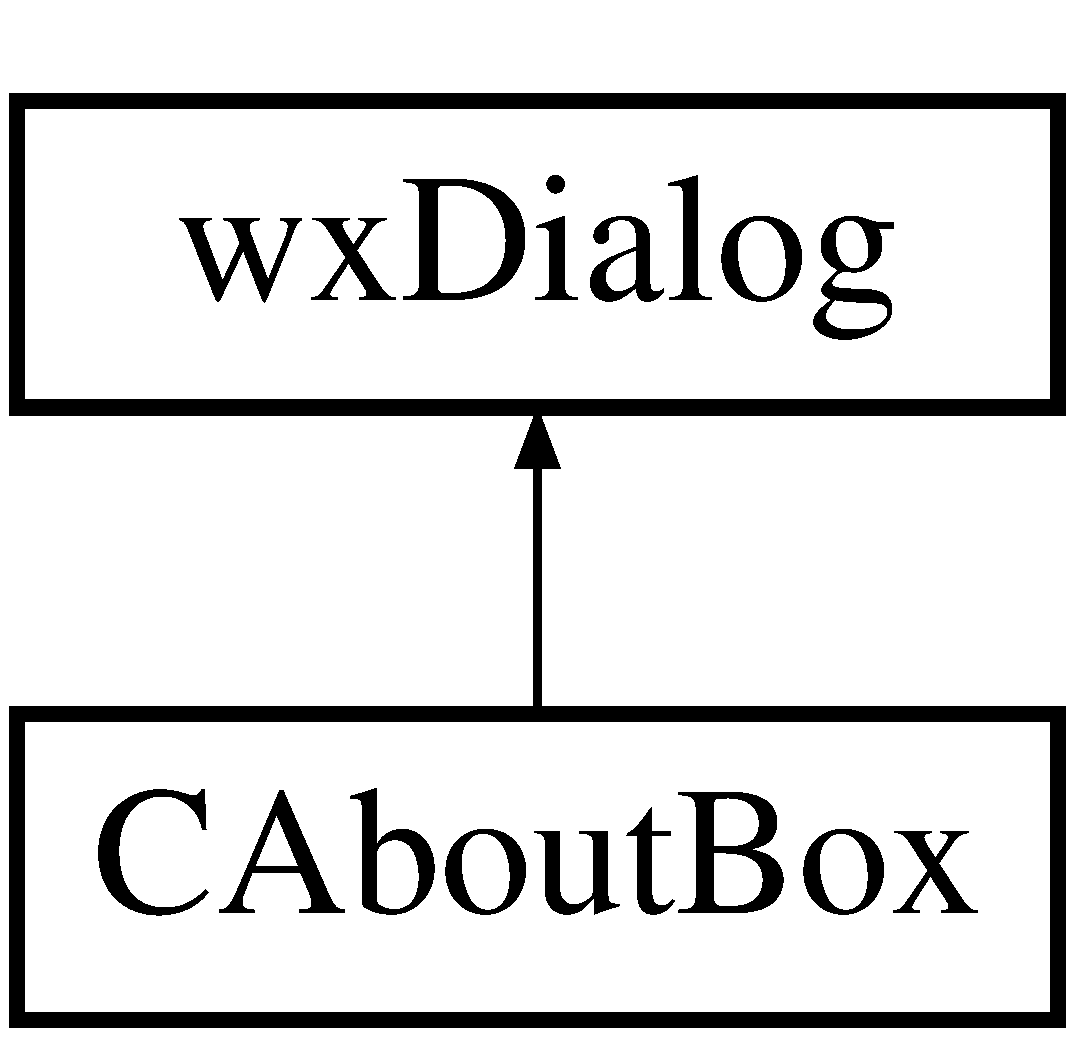
\includegraphics[height=2.000000cm]{classCAboutBox}
\end{center}
\end{figure}
\subsection*{Public Member Functions}
\begin{DoxyCompactItemize}
\item 
\mbox{\Hypertarget{classCAboutBox_ac23aeafcffb40eb72b01da54b7db8e37}\label{classCAboutBox_ac23aeafcffb40eb72b01da54b7db8e37}} 
{\bfseries C\+About\+Box} (wx\+Window $\ast$parent, wx\+Window\+ID id=-\/1)
\end{DoxyCompactItemize}
\subsection*{Static Public Attributes}
\begin{DoxyCompactItemize}
\item 
\mbox{\Hypertarget{classCAboutBox_a8a8c71cf80bae706d4dcab85ea36330f}\label{classCAboutBox_a8a8c71cf80bae706d4dcab85ea36330f}} 
static const long {\bfseries I\+D\+\_\+\+S\+T\+A\+T\+I\+C\+T\+E\+X\+T1} = wx\+New\+Id()
\item 
\mbox{\Hypertarget{classCAboutBox_ad9232b25d16dc3fd4118b66356de9835}\label{classCAboutBox_ad9232b25d16dc3fd4118b66356de9835}} 
static const long {\bfseries I\+D\+\_\+\+S\+T\+A\+T\+I\+C\+T\+E\+X\+T2} = wx\+New\+Id()
\item 
\mbox{\Hypertarget{classCAboutBox_a0a488920494fd9877808ab6161460f50}\label{classCAboutBox_a0a488920494fd9877808ab6161460f50}} 
static const long {\bfseries I\+D\+\_\+\+S\+T\+A\+T\+I\+C\+B\+I\+T\+M\+A\+P1} = wx\+New\+Id()
\item 
\mbox{\Hypertarget{classCAboutBox_a37f53de8b8107dd06c492ede246d1666}\label{classCAboutBox_a37f53de8b8107dd06c492ede246d1666}} 
static const long {\bfseries I\+D\+\_\+\+S\+T\+A\+T\+I\+C\+L\+I\+N\+E1} = wx\+New\+Id()
\item 
\mbox{\Hypertarget{classCAboutBox_a0d649c670b29575cdbfc1f1a1a6ad177}\label{classCAboutBox_a0d649c670b29575cdbfc1f1a1a6ad177}} 
static const long {\bfseries I\+D\+\_\+\+T\+E\+X\+T\+C\+T\+R\+L1} = wx\+New\+Id()
\item 
\mbox{\Hypertarget{classCAboutBox_a6c8d3fabb2794f7bacfcf641aaf23abb}\label{classCAboutBox_a6c8d3fabb2794f7bacfcf641aaf23abb}} 
static const long {\bfseries I\+D\+\_\+\+T\+E\+X\+T\+C\+T\+R\+L2} = wx\+New\+Id()
\item 
\mbox{\Hypertarget{classCAboutBox_ab111166245ba1ed7e7a51820faf25aa3}\label{classCAboutBox_ab111166245ba1ed7e7a51820faf25aa3}} 
static const long {\bfseries I\+D\+\_\+\+T\+E\+X\+T\+C\+T\+R\+L3} = wx\+New\+Id()
\item 
\mbox{\Hypertarget{classCAboutBox_a1b9b6bcf1535e4ba4a6f122d59c74f20}\label{classCAboutBox_a1b9b6bcf1535e4ba4a6f122d59c74f20}} 
static const long {\bfseries I\+D\+\_\+\+N\+O\+T\+E\+B\+O\+O\+K1} = wx\+New\+Id()
\item 
\mbox{\Hypertarget{classCAboutBox_a709e9b214b7b73ecd7f194d1212ba872}\label{classCAboutBox_a709e9b214b7b73ecd7f194d1212ba872}} 
static const long {\bfseries I\+D\+\_\+\+B\+U\+T\+T\+O\+N1} = wx\+New\+Id()
\end{DoxyCompactItemize}
\subsection*{Protected Member Functions}
\begin{DoxyCompactItemize}
\item 
\mbox{\Hypertarget{classCAboutBox_a7b8a029f1bc14a171489139ecf3b9efd}\label{classCAboutBox_a7b8a029f1bc14a171489139ecf3b9efd}} 
void {\bfseries On\+Init} (wx\+Init\+Dialog\+Event \&event)
\item 
\mbox{\Hypertarget{classCAboutBox_a4ceb56a1d2dcdf7ebdbc2db415abcf00}\label{classCAboutBox_a4ceb56a1d2dcdf7ebdbc2db415abcf00}} 
void {\bfseries On\+Button1\+Click} (wx\+Command\+Event \&event)
\item 
\mbox{\Hypertarget{classCAboutBox_a8ba8776862019cee447e0cce4cfa58df}\label{classCAboutBox_a8ba8776862019cee447e0cce4cfa58df}} 
void {\bfseries On\+Char} (wx\+Key\+Event \&event)
\end{DoxyCompactItemize}
\subsection*{Protected Attributes}
\begin{DoxyCompactItemize}
\item 
\mbox{\Hypertarget{classCAboutBox_a0250ce66d89cd0c47107d23d7823b550}\label{classCAboutBox_a0250ce66d89cd0c47107d23d7823b550}} 
wx\+Static\+Text $\ast$ {\bfseries lb\+Prog\+Name}
\item 
\mbox{\Hypertarget{classCAboutBox_a7eb4127fb53f0df92c73ced7c9d8704b}\label{classCAboutBox_a7eb4127fb53f0df92c73ced7c9d8704b}} 
wx\+Flex\+Grid\+Sizer $\ast$ {\bfseries Flex\+Grid\+Sizer1}
\item 
\mbox{\Hypertarget{classCAboutBox_af39fc1e955543ca8e4dc60d900e29339}\label{classCAboutBox_af39fc1e955543ca8e4dc60d900e29339}} 
wx\+Text\+Ctrl $\ast$ {\bfseries lb\+License}
\item 
\mbox{\Hypertarget{classCAboutBox_a6ee2c45e8140523726ae0adac39e5e8d}\label{classCAboutBox_a6ee2c45e8140523726ae0adac39e5e8d}} 
wx\+Button $\ast$ {\bfseries Button1}
\item 
\mbox{\Hypertarget{classCAboutBox_a03cbdcae864388315c72bc1b301cc079}\label{classCAboutBox_a03cbdcae864388315c72bc1b301cc079}} 
wx\+Flex\+Grid\+Sizer $\ast$ {\bfseries Flex\+Grid\+Sizer4}
\item 
\mbox{\Hypertarget{classCAboutBox_a3839eefb2b7f455608fd9e84893fd404}\label{classCAboutBox_a3839eefb2b7f455608fd9e84893fd404}} 
wx\+Static\+Line $\ast$ {\bfseries Static\+Line1}
\item 
\mbox{\Hypertarget{classCAboutBox_ac2602c693f6375acace0ffc56f3a62c5}\label{classCAboutBox_ac2602c693f6375acace0ffc56f3a62c5}} 
wx\+Static\+Text $\ast$ {\bfseries lb\+Build}
\item 
\mbox{\Hypertarget{classCAboutBox_a1b4ced1fdb78e6579f120a14aa1db7ec}\label{classCAboutBox_a1b4ced1fdb78e6579f120a14aa1db7ec}} 
wx\+Text\+Ctrl $\ast$ {\bfseries Text\+Ctrl1}
\item 
\mbox{\Hypertarget{classCAboutBox_a34c7e54c89dca93bdc268582e9b135c4}\label{classCAboutBox_a34c7e54c89dca93bdc268582e9b135c4}} 
wx\+Notebook $\ast$ {\bfseries Notebook1}
\item 
\mbox{\Hypertarget{classCAboutBox_ab8d715f8ada37310f3d43b81b739f979}\label{classCAboutBox_ab8d715f8ada37310f3d43b81b739f979}} 
wx\+Text\+Ctrl $\ast$ {\bfseries lb\+Info}
\item 
\mbox{\Hypertarget{classCAboutBox_ad691d2c2a7dd5252942841d72883ccdd}\label{classCAboutBox_ad691d2c2a7dd5252942841d72883ccdd}} 
wx\+Static\+Bitmap $\ast$ {\bfseries Static\+Bitmap1}
\end{DoxyCompactItemize}


The documentation for this class was generated from the following files\+:\begin{DoxyCompactItemize}
\item 
C\+About\+Box.\+h\item 
C\+About\+Box.\+cpp\end{DoxyCompactItemize}

\hypertarget{classmotion_1_1CActionArc}{}\section{motion\+:\+:C\+Action\+Arc Class Reference}
\label{classmotion_1_1CActionArc}\index{motion\+::\+C\+Action\+Arc@{motion\+::\+C\+Action\+Arc}}
Inheritance diagram for motion\+:\+:C\+Action\+Arc\+:\begin{figure}[H]
\begin{center}
\leavevmode
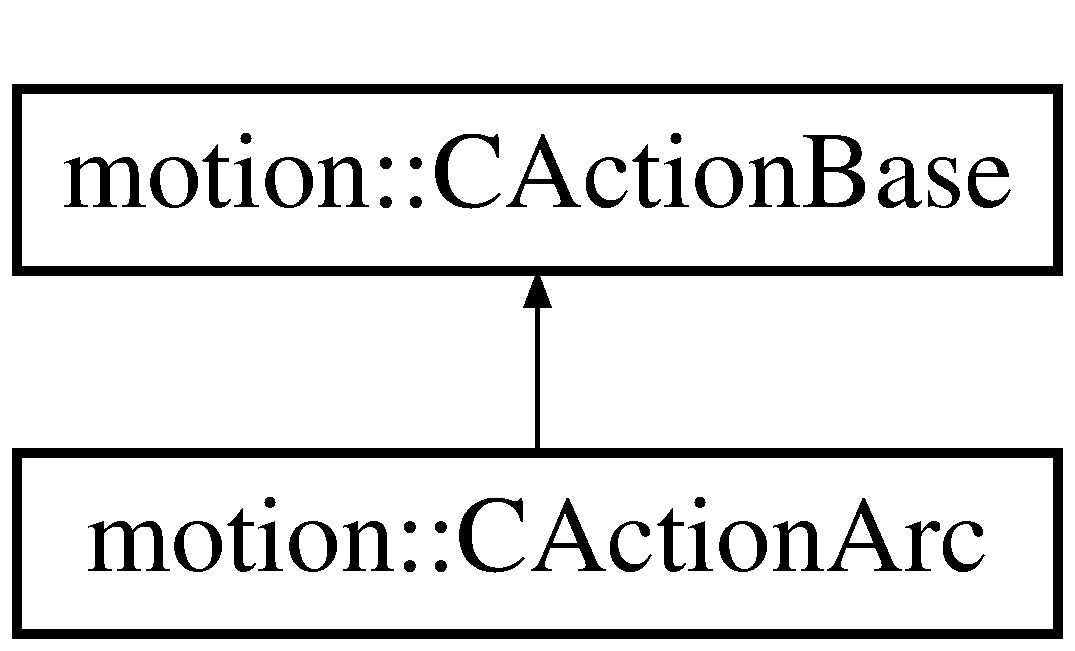
\includegraphics[height=2.000000cm]{classmotion_1_1CActionArc}
\end{center}
\end{figure}
\subsection*{Public Member Functions}
\begin{DoxyCompactItemize}
\item 
\mbox{\Hypertarget{classmotion_1_1CActionArc_a7b8746c8652bb865f2b606608dffbb16}\label{classmotion_1_1CActionArc_a7b8746c8652bb865f2b606608dffbb16}} 
void {\bfseries reset} (void)
\item 
\mbox{\Hypertarget{classmotion_1_1CActionArc_a45356c022471267db143fd1300f6b465}\label{classmotion_1_1CActionArc_a45356c022471267db143fd1300f6b465}} 
void {\bfseries set\+State} (E\+Steering\+State\+Type state)
\item 
\mbox{\Hypertarget{classmotion_1_1CActionArc_ad6f08adc549f8d19892e0a6a257415dc}\label{classmotion_1_1CActionArc_ad6f08adc549f8d19892e0a6a257415dc}} 
void {\bfseries set\+End\+Pose} (\mbox{\hyperlink{structmotion_1_1TMotionPose2D}{T\+Motion\+Pose2D}} pose)
\item 
\mbox{\Hypertarget{classmotion_1_1CActionArc_a6af47c85b3b8226b6ae5bc3e27185e77}\label{classmotion_1_1CActionArc_a6af47c85b3b8226b6ae5bc3e27185e77}} 
void {\bfseries set\+Start\+Up} (bool val)
\item 
\mbox{\Hypertarget{classmotion_1_1CActionArc_ae196348547fee7f670bb91f66b55fa36}\label{classmotion_1_1CActionArc_ae196348547fee7f670bb91f66b55fa36}} 
E\+Steering\+State\+Type {\bfseries get\+State} (void)
\item 
\mbox{\Hypertarget{classmotion_1_1CActionArc_ad5ff8628c709a14cbcffb030894daa93}\label{classmotion_1_1CActionArc_ad5ff8628c709a14cbcffb030894daa93}} 
\mbox{\hyperlink{structmotion_1_1TMotionPose2D}{T\+Motion\+Pose2D}} {\bfseries get\+End\+Pose} (void)
\item 
\mbox{\Hypertarget{classmotion_1_1CActionArc_aa2ee90e89b02256cd0c3f422f220caca}\label{classmotion_1_1CActionArc_aa2ee90e89b02256cd0c3f422f220caca}} 
bool {\bfseries get\+Start\+Up} (void)
\item 
void \mbox{\hyperlink{classmotion_1_1CActionArc_a64a6fc339df29d196786291f02b2802e}{arc}} (double w, double ang\+Deg, double radius=0)
\end{DoxyCompactItemize}
\subsection*{Static Public Member Functions}
\begin{DoxyCompactItemize}
\item 
\mbox{\Hypertarget{classmotion_1_1CActionArc_a058d43888af190cf93dc3130746d9e9e}\label{classmotion_1_1CActionArc_a058d43888af190cf93dc3130746d9e9e}} 
static \mbox{\hyperlink{classmotion_1_1CActionArc}{C\+Action\+Arc}} $\ast$ {\bfseries get\+Instance} (void)
\end{DoxyCompactItemize}


\subsection{Member Function Documentation}
\mbox{\Hypertarget{classmotion_1_1CActionArc_a64a6fc339df29d196786291f02b2802e}\label{classmotion_1_1CActionArc_a64a6fc339df29d196786291f02b2802e}} 
\index{motion\+::\+C\+Action\+Arc@{motion\+::\+C\+Action\+Arc}!arc@{arc}}
\index{arc@{arc}!motion\+::\+C\+Action\+Arc@{motion\+::\+C\+Action\+Arc}}
\subsubsection{\texorpdfstring{arc()}{arc()}}
{\footnotesize\ttfamily void C\+Action\+Arc\+::arc (\begin{DoxyParamCaption}\item[{double}]{w,  }\item[{double}]{ang\+Deg,  }\item[{double}]{radius = {\ttfamily 0} }\end{DoxyParamCaption})}

Make the vehicle make arc. 
\begin{DoxyParams}{Parameters}
{\em w} & Linear velocity(rad/s). w is positive. \\
\hline
{\em angle\+Degree} & The desired angle in degree we want the robot rotate. angle\+Degree $>$ 0 rotate counterclockwise. \\
\hline
{\em radius} & Arc radius. \\
\hline
\end{DoxyParams}
how to avoid multiple tasks? ~\newline
~\newline
~\newline
~\newline
 Start the timer

If start up is enabled, update if the vehicle get started everytime. ~\newline
~\newline
 throw exceptions assert(!\char`\"{}\+Time out when making Arc move.\char`\"{}); ~\newline
 throw exceptions assert(!\char`\"{}\+Direction reached but can\textquotesingle{}t reach the appropriate location.\char`\"{}); 

The documentation for this class was generated from the following files\+:\begin{DoxyCompactItemize}
\item 
motion/action/C\+Action\+Arc.\+h\item 
motion/action/C\+Action\+Arc.\+cpp\end{DoxyCompactItemize}

\hypertarget{classmotion_1_1CActionBackward}{}\section{motion\+:\+:C\+Action\+Backward Class Reference}
\label{classmotion_1_1CActionBackward}\index{motion\+::\+C\+Action\+Backward@{motion\+::\+C\+Action\+Backward}}


{\ttfamily \#include $<$C\+Action\+Backward.\+h$>$}

Inheritance diagram for motion\+:\+:C\+Action\+Backward\+:\begin{figure}[H]
\begin{center}
\leavevmode
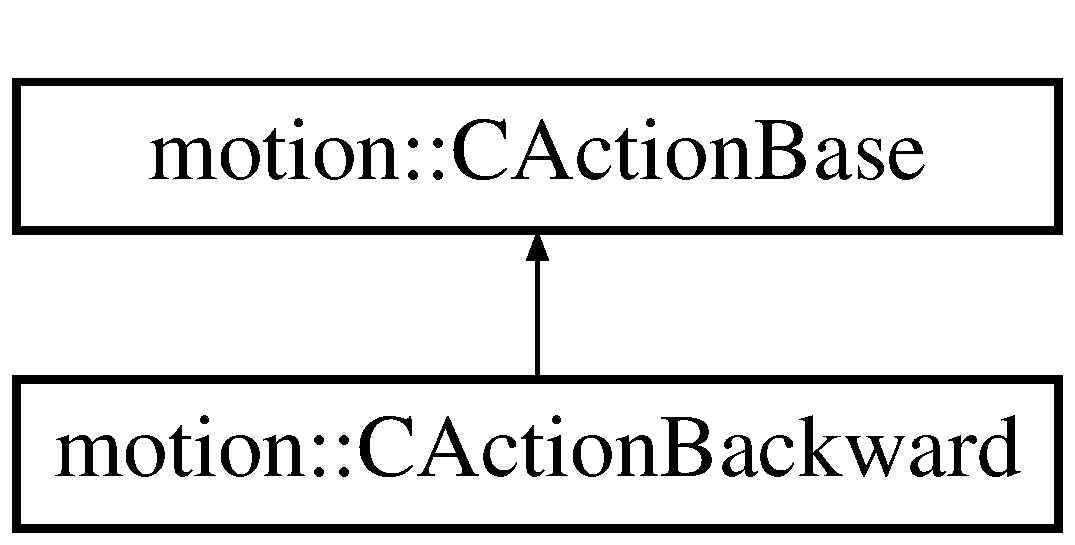
\includegraphics[height=2.000000cm]{classmotion_1_1CActionBackward}
\end{center}
\end{figure}
\subsection*{Public Member Functions}
\begin{DoxyCompactItemize}
\item 
void \mbox{\hyperlink{classmotion_1_1CActionBackward_a609f364c24b4ceebda81c0b591692d2a}{reset}} (void)
\item 
void \mbox{\hyperlink{classmotion_1_1CActionBackward_ab05c93abef4815a4a9f38afeddbb8c2a}{backward}} (double v, double distance)
\end{DoxyCompactItemize}
\subsection*{Static Public Member Functions}
\begin{DoxyCompactItemize}
\item 
\mbox{\Hypertarget{classmotion_1_1CActionBackward_aa1b0a2ac1a8f390bc88b36607137b5f1}\label{classmotion_1_1CActionBackward_aa1b0a2ac1a8f390bc88b36607137b5f1}} 
static \mbox{\hyperlink{classmotion_1_1CActionBackward}{C\+Action\+Backward}} $\ast$ {\bfseries get\+Instance} (void)
\end{DoxyCompactItemize}


\subsection{Detailed Description}
Backward ~\newline
 example\+: ~\newline
 \#include \mbox{\hyperlink{CActionBackward_8h}{C\+Action\+Backward.\+h}} ~\newline
 bkw-\/$>$backward(1, 90); ~\newline
if(bkw-\/$>$get\+Action\+State()==B\+A\+C\+K\+W\+A\+R\+D\+\_\+\+F\+I\+N\+I\+S\+H\+ED) ~\newline
\{ ~\newline
 printf(\char`\"{}\+Backing task finished. Please command the next order.\textbackslash{}n\char`\"{}); ~\newline
\} 

\subsection{Member Function Documentation}
\mbox{\Hypertarget{classmotion_1_1CActionBackward_ab05c93abef4815a4a9f38afeddbb8c2a}\label{classmotion_1_1CActionBackward_ab05c93abef4815a4a9f38afeddbb8c2a}} 
\index{motion\+::\+C\+Action\+Backward@{motion\+::\+C\+Action\+Backward}!backward@{backward}}
\index{backward@{backward}!motion\+::\+C\+Action\+Backward@{motion\+::\+C\+Action\+Backward}}
\subsubsection{\texorpdfstring{backward()}{backward()}}
{\footnotesize\ttfamily void C\+Action\+Backward\+::backward (\begin{DoxyParamCaption}\item[{double}]{v,  }\item[{double}]{distance }\end{DoxyParamCaption})}

Move the robot backward straightly. 
\begin{DoxyParams}{Parameters}
{\em v} & The backward linear velocity. \\
\hline
{\em distance} & The desired distance we want the robot backward. \\
\hline
\end{DoxyParams}
Store current information and calculate information needed

start the timer

Timeout check.

throw exceptions assert(!\char`\"{}\+Time out when backwarding.\char`\"{}); ~\newline
 Finish condition check. \mbox{\Hypertarget{classmotion_1_1CActionBackward_a609f364c24b4ceebda81c0b591692d2a}\label{classmotion_1_1CActionBackward_a609f364c24b4ceebda81c0b591692d2a}} 
\index{motion\+::\+C\+Action\+Backward@{motion\+::\+C\+Action\+Backward}!reset@{reset}}
\index{reset@{reset}!motion\+::\+C\+Action\+Backward@{motion\+::\+C\+Action\+Backward}}
\subsubsection{\texorpdfstring{reset()}{reset()}}
{\footnotesize\ttfamily void C\+Action\+Backward\+::reset (\begin{DoxyParamCaption}\item[{void}]{ }\end{DoxyParamCaption})}

$<$ Reset base private variables. 

The documentation for this class was generated from the following files\+:\begin{DoxyCompactItemize}
\item 
motion/action/\mbox{\hyperlink{CActionBackward_8h}{C\+Action\+Backward.\+h}}\item 
motion/action/\mbox{\hyperlink{CActionBackward_8cpp}{C\+Action\+Backward.\+cpp}}\end{DoxyCompactItemize}

\hypertarget{classmotion_1_1CActionBase}{}\section{motion\+:\+:C\+Action\+Base Class Reference}
\label{classmotion_1_1CActionBase}\index{motion\+::\+C\+Action\+Base@{motion\+::\+C\+Action\+Base}}


{\ttfamily \#include $<$C\+Action\+Base.\+h$>$}

Inheritance diagram for motion\+:\+:C\+Action\+Base\+:\begin{figure}[H]
\begin{center}
\leavevmode
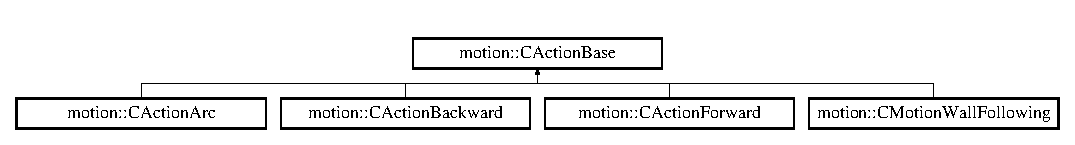
\includegraphics[height=0.855615cm]{classmotion_1_1CActionBase}
\end{center}
\end{figure}
\subsection*{Public Member Functions}
\begin{DoxyCompactItemize}
\item 
\mbox{\Hypertarget{classmotion_1_1CActionBase_ab64789ff634b40a7c88771186deb02b3}\label{classmotion_1_1CActionBase_ab64789ff634b40a7c88771186deb02b3}} 
void {\bfseries reset\+Base} (void)
\item 
\mbox{\Hypertarget{classmotion_1_1CActionBase_a56290a85c15b62718137f4a79a0e5d24}\label{classmotion_1_1CActionBase_a56290a85c15b62718137f4a79a0e5d24}} 
double {\bfseries get\+Ahead\+Dist} (void) const
\item 
\mbox{\Hypertarget{classmotion_1_1CActionBase_adee7bb394fc82f936af57e997ccc1f7f}\label{classmotion_1_1CActionBase_adee7bb394fc82f936af57e997ccc1f7f}} 
double {\bfseries get\+Side\+Dist} (void) const
\item 
\mbox{\Hypertarget{classmotion_1_1CActionBase_ab7cac53d714c3688609f5bfb026c6c4f}\label{classmotion_1_1CActionBase_ab7cac53d714c3688609f5bfb026c6c4f}} 
double {\bfseries get\+Linear\+Velocity} (void) const
\item 
\mbox{\Hypertarget{classmotion_1_1CActionBase_aba9b4953364ac77f49e98ea6f59a3aad}\label{classmotion_1_1CActionBase_aba9b4953364ac77f49e98ea6f59a3aad}} 
void {\bfseries set\+Velocity} (double v, double w)
\item 
\mbox{\Hypertarget{classmotion_1_1CActionBase_ab83e2ccbad3a796da9c8013467f89a5d}\label{classmotion_1_1CActionBase_ab83e2ccbad3a796da9c8013467f89a5d}} 
void {\bfseries set\+Motion} (\mbox{\hyperlink{motionEnums_8h_a907f80786f402332d43f4646dc1450bc}{E\+Motion}} mot)
\item 
\mbox{\Hypertarget{classmotion_1_1CActionBase_a97b30f5e328649e00b8c3889ef6fce4a}\label{classmotion_1_1CActionBase_a97b30f5e328649e00b8c3889ef6fce4a}} 
void {\bfseries set\+Sub\+Motion} (\mbox{\hyperlink{motionEnums_8h_a23be5ef75af9219a8bf688fd9716d72c}{E\+Sub\+Motion}} submot)
\item 
\mbox{\Hypertarget{classmotion_1_1CActionBase_a82ea8bab8f8a6ccfe0f4cf4addc47d33}\label{classmotion_1_1CActionBase_a82ea8bab8f8a6ccfe0f4cf4addc47d33}} 
void {\bfseries set\+Sub\+Motion\+State} (\mbox{\hyperlink{motionEnums_8h_a272f94c6143b9acf7ac44f165be53948}{E\+Sub\+Motion\+State}} submotstate)
\item 
\mbox{\Hypertarget{classmotion_1_1CActionBase_aa5ea8ef039688efb9da75e552bfff955}\label{classmotion_1_1CActionBase_aa5ea8ef039688efb9da75e552bfff955}} 
void {\bfseries set\+Action} (\mbox{\hyperlink{motionEnums_8h_aa7486027d362655230b958efe6985a7f}{E\+Action}} act) const
\item 
\mbox{\Hypertarget{classmotion_1_1CActionBase_a37cf7cf8e21e5df22d1ae5326e92db63}\label{classmotion_1_1CActionBase_a37cf7cf8e21e5df22d1ae5326e92db63}} 
void {\bfseries set\+Action\+State} (\mbox{\hyperlink{motionEnums_8h_ac80e838bea11b75469bfc14b1de921a3}{E\+Action\+State}} actsta)
\item 
\mbox{\Hypertarget{classmotion_1_1CActionBase_a9c30abb08480e7b0cbd8a2d1bd2289a9}\label{classmotion_1_1CActionBase_a9c30abb08480e7b0cbd8a2d1bd2289a9}} 
\mbox{\hyperlink{motionEnums_8h_a907f80786f402332d43f4646dc1450bc}{E\+Motion}} {\bfseries get\+Motion} (void) const
\item 
\mbox{\Hypertarget{classmotion_1_1CActionBase_ade6e14ed3cdb446bc146c4188d845547}\label{classmotion_1_1CActionBase_ade6e14ed3cdb446bc146c4188d845547}} 
\mbox{\hyperlink{motionEnums_8h_a23be5ef75af9219a8bf688fd9716d72c}{E\+Sub\+Motion}} {\bfseries get\+Sub\+Motion} (void) const
\item 
\mbox{\Hypertarget{classmotion_1_1CActionBase_a51e0207c21bc6da29b0435dead1dd6cc}\label{classmotion_1_1CActionBase_a51e0207c21bc6da29b0435dead1dd6cc}} 
\mbox{\hyperlink{motionEnums_8h_a272f94c6143b9acf7ac44f165be53948}{E\+Sub\+Motion\+State}} {\bfseries get\+Sub\+Motion\+State} (void) const
\item 
\mbox{\Hypertarget{classmotion_1_1CActionBase_a14d5ba8c773b1abb71974777daa5e0da}\label{classmotion_1_1CActionBase_a14d5ba8c773b1abb71974777daa5e0da}} 
\mbox{\hyperlink{motionEnums_8h_aa7486027d362655230b958efe6985a7f}{E\+Action}} {\bfseries get\+Action} (void) const
\item 
\mbox{\Hypertarget{classmotion_1_1CActionBase_af0210e352a49c47ad7a7a2d2d8145a63}\label{classmotion_1_1CActionBase_af0210e352a49c47ad7a7a2d2d8145a63}} 
\mbox{\hyperlink{motionEnums_8h_ac80e838bea11b75469bfc14b1de921a3}{E\+Action\+State}} {\bfseries get\+Action\+State} (void) const
\item 
\mbox{\Hypertarget{classmotion_1_1CActionBase_a6c91610ed7b320cfc5ed13cfea9494b5}\label{classmotion_1_1CActionBase_a6c91610ed7b320cfc5ed13cfea9494b5}} 
double {\bfseries get\+Angular\+Velocity} (void)
\item 
\mbox{\Hypertarget{classmotion_1_1CActionBase_a7fcc833fc87392ea9f8990217c699990}\label{classmotion_1_1CActionBase_a7fcc833fc87392ea9f8990217c699990}} 
bool {\bfseries get\+Pose\+Stored} (void) const
\item 
\mbox{\Hypertarget{classmotion_1_1CActionBase_a1e4ce35712fb80d112e93f4c0025a17a}\label{classmotion_1_1CActionBase_a1e4ce35712fb80d112e93f4c0025a17a}} 
void {\bfseries set\+Pose\+Stored} (bool flag)
\item 
\mbox{\Hypertarget{classmotion_1_1CActionBase_ac576f7b9fffaa9b682b78e3737d73e36}\label{classmotion_1_1CActionBase_ac576f7b9fffaa9b682b78e3737d73e36}} 
\mbox{\hyperlink{structmotion_1_1TMotionPose2D}{T\+Motion\+Pose2D}} {\bfseries get\+Start\+Pose} (void) const
\item 
\mbox{\Hypertarget{classmotion_1_1CActionBase_a0c58bcd69d90d6c89b1a6eef002c6565}\label{classmotion_1_1CActionBase_a0c58bcd69d90d6c89b1a6eef002c6565}} 
\mbox{\hyperlink{structmotion_1_1TMotionPose2D}{T\+Motion\+Pose2D}} {\bfseries get\+Cur\+Pose} (void) const
\item 
\mbox{\Hypertarget{classmotion_1_1CActionBase_a5fab5515a22960387aec3e3edd3dc6d8}\label{classmotion_1_1CActionBase_a5fab5515a22960387aec3e3edd3dc6d8}} 
double {\bfseries get\+Time\+Needed} (void)
\item 
void \mbox{\hyperlink{classmotion_1_1CActionBase_aa00772ca5a67bce272f0872bcc34baa6}{set\+Motion\+Params}} (\mbox{\hyperlink{structmotion_1_1TMotionParams}{T\+Motion\+Params}} param)
\item 
\mbox{\Hypertarget{classmotion_1_1CActionBase_a579a415b15c4fb52fd85e6c87784b3f9}\label{classmotion_1_1CActionBase_a579a415b15c4fb52fd85e6c87784b3f9}} 
\mbox{\hyperlink{structmotion_1_1TMotionParams}{T\+Motion\+Params}} {\bfseries get\+Motion\+Params} (void)
\item 
\mbox{\Hypertarget{classmotion_1_1CActionBase_ad1f558f309fab3a0f480e627ad11fdcc}\label{classmotion_1_1CActionBase_ad1f558f309fab3a0f480e627ad11fdcc}} 
void {\bfseries set\+Pre\+Phi} (double pp)
\item 
\mbox{\Hypertarget{classmotion_1_1CActionBase_ad6efc8e152e80cc56e6f48b2c3fce901}\label{classmotion_1_1CActionBase_ad6efc8e152e80cc56e6f48b2c3fce901}} 
double {\bfseries get\+Pre\+Phi} (void) const
\item 
\mbox{\Hypertarget{classmotion_1_1CActionBase_a934dc54034551a3781a5a193bc67268f}\label{classmotion_1_1CActionBase_a934dc54034551a3781a5a193bc67268f}} 
void {\bfseries set\+Jump\+Count} (int jc)
\item 
\mbox{\Hypertarget{classmotion_1_1CActionBase_afe65cb32174b7c3a84623a1da8293594}\label{classmotion_1_1CActionBase_afe65cb32174b7c3a84623a1da8293594}} 
int {\bfseries get\+Jump\+Count} (void) const
\item 
\mbox{\Hypertarget{classmotion_1_1CActionBase_af2c6d7fc26e2bf35184eb8062b121522}\label{classmotion_1_1CActionBase_af2c6d7fc26e2bf35184eb8062b121522}} 
void {\bfseries set\+Jump\+Dir} (\mbox{\hyperlink{motionEnums_8h_a03a5344cd29a761a4b7dcaf1df3c3c85}{E\+Rotate\+Side}} rs)
\item 
\mbox{\Hypertarget{classmotion_1_1CActionBase_a44b1d1fa8bedfa59916d9c4c31b22117}\label{classmotion_1_1CActionBase_a44b1d1fa8bedfa59916d9c4c31b22117}} 
\mbox{\hyperlink{motionEnums_8h_a03a5344cd29a761a4b7dcaf1df3c3c85}{E\+Rotate\+Side}} {\bfseries get\+Jump\+Dir} (void) const
\item 
\mbox{\Hypertarget{classmotion_1_1CActionBase_a1a90c80a9029798aac8b2fd388d8f784}\label{classmotion_1_1CActionBase_a1a90c80a9029798aac8b2fd388d8f784}} 
void {\bfseries set\+Positive} (\mbox{\hyperlink{motionEnums_8h_a03a5344cd29a761a4b7dcaf1df3c3c85}{E\+Rotate\+Side}} rs)
\item 
\mbox{\Hypertarget{classmotion_1_1CActionBase_a5c84487dba7d2996e9d35376b7a45c79}\label{classmotion_1_1CActionBase_a5c84487dba7d2996e9d35376b7a45c79}} 
\mbox{\hyperlink{motionEnums_8h_a03a5344cd29a761a4b7dcaf1df3c3c85}{E\+Rotate\+Side}} {\bfseries get\+Positive} (void) const
\item 
\mbox{\Hypertarget{classmotion_1_1CActionBase_a595c2b53e4daf353c7855302f626c694}\label{classmotion_1_1CActionBase_a595c2b53e4daf353c7855302f626c694}} 
void {\bfseries set\+Jump\+Count} (bool ps)
\item 
\mbox{\Hypertarget{classmotion_1_1CActionBase_adb60bce8bcb7410ba5596906d64490b0}\label{classmotion_1_1CActionBase_adb60bce8bcb7410ba5596906d64490b0}} 
bool {\bfseries get\+Positive\+Set} (void) const
\item 
void \mbox{\hyperlink{classmotion_1_1CActionBase_a48d2c07fa908bf6ed57e3219a017b25e}{capture\+Jump}} (void)
\item 
void \mbox{\hyperlink{classmotion_1_1CActionBase_a5fd00b2fca445758e6cbf4d5a92a5082}{update\+Cur\+Pose}} (mrpt\+::kinematics\+::\+C\+Vehicle\+Simul\+\_\+\+Diff\+Driven $\ast$robot)
\item 
void \mbox{\hyperlink{classmotion_1_1CActionBase_ac7706bd708dc987b1da17bfa6d33a70c}{update\+Dist}} (mrpt\+::obs\+::\+C\+Observation2\+D\+Range\+Scan $\ast$scan, size\+\_\+t win\+Length)
\item 
\mbox{\hyperlink{structmotion_1_1TMotionPose2D}{T\+Motion\+Pose2D}} \mbox{\hyperlink{classmotion_1_1CActionBase_aef651b6dae673bb2eba9245aa509c40d}{frame\+Rot}} (double x, double y, double phi\+Rad)
\item 
void \mbox{\hyperlink{classmotion_1_1CActionBase_af660bbf31c33b1932a1a5b9219334211}{store\+Start\+Pose}} (void)
\item 
void \mbox{\hyperlink{classmotion_1_1CActionBase_a90058a23162d40496c60ed44578c2f69}{calc\+Time\+Needed}} (double velocity, double displacement)
\end{DoxyCompactItemize}


\subsection{Detailed Description}
Base class ~\newline


\subsection{Member Function Documentation}
\mbox{\Hypertarget{classmotion_1_1CActionBase_a90058a23162d40496c60ed44578c2f69}\label{classmotion_1_1CActionBase_a90058a23162d40496c60ed44578c2f69}} 
\index{motion\+::\+C\+Action\+Base@{motion\+::\+C\+Action\+Base}!calc\+Time\+Needed@{calc\+Time\+Needed}}
\index{calc\+Time\+Needed@{calc\+Time\+Needed}!motion\+::\+C\+Action\+Base@{motion\+::\+C\+Action\+Base}}
\subsubsection{\texorpdfstring{calc\+Time\+Needed()}{calcTimeNeeded()}}
{\footnotesize\ttfamily void C\+Action\+Base\+::calc\+Time\+Needed (\begin{DoxyParamCaption}\item[{double}]{velocity,  }\item[{double}]{displacement }\end{DoxyParamCaption})}

Calculate time needed . Used to calculate end pose and verify end pose conditions. \mbox{\Hypertarget{classmotion_1_1CActionBase_a48d2c07fa908bf6ed57e3219a017b25e}\label{classmotion_1_1CActionBase_a48d2c07fa908bf6ed57e3219a017b25e}} 
\index{motion\+::\+C\+Action\+Base@{motion\+::\+C\+Action\+Base}!capture\+Jump@{capture\+Jump}}
\index{capture\+Jump@{capture\+Jump}!motion\+::\+C\+Action\+Base@{motion\+::\+C\+Action\+Base}}
\subsubsection{\texorpdfstring{capture\+Jump()}{captureJump()}}
{\footnotesize\ttfamily void C\+Action\+Base\+::capture\+Jump (\begin{DoxyParamCaption}\item[{void}]{ }\end{DoxyParamCaption})}

Call this method in update\+Cur\+Pose to capture jumps -\/180-\/$>$180 and -\/180-\/$>$180 \begin{DoxySeeAlso}{See also}
\mbox{\hyperlink{classmotion_1_1CActionBase_a5fd00b2fca445758e6cbf4d5a92a5082}{update\+Cur\+Pose}} 
\end{DoxySeeAlso}
printf(\char`\"{}$\ast$$\ast$jump is\+: \%.\+3f\textbackslash{}n\char`\"{}, jump\+Ang\+Deg);

printf(\char`\"{}no jumps.\textbackslash{}n\char`\"{}); \mbox{\Hypertarget{classmotion_1_1CActionBase_aef651b6dae673bb2eba9245aa509c40d}\label{classmotion_1_1CActionBase_aef651b6dae673bb2eba9245aa509c40d}} 
\index{motion\+::\+C\+Action\+Base@{motion\+::\+C\+Action\+Base}!frame\+Rot@{frame\+Rot}}
\index{frame\+Rot@{frame\+Rot}!motion\+::\+C\+Action\+Base@{motion\+::\+C\+Action\+Base}}
\subsubsection{\texorpdfstring{frame\+Rot()}{frameRot()}}
{\footnotesize\ttfamily \mbox{\hyperlink{structmotion_1_1TMotionPose2D}{T\+Motion\+Pose2D}} C\+Action\+Base\+::frame\+Rot (\begin{DoxyParamCaption}\item[{double}]{x,  }\item[{double}]{y,  }\item[{double}]{phi\+Rad }\end{DoxyParamCaption})}

Frame rotation. This method transfers p0=(x0, y0) in frame 0 to p1=(x1, y1) in frame 1, with phi\+Rad angle difference between frame 0 and frame 1. 
\begin{DoxyParams}{Parameters}
{\em x} & p0\textquotesingle{}s X axis coordinates. \\
\hline
{\em y} & p0\textquotesingle{}s Y axis coordinates. \\
\hline
{\em phi\+Rad} & angle difference between frame 0 and frame 1 in rad. Positive means rotate counterc clockwise. \\
\hline
\end{DoxyParams}
\begin{DoxyReturn}{Returns}
p1 
\end{DoxyReturn}
Rotation matrix\+: $\vert$ cos(0) sin(0) 0 $\vert$ ~\newline
 R = $\vert$ -\/sin(0) cos(0) 0 $\vert$ ~\newline
 $\vert$ 0 0 1 $\vert$ ~\newline
 \mbox{\Hypertarget{classmotion_1_1CActionBase_aa00772ca5a67bce272f0872bcc34baa6}\label{classmotion_1_1CActionBase_aa00772ca5a67bce272f0872bcc34baa6}} 
\index{motion\+::\+C\+Action\+Base@{motion\+::\+C\+Action\+Base}!set\+Motion\+Params@{set\+Motion\+Params}}
\index{set\+Motion\+Params@{set\+Motion\+Params}!motion\+::\+C\+Action\+Base@{motion\+::\+C\+Action\+Base}}
\subsubsection{\texorpdfstring{set\+Motion\+Params()}{setMotionParams()}}
{\footnotesize\ttfamily void C\+Action\+Base\+::set\+Motion\+Params (\begin{DoxyParamCaption}\item[{\mbox{\hyperlink{structmotion_1_1TMotionParams}{T\+Motion\+Params}}}]{param }\end{DoxyParamCaption})}

N\+O\+T\+H\+I\+NG \mbox{\Hypertarget{classmotion_1_1CActionBase_af660bbf31c33b1932a1a5b9219334211}\label{classmotion_1_1CActionBase_af660bbf31c33b1932a1a5b9219334211}} 
\index{motion\+::\+C\+Action\+Base@{motion\+::\+C\+Action\+Base}!store\+Start\+Pose@{store\+Start\+Pose}}
\index{store\+Start\+Pose@{store\+Start\+Pose}!motion\+::\+C\+Action\+Base@{motion\+::\+C\+Action\+Base}}
\subsubsection{\texorpdfstring{store\+Start\+Pose()}{storeStartPose()}}
{\footnotesize\ttfamily void C\+Action\+Base\+::store\+Start\+Pose (\begin{DoxyParamCaption}\item[{void}]{ }\end{DoxyParamCaption})}

Store start pose. Used to calculate end pose and verify end pose conditions. Set the pose-\/stored flag. \mbox{\Hypertarget{classmotion_1_1CActionBase_a5fd00b2fca445758e6cbf4d5a92a5082}\label{classmotion_1_1CActionBase_a5fd00b2fca445758e6cbf4d5a92a5082}} 
\index{motion\+::\+C\+Action\+Base@{motion\+::\+C\+Action\+Base}!update\+Cur\+Pose@{update\+Cur\+Pose}}
\index{update\+Cur\+Pose@{update\+Cur\+Pose}!motion\+::\+C\+Action\+Base@{motion\+::\+C\+Action\+Base}}
\subsubsection{\texorpdfstring{update\+Cur\+Pose()}{updateCurPose()}}
{\footnotesize\ttfamily void C\+Action\+Base\+::update\+Cur\+Pose (\begin{DoxyParamCaption}\item[{mrpt\+::kinematics\+::\+C\+Vehicle\+Simul\+\_\+\+Diff\+Driven $\ast$}]{robot }\end{DoxyParamCaption})}

Remove later. \mbox{\Hypertarget{classmotion_1_1CActionBase_ac7706bd708dc987b1da17bfa6d33a70c}\label{classmotion_1_1CActionBase_ac7706bd708dc987b1da17bfa6d33a70c}} 
\index{motion\+::\+C\+Action\+Base@{motion\+::\+C\+Action\+Base}!update\+Dist@{update\+Dist}}
\index{update\+Dist@{update\+Dist}!motion\+::\+C\+Action\+Base@{motion\+::\+C\+Action\+Base}}
\subsubsection{\texorpdfstring{update\+Dist()}{updateDist()}}
{\footnotesize\ttfamily void C\+Action\+Base\+::update\+Dist (\begin{DoxyParamCaption}\item[{mrpt\+::obs\+::\+C\+Observation2\+D\+Range\+Scan $\ast$}]{scan,  }\item[{size\+\_\+t}]{win\+Length }\end{DoxyParamCaption})}

Calculate the distance between robot and wall in the heading direction. And calculate the distance between robot and wall on right side. 
\begin{DoxyParams}{Parameters}
{\em scan} & Pointer that points to the laser object. \\
\hline
{\em win\+Length} & How many data points needed to calculate the distance. \\
\hline
\end{DoxyParams}
\begin{DoxyReturn}{Returns}
Distance. 
\end{DoxyReturn}
Calculate side distance.

printf(\char`\"{}side\+Dist\+: \%.\+3f\textbackslash{}n\char`\"{}, sm\+\_\+motion.\+side\+Dist);

Calculate ahead distance. 

The documentation for this class was generated from the following files\+:\begin{DoxyCompactItemize}
\item 
motion/action/\mbox{\hyperlink{CActionBase_8h}{C\+Action\+Base.\+h}}\item 
motion/action/\mbox{\hyperlink{CActionBase_8cpp}{C\+Action\+Base.\+cpp}}\end{DoxyCompactItemize}

\hypertarget{classmotion_1_1CActionForward}{}\section{motion\+:\+:C\+Action\+Forward Class Reference}
\label{classmotion_1_1CActionForward}\index{motion\+::\+C\+Action\+Forward@{motion\+::\+C\+Action\+Forward}}
Inheritance diagram for motion\+:\+:C\+Action\+Forward\+:\begin{figure}[H]
\begin{center}
\leavevmode
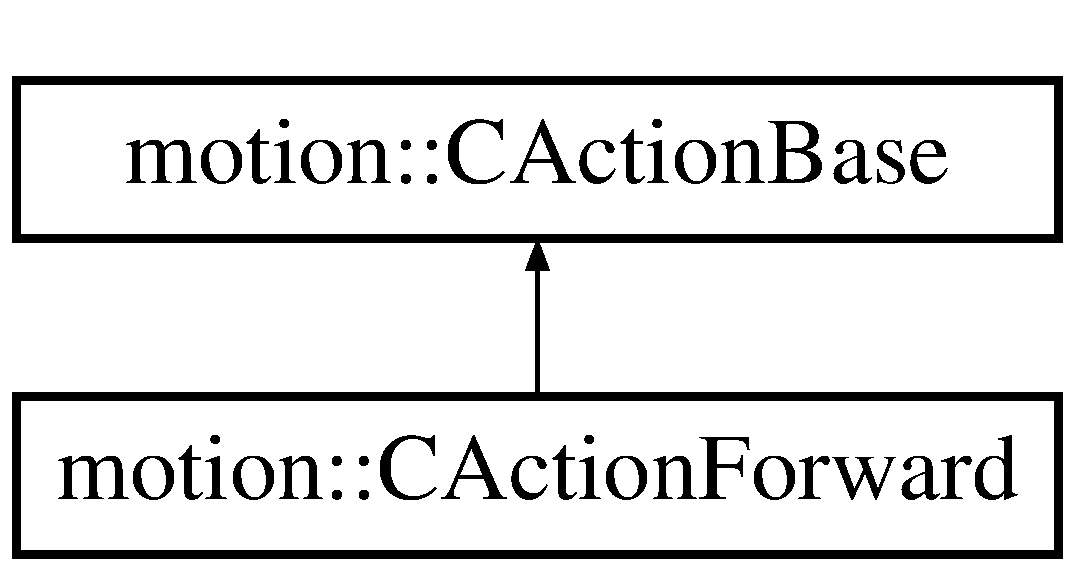
\includegraphics[height=2.000000cm]{classmotion_1_1CActionForward}
\end{center}
\end{figure}
\subsection*{Public Member Functions}
\begin{DoxyCompactItemize}
\item 
void \mbox{\hyperlink{classmotion_1_1CActionForward_af7c72ffee0c2f41c8608259ef3268f23}{reset}} (void)
\item 
\mbox{\Hypertarget{classmotion_1_1CActionForward_af986e75f2773dced403311b3e5e1d7b8}\label{classmotion_1_1CActionForward_af986e75f2773dced403311b3e5e1d7b8}} 
E\+Steering\+State\+Type {\bfseries get\+State} (void)
\item 
\mbox{\Hypertarget{classmotion_1_1CActionForward_a0a17ba177738541886131deca36c6bf1}\label{classmotion_1_1CActionForward_a0a17ba177738541886131deca36c6bf1}} 
void {\bfseries set\+State} (E\+Steering\+State\+Type state)
\item 
void \mbox{\hyperlink{classmotion_1_1CActionForward_abc4d3b39f49514f9d3f64a92393aa6d2}{forward}} (double v, double distance)
\end{DoxyCompactItemize}
\subsection*{Static Public Member Functions}
\begin{DoxyCompactItemize}
\item 
\mbox{\Hypertarget{classmotion_1_1CActionForward_a7820340aa671aaf37c16b945f023b82f}\label{classmotion_1_1CActionForward_a7820340aa671aaf37c16b945f023b82f}} 
static \mbox{\hyperlink{classmotion_1_1CActionForward}{C\+Action\+Forward}} $\ast$ {\bfseries get\+Instance} (void)
\end{DoxyCompactItemize}


\subsection{Member Function Documentation}
\mbox{\Hypertarget{classmotion_1_1CActionForward_abc4d3b39f49514f9d3f64a92393aa6d2}\label{classmotion_1_1CActionForward_abc4d3b39f49514f9d3f64a92393aa6d2}} 
\index{motion\+::\+C\+Action\+Forward@{motion\+::\+C\+Action\+Forward}!forward@{forward}}
\index{forward@{forward}!motion\+::\+C\+Action\+Forward@{motion\+::\+C\+Action\+Forward}}
\subsubsection{\texorpdfstring{forward()}{forward()}}
{\footnotesize\ttfamily void C\+Action\+Forward\+::forward (\begin{DoxyParamCaption}\item[{double}]{v,  }\item[{double}]{distance }\end{DoxyParamCaption})}

Move the robot forward straightly. 
\begin{DoxyParams}{Parameters}
{\em v} & is the forward linear velocity. \\
\hline
{\em distance} & is the desired distance we want the robot forward. \\
\hline
\end{DoxyParams}
start the timer \mbox{\Hypertarget{classmotion_1_1CActionForward_af7c72ffee0c2f41c8608259ef3268f23}\label{classmotion_1_1CActionForward_af7c72ffee0c2f41c8608259ef3268f23}} 
\index{motion\+::\+C\+Action\+Forward@{motion\+::\+C\+Action\+Forward}!reset@{reset}}
\index{reset@{reset}!motion\+::\+C\+Action\+Forward@{motion\+::\+C\+Action\+Forward}}
\subsubsection{\texorpdfstring{reset()}{reset()}}
{\footnotesize\ttfamily void C\+Action\+Forward\+::reset (\begin{DoxyParamCaption}\item[{void}]{ }\end{DoxyParamCaption})}

$<$ Reset base private variables. 

The documentation for this class was generated from the following files\+:\begin{DoxyCompactItemize}
\item 
motion/action/C\+Action\+Forward.\+h\item 
motion/action/C\+Action\+Forward.\+cpp\end{DoxyCompactItemize}

\hypertarget{classmotion_1_1CIdIdle}{}\section{motion\+:\+:C\+Id\+Idle Class Reference}
\label{classmotion_1_1CIdIdle}\index{motion\+::\+C\+Id\+Idle@{motion\+::\+C\+Id\+Idle}}
Inheritance diagram for motion\+:\+:C\+Id\+Idle\+:\begin{figure}[H]
\begin{center}
\leavevmode
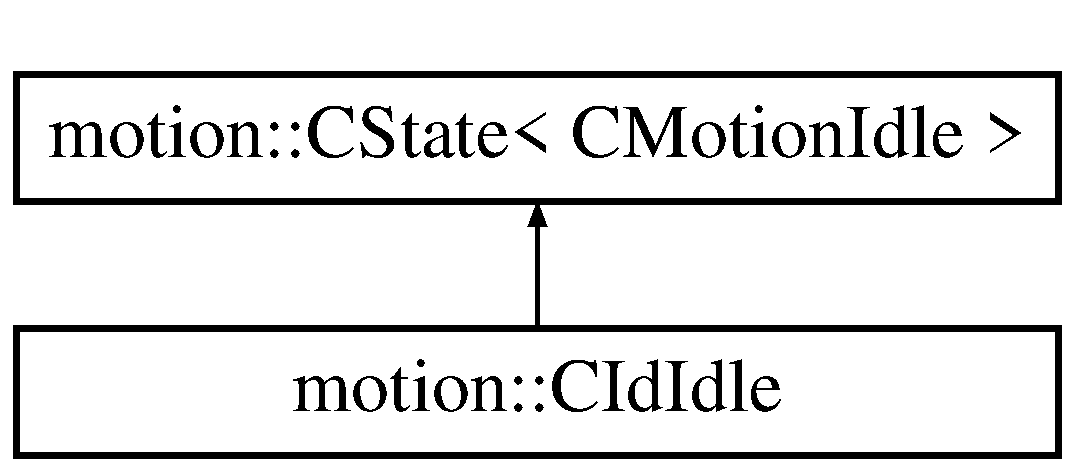
\includegraphics[height=2.000000cm]{classmotion_1_1CIdIdle}
\end{center}
\end{figure}
\subsection*{Public Member Functions}
\begin{DoxyCompactItemize}
\item 
virtual void \mbox{\hyperlink{classmotion_1_1CIdIdle_a14a7339e10f93b2725b6edfb66583ca7}{enter}} (\mbox{\hyperlink{classmotion_1_1CMotionIdle}{C\+Motion\+Idle}} $\ast$id)
\item 
virtual void \mbox{\hyperlink{classmotion_1_1CIdIdle_a157fe57e41c2a53bb5bbd444a74636bd}{execute}} (\mbox{\hyperlink{classmotion_1_1CMotionIdle}{C\+Motion\+Idle}} $\ast$id)
\item 
virtual void \mbox{\hyperlink{classmotion_1_1CIdIdle_aa54a27090c4f10a9a2c5130d9baf14a3}{exit}} (\mbox{\hyperlink{classmotion_1_1CMotionIdle}{C\+Motion\+Idle}} $\ast$id)
\end{DoxyCompactItemize}
\subsection*{Static Public Member Functions}
\begin{DoxyCompactItemize}
\item 
static \mbox{\hyperlink{classmotion_1_1CIdIdle}{C\+Id\+Idle}} $\ast$ \mbox{\hyperlink{classmotion_1_1CIdIdle_ad2a189a219ab9030d99b46a286761b63}{get\+Instance}} (void)
\end{DoxyCompactItemize}


\subsection{Member Function Documentation}
\mbox{\Hypertarget{classmotion_1_1CIdIdle_a14a7339e10f93b2725b6edfb66583ca7}\label{classmotion_1_1CIdIdle_a14a7339e10f93b2725b6edfb66583ca7}} 
\index{motion\+::\+C\+Id\+Idle@{motion\+::\+C\+Id\+Idle}!enter@{enter}}
\index{enter@{enter}!motion\+::\+C\+Id\+Idle@{motion\+::\+C\+Id\+Idle}}
\subsubsection{\texorpdfstring{enter()}{enter()}}
{\footnotesize\ttfamily void C\+Id\+Idle\+::enter (\begin{DoxyParamCaption}\item[{\mbox{\hyperlink{classmotion_1_1CMotionIdle}{C\+Motion\+Idle}} $\ast$}]{ }\end{DoxyParamCaption})\hspace{0.3cm}{\ttfamily [virtual]}}

This will execute when the state is entered. 

Implements \mbox{\hyperlink{classmotion_1_1CState_a53d5fcfec223b58ccdd364a8430fd23c}{motion\+::\+C\+State$<$ C\+Motion\+Idle $>$}}.

\mbox{\Hypertarget{classmotion_1_1CIdIdle_a157fe57e41c2a53bb5bbd444a74636bd}\label{classmotion_1_1CIdIdle_a157fe57e41c2a53bb5bbd444a74636bd}} 
\index{motion\+::\+C\+Id\+Idle@{motion\+::\+C\+Id\+Idle}!execute@{execute}}
\index{execute@{execute}!motion\+::\+C\+Id\+Idle@{motion\+::\+C\+Id\+Idle}}
\subsubsection{\texorpdfstring{execute()}{execute()}}
{\footnotesize\ttfamily void C\+Id\+Idle\+::execute (\begin{DoxyParamCaption}\item[{\mbox{\hyperlink{classmotion_1_1CMotionIdle}{C\+Motion\+Idle}} $\ast$}]{ }\end{DoxyParamCaption})\hspace{0.3cm}{\ttfamily [virtual]}}

This is the states normal update function. Do nothing. 

Implements \mbox{\hyperlink{classmotion_1_1CState_a71dc72d345b15bf3b5b5bff596a71f33}{motion\+::\+C\+State$<$ C\+Motion\+Idle $>$}}.

\mbox{\Hypertarget{classmotion_1_1CIdIdle_aa54a27090c4f10a9a2c5130d9baf14a3}\label{classmotion_1_1CIdIdle_aa54a27090c4f10a9a2c5130d9baf14a3}} 
\index{motion\+::\+C\+Id\+Idle@{motion\+::\+C\+Id\+Idle}!exit@{exit}}
\index{exit@{exit}!motion\+::\+C\+Id\+Idle@{motion\+::\+C\+Id\+Idle}}
\subsubsection{\texorpdfstring{exit()}{exit()}}
{\footnotesize\ttfamily void C\+Id\+Idle\+::exit (\begin{DoxyParamCaption}\item[{\mbox{\hyperlink{classmotion_1_1CMotionIdle}{C\+Motion\+Idle}} $\ast$}]{ }\end{DoxyParamCaption})\hspace{0.3cm}{\ttfamily [virtual]}}

This will execute when the state is exited. 

Implements \mbox{\hyperlink{classmotion_1_1CState_a353db064c159d66b82bf257b35e7c016}{motion\+::\+C\+State$<$ C\+Motion\+Idle $>$}}.

\mbox{\Hypertarget{classmotion_1_1CIdIdle_ad2a189a219ab9030d99b46a286761b63}\label{classmotion_1_1CIdIdle_ad2a189a219ab9030d99b46a286761b63}} 
\index{motion\+::\+C\+Id\+Idle@{motion\+::\+C\+Id\+Idle}!get\+Instance@{get\+Instance}}
\index{get\+Instance@{get\+Instance}!motion\+::\+C\+Id\+Idle@{motion\+::\+C\+Id\+Idle}}
\subsubsection{\texorpdfstring{get\+Instance()}{getInstance()}}
{\footnotesize\ttfamily \mbox{\hyperlink{classmotion_1_1CIdIdle}{C\+Id\+Idle}} $\ast$ C\+Id\+Idle\+::get\+Instance (\begin{DoxyParamCaption}\item[{void}]{ }\end{DoxyParamCaption})\hspace{0.3cm}{\ttfamily [static]}}

Idle Methods. 

The documentation for this class was generated from the following files\+:\begin{DoxyCompactItemize}
\item 
motion/\mbox{\hyperlink{CIdOwnedStates_8h}{C\+Id\+Owned\+States.\+h}}\item 
motion/\mbox{\hyperlink{CIdOwnedStates_8cpp}{C\+Id\+Owned\+States.\+cpp}}\end{DoxyCompactItemize}

\hypertarget{classmotion_1_1CMotion}{}\section{motion\+:\+:C\+Motion Class Reference}
\label{classmotion_1_1CMotion}\index{motion\+::\+C\+Motion@{motion\+::\+C\+Motion}}


{\ttfamily \#include $<$C\+Motion.\+h$>$}

Inheritance diagram for motion\+:\+:C\+Motion\+:\begin{figure}[H]
\begin{center}
\leavevmode
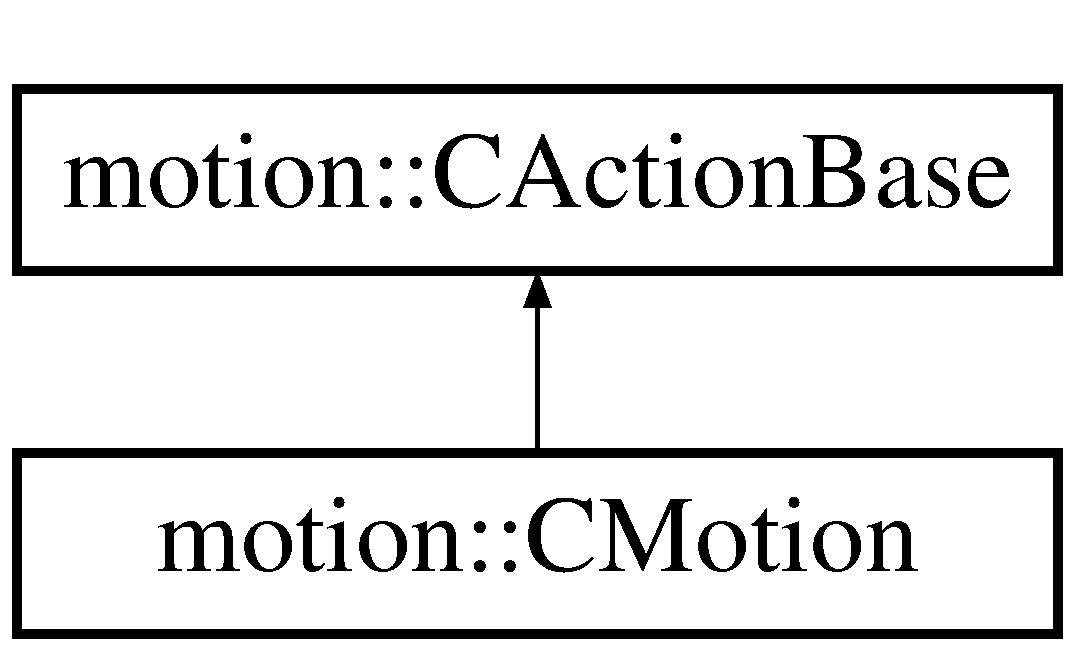
\includegraphics[height=2.000000cm]{classmotion_1_1CMotion}
\end{center}
\end{figure}
\subsection*{Public Member Functions}
\begin{DoxyCompactItemize}
\item 
void \mbox{\hyperlink{classmotion_1_1CMotion_a7e4c27c99fca247140ff23e693be7e7a}{update}} (void)
\item 
\mbox{\Hypertarget{classmotion_1_1CMotion_a95a158cf97317b99f614c726b398ff9e}\label{classmotion_1_1CMotion_a95a158cf97317b99f614c726b398ff9e}} 
void {\bfseries reset} (void)
\item 
\mbox{\Hypertarget{classmotion_1_1CMotion_a502c2ceefa31655ac88c786a969525ab}\label{classmotion_1_1CMotion_a502c2ceefa31655ac88c786a969525ab}} 
\mbox{\hyperlink{classmotion_1_1CStateMachine}{C\+State\+Machine}}$<$ \mbox{\hyperlink{classmotion_1_1CMotion}{C\+Motion}} $>$ $\ast$ {\bfseries get\+F\+SM} (void) const
\end{DoxyCompactItemize}
\subsection*{Static Public Member Functions}
\begin{DoxyCompactItemize}
\item 
\mbox{\Hypertarget{classmotion_1_1CMotion_ae4f9348f30ec8f233053761695adb5f6}\label{classmotion_1_1CMotion_ae4f9348f30ec8f233053761695adb5f6}} 
static \mbox{\hyperlink{classmotion_1_1CMotion}{C\+Motion}} $\ast$ {\bfseries get\+Instance} (void)
\end{DoxyCompactItemize}


\subsection{Detailed Description}
Motion ~\newline
 example\+: ~\newline
 //to update motion mtn-\/$>$\mbox{\hyperlink{classmotion_1_1CMotion_a7e4c27c99fca247140ff23e693be7e7a}{update()}}; ~\newline


\subsection{Member Function Documentation}
\mbox{\Hypertarget{classmotion_1_1CMotion_a7e4c27c99fca247140ff23e693be7e7a}\label{classmotion_1_1CMotion_a7e4c27c99fca247140ff23e693be7e7a}} 
\index{motion\+::\+C\+Motion@{motion\+::\+C\+Motion}!update@{update}}
\index{update@{update}!motion\+::\+C\+Motion@{motion\+::\+C\+Motion}}
\subsubsection{\texorpdfstring{update()}{update()}}
{\footnotesize\ttfamily void C\+Motion\+::update (\begin{DoxyParamCaption}\item[{void}]{ }\end{DoxyParamCaption})}

Check bump and lift later here. 

The documentation for this class was generated from the following files\+:\begin{DoxyCompactItemize}
\item 
motion/\mbox{\hyperlink{CMotion_8h}{C\+Motion.\+h}}\item 
motion/\mbox{\hyperlink{CMotion_8cpp}{C\+Motion.\+cpp}}\end{DoxyCompactItemize}

\hypertarget{classmotion_1_1CMotionIdle}{}\section{motion\+:\+:C\+Motion\+Idle Class Reference}
\label{classmotion_1_1CMotionIdle}\index{motion\+::\+C\+Motion\+Idle@{motion\+::\+C\+Motion\+Idle}}


{\ttfamily \#include $<$C\+Motion\+Idle.\+h$>$}

Inheritance diagram for motion\+:\+:C\+Motion\+Idle\+:\begin{figure}[H]
\begin{center}
\leavevmode
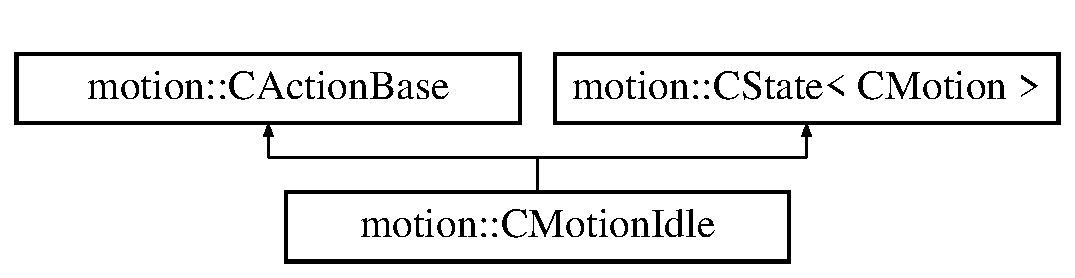
\includegraphics[height=2.000000cm]{classmotion_1_1CMotionIdle}
\end{center}
\end{figure}
\subsection*{Public Member Functions}
\begin{DoxyCompactItemize}
\item 
virtual \mbox{\hyperlink{classmotion_1_1CMotionIdle_a45b57a25a1b53c585fc2ef648dc1ec4a}{$\sim$\+C\+Motion\+Idle}} (void)
\item 
virtual void \mbox{\hyperlink{classmotion_1_1CMotionIdle_adf54cf3d93e54060a3060017e55ea706}{enter}} (\mbox{\hyperlink{classmotion_1_1CMotion}{C\+Motion}} $\ast$mt)
\item 
virtual void \mbox{\hyperlink{classmotion_1_1CMotionIdle_aad314bae00925e2fdbbf8e93fff08b9a}{execute}} (\mbox{\hyperlink{classmotion_1_1CMotion}{C\+Motion}} $\ast$mt)
\item 
virtual void \mbox{\hyperlink{classmotion_1_1CMotionIdle_a2488eb5516673fd8e188da01a9e4bc51}{exit}} (\mbox{\hyperlink{classmotion_1_1CMotion}{C\+Motion}} $\ast$mt)
\end{DoxyCompactItemize}
\subsection*{Static Public Member Functions}
\begin{DoxyCompactItemize}
\item 
\mbox{\Hypertarget{classmotion_1_1CMotionIdle_acbd0fc59cc7ee93ec4a13049d7e1f419}\label{classmotion_1_1CMotionIdle_acbd0fc59cc7ee93ec4a13049d7e1f419}} 
static \mbox{\hyperlink{classmotion_1_1CMotionIdle}{C\+Motion\+Idle}} $\ast$ {\bfseries get\+Instance} (void)
\end{DoxyCompactItemize}


\subsection{Detailed Description}
Motion idle state ~\newline
 example\+: ~\newline
// To change to this state from other state ~\newline
 \#include \mbox{\hyperlink{CMotion_8h}{C\+Motion.\+h}} ~\newline
 mtn-\/$>$set\+Motion(\+M\+O\+T\+I\+O\+N\+\_\+\+I\+D\+L\+E); ~\newline


\subsection{Constructor \& Destructor Documentation}
\mbox{\Hypertarget{classmotion_1_1CMotionIdle_a45b57a25a1b53c585fc2ef648dc1ec4a}\label{classmotion_1_1CMotionIdle_a45b57a25a1b53c585fc2ef648dc1ec4a}} 
\index{motion\+::\+C\+Motion\+Idle@{motion\+::\+C\+Motion\+Idle}!````~C\+Motion\+Idle@{$\sim$\+C\+Motion\+Idle}}
\index{````~C\+Motion\+Idle@{$\sim$\+C\+Motion\+Idle}!motion\+::\+C\+Motion\+Idle@{motion\+::\+C\+Motion\+Idle}}
\subsubsection{\texorpdfstring{$\sim$\+C\+Motion\+Idle()}{~CMotionIdle()}}
{\footnotesize\ttfamily virtual motion\+::\+C\+Motion\+Idle\+::$\sim$\+C\+Motion\+Idle (\begin{DoxyParamCaption}\item[{void}]{ }\end{DoxyParamCaption})\hspace{0.3cm}{\ttfamily [inline]}, {\ttfamily [virtual]}}

delete m\+\_\+p\+State\+Machine; 

\subsection{Member Function Documentation}
\mbox{\Hypertarget{classmotion_1_1CMotionIdle_adf54cf3d93e54060a3060017e55ea706}\label{classmotion_1_1CMotionIdle_adf54cf3d93e54060a3060017e55ea706}} 
\index{motion\+::\+C\+Motion\+Idle@{motion\+::\+C\+Motion\+Idle}!enter@{enter}}
\index{enter@{enter}!motion\+::\+C\+Motion\+Idle@{motion\+::\+C\+Motion\+Idle}}
\subsubsection{\texorpdfstring{enter()}{enter()}}
{\footnotesize\ttfamily void C\+Motion\+Idle\+::enter (\begin{DoxyParamCaption}\item[{\mbox{\hyperlink{classmotion_1_1CMotion}{C\+Motion}} $\ast$}]{ }\end{DoxyParamCaption})\hspace{0.3cm}{\ttfamily [virtual]}}

This will execute when the state is entered. 

Implements \mbox{\hyperlink{classmotion_1_1CState_a53d5fcfec223b58ccdd364a8430fd23c}{motion\+::\+C\+State$<$ C\+Motion $>$}}.

\mbox{\Hypertarget{classmotion_1_1CMotionIdle_aad314bae00925e2fdbbf8e93fff08b9a}\label{classmotion_1_1CMotionIdle_aad314bae00925e2fdbbf8e93fff08b9a}} 
\index{motion\+::\+C\+Motion\+Idle@{motion\+::\+C\+Motion\+Idle}!execute@{execute}}
\index{execute@{execute}!motion\+::\+C\+Motion\+Idle@{motion\+::\+C\+Motion\+Idle}}
\subsubsection{\texorpdfstring{execute()}{execute()}}
{\footnotesize\ttfamily void C\+Motion\+Idle\+::execute (\begin{DoxyParamCaption}\item[{\mbox{\hyperlink{classmotion_1_1CMotion}{C\+Motion}} $\ast$}]{ }\end{DoxyParamCaption})\hspace{0.3cm}{\ttfamily [virtual]}}

This is the states normal update function. 

Implements \mbox{\hyperlink{classmotion_1_1CState_a71dc72d345b15bf3b5b5bff596a71f33}{motion\+::\+C\+State$<$ C\+Motion $>$}}.

\mbox{\Hypertarget{classmotion_1_1CMotionIdle_a2488eb5516673fd8e188da01a9e4bc51}\label{classmotion_1_1CMotionIdle_a2488eb5516673fd8e188da01a9e4bc51}} 
\index{motion\+::\+C\+Motion\+Idle@{motion\+::\+C\+Motion\+Idle}!exit@{exit}}
\index{exit@{exit}!motion\+::\+C\+Motion\+Idle@{motion\+::\+C\+Motion\+Idle}}
\subsubsection{\texorpdfstring{exit()}{exit()}}
{\footnotesize\ttfamily void C\+Motion\+Idle\+::exit (\begin{DoxyParamCaption}\item[{\mbox{\hyperlink{classmotion_1_1CMotion}{C\+Motion}} $\ast$}]{ }\end{DoxyParamCaption})\hspace{0.3cm}{\ttfamily [virtual]}}

This will execute when the state is exited. 

Implements \mbox{\hyperlink{classmotion_1_1CState_a353db064c159d66b82bf257b35e7c016}{motion\+::\+C\+State$<$ C\+Motion $>$}}.



The documentation for this class was generated from the following files\+:\begin{DoxyCompactItemize}
\item 
motion/\mbox{\hyperlink{CMotionIdle_8h}{C\+Motion\+Idle.\+h}}\item 
motion/\mbox{\hyperlink{CMotionIdle_8cpp}{C\+Motion\+Idle.\+cpp}}\end{DoxyCompactItemize}

\hypertarget{classmotion_1_1CMotionPointTracker}{}\section{motion\+:\+:C\+Motion\+Point\+Tracker Class Reference}
\label{classmotion_1_1CMotionPointTracker}\index{motion\+::\+C\+Motion\+Point\+Tracker@{motion\+::\+C\+Motion\+Point\+Tracker}}


{\ttfamily \#include $<$C\+Motion\+Point\+Tracker.\+h$>$}

Inheritance diagram for motion\+:\+:C\+Motion\+Point\+Tracker\+:\begin{figure}[H]
\begin{center}
\leavevmode
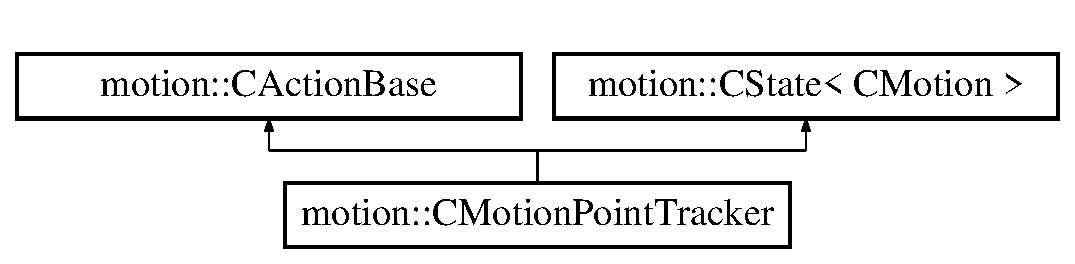
\includegraphics[height=2.000000cm]{classmotion_1_1CMotionPointTracker}
\end{center}
\end{figure}
\subsection*{Public Member Functions}
\begin{DoxyCompactItemize}
\item 
virtual void \mbox{\hyperlink{classmotion_1_1CMotionPointTracker_a77975b88cc198d7115910dd0e738f925}{enter}} (\mbox{\hyperlink{classmotion_1_1CMotion}{C\+Motion}} $\ast$mt)
\item 
virtual void \mbox{\hyperlink{classmotion_1_1CMotionPointTracker_a2513b0d052536d307db674af8ee8a3e6}{execute}} (\mbox{\hyperlink{classmotion_1_1CMotion}{C\+Motion}} $\ast$mt)
\item 
virtual void \mbox{\hyperlink{classmotion_1_1CMotionPointTracker_ae40c6dc8e2883a6293b2ea5994b0e3d1}{exit}} (\mbox{\hyperlink{classmotion_1_1CMotion}{C\+Motion}} $\ast$mt)
\item 
\mbox{\Hypertarget{classmotion_1_1CMotionPointTracker_a6a3e63319c5059316543779904495599}\label{classmotion_1_1CMotionPointTracker_a6a3e63319c5059316543779904495599}} 
void {\bfseries reset} (void)
\item 
\mbox{\Hypertarget{classmotion_1_1CMotionPointTracker_a2532e7afbf434af45d8cfa75551fde47}\label{classmotion_1_1CMotionPointTracker_a2532e7afbf434af45d8cfa75551fde47}} 
int {\bfseries arc\+Side} (void)
\item 
\mbox{\Hypertarget{classmotion_1_1CMotionPointTracker_add639f835d6ac5c35c84d0768a574c7c}\label{classmotion_1_1CMotionPointTracker_add639f835d6ac5c35c84d0768a574c7c}} 
double {\bfseries get\+Dist} (void) const
\item 
\mbox{\Hypertarget{classmotion_1_1CMotionPointTracker_a5b074c876ffd5432449ebaecc47fcc57}\label{classmotion_1_1CMotionPointTracker_a5b074c876ffd5432449ebaecc47fcc57}} 
\mbox{\hyperlink{motionEnums_8h_a5a442990f649a5e91cbd8205f16dabfc}{E\+Linear\+P\+T\+State}} {\bfseries getlpt\+State} (void) const
\item 
\mbox{\Hypertarget{classmotion_1_1CMotionPointTracker_a94eb508c2a7f071d467b6ab91809dc8e}\label{classmotion_1_1CMotionPointTracker_a94eb508c2a7f071d467b6ab91809dc8e}} 
void {\bfseries setlpt\+State} (\mbox{\hyperlink{motionEnums_8h_a5a442990f649a5e91cbd8205f16dabfc}{E\+Linear\+P\+T\+State}} s)
\item 
\mbox{\Hypertarget{classmotion_1_1CMotionPointTracker_ab5044793c84311aa4d8bd5edd2e60d35}\label{classmotion_1_1CMotionPointTracker_ab5044793c84311aa4d8bd5edd2e60d35}} 
\mbox{\hyperlink{classmotion_1_1CStateMachine}{C\+State\+Machine}}$<$ \mbox{\hyperlink{classmotion_1_1CMotionPointTracker}{C\+Motion\+Point\+Tracker}} $>$ $\ast$ {\bfseries get\+F\+SM} (void) const
\item 
void \mbox{\hyperlink{classmotion_1_1CMotionPointTracker_ab8567bd6ad6c796d47e72cb633ee93d3}{calc\+Phi}} (void)
\item 
void \mbox{\hyperlink{classmotion_1_1CMotionPointTracker_abeaaec052308d9f7cab9d1fbb8db90c3}{calc\+Dist}} (void)
\item 
void \mbox{\hyperlink{classmotion_1_1CMotionPointTracker_a587b38d9065c24f76005adde9a21fb75}{turn2\+Targ\+Point}} (void)
\item 
void \mbox{\hyperlink{classmotion_1_1CMotionPointTracker_abde667e158fa615c6e761ac3167c9359}{track\+Point}} (void)
\item 
void \mbox{\hyperlink{classmotion_1_1CMotionPointTracker_a93fee9fef4b855533249ba19e428c306}{Arc\+PT}} (void)
\item 
void \mbox{\hyperlink{classmotion_1_1CMotionPointTracker_a79e987afad15936fb09e7e2705aff01e}{Linear\+PT}} (void)
\end{DoxyCompactItemize}
\subsection*{Static Public Member Functions}
\begin{DoxyCompactItemize}
\item 
\mbox{\Hypertarget{classmotion_1_1CMotionPointTracker_aaf797081d88b83b3af9acd23143fa7f5}\label{classmotion_1_1CMotionPointTracker_aaf797081d88b83b3af9acd23143fa7f5}} 
static \mbox{\hyperlink{classmotion_1_1CMotionPointTracker}{C\+Motion\+Point\+Tracker}} $\ast$ {\bfseries get\+Instance} (void)
\end{DoxyCompactItemize}


\subsection{Detailed Description}
Point tracking mode. need the target point and tracking mode as input. \begin{DoxySeeAlso}{See also}
E\+P\+T\+Mode 
\end{DoxySeeAlso}


\subsection{Member Function Documentation}
\mbox{\Hypertarget{classmotion_1_1CMotionPointTracker_a93fee9fef4b855533249ba19e428c306}\label{classmotion_1_1CMotionPointTracker_a93fee9fef4b855533249ba19e428c306}} 
\index{motion\+::\+C\+Motion\+Point\+Tracker@{motion\+::\+C\+Motion\+Point\+Tracker}!Arc\+PT@{Arc\+PT}}
\index{Arc\+PT@{Arc\+PT}!motion\+::\+C\+Motion\+Point\+Tracker@{motion\+::\+C\+Motion\+Point\+Tracker}}
\subsubsection{\texorpdfstring{Arc\+P\+T()}{ArcPT()}}
{\footnotesize\ttfamily void C\+Motion\+Point\+Tracker\+::\+Arc\+PT (\begin{DoxyParamCaption}\item[{void}]{ }\end{DoxyParamCaption})}

Arc point tracking method. todo \mbox{\Hypertarget{classmotion_1_1CMotionPointTracker_abeaaec052308d9f7cab9d1fbb8db90c3}\label{classmotion_1_1CMotionPointTracker_abeaaec052308d9f7cab9d1fbb8db90c3}} 
\index{motion\+::\+C\+Motion\+Point\+Tracker@{motion\+::\+C\+Motion\+Point\+Tracker}!calc\+Dist@{calc\+Dist}}
\index{calc\+Dist@{calc\+Dist}!motion\+::\+C\+Motion\+Point\+Tracker@{motion\+::\+C\+Motion\+Point\+Tracker}}
\subsubsection{\texorpdfstring{calc\+Dist()}{calcDist()}}
{\footnotesize\ttfamily void C\+Motion\+Point\+Tracker\+::calc\+Dist (\begin{DoxyParamCaption}\item[{void}]{ }\end{DoxyParamCaption})}

Calculate \begin{DoxySeeAlso}{See also}
m\+\_\+dist. 
\end{DoxySeeAlso}
printf(\char`\"{}\mbox{[}ljh\mbox{]} dist is\+: \%.\+3f\textbackslash{}n\char`\"{}, m\+\_\+dist); \mbox{\Hypertarget{classmotion_1_1CMotionPointTracker_ab8567bd6ad6c796d47e72cb633ee93d3}\label{classmotion_1_1CMotionPointTracker_ab8567bd6ad6c796d47e72cb633ee93d3}} 
\index{motion\+::\+C\+Motion\+Point\+Tracker@{motion\+::\+C\+Motion\+Point\+Tracker}!calc\+Phi@{calc\+Phi}}
\index{calc\+Phi@{calc\+Phi}!motion\+::\+C\+Motion\+Point\+Tracker@{motion\+::\+C\+Motion\+Point\+Tracker}}
\subsubsection{\texorpdfstring{calc\+Phi()}{calcPhi()}}
{\footnotesize\ttfamily void C\+Motion\+Point\+Tracker\+::calc\+Phi (\begin{DoxyParamCaption}\item[{void}]{ }\end{DoxyParamCaption})}

Calculate \begin{DoxySeeAlso}{See also}
m\+\_\+angle. 
\end{DoxySeeAlso}
double t\+Target\+Phi = atan2(vec\+Y, vec\+X); double t\+Angle\+Diff = get\+Cur\+Pose().phi -\/ t\+Target\+Phi; double t\+Nor\+Abs = motion\+Absd(normalize\+Theta(t\+Angle\+Diff)); ~\newline
~\newline
 printf(\char`\"{}angle is\+: \%.\+3f\textbackslash{}n\char`\"{}, angle); printf(\char`\"{}cphi\+: \%.\+3f\textbackslash{}n\char`\"{},get\+Cur\+Pose().phi); ~\newline
 printf(\char`\"{}tvect x\+: \%.\+3f, tvect y\+:\%.\+3f\textbackslash{}n\char`\"{}, vecX, vecY); printf(\char`\"{}cp\+: \%.\+3f\textbackslash{}n\char`\"{}, cross\+Prod); \mbox{\Hypertarget{classmotion_1_1CMotionPointTracker_a77975b88cc198d7115910dd0e738f925}\label{classmotion_1_1CMotionPointTracker_a77975b88cc198d7115910dd0e738f925}} 
\index{motion\+::\+C\+Motion\+Point\+Tracker@{motion\+::\+C\+Motion\+Point\+Tracker}!enter@{enter}}
\index{enter@{enter}!motion\+::\+C\+Motion\+Point\+Tracker@{motion\+::\+C\+Motion\+Point\+Tracker}}
\subsubsection{\texorpdfstring{enter()}{enter()}}
{\footnotesize\ttfamily void C\+Motion\+Point\+Tracker\+::enter (\begin{DoxyParamCaption}\item[{\mbox{\hyperlink{classmotion_1_1CMotion}{C\+Motion}} $\ast$}]{ }\end{DoxyParamCaption})\hspace{0.3cm}{\ttfamily [virtual]}}

This will execute when the state is entered. 

Implements \mbox{\hyperlink{classmotion_1_1CState_a53d5fcfec223b58ccdd364a8430fd23c}{motion\+::\+C\+State$<$ C\+Motion $>$}}.

\mbox{\Hypertarget{classmotion_1_1CMotionPointTracker_a2513b0d052536d307db674af8ee8a3e6}\label{classmotion_1_1CMotionPointTracker_a2513b0d052536d307db674af8ee8a3e6}} 
\index{motion\+::\+C\+Motion\+Point\+Tracker@{motion\+::\+C\+Motion\+Point\+Tracker}!execute@{execute}}
\index{execute@{execute}!motion\+::\+C\+Motion\+Point\+Tracker@{motion\+::\+C\+Motion\+Point\+Tracker}}
\subsubsection{\texorpdfstring{execute()}{execute()}}
{\footnotesize\ttfamily void C\+Motion\+Point\+Tracker\+::execute (\begin{DoxyParamCaption}\item[{\mbox{\hyperlink{classmotion_1_1CMotion}{C\+Motion}} $\ast$}]{ }\end{DoxyParamCaption})\hspace{0.3cm}{\ttfamily [virtual]}}

This is the states normal update function. 

Implements \mbox{\hyperlink{classmotion_1_1CState_a71dc72d345b15bf3b5b5bff596a71f33}{motion\+::\+C\+State$<$ C\+Motion $>$}}.

\mbox{\Hypertarget{classmotion_1_1CMotionPointTracker_ae40c6dc8e2883a6293b2ea5994b0e3d1}\label{classmotion_1_1CMotionPointTracker_ae40c6dc8e2883a6293b2ea5994b0e3d1}} 
\index{motion\+::\+C\+Motion\+Point\+Tracker@{motion\+::\+C\+Motion\+Point\+Tracker}!exit@{exit}}
\index{exit@{exit}!motion\+::\+C\+Motion\+Point\+Tracker@{motion\+::\+C\+Motion\+Point\+Tracker}}
\subsubsection{\texorpdfstring{exit()}{exit()}}
{\footnotesize\ttfamily void C\+Motion\+Point\+Tracker\+::exit (\begin{DoxyParamCaption}\item[{\mbox{\hyperlink{classmotion_1_1CMotion}{C\+Motion}} $\ast$}]{ }\end{DoxyParamCaption})\hspace{0.3cm}{\ttfamily [virtual]}}

This will execute when the state is exited. 

Implements \mbox{\hyperlink{classmotion_1_1CState_a353db064c159d66b82bf257b35e7c016}{motion\+::\+C\+State$<$ C\+Motion $>$}}.

\mbox{\Hypertarget{classmotion_1_1CMotionPointTracker_a79e987afad15936fb09e7e2705aff01e}\label{classmotion_1_1CMotionPointTracker_a79e987afad15936fb09e7e2705aff01e}} 
\index{motion\+::\+C\+Motion\+Point\+Tracker@{motion\+::\+C\+Motion\+Point\+Tracker}!Linear\+PT@{Linear\+PT}}
\index{Linear\+PT@{Linear\+PT}!motion\+::\+C\+Motion\+Point\+Tracker@{motion\+::\+C\+Motion\+Point\+Tracker}}
\subsubsection{\texorpdfstring{Linear\+P\+T()}{LinearPT()}}
{\footnotesize\ttfamily void C\+Motion\+Point\+Tracker\+::\+Linear\+PT (\begin{DoxyParamCaption}\item[{void}]{ }\end{DoxyParamCaption})}

Linear point tracking method. Rotate to the target direction. ~\newline
~\newline
 Forward with fixed v and calculated distance. ~\newline
 Replaced by change\+State(some\+Instance) later. todo \mbox{\Hypertarget{classmotion_1_1CMotionPointTracker_abde667e158fa615c6e761ac3167c9359}\label{classmotion_1_1CMotionPointTracker_abde667e158fa615c6e761ac3167c9359}} 
\index{motion\+::\+C\+Motion\+Point\+Tracker@{motion\+::\+C\+Motion\+Point\+Tracker}!track\+Point@{track\+Point}}
\index{track\+Point@{track\+Point}!motion\+::\+C\+Motion\+Point\+Tracker@{motion\+::\+C\+Motion\+Point\+Tracker}}
\subsubsection{\texorpdfstring{track\+Point()}{trackPoint()}}
{\footnotesize\ttfamily void C\+Motion\+Point\+Tracker\+::track\+Point (\begin{DoxyParamCaption}\item[{void}]{ }\end{DoxyParamCaption})}

Make the robot translate to the next point. todo \mbox{\Hypertarget{classmotion_1_1CMotionPointTracker_a587b38d9065c24f76005adde9a21fb75}\label{classmotion_1_1CMotionPointTracker_a587b38d9065c24f76005adde9a21fb75}} 
\index{motion\+::\+C\+Motion\+Point\+Tracker@{motion\+::\+C\+Motion\+Point\+Tracker}!turn2\+Targ\+Point@{turn2\+Targ\+Point}}
\index{turn2\+Targ\+Point@{turn2\+Targ\+Point}!motion\+::\+C\+Motion\+Point\+Tracker@{motion\+::\+C\+Motion\+Point\+Tracker}}
\subsubsection{\texorpdfstring{turn2\+Targ\+Point()}{turn2TargPoint()}}
{\footnotesize\ttfamily void C\+Motion\+Point\+Tracker\+::turn2\+Targ\+Point (\begin{DoxyParamCaption}\item[{void}]{ }\end{DoxyParamCaption})}

Make the robot turn to the next point. todo 

The documentation for this class was generated from the following files\+:\begin{DoxyCompactItemize}
\item 
motion/\mbox{\hyperlink{CMotionPointTracker_8h}{C\+Motion\+Point\+Tracker.\+h}}\item 
motion/\mbox{\hyperlink{CMotionPointTracker_8cpp}{C\+Motion\+Point\+Tracker.\+cpp}}\end{DoxyCompactItemize}

\hypertarget{classmotion_1_1CMotionWallFollowing}{}\section{motion\+:\+:C\+Motion\+Wall\+Following Class Reference}
\label{classmotion_1_1CMotionWallFollowing}\index{motion\+::\+C\+Motion\+Wall\+Following@{motion\+::\+C\+Motion\+Wall\+Following}}


{\ttfamily \#include $<$C\+Motion\+Wall\+Following.\+h$>$}

Inheritance diagram for motion\+:\+:C\+Motion\+Wall\+Following\+:\begin{figure}[H]
\begin{center}
\leavevmode
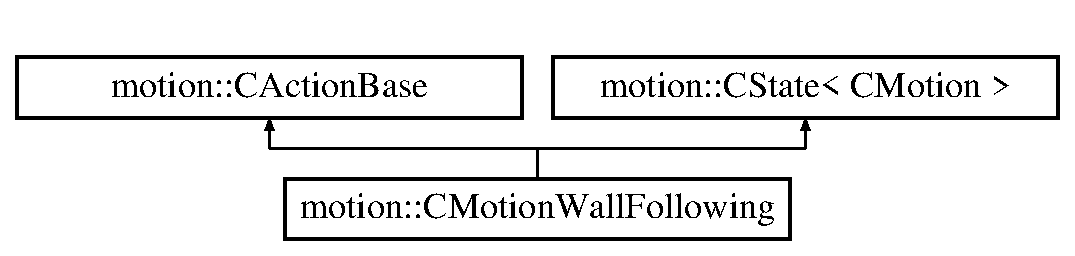
\includegraphics[height=2.000000cm]{classmotion_1_1CMotionWallFollowing}
\end{center}
\end{figure}
\subsection*{Public Member Functions}
\begin{DoxyCompactItemize}
\item 
virtual void \mbox{\hyperlink{classmotion_1_1CMotionWallFollowing_ad42584f648abe8826d2c23dad8128484}{enter}} (\mbox{\hyperlink{classmotion_1_1CMotion}{C\+Motion}} $\ast$mt)
\item 
virtual void \mbox{\hyperlink{classmotion_1_1CMotionWallFollowing_a765cfe604941a06056131feb01fea66d}{execute}} (\mbox{\hyperlink{classmotion_1_1CMotion}{C\+Motion}} $\ast$mt)
\item 
virtual void \mbox{\hyperlink{classmotion_1_1CMotionWallFollowing_a24be76c786b3a4bd476cc9b3c8955c26}{exit}} (\mbox{\hyperlink{classmotion_1_1CMotion}{C\+Motion}} $\ast$mt)
\item 
\mbox{\Hypertarget{classmotion_1_1CMotionWallFollowing_ab85ceaa8803a0850acdc951bd9ebec74}\label{classmotion_1_1CMotionWallFollowing_ab85ceaa8803a0850acdc951bd9ebec74}} 
void {\bfseries reset} (void)
\item 
\mbox{\Hypertarget{classmotion_1_1CMotionWallFollowing_a0ab894226ca05974580ec97ececbda5d}\label{classmotion_1_1CMotionWallFollowing_a0ab894226ca05974580ec97ececbda5d}} 
\mbox{\hyperlink{classmotion_1_1CStateMachine}{C\+State\+Machine}}$<$ \mbox{\hyperlink{classmotion_1_1CMotionWallFollowing}{C\+Motion\+Wall\+Following}} $>$ $\ast$ {\bfseries get\+F\+SM} (void) const
\item 
double \mbox{\hyperlink{classmotion_1_1CMotionWallFollowing_a1b29295eff775104bb16c110c3f8b81a}{tune\+Velocity}} (void)
\item 
double \mbox{\hyperlink{classmotion_1_1CMotionWallFollowing_ad8a39e0176c9e6127b8267b1a7a891ac}{calc\+Rem\+Angle}} (void)
\item 
bool \mbox{\hyperlink{classmotion_1_1CMotionWallFollowing_a4fcea1525cdd043f8c0dd8621e3ba09e}{dist\+Reached}} (void)
\item 
bool \mbox{\hyperlink{classmotion_1_1CMotionWallFollowing_aa84fb18a4cea89ad726c18d4f308e4d7}{ang\+N\+Dist\+Reached}} (void)
\end{DoxyCompactItemize}
\subsection*{Static Public Member Functions}
\begin{DoxyCompactItemize}
\item 
\mbox{\Hypertarget{classmotion_1_1CMotionWallFollowing_a8758349202ccb49d5b0927066b4201cd}\label{classmotion_1_1CMotionWallFollowing_a8758349202ccb49d5b0927066b4201cd}} 
static \mbox{\hyperlink{classmotion_1_1CMotionWallFollowing}{C\+Motion\+Wall\+Following}} $\ast$ {\bfseries get\+Instance} (void)
\end{DoxyCompactItemize}


\subsection{Detailed Description}
Wall following mode. Need the following linear velocity and the desired follow distance as input. 

\subsection{Member Function Documentation}
\mbox{\Hypertarget{classmotion_1_1CMotionWallFollowing_aa84fb18a4cea89ad726c18d4f308e4d7}\label{classmotion_1_1CMotionWallFollowing_aa84fb18a4cea89ad726c18d4f308e4d7}} 
\index{motion\+::\+C\+Motion\+Wall\+Following@{motion\+::\+C\+Motion\+Wall\+Following}!ang\+N\+Dist\+Reached@{ang\+N\+Dist\+Reached}}
\index{ang\+N\+Dist\+Reached@{ang\+N\+Dist\+Reached}!motion\+::\+C\+Motion\+Wall\+Following@{motion\+::\+C\+Motion\+Wall\+Following}}
\subsubsection{\texorpdfstring{ang\+N\+Dist\+Reached()}{angNDistReached()}}
{\footnotesize\ttfamily bool C\+Motion\+Wall\+Following\+::ang\+N\+Dist\+Reached (\begin{DoxyParamCaption}\item[{void}]{ }\end{DoxyParamCaption})}

The resume angle and distance satisfied or not. \begin{DoxyReturn}{Returns}
true if angle condition is satisfied and side distance is larger than obs\+Stop\+Dist. 
\end{DoxyReturn}
\begin{DoxySeeAlso}{See also}
\mbox{\hyperlink{classmotion_1_1CMotionWallFollowing_a4fcea1525cdd043f8c0dd8621e3ba09e}{dist\+Reached}} 

obs\+Stop\+Dist 
\end{DoxySeeAlso}
\mbox{\Hypertarget{classmotion_1_1CMotionWallFollowing_ad8a39e0176c9e6127b8267b1a7a891ac}\label{classmotion_1_1CMotionWallFollowing_ad8a39e0176c9e6127b8267b1a7a891ac}} 
\index{motion\+::\+C\+Motion\+Wall\+Following@{motion\+::\+C\+Motion\+Wall\+Following}!calc\+Rem\+Angle@{calc\+Rem\+Angle}}
\index{calc\+Rem\+Angle@{calc\+Rem\+Angle}!motion\+::\+C\+Motion\+Wall\+Following@{motion\+::\+C\+Motion\+Wall\+Following}}
\subsubsection{\texorpdfstring{calc\+Rem\+Angle()}{calcRemAngle()}}
{\footnotesize\ttfamily double C\+Motion\+Wall\+Following\+::calc\+Rem\+Angle (\begin{DoxyParamCaption}\item[{void}]{ }\end{DoxyParamCaption})}

Calculate remaining angle, when this angle approached 0, it means the angle condition of ang\+N\+Dist\+Reached is satisfied. \begin{DoxyReturn}{Returns}
Remaining angle. 
\end{DoxyReturn}
\begin{DoxySeeAlso}{See also}
\mbox{\hyperlink{classmotion_1_1CMotionWallFollowing_aa84fb18a4cea89ad726c18d4f308e4d7}{ang\+N\+Dist\+Reached}} 
\end{DoxySeeAlso}
return motion\+Absd(rad2\+Deg(m\+\_\+end\+Phi -\/ get\+Cur\+Pose().phi)); \mbox{\Hypertarget{classmotion_1_1CMotionWallFollowing_a4fcea1525cdd043f8c0dd8621e3ba09e}\label{classmotion_1_1CMotionWallFollowing_a4fcea1525cdd043f8c0dd8621e3ba09e}} 
\index{motion\+::\+C\+Motion\+Wall\+Following@{motion\+::\+C\+Motion\+Wall\+Following}!dist\+Reached@{dist\+Reached}}
\index{dist\+Reached@{dist\+Reached}!motion\+::\+C\+Motion\+Wall\+Following@{motion\+::\+C\+Motion\+Wall\+Following}}
\subsubsection{\texorpdfstring{dist\+Reached()}{distReached()}}
{\footnotesize\ttfamily bool C\+Motion\+Wall\+Following\+::dist\+Reached (\begin{DoxyParamCaption}\item[{void}]{ }\end{DoxyParamCaption})}

The resume distance satisfied or not. \begin{DoxyReturn}{Returns}
true if ahead distance is larger than wall\+Fol\+Resume\+Dist. 
\end{DoxyReturn}
\begin{DoxySeeAlso}{See also}
\mbox{\hyperlink{classmotion_1_1CMotionWallFollowing_aa84fb18a4cea89ad726c18d4f308e4d7}{ang\+N\+Dist\+Reached}} 

wall\+Fol\+Resume\+Dist 
\end{DoxySeeAlso}
\mbox{\Hypertarget{classmotion_1_1CMotionWallFollowing_ad42584f648abe8826d2c23dad8128484}\label{classmotion_1_1CMotionWallFollowing_ad42584f648abe8826d2c23dad8128484}} 
\index{motion\+::\+C\+Motion\+Wall\+Following@{motion\+::\+C\+Motion\+Wall\+Following}!enter@{enter}}
\index{enter@{enter}!motion\+::\+C\+Motion\+Wall\+Following@{motion\+::\+C\+Motion\+Wall\+Following}}
\subsubsection{\texorpdfstring{enter()}{enter()}}
{\footnotesize\ttfamily void C\+Motion\+Wall\+Following\+::enter (\begin{DoxyParamCaption}\item[{\mbox{\hyperlink{classmotion_1_1CMotion}{C\+Motion}} $\ast$}]{ }\end{DoxyParamCaption})\hspace{0.3cm}{\ttfamily [virtual]}}

This will execute when the state is entered. set\+Motion(\+W\+A\+L\+L\+\_\+\+F\+O\+L\+L\+O\+W\+I\+N\+G); 

Implements \mbox{\hyperlink{classmotion_1_1CState_a53d5fcfec223b58ccdd364a8430fd23c}{motion\+::\+C\+State$<$ C\+Motion $>$}}.

\mbox{\Hypertarget{classmotion_1_1CMotionWallFollowing_a765cfe604941a06056131feb01fea66d}\label{classmotion_1_1CMotionWallFollowing_a765cfe604941a06056131feb01fea66d}} 
\index{motion\+::\+C\+Motion\+Wall\+Following@{motion\+::\+C\+Motion\+Wall\+Following}!execute@{execute}}
\index{execute@{execute}!motion\+::\+C\+Motion\+Wall\+Following@{motion\+::\+C\+Motion\+Wall\+Following}}
\subsubsection{\texorpdfstring{execute()}{execute()}}
{\footnotesize\ttfamily void C\+Motion\+Wall\+Following\+::execute (\begin{DoxyParamCaption}\item[{\mbox{\hyperlink{classmotion_1_1CMotion}{C\+Motion}} $\ast$}]{ }\end{DoxyParamCaption})\hspace{0.3cm}{\ttfamily [virtual]}}

This is the states normal update function. 

Implements \mbox{\hyperlink{classmotion_1_1CState_a71dc72d345b15bf3b5b5bff596a71f33}{motion\+::\+C\+State$<$ C\+Motion $>$}}.

\mbox{\Hypertarget{classmotion_1_1CMotionWallFollowing_a24be76c786b3a4bd476cc9b3c8955c26}\label{classmotion_1_1CMotionWallFollowing_a24be76c786b3a4bd476cc9b3c8955c26}} 
\index{motion\+::\+C\+Motion\+Wall\+Following@{motion\+::\+C\+Motion\+Wall\+Following}!exit@{exit}}
\index{exit@{exit}!motion\+::\+C\+Motion\+Wall\+Following@{motion\+::\+C\+Motion\+Wall\+Following}}
\subsubsection{\texorpdfstring{exit()}{exit()}}
{\footnotesize\ttfamily void C\+Motion\+Wall\+Following\+::exit (\begin{DoxyParamCaption}\item[{\mbox{\hyperlink{classmotion_1_1CMotion}{C\+Motion}} $\ast$}]{ }\end{DoxyParamCaption})\hspace{0.3cm}{\ttfamily [virtual]}}

This will execute when the state is exited. 

Implements \mbox{\hyperlink{classmotion_1_1CState_a353db064c159d66b82bf257b35e7c016}{motion\+::\+C\+State$<$ C\+Motion $>$}}.

\mbox{\Hypertarget{classmotion_1_1CMotionWallFollowing_a1b29295eff775104bb16c110c3f8b81a}\label{classmotion_1_1CMotionWallFollowing_a1b29295eff775104bb16c110c3f8b81a}} 
\index{motion\+::\+C\+Motion\+Wall\+Following@{motion\+::\+C\+Motion\+Wall\+Following}!tune\+Velocity@{tune\+Velocity}}
\index{tune\+Velocity@{tune\+Velocity}!motion\+::\+C\+Motion\+Wall\+Following@{motion\+::\+C\+Motion\+Wall\+Following}}
\subsubsection{\texorpdfstring{tune\+Velocity()}{tuneVelocity()}}
{\footnotesize\ttfamily double C\+Motion\+Wall\+Following\+::tune\+Velocity (\begin{DoxyParamCaption}\item[{void}]{ }\end{DoxyParamCaption})}

Tune the velocity according to the distance from robot to wall. \begin{DoxyReturn}{Returns}
The scale that velocity should be Tuned. It\textquotesingle{}s a ratio between 0 and 1. 
\end{DoxyReturn}


The documentation for this class was generated from the following files\+:\begin{DoxyCompactItemize}
\item 
motion/\mbox{\hyperlink{CMotionWallFollowing_8h}{C\+Motion\+Wall\+Following.\+h}}\item 
motion/\mbox{\hyperlink{CMotionWallFollowing_8cpp}{C\+Motion\+Wall\+Following.\+cpp}}\end{DoxyCompactItemize}

\hypertarget{classCMyGLCanvas}{}\section{C\+My\+G\+L\+Canvas Class Reference}
\label{classCMyGLCanvas}\index{C\+My\+G\+L\+Canvas@{C\+My\+G\+L\+Canvas}}
Inheritance diagram for C\+My\+G\+L\+Canvas\+:\begin{figure}[H]
\begin{center}
\leavevmode
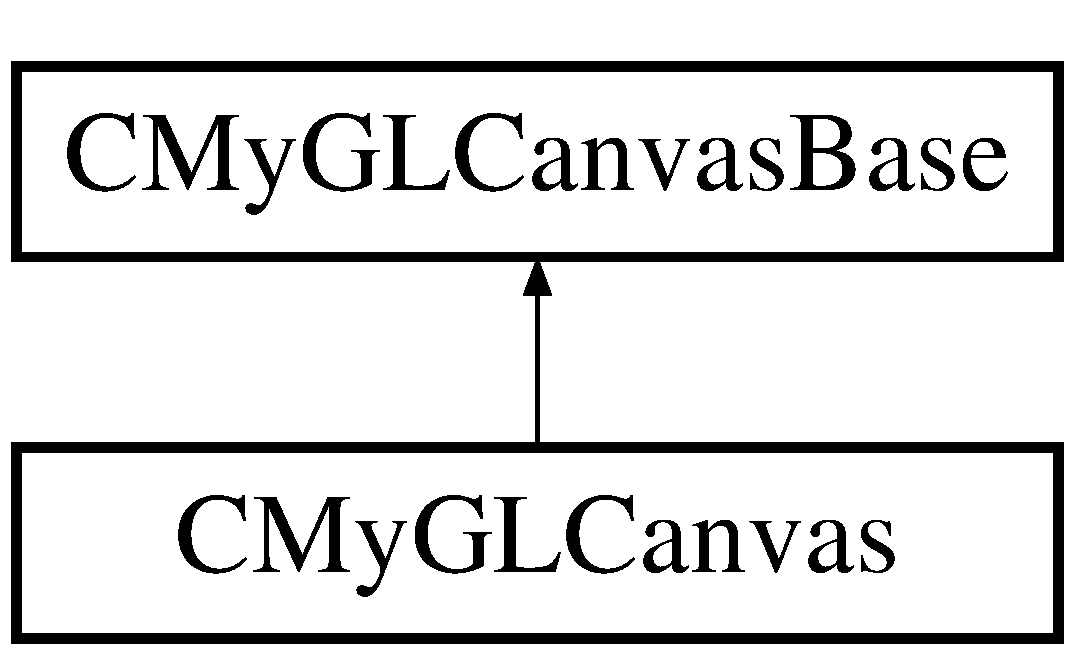
\includegraphics[height=2.000000cm]{classCMyGLCanvas}
\end{center}
\end{figure}
\subsection*{Public Member Functions}
\begin{DoxyCompactItemize}
\item 
\mbox{\Hypertarget{classCMyGLCanvas_a2444e5482d703a8d81d138cd2fb5d275}\label{classCMyGLCanvas_a2444e5482d703a8d81d138cd2fb5d275}} 
{\bfseries C\+My\+G\+L\+Canvas} (wx\+Window $\ast$parent, wx\+Window\+ID id=wx\+I\+D\+\_\+\+A\+NY, const wx\+Point \&pos=wx\+Default\+Position, const wx\+Size \&size=wx\+Default\+Size, long style=0, const wx\+String \&name=\+\_\+T(\char`\"{}C\+My\+G\+L\+Canvas\+Base\char`\"{}))
\item 
\mbox{\Hypertarget{classCMyGLCanvas_a136b603a8e7561bbdf15085daf349687}\label{classCMyGLCanvas_a136b603a8e7561bbdf15085daf349687}} 
void {\bfseries On\+Char\+Custom} (wx\+Key\+Event \&event)
\item 
\mbox{\Hypertarget{classCMyGLCanvas_a99b67a508a8603e6c5cf0856e9353bf6}\label{classCMyGLCanvas_a99b67a508a8603e6c5cf0856e9353bf6}} 
void {\bfseries On\+Pre\+Render} ()
\item 
\mbox{\Hypertarget{classCMyGLCanvas_aef8ded22cd9ecac73ad52c0ac6af46e1}\label{classCMyGLCanvas_aef8ded22cd9ecac73ad52c0ac6af46e1}} 
void {\bfseries On\+Post\+Render} ()
\item 
\mbox{\Hypertarget{classCMyGLCanvas_a4be08ca79a2f75ee1a142f136307dc57}\label{classCMyGLCanvas_a4be08ca79a2f75ee1a142f136307dc57}} 
void {\bfseries On\+Post\+Render\+Swap\+Buffers} (double At, wx\+Paint\+DC \&dc)
\item 
\mbox{\Hypertarget{classCMyGLCanvas_a33d6dfb37f2d4f11237a3c547d683047}\label{classCMyGLCanvas_a33d6dfb37f2d4f11237a3c547d683047}} 
void {\bfseries On\+Render\+Error} (const wx\+String \&str)
\end{DoxyCompactItemize}


The documentation for this class was generated from the following file\+:\begin{DoxyCompactItemize}
\item 
gridmap\+Simul\+Main.\+cpp\end{DoxyCompactItemize}

\hypertarget{classmotion_1_1CPathGenerator}{}\section{motion\+:\+:C\+Path\+Generator Class Reference}
\label{classmotion_1_1CPathGenerator}\index{motion\+::\+C\+Path\+Generator@{motion\+::\+C\+Path\+Generator}}


{\ttfamily \#include $<$C\+Path\+Generator.\+h$>$}

\subsection*{Public Member Functions}
\begin{DoxyCompactItemize}
\item 
list$<$ \mbox{\hyperlink{structmotion_1_1TMotionPoint}{T\+Motion\+Point}} $\ast$ $>$ \mbox{\hyperlink{classmotion_1_1CPathGenerator_ac9d9f955ec67e1d4abdcffd7b1fbecf5}{calc\+Path}} (\mbox{\hyperlink{structmotion_1_1TMotionPoint}{T\+Motion\+Point}} $\ast$start, \mbox{\hyperlink{structmotion_1_1TMotionPoint}{T\+Motion\+Point}} $\ast$target, bool is\+Ignore\+Corner)
\item 
vector$<$ \mbox{\hyperlink{structmotion_1_1TMotionPoint}{T\+Motion\+Point}} $\ast$ $>$ \mbox{\hyperlink{classmotion_1_1CPathGenerator_a58b067dca5c18f58fb2338d09b5075c6}{surrounding}} (\mbox{\hyperlink{structmotion_1_1TMotionPoint}{T\+Motion\+Point}} $\ast$cur\+Point, bool is\+Ignore\+Corner)
\item 
void \mbox{\hyperlink{classmotion_1_1CPathGenerator_af5b887f515f71346037e247c3171c147}{found\+Point}} (\mbox{\hyperlink{structmotion_1_1TMotionPoint}{T\+Motion\+Point}} $\ast$tmp\+Start\+Point, \mbox{\hyperlink{structmotion_1_1TMotionPoint}{T\+Motion\+Point}} $\ast$cur\+Point)
\item 
void \mbox{\hyperlink{classmotion_1_1CPathGenerator_a8756dcc952626706d20a7c9f8e4bfe8f}{not\+Found\+Point}} (\mbox{\hyperlink{structmotion_1_1TMotionPoint}{T\+Motion\+Point}} $\ast$tmp\+Start\+Point, \mbox{\hyperlink{structmotion_1_1TMotionPoint}{T\+Motion\+Point}} $\ast$target, \mbox{\hyperlink{structmotion_1_1TMotionPoint}{T\+Motion\+Point}} $\ast$cur\+Point)
\item 
bool \mbox{\hyperlink{classmotion_1_1CPathGenerator_ae2ede33b5f3dc5d9477ce7f0adf0ad89}{can\+Reach}} (\mbox{\hyperlink{structmotion_1_1TMotionPoint}{T\+Motion\+Point}} $\ast$cur\+Point, int x, int y, bool is\+Ignore\+Corner)
\item 
bool \mbox{\hyperlink{classmotion_1_1CPathGenerator_a7e940bbce29c6e35ac83dd87c6477574}{can\+Reach}} (int x, int y)
\item 
int \mbox{\hyperlink{classmotion_1_1CPathGenerator_acb04e6659d5b3b1a70c6cf485653d74e}{calcG}} (\mbox{\hyperlink{structmotion_1_1TMotionPoint}{T\+Motion\+Point}} $\ast$tmp\+Start\+Point, \mbox{\hyperlink{structmotion_1_1TMotionPoint}{T\+Motion\+Point}} $\ast$cur\+Point)
\item 
int \mbox{\hyperlink{classmotion_1_1CPathGenerator_a913cc37174472f68371bd4d3c6cca29a}{calcH}} (\mbox{\hyperlink{structmotion_1_1TMotionPoint}{T\+Motion\+Point}} $\ast$target, \mbox{\hyperlink{structmotion_1_1TMotionPoint}{T\+Motion\+Point}} $\ast$cur\+Point)
\item 
\mbox{\hyperlink{structmotion_1_1TMotionPoint}{T\+Motion\+Point}} $\ast$ \mbox{\hyperlink{classmotion_1_1CPathGenerator_a095212daf53fd9d74d94d638e10df03e}{find\+Min}} (void)
\item 
\mbox{\hyperlink{structmotion_1_1TMotionPoint}{T\+Motion\+Point}} $\ast$ \mbox{\hyperlink{classmotion_1_1CPathGenerator_a2ff43d2afeedcd679aca4795b193ef1b}{is\+Exist}} (list$<$ \mbox{\hyperlink{structmotion_1_1TMotionPoint}{T\+Motion\+Point}} $\ast$$>$ \&list, \mbox{\hyperlink{structmotion_1_1TMotionPoint}{T\+Motion\+Point}} $\ast$point)
\end{DoxyCompactItemize}


\subsection{Detailed Description}
Generate a path input\+: start point, end point, is\+Ignore\+Corner mark output\+: path(a list of point or N\+U\+L\+L) 

\subsection{Member Function Documentation}
\mbox{\Hypertarget{classmotion_1_1CPathGenerator_acb04e6659d5b3b1a70c6cf485653d74e}\label{classmotion_1_1CPathGenerator_acb04e6659d5b3b1a70c6cf485653d74e}} 
\index{motion\+::\+C\+Path\+Generator@{motion\+::\+C\+Path\+Generator}!calcG@{calcG}}
\index{calcG@{calcG}!motion\+::\+C\+Path\+Generator@{motion\+::\+C\+Path\+Generator}}
\subsubsection{\texorpdfstring{calc\+G()}{calcG()}}
{\footnotesize\ttfamily int C\+Path\+Generator\+::calcG (\begin{DoxyParamCaption}\item[{\mbox{\hyperlink{structmotion_1_1TMotionPoint}{T\+Motion\+Point}} $\ast$}]{tmp\+Start\+Point,  }\item[{\mbox{\hyperlink{structmotion_1_1TMotionPoint}{T\+Motion\+Point}} $\ast$}]{cur\+Point }\end{DoxyParamCaption})}

Calculate G value. 
\begin{DoxyParams}{Parameters}
{\em tmp\+Start\+Point} & The point in the center. \\
\hline
{\em cur\+Point} & Current point(it\textquotesingle{}s one of the surrounding points). \\
\hline
\end{DoxyParams}
\mbox{\Hypertarget{classmotion_1_1CPathGenerator_a913cc37174472f68371bd4d3c6cca29a}\label{classmotion_1_1CPathGenerator_a913cc37174472f68371bd4d3c6cca29a}} 
\index{motion\+::\+C\+Path\+Generator@{motion\+::\+C\+Path\+Generator}!calcH@{calcH}}
\index{calcH@{calcH}!motion\+::\+C\+Path\+Generator@{motion\+::\+C\+Path\+Generator}}
\subsubsection{\texorpdfstring{calc\+H()}{calcH()}}
{\footnotesize\ttfamily int C\+Path\+Generator\+::calcH (\begin{DoxyParamCaption}\item[{\mbox{\hyperlink{structmotion_1_1TMotionPoint}{T\+Motion\+Point}} $\ast$}]{target,  }\item[{\mbox{\hyperlink{structmotion_1_1TMotionPoint}{T\+Motion\+Point}} $\ast$}]{cur\+Point }\end{DoxyParamCaption})}

Calculate H value. 
\begin{DoxyParams}{Parameters}
{\em target} & The targe point. \\
\hline
{\em cur\+Point} & Current point(it\textquotesingle{}s one of the surrounding points). \\
\hline
\end{DoxyParams}
\mbox{\Hypertarget{classmotion_1_1CPathGenerator_ac9d9f955ec67e1d4abdcffd7b1fbecf5}\label{classmotion_1_1CPathGenerator_ac9d9f955ec67e1d4abdcffd7b1fbecf5}} 
\index{motion\+::\+C\+Path\+Generator@{motion\+::\+C\+Path\+Generator}!calc\+Path@{calc\+Path}}
\index{calc\+Path@{calc\+Path}!motion\+::\+C\+Path\+Generator@{motion\+::\+C\+Path\+Generator}}
\subsubsection{\texorpdfstring{calc\+Path()}{calcPath()}}
{\footnotesize\ttfamily list$<$ \mbox{\hyperlink{structmotion_1_1TMotionPoint}{T\+Motion\+Point}} $\ast$ $>$ C\+Path\+Generator\+::calc\+Path (\begin{DoxyParamCaption}\item[{\mbox{\hyperlink{structmotion_1_1TMotionPoint}{T\+Motion\+Point}} $\ast$}]{start,  }\item[{\mbox{\hyperlink{structmotion_1_1TMotionPoint}{T\+Motion\+Point}} $\ast$}]{target,  }\item[{bool}]{is\+Ignore\+Corner }\end{DoxyParamCaption})}

Calculate the path from start point to target point. 
\begin{DoxyParams}{Parameters}
{\em start} & Start point. \\
\hline
{\em target} & Target point. \\
\hline
{\em is\+Ignore\+Corner} & Is ignore corner obstacle. \\
\hline
\end{DoxyParams}
\begin{DoxyReturn}{Returns}
point list which is exactly the path from start to target. N\+U\+LL if no path found. 
\end{DoxyReturn}
\mbox{\Hypertarget{classmotion_1_1CPathGenerator_ae2ede33b5f3dc5d9477ce7f0adf0ad89}\label{classmotion_1_1CPathGenerator_ae2ede33b5f3dc5d9477ce7f0adf0ad89}} 
\index{motion\+::\+C\+Path\+Generator@{motion\+::\+C\+Path\+Generator}!can\+Reach@{can\+Reach}}
\index{can\+Reach@{can\+Reach}!motion\+::\+C\+Path\+Generator@{motion\+::\+C\+Path\+Generator}}
\subsubsection{\texorpdfstring{can\+Reach()}{canReach()}\hspace{0.1cm}{\footnotesize\ttfamily [1/2]}}
{\footnotesize\ttfamily bool C\+Path\+Generator\+::can\+Reach (\begin{DoxyParamCaption}\item[{\mbox{\hyperlink{structmotion_1_1TMotionPoint}{T\+Motion\+Point}} $\ast$}]{cur\+Point,  }\item[{int}]{x,  }\item[{int}]{y,  }\item[{bool}]{is\+Ignore\+Corner }\end{DoxyParamCaption})}

Is the given point reachable. 
\begin{DoxyParams}{Parameters}
{\em cur\+Point} & Current point. \\
\hline
{\em x} & x axis of the point evaluated. \\
\hline
{\em y} & y axis of the point evaluated. \\
\hline
{\em is\+Ignore\+Corner} & Is ignore corner obstacle. \\
\hline
\end{DoxyParams}
\begin{DoxyReturn}{Returns}
A vector that contains all of the surrounding points of current point. 
\end{DoxyReturn}
\begin{DoxySeeAlso}{See also}
\mbox{\hyperlink{classmotion_1_1CPathGenerator_ae2ede33b5f3dc5d9477ce7f0adf0ad89}{can\+Reach}} 

\mbox{\hyperlink{classmotion_1_1CPathGenerator_a58b067dca5c18f58fb2338d09b5075c6}{surrounding}} 
\end{DoxySeeAlso}
�� 1 ���Ҳ���close\+List

x y�����ϡ��¡����� \mbox{\Hypertarget{classmotion_1_1CPathGenerator_a7e940bbce29c6e35ac83dd87c6477574}\label{classmotion_1_1CPathGenerator_a7e940bbce29c6e35ac83dd87c6477574}} 
\index{motion\+::\+C\+Path\+Generator@{motion\+::\+C\+Path\+Generator}!can\+Reach@{can\+Reach}}
\index{can\+Reach@{can\+Reach}!motion\+::\+C\+Path\+Generator@{motion\+::\+C\+Path\+Generator}}
\subsubsection{\texorpdfstring{can\+Reach()}{canReach()}\hspace{0.1cm}{\footnotesize\ttfamily [2/2]}}
{\footnotesize\ttfamily bool C\+Path\+Generator\+::can\+Reach (\begin{DoxyParamCaption}\item[{int}]{x,  }\item[{int}]{y }\end{DoxyParamCaption})}

Is the given point reachable. 
\begin{DoxyParams}{Parameters}
{\em x} & x axis of the point evaluated. \\
\hline
{\em y} & y axis of the point evaluated. \\
\hline
\end{DoxyParams}
\mbox{\Hypertarget{classmotion_1_1CPathGenerator_a095212daf53fd9d74d94d638e10df03e}\label{classmotion_1_1CPathGenerator_a095212daf53fd9d74d94d638e10df03e}} 
\index{motion\+::\+C\+Path\+Generator@{motion\+::\+C\+Path\+Generator}!find\+Min@{find\+Min}}
\index{find\+Min@{find\+Min}!motion\+::\+C\+Path\+Generator@{motion\+::\+C\+Path\+Generator}}
\subsubsection{\texorpdfstring{find\+Min()}{findMin()}}
{\footnotesize\ttfamily \mbox{\hyperlink{structmotion_1_1TMotionPoint}{T\+Motion\+Point}} $\ast$ C\+Path\+Generator\+::find\+Min (\begin{DoxyParamCaption}\item[{void}]{ }\end{DoxyParamCaption})}

Find the point with minimum F. \begin{DoxyReturn}{Returns}
Point in open\+List with the minimum F. 
\end{DoxyReturn}
\mbox{\Hypertarget{classmotion_1_1CPathGenerator_af5b887f515f71346037e247c3171c147}\label{classmotion_1_1CPathGenerator_af5b887f515f71346037e247c3171c147}} 
\index{motion\+::\+C\+Path\+Generator@{motion\+::\+C\+Path\+Generator}!found\+Point@{found\+Point}}
\index{found\+Point@{found\+Point}!motion\+::\+C\+Path\+Generator@{motion\+::\+C\+Path\+Generator}}
\subsubsection{\texorpdfstring{found\+Point()}{foundPoint()}}
{\footnotesize\ttfamily void C\+Path\+Generator\+::found\+Point (\begin{DoxyParamCaption}\item[{\mbox{\hyperlink{structmotion_1_1TMotionPoint}{T\+Motion\+Point}} $\ast$}]{tmp\+Start\+Point,  }\item[{\mbox{\hyperlink{structmotion_1_1TMotionPoint}{T\+Motion\+Point}} $\ast$}]{cur\+Point }\end{DoxyParamCaption})}

If point is found in open\+List. 
\begin{DoxyParams}{Parameters}
{\em tmp\+Start\+Point} & The point in the center. \\
\hline
{\em cur\+Point} & Current point(it\textquotesingle{}s one of the surrounding points). \\
\hline
\end{DoxyParams}
\begin{DoxySeeAlso}{See also}
\mbox{\hyperlink{classmotion_1_1CPathGenerator_acb04e6659d5b3b1a70c6cf485653d74e}{calcG}} 

\mbox{\hyperlink{classmotion_1_1CPathGenerator_a913cc37174472f68371bd4d3c6cca29a}{calcH}} 
\end{DoxySeeAlso}
do nothing \mbox{\Hypertarget{classmotion_1_1CPathGenerator_a2ff43d2afeedcd679aca4795b193ef1b}\label{classmotion_1_1CPathGenerator_a2ff43d2afeedcd679aca4795b193ef1b}} 
\index{motion\+::\+C\+Path\+Generator@{motion\+::\+C\+Path\+Generator}!is\+Exist@{is\+Exist}}
\index{is\+Exist@{is\+Exist}!motion\+::\+C\+Path\+Generator@{motion\+::\+C\+Path\+Generator}}
\subsubsection{\texorpdfstring{is\+Exist()}{isExist()}}
{\footnotesize\ttfamily \mbox{\hyperlink{structmotion_1_1TMotionPoint}{T\+Motion\+Point}} $\ast$ C\+Path\+Generator\+::is\+Exist (\begin{DoxyParamCaption}\item[{list$<$ \mbox{\hyperlink{structmotion_1_1TMotionPoint}{T\+Motion\+Point}} $\ast$$>$ \&}]{list,  }\item[{\mbox{\hyperlink{structmotion_1_1TMotionPoint}{T\+Motion\+Point}} $\ast$}]{point }\end{DoxyParamCaption})}

Assert whether a point in the given list. 
\begin{DoxyParams}{Parameters}
{\em list} & A list to search. \\
\hline
{\em point} & The wanted point. \\
\hline
\end{DoxyParams}
\begin{DoxyReturn}{Returns}
Ture if the given point is in the given list. 
\end{DoxyReturn}
\mbox{\Hypertarget{classmotion_1_1CPathGenerator_a8756dcc952626706d20a7c9f8e4bfe8f}\label{classmotion_1_1CPathGenerator_a8756dcc952626706d20a7c9f8e4bfe8f}} 
\index{motion\+::\+C\+Path\+Generator@{motion\+::\+C\+Path\+Generator}!not\+Found\+Point@{not\+Found\+Point}}
\index{not\+Found\+Point@{not\+Found\+Point}!motion\+::\+C\+Path\+Generator@{motion\+::\+C\+Path\+Generator}}
\subsubsection{\texorpdfstring{not\+Found\+Point()}{notFoundPoint()}}
{\footnotesize\ttfamily void C\+Path\+Generator\+::not\+Found\+Point (\begin{DoxyParamCaption}\item[{\mbox{\hyperlink{structmotion_1_1TMotionPoint}{T\+Motion\+Point}} $\ast$}]{tmp\+Start\+Point,  }\item[{\mbox{\hyperlink{structmotion_1_1TMotionPoint}{T\+Motion\+Point}} $\ast$}]{target,  }\item[{\mbox{\hyperlink{structmotion_1_1TMotionPoint}{T\+Motion\+Point}} $\ast$}]{cur\+Point }\end{DoxyParamCaption})}

If point is not found in open\+List. 
\begin{DoxyParams}{Parameters}
{\em tmp\+Start\+Point} & The point in the center. \\
\hline
{\em target} & Target point. \\
\hline
{\em cur\+Point} & Current point(it\textquotesingle{}s one of the surrounding points). \\
\hline
\end{DoxyParams}
\begin{DoxySeeAlso}{See also}
\mbox{\hyperlink{classmotion_1_1CPathGenerator_acb04e6659d5b3b1a70c6cf485653d74e}{calcG}} 

\mbox{\hyperlink{classmotion_1_1CPathGenerator_a913cc37174472f68371bd4d3c6cca29a}{calcH}} 
\end{DoxySeeAlso}
\mbox{\Hypertarget{classmotion_1_1CPathGenerator_a58b067dca5c18f58fb2338d09b5075c6}\label{classmotion_1_1CPathGenerator_a58b067dca5c18f58fb2338d09b5075c6}} 
\index{motion\+::\+C\+Path\+Generator@{motion\+::\+C\+Path\+Generator}!surrounding@{surrounding}}
\index{surrounding@{surrounding}!motion\+::\+C\+Path\+Generator@{motion\+::\+C\+Path\+Generator}}
\subsubsection{\texorpdfstring{surrounding()}{surrounding()}}
{\footnotesize\ttfamily vector$<$ \mbox{\hyperlink{structmotion_1_1TMotionPoint}{T\+Motion\+Point}} $\ast$ $>$ C\+Path\+Generator\+::surrounding (\begin{DoxyParamCaption}\item[{\mbox{\hyperlink{structmotion_1_1TMotionPoint}{T\+Motion\+Point}} $\ast$}]{cur\+Point,  }\item[{bool}]{is\+Ignore\+Corner }\end{DoxyParamCaption})}

Get surrounding points as a vector. 
\begin{DoxyParams}{Parameters}
{\em cur\+Point} & Current point. \\
\hline
{\em is\+Ignore\+Corner} & Is ignore corner obstacle. \\
\hline
\end{DoxyParams}
\begin{DoxyReturn}{Returns}
A vector that contains all of the surrounding points of current point. 
\end{DoxyReturn}
\begin{DoxySeeAlso}{See also}
\mbox{\hyperlink{classmotion_1_1CPathGenerator_ae2ede33b5f3dc5d9477ce7f0adf0ad89}{can\+Reach}} 
\end{DoxySeeAlso}


The documentation for this class was generated from the following files\+:\begin{DoxyCompactItemize}
\item 
motion/\+A\+Star\+Nav/\mbox{\hyperlink{CPathGenerator_8h}{C\+Path\+Generator.\+h}}\item 
motion/\+A\+Star\+Nav/\mbox{\hyperlink{CPathGenerator_8cpp}{C\+Path\+Generator.\+cpp}}\end{DoxyCompactItemize}

\hypertarget{classmotion_1_1CPTIdle}{}\section{motion\+:\+:C\+P\+T\+Idle Class Reference}
\label{classmotion_1_1CPTIdle}\index{motion\+::\+C\+P\+T\+Idle@{motion\+::\+C\+P\+T\+Idle}}


{\ttfamily \#include $<$C\+P\+T\+Owned\+States.\+h$>$}

Inheritance diagram for motion\+:\+:C\+P\+T\+Idle\+:\begin{figure}[H]
\begin{center}
\leavevmode
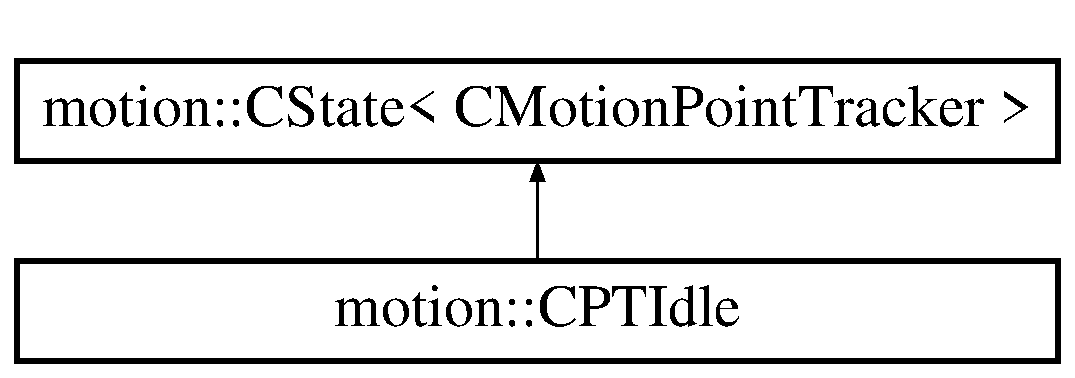
\includegraphics[height=2.000000cm]{classmotion_1_1CPTIdle}
\end{center}
\end{figure}
\subsection*{Public Member Functions}
\begin{DoxyCompactItemize}
\item 
virtual void \mbox{\hyperlink{classmotion_1_1CPTIdle_ad77ab399843dcf692d683747dbf51dd4}{enter}} (\mbox{\hyperlink{classmotion_1_1CMotionPointTracker}{C\+Motion\+Point\+Tracker}} $\ast$pt)
\item 
virtual void \mbox{\hyperlink{classmotion_1_1CPTIdle_af41acb6cf867df293faf85bfbff91940}{execute}} (\mbox{\hyperlink{classmotion_1_1CMotionPointTracker}{C\+Motion\+Point\+Tracker}} $\ast$pt)
\item 
virtual void \mbox{\hyperlink{classmotion_1_1CPTIdle_aed48db9a7d0c9364c1f93bf0787810a4}{exit}} (\mbox{\hyperlink{classmotion_1_1CMotionPointTracker}{C\+Motion\+Point\+Tracker}} $\ast$pt)
\end{DoxyCompactItemize}
\subsection*{Static Public Member Functions}
\begin{DoxyCompactItemize}
\item 
static \mbox{\hyperlink{classmotion_1_1CPTIdle}{C\+P\+T\+Idle}} $\ast$ \mbox{\hyperlink{classmotion_1_1CPTIdle_ab9b92c59fb6b828a0fd5e90ec230c1f9}{get\+Instance}} (void)
\end{DoxyCompactItemize}


\subsection{Detailed Description}
Point Tracking idle state. It will change to this state automatically when a point tracking task finished. 

\subsection{Member Function Documentation}
\mbox{\Hypertarget{classmotion_1_1CPTIdle_ad77ab399843dcf692d683747dbf51dd4}\label{classmotion_1_1CPTIdle_ad77ab399843dcf692d683747dbf51dd4}} 
\index{motion\+::\+C\+P\+T\+Idle@{motion\+::\+C\+P\+T\+Idle}!enter@{enter}}
\index{enter@{enter}!motion\+::\+C\+P\+T\+Idle@{motion\+::\+C\+P\+T\+Idle}}
\subsubsection{\texorpdfstring{enter()}{enter()}}
{\footnotesize\ttfamily void C\+P\+T\+Idle\+::enter (\begin{DoxyParamCaption}\item[{\mbox{\hyperlink{classmotion_1_1CMotionPointTracker}{C\+Motion\+Point\+Tracker}} $\ast$}]{ }\end{DoxyParamCaption})\hspace{0.3cm}{\ttfamily [virtual]}}

This will execute when the state is entered. 

Implements \mbox{\hyperlink{classmotion_1_1CState_a53d5fcfec223b58ccdd364a8430fd23c}{motion\+::\+C\+State$<$ C\+Motion\+Point\+Tracker $>$}}.

\mbox{\Hypertarget{classmotion_1_1CPTIdle_af41acb6cf867df293faf85bfbff91940}\label{classmotion_1_1CPTIdle_af41acb6cf867df293faf85bfbff91940}} 
\index{motion\+::\+C\+P\+T\+Idle@{motion\+::\+C\+P\+T\+Idle}!execute@{execute}}
\index{execute@{execute}!motion\+::\+C\+P\+T\+Idle@{motion\+::\+C\+P\+T\+Idle}}
\subsubsection{\texorpdfstring{execute()}{execute()}}
{\footnotesize\ttfamily void C\+P\+T\+Idle\+::execute (\begin{DoxyParamCaption}\item[{\mbox{\hyperlink{classmotion_1_1CMotionPointTracker}{C\+Motion\+Point\+Tracker}} $\ast$}]{ }\end{DoxyParamCaption})\hspace{0.3cm}{\ttfamily [virtual]}}

This is the states normal update function. printf(\char`\"{}\mbox{[}ljh\mbox{]} Executing Point Tracker Idle.\textbackslash{}n\char`\"{}); sleep(3); 

Implements \mbox{\hyperlink{classmotion_1_1CState_a71dc72d345b15bf3b5b5bff596a71f33}{motion\+::\+C\+State$<$ C\+Motion\+Point\+Tracker $>$}}.

\mbox{\Hypertarget{classmotion_1_1CPTIdle_aed48db9a7d0c9364c1f93bf0787810a4}\label{classmotion_1_1CPTIdle_aed48db9a7d0c9364c1f93bf0787810a4}} 
\index{motion\+::\+C\+P\+T\+Idle@{motion\+::\+C\+P\+T\+Idle}!exit@{exit}}
\index{exit@{exit}!motion\+::\+C\+P\+T\+Idle@{motion\+::\+C\+P\+T\+Idle}}
\subsubsection{\texorpdfstring{exit()}{exit()}}
{\footnotesize\ttfamily void C\+P\+T\+Idle\+::exit (\begin{DoxyParamCaption}\item[{\mbox{\hyperlink{classmotion_1_1CMotionPointTracker}{C\+Motion\+Point\+Tracker}} $\ast$}]{ }\end{DoxyParamCaption})\hspace{0.3cm}{\ttfamily [virtual]}}

This will execute when the state is exited. 

Implements \mbox{\hyperlink{classmotion_1_1CState_a353db064c159d66b82bf257b35e7c016}{motion\+::\+C\+State$<$ C\+Motion\+Point\+Tracker $>$}}.

\mbox{\Hypertarget{classmotion_1_1CPTIdle_ab9b92c59fb6b828a0fd5e90ec230c1f9}\label{classmotion_1_1CPTIdle_ab9b92c59fb6b828a0fd5e90ec230c1f9}} 
\index{motion\+::\+C\+P\+T\+Idle@{motion\+::\+C\+P\+T\+Idle}!get\+Instance@{get\+Instance}}
\index{get\+Instance@{get\+Instance}!motion\+::\+C\+P\+T\+Idle@{motion\+::\+C\+P\+T\+Idle}}
\subsubsection{\texorpdfstring{get\+Instance()}{getInstance()}}
{\footnotesize\ttfamily \mbox{\hyperlink{classmotion_1_1CPTIdle}{C\+P\+T\+Idle}} $\ast$ C\+P\+T\+Idle\+::get\+Instance (\begin{DoxyParamCaption}\item[{void}]{ }\end{DoxyParamCaption})\hspace{0.3cm}{\ttfamily [static]}}

Point Tracker initial state. 

The documentation for this class was generated from the following files\+:\begin{DoxyCompactItemize}
\item 
motion/\mbox{\hyperlink{CPTOwnedStates_8h}{C\+P\+T\+Owned\+States.\+h}}\item 
motion/\mbox{\hyperlink{CPTOwnedStates_8cpp}{C\+P\+T\+Owned\+States.\+cpp}}\end{DoxyCompactItemize}

\hypertarget{classmotion_1_1CPTTracking}{}\section{motion\+:\+:C\+P\+T\+Tracking Class Reference}
\label{classmotion_1_1CPTTracking}\index{motion\+::\+C\+P\+T\+Tracking@{motion\+::\+C\+P\+T\+Tracking}}


{\ttfamily \#include $<$C\+P\+T\+Owned\+States.\+h$>$}

Inheritance diagram for motion\+:\+:C\+P\+T\+Tracking\+:\begin{figure}[H]
\begin{center}
\leavevmode
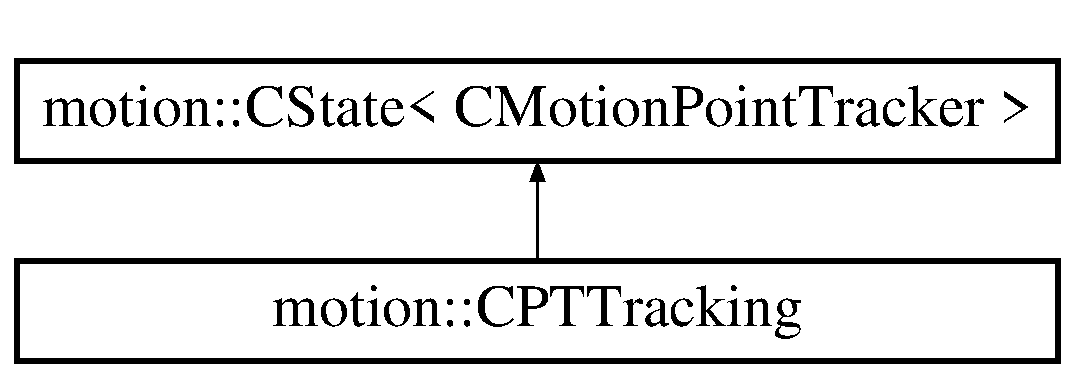
\includegraphics[height=2.000000cm]{classmotion_1_1CPTTracking}
\end{center}
\end{figure}
\subsection*{Public Member Functions}
\begin{DoxyCompactItemize}
\item 
virtual void \mbox{\hyperlink{classmotion_1_1CPTTracking_af2456aaf125ca9ba240463d1e259d4b9}{enter}} (\mbox{\hyperlink{classmotion_1_1CMotionPointTracker}{C\+Motion\+Point\+Tracker}} $\ast$pt)
\item 
virtual void \mbox{\hyperlink{classmotion_1_1CPTTracking_aa8f85da75436cc8d98c25318b0bea42d}{execute}} (\mbox{\hyperlink{classmotion_1_1CMotionPointTracker}{C\+Motion\+Point\+Tracker}} $\ast$pt)
\item 
virtual void \mbox{\hyperlink{classmotion_1_1CPTTracking_aa7a6294200e0dd2c0d53f852558d7d89}{exit}} (\mbox{\hyperlink{classmotion_1_1CMotionPointTracker}{C\+Motion\+Point\+Tracker}} $\ast$pt)
\end{DoxyCompactItemize}
\subsection*{Static Public Member Functions}
\begin{DoxyCompactItemize}
\item 
static \mbox{\hyperlink{classmotion_1_1CPTTracking}{C\+P\+T\+Tracking}} $\ast$ \mbox{\hyperlink{classmotion_1_1CPTTracking_a46a7c1bd0b68ce1c273ae32a75d76506}{get\+Instance}} (void)
\end{DoxyCompactItemize}


\subsection{Detailed Description}
Point Tracking State. 

\subsection{Member Function Documentation}
\mbox{\Hypertarget{classmotion_1_1CPTTracking_af2456aaf125ca9ba240463d1e259d4b9}\label{classmotion_1_1CPTTracking_af2456aaf125ca9ba240463d1e259d4b9}} 
\index{motion\+::\+C\+P\+T\+Tracking@{motion\+::\+C\+P\+T\+Tracking}!enter@{enter}}
\index{enter@{enter}!motion\+::\+C\+P\+T\+Tracking@{motion\+::\+C\+P\+T\+Tracking}}
\subsubsection{\texorpdfstring{enter()}{enter()}}
{\footnotesize\ttfamily void C\+P\+T\+Tracking\+::enter (\begin{DoxyParamCaption}\item[{\mbox{\hyperlink{classmotion_1_1CMotionPointTracker}{C\+Motion\+Point\+Tracker}} $\ast$}]{ }\end{DoxyParamCaption})\hspace{0.3cm}{\ttfamily [virtual]}}

This will execute when the state is entered. 

Implements \mbox{\hyperlink{classmotion_1_1CState_a53d5fcfec223b58ccdd364a8430fd23c}{motion\+::\+C\+State$<$ C\+Motion\+Point\+Tracker $>$}}.

\mbox{\Hypertarget{classmotion_1_1CPTTracking_aa8f85da75436cc8d98c25318b0bea42d}\label{classmotion_1_1CPTTracking_aa8f85da75436cc8d98c25318b0bea42d}} 
\index{motion\+::\+C\+P\+T\+Tracking@{motion\+::\+C\+P\+T\+Tracking}!execute@{execute}}
\index{execute@{execute}!motion\+::\+C\+P\+T\+Tracking@{motion\+::\+C\+P\+T\+Tracking}}
\subsubsection{\texorpdfstring{execute()}{execute()}}
{\footnotesize\ttfamily void C\+P\+T\+Tracking\+::execute (\begin{DoxyParamCaption}\item[{\mbox{\hyperlink{classmotion_1_1CMotionPointTracker}{C\+Motion\+Point\+Tracker}} $\ast$}]{ }\end{DoxyParamCaption})\hspace{0.3cm}{\ttfamily [virtual]}}

This is the states normal update function. todos\+: obs check, etc. 

Implements \mbox{\hyperlink{classmotion_1_1CState_a71dc72d345b15bf3b5b5bff596a71f33}{motion\+::\+C\+State$<$ C\+Motion\+Point\+Tracker $>$}}.

\mbox{\Hypertarget{classmotion_1_1CPTTracking_aa7a6294200e0dd2c0d53f852558d7d89}\label{classmotion_1_1CPTTracking_aa7a6294200e0dd2c0d53f852558d7d89}} 
\index{motion\+::\+C\+P\+T\+Tracking@{motion\+::\+C\+P\+T\+Tracking}!exit@{exit}}
\index{exit@{exit}!motion\+::\+C\+P\+T\+Tracking@{motion\+::\+C\+P\+T\+Tracking}}
\subsubsection{\texorpdfstring{exit()}{exit()}}
{\footnotesize\ttfamily void C\+P\+T\+Tracking\+::exit (\begin{DoxyParamCaption}\item[{\mbox{\hyperlink{classmotion_1_1CMotionPointTracker}{C\+Motion\+Point\+Tracker}} $\ast$}]{ }\end{DoxyParamCaption})\hspace{0.3cm}{\ttfamily [virtual]}}

This will execute when the state is exited. todo 

Implements \mbox{\hyperlink{classmotion_1_1CState_a353db064c159d66b82bf257b35e7c016}{motion\+::\+C\+State$<$ C\+Motion\+Point\+Tracker $>$}}.

\mbox{\Hypertarget{classmotion_1_1CPTTracking_a46a7c1bd0b68ce1c273ae32a75d76506}\label{classmotion_1_1CPTTracking_a46a7c1bd0b68ce1c273ae32a75d76506}} 
\index{motion\+::\+C\+P\+T\+Tracking@{motion\+::\+C\+P\+T\+Tracking}!get\+Instance@{get\+Instance}}
\index{get\+Instance@{get\+Instance}!motion\+::\+C\+P\+T\+Tracking@{motion\+::\+C\+P\+T\+Tracking}}
\subsubsection{\texorpdfstring{get\+Instance()}{getInstance()}}
{\footnotesize\ttfamily \mbox{\hyperlink{classmotion_1_1CPTTracking}{C\+P\+T\+Tracking}} $\ast$ C\+P\+T\+Tracking\+::get\+Instance (\begin{DoxyParamCaption}\item[{void}]{ }\end{DoxyParamCaption})\hspace{0.3cm}{\ttfamily [static]}}

Point Tracker Methods. 

The documentation for this class was generated from the following files\+:\begin{DoxyCompactItemize}
\item 
motion/\mbox{\hyperlink{CPTOwnedStates_8h}{C\+P\+T\+Owned\+States.\+h}}\item 
motion/\mbox{\hyperlink{CPTOwnedStates_8cpp}{C\+P\+T\+Owned\+States.\+cpp}}\end{DoxyCompactItemize}

\hypertarget{classmotion_1_1CState}{}\section{motion\+:\+:C\+State$<$ state\+\_\+type $>$ Class Template Reference}
\label{classmotion_1_1CState}\index{motion\+::\+C\+State$<$ state\+\_\+type $>$@{motion\+::\+C\+State$<$ state\+\_\+type $>$}}
\subsection*{Public Member Functions}
\begin{DoxyCompactItemize}
\item 
virtual void \mbox{\hyperlink{classmotion_1_1CState_a53d5fcfec223b58ccdd364a8430fd23c}{enter}} (state\+\_\+type $\ast$)=0
\item 
virtual void \mbox{\hyperlink{classmotion_1_1CState_a71dc72d345b15bf3b5b5bff596a71f33}{execute}} (state\+\_\+type $\ast$)=0
\item 
virtual void \mbox{\hyperlink{classmotion_1_1CState_a353db064c159d66b82bf257b35e7c016}{exit}} (state\+\_\+type $\ast$)=0
\end{DoxyCompactItemize}


\subsection{Member Function Documentation}
\mbox{\Hypertarget{classmotion_1_1CState_a53d5fcfec223b58ccdd364a8430fd23c}\label{classmotion_1_1CState_a53d5fcfec223b58ccdd364a8430fd23c}} 
\index{motion\+::\+C\+State@{motion\+::\+C\+State}!enter@{enter}}
\index{enter@{enter}!motion\+::\+C\+State@{motion\+::\+C\+State}}
\subsubsection{\texorpdfstring{enter()}{enter()}}
{\footnotesize\ttfamily template$<$class state\+\_\+type$>$ \\
virtual void \mbox{\hyperlink{classmotion_1_1CState}{motion\+::\+C\+State}}$<$ state\+\_\+type $>$\+::enter (\begin{DoxyParamCaption}\item[{state\+\_\+type $\ast$}]{ }\end{DoxyParamCaption})\hspace{0.3cm}{\ttfamily [pure virtual]}}

This will execute when the state is entered. \mbox{\Hypertarget{classmotion_1_1CState_a71dc72d345b15bf3b5b5bff596a71f33}\label{classmotion_1_1CState_a71dc72d345b15bf3b5b5bff596a71f33}} 
\index{motion\+::\+C\+State@{motion\+::\+C\+State}!execute@{execute}}
\index{execute@{execute}!motion\+::\+C\+State@{motion\+::\+C\+State}}
\subsubsection{\texorpdfstring{execute()}{execute()}}
{\footnotesize\ttfamily template$<$class state\+\_\+type$>$ \\
virtual void \mbox{\hyperlink{classmotion_1_1CState}{motion\+::\+C\+State}}$<$ state\+\_\+type $>$\+::execute (\begin{DoxyParamCaption}\item[{state\+\_\+type $\ast$}]{ }\end{DoxyParamCaption})\hspace{0.3cm}{\ttfamily [pure virtual]}}

This is the states normal update function. \mbox{\Hypertarget{classmotion_1_1CState_a353db064c159d66b82bf257b35e7c016}\label{classmotion_1_1CState_a353db064c159d66b82bf257b35e7c016}} 
\index{motion\+::\+C\+State@{motion\+::\+C\+State}!exit@{exit}}
\index{exit@{exit}!motion\+::\+C\+State@{motion\+::\+C\+State}}
\subsubsection{\texorpdfstring{exit()}{exit()}}
{\footnotesize\ttfamily template$<$class state\+\_\+type$>$ \\
virtual void \mbox{\hyperlink{classmotion_1_1CState}{motion\+::\+C\+State}}$<$ state\+\_\+type $>$\+::exit (\begin{DoxyParamCaption}\item[{state\+\_\+type $\ast$}]{ }\end{DoxyParamCaption})\hspace{0.3cm}{\ttfamily [pure virtual]}}

This will execute when the state is exited. 

The documentation for this class was generated from the following file\+:\begin{DoxyCompactItemize}
\item 
motion/C\+State.\+h\end{DoxyCompactItemize}

\hypertarget{classmotion_1_1CStateMachine}{}\section{motion\+:\+:C\+State\+Machine$<$ state\+\_\+type $>$ Class Template Reference}
\label{classmotion_1_1CStateMachine}\index{motion\+::\+C\+State\+Machine$<$ state\+\_\+type $>$@{motion\+::\+C\+State\+Machine$<$ state\+\_\+type $>$}}
\subsection*{Public Member Functions}
\begin{DoxyCompactItemize}
\item 
\mbox{\Hypertarget{classmotion_1_1CStateMachine_ac91f606bd5d004771294c02a3990f7ed}\label{classmotion_1_1CStateMachine_ac91f606bd5d004771294c02a3990f7ed}} 
{\bfseries C\+State\+Machine} (state\+\_\+type $\ast$owner)
\item 
void \mbox{\hyperlink{classmotion_1_1CStateMachine_a57407660e1054b7b6e912efc3afb9495}{set\+Current\+State}} (\mbox{\hyperlink{classmotion_1_1CState}{C\+State}}$<$ state\+\_\+type $>$ $\ast$s)
\item 
\mbox{\Hypertarget{classmotion_1_1CStateMachine_aaeead01662f75ed768226163665bcec4}\label{classmotion_1_1CStateMachine_aaeead01662f75ed768226163665bcec4}} 
void {\bfseries set\+Global\+State} (\mbox{\hyperlink{classmotion_1_1CState}{C\+State}}$<$ state\+\_\+type $>$ $\ast$s)
\item 
\mbox{\Hypertarget{classmotion_1_1CStateMachine_a55764d2e385cb61f26e6aa09f80577e4}\label{classmotion_1_1CStateMachine_a55764d2e385cb61f26e6aa09f80577e4}} 
void {\bfseries set\+Previous\+State} (\mbox{\hyperlink{classmotion_1_1CState}{C\+State}}$<$ state\+\_\+type $>$ $\ast$s)
\item 
void \mbox{\hyperlink{classmotion_1_1CStateMachine_a8a944b6b5dcff9b614b434fabcd8955c}{update}} () const
\item 
void \mbox{\hyperlink{classmotion_1_1CStateMachine_a13d97b778f850709c7f9060de4aba142}{change\+State}} (\mbox{\hyperlink{classmotion_1_1CState}{C\+State}}$<$ state\+\_\+type $>$ $\ast$p\+New\+State)
\item 
void \mbox{\hyperlink{classmotion_1_1CStateMachine_ae8e1d802793aded65b1da25dad007486}{revert\+To\+Previous\+State}} ()
\item 
\mbox{\hyperlink{classmotion_1_1CState}{C\+State}}$<$ state\+\_\+type $>$ $\ast$ \mbox{\hyperlink{classmotion_1_1CStateMachine_a2231e1232b1fe6a793b95e0e2217f362}{get\+Current\+State}} (void) const
\item 
\mbox{\Hypertarget{classmotion_1_1CStateMachine_ac9e635be4cb960479c6cdef54966480b}\label{classmotion_1_1CStateMachine_ac9e635be4cb960479c6cdef54966480b}} 
\mbox{\hyperlink{classmotion_1_1CState}{C\+State}}$<$ state\+\_\+type $>$ $\ast$ {\bfseries get\+Global\+State} (void) const
\item 
\mbox{\Hypertarget{classmotion_1_1CStateMachine_acab2aefef8b1fa57d211eb68aa8e96f8}\label{classmotion_1_1CStateMachine_acab2aefef8b1fa57d211eb68aa8e96f8}} 
\mbox{\hyperlink{classmotion_1_1CState}{C\+State}}$<$ state\+\_\+type $>$ $\ast$ {\bfseries get\+Previous\+State} (void) const
\end{DoxyCompactItemize}


\subsection{Member Function Documentation}
\mbox{\Hypertarget{classmotion_1_1CStateMachine_a13d97b778f850709c7f9060de4aba142}\label{classmotion_1_1CStateMachine_a13d97b778f850709c7f9060de4aba142}} 
\index{motion\+::\+C\+State\+Machine@{motion\+::\+C\+State\+Machine}!change\+State@{change\+State}}
\index{change\+State@{change\+State}!motion\+::\+C\+State\+Machine@{motion\+::\+C\+State\+Machine}}
\subsubsection{\texorpdfstring{change\+State()}{changeState()}}
{\footnotesize\ttfamily template$<$class state\+\_\+type$>$ \\
void \mbox{\hyperlink{classmotion_1_1CStateMachine}{motion\+::\+C\+State\+Machine}}$<$ state\+\_\+type $>$\+::change\+State (\begin{DoxyParamCaption}\item[{\mbox{\hyperlink{classmotion_1_1CState}{C\+State}}$<$ state\+\_\+type $>$ $\ast$}]{p\+New\+State }\end{DoxyParamCaption})\hspace{0.3cm}{\ttfamily [inline]}}

Change to a new state. Keep a record of the previous state. ~\newline
~\newline
~\newline
 Call the exit method of the existing state. ~\newline
~\newline
 Change state to the new state. ~\newline
 Call the entry method of the new state. \mbox{\Hypertarget{classmotion_1_1CStateMachine_a2231e1232b1fe6a793b95e0e2217f362}\label{classmotion_1_1CStateMachine_a2231e1232b1fe6a793b95e0e2217f362}} 
\index{motion\+::\+C\+State\+Machine@{motion\+::\+C\+State\+Machine}!get\+Current\+State@{get\+Current\+State}}
\index{get\+Current\+State@{get\+Current\+State}!motion\+::\+C\+State\+Machine@{motion\+::\+C\+State\+Machine}}
\subsubsection{\texorpdfstring{get\+Current\+State()}{getCurrentState()}}
{\footnotesize\ttfamily template$<$class state\+\_\+type$>$ \\
\mbox{\hyperlink{classmotion_1_1CState}{C\+State}}$<$state\+\_\+type$>$$\ast$ \mbox{\hyperlink{classmotion_1_1CStateMachine}{motion\+::\+C\+State\+Machine}}$<$ state\+\_\+type $>$\+::get\+Current\+State (\begin{DoxyParamCaption}\item[{void}]{ }\end{DoxyParamCaption}) const\hspace{0.3cm}{\ttfamily [inline]}}

Returns true if the current state\textquotesingle{}s type is equal to the type of the class passed as a parameter.\+bool is\+In\+State(const C\+State$<$state\+\_\+type$>$\& st) const \{ return typeid($\ast$m\+\_\+p\+Current\+State) == typeid(st); \} \mbox{\Hypertarget{classmotion_1_1CStateMachine_ae8e1d802793aded65b1da25dad007486}\label{classmotion_1_1CStateMachine_ae8e1d802793aded65b1da25dad007486}} 
\index{motion\+::\+C\+State\+Machine@{motion\+::\+C\+State\+Machine}!revert\+To\+Previous\+State@{revert\+To\+Previous\+State}}
\index{revert\+To\+Previous\+State@{revert\+To\+Previous\+State}!motion\+::\+C\+State\+Machine@{motion\+::\+C\+State\+Machine}}
\subsubsection{\texorpdfstring{revert\+To\+Previous\+State()}{revertToPreviousState()}}
{\footnotesize\ttfamily template$<$class state\+\_\+type$>$ \\
void \mbox{\hyperlink{classmotion_1_1CStateMachine}{motion\+::\+C\+State\+Machine}}$<$ state\+\_\+type $>$\+::revert\+To\+Previous\+State (\begin{DoxyParamCaption}{ }\end{DoxyParamCaption})\hspace{0.3cm}{\ttfamily [inline]}}

Change state back to the previous state. \mbox{\Hypertarget{classmotion_1_1CStateMachine_a57407660e1054b7b6e912efc3afb9495}\label{classmotion_1_1CStateMachine_a57407660e1054b7b6e912efc3afb9495}} 
\index{motion\+::\+C\+State\+Machine@{motion\+::\+C\+State\+Machine}!set\+Current\+State@{set\+Current\+State}}
\index{set\+Current\+State@{set\+Current\+State}!motion\+::\+C\+State\+Machine@{motion\+::\+C\+State\+Machine}}
\subsubsection{\texorpdfstring{set\+Current\+State()}{setCurrentState()}}
{\footnotesize\ttfamily template$<$class state\+\_\+type$>$ \\
void \mbox{\hyperlink{classmotion_1_1CStateMachine}{motion\+::\+C\+State\+Machine}}$<$ state\+\_\+type $>$\+::set\+Current\+State (\begin{DoxyParamCaption}\item[{\mbox{\hyperlink{classmotion_1_1CState}{C\+State}}$<$ state\+\_\+type $>$ $\ast$}]{s }\end{DoxyParamCaption})\hspace{0.3cm}{\ttfamily [inline]}}

Use these methods to initialize the F\+SM. \mbox{\Hypertarget{classmotion_1_1CStateMachine_a8a944b6b5dcff9b614b434fabcd8955c}\label{classmotion_1_1CStateMachine_a8a944b6b5dcff9b614b434fabcd8955c}} 
\index{motion\+::\+C\+State\+Machine@{motion\+::\+C\+State\+Machine}!update@{update}}
\index{update@{update}!motion\+::\+C\+State\+Machine@{motion\+::\+C\+State\+Machine}}
\subsubsection{\texorpdfstring{update()}{update()}}
{\footnotesize\ttfamily template$<$class state\+\_\+type$>$ \\
void \mbox{\hyperlink{classmotion_1_1CStateMachine}{motion\+::\+C\+State\+Machine}}$<$ state\+\_\+type $>$\+::update (\begin{DoxyParamCaption}\item[{void}]{ }\end{DoxyParamCaption}) const\hspace{0.3cm}{\ttfamily [inline]}}

Call this to update the F\+SM. If a global state exists, call its execute method, else do nothing. ~\newline
~\newline
 if(m\+\_\+p\+Global\+State) m\+\_\+p\+Global\+State-\/$>$execute(m\+\_\+p\+Owner);

Same for the current state. 

The documentation for this class was generated from the following file\+:\begin{DoxyCompactItemize}
\item 
motion/\mbox{\hyperlink{CStateMachine_8h}{C\+State\+Machine.\+h}}\end{DoxyCompactItemize}

\hypertarget{classmotion_1_1CWFObsAvoid}{}\section{motion\+:\+:C\+W\+F\+Obs\+Avoid Class Reference}
\label{classmotion_1_1CWFObsAvoid}\index{motion\+::\+C\+W\+F\+Obs\+Avoid@{motion\+::\+C\+W\+F\+Obs\+Avoid}}


{\ttfamily \#include $<$C\+W\+F\+Owned\+States.\+h$>$}

Inheritance diagram for motion\+:\+:C\+W\+F\+Obs\+Avoid\+:\begin{figure}[H]
\begin{center}
\leavevmode
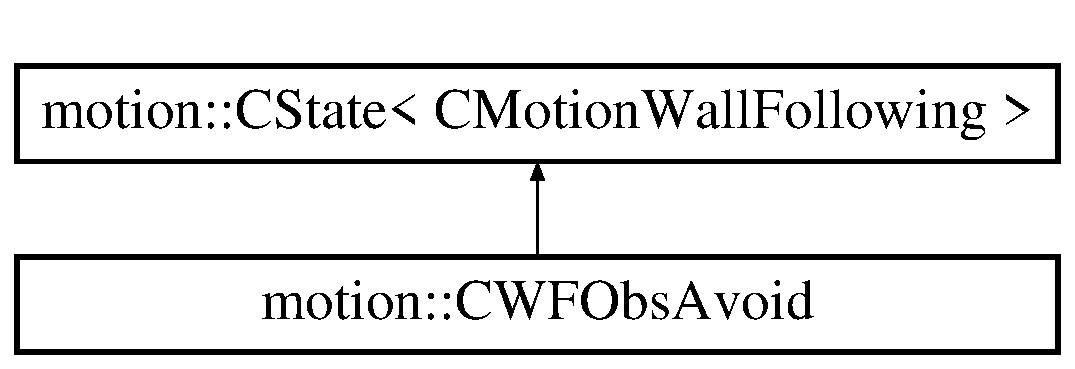
\includegraphics[height=2.000000cm]{classmotion_1_1CWFObsAvoid}
\end{center}
\end{figure}
\subsection*{Public Member Functions}
\begin{DoxyCompactItemize}
\item 
virtual void \mbox{\hyperlink{classmotion_1_1CWFObsAvoid_aee2e80e821ecd29528f048c99813b63a}{enter}} (\mbox{\hyperlink{classmotion_1_1CMotionWallFollowing}{C\+Motion\+Wall\+Following}} $\ast$wf)
\item 
virtual void \mbox{\hyperlink{classmotion_1_1CWFObsAvoid_a458771fccc326a8b02e4f947cdbb7f3b}{execute}} (\mbox{\hyperlink{classmotion_1_1CMotionWallFollowing}{C\+Motion\+Wall\+Following}} $\ast$wf)
\item 
virtual void \mbox{\hyperlink{classmotion_1_1CWFObsAvoid_af95e36cbc64c2c47fdf5d6ad5dde90a8}{exit}} (\mbox{\hyperlink{classmotion_1_1CMotionWallFollowing}{C\+Motion\+Wall\+Following}} $\ast$wf)
\end{DoxyCompactItemize}
\subsection*{Static Public Member Functions}
\begin{DoxyCompactItemize}
\item 
static \mbox{\hyperlink{classmotion_1_1CWFObsAvoid}{C\+W\+F\+Obs\+Avoid}} $\ast$ \mbox{\hyperlink{classmotion_1_1CWFObsAvoid_a67a97a1719b8d637a9cf154bd8977171}{get\+Instance}} (void)
\end{DoxyCompactItemize}


\subsection{Detailed Description}
Obstacle Avoidance State. When the ahead distance is small enough, sub-\/motion will change to this state. 

\subsection{Member Function Documentation}
\mbox{\Hypertarget{classmotion_1_1CWFObsAvoid_aee2e80e821ecd29528f048c99813b63a}\label{classmotion_1_1CWFObsAvoid_aee2e80e821ecd29528f048c99813b63a}} 
\index{motion\+::\+C\+W\+F\+Obs\+Avoid@{motion\+::\+C\+W\+F\+Obs\+Avoid}!enter@{enter}}
\index{enter@{enter}!motion\+::\+C\+W\+F\+Obs\+Avoid@{motion\+::\+C\+W\+F\+Obs\+Avoid}}
\subsubsection{\texorpdfstring{enter()}{enter()}}
{\footnotesize\ttfamily void C\+W\+F\+Obs\+Avoid\+::enter (\begin{DoxyParamCaption}\item[{\mbox{\hyperlink{classmotion_1_1CMotionWallFollowing}{C\+Motion\+Wall\+Following}} $\ast$}]{ }\end{DoxyParamCaption})\hspace{0.3cm}{\ttfamily [virtual]}}

This will execute when the state is entered. 

Implements \mbox{\hyperlink{classmotion_1_1CState_a53d5fcfec223b58ccdd364a8430fd23c}{motion\+::\+C\+State$<$ C\+Motion\+Wall\+Following $>$}}.

\mbox{\Hypertarget{classmotion_1_1CWFObsAvoid_a458771fccc326a8b02e4f947cdbb7f3b}\label{classmotion_1_1CWFObsAvoid_a458771fccc326a8b02e4f947cdbb7f3b}} 
\index{motion\+::\+C\+W\+F\+Obs\+Avoid@{motion\+::\+C\+W\+F\+Obs\+Avoid}!execute@{execute}}
\index{execute@{execute}!motion\+::\+C\+W\+F\+Obs\+Avoid@{motion\+::\+C\+W\+F\+Obs\+Avoid}}
\subsubsection{\texorpdfstring{execute()}{execute()}}
{\footnotesize\ttfamily void C\+W\+F\+Obs\+Avoid\+::execute (\begin{DoxyParamCaption}\item[{\mbox{\hyperlink{classmotion_1_1CMotionWallFollowing}{C\+Motion\+Wall\+Following}} $\ast$}]{ }\end{DoxyParamCaption})\hspace{0.3cm}{\ttfamily [virtual]}}

This is the states normal update function. todo 

Implements \mbox{\hyperlink{classmotion_1_1CState_a71dc72d345b15bf3b5b5bff596a71f33}{motion\+::\+C\+State$<$ C\+Motion\+Wall\+Following $>$}}.

\mbox{\Hypertarget{classmotion_1_1CWFObsAvoid_af95e36cbc64c2c47fdf5d6ad5dde90a8}\label{classmotion_1_1CWFObsAvoid_af95e36cbc64c2c47fdf5d6ad5dde90a8}} 
\index{motion\+::\+C\+W\+F\+Obs\+Avoid@{motion\+::\+C\+W\+F\+Obs\+Avoid}!exit@{exit}}
\index{exit@{exit}!motion\+::\+C\+W\+F\+Obs\+Avoid@{motion\+::\+C\+W\+F\+Obs\+Avoid}}
\subsubsection{\texorpdfstring{exit()}{exit()}}
{\footnotesize\ttfamily void C\+W\+F\+Obs\+Avoid\+::exit (\begin{DoxyParamCaption}\item[{\mbox{\hyperlink{classmotion_1_1CMotionWallFollowing}{C\+Motion\+Wall\+Following}} $\ast$}]{ }\end{DoxyParamCaption})\hspace{0.3cm}{\ttfamily [virtual]}}

This will execute when the state is exited. 

Implements \mbox{\hyperlink{classmotion_1_1CState_a353db064c159d66b82bf257b35e7c016}{motion\+::\+C\+State$<$ C\+Motion\+Wall\+Following $>$}}.

\mbox{\Hypertarget{classmotion_1_1CWFObsAvoid_a67a97a1719b8d637a9cf154bd8977171}\label{classmotion_1_1CWFObsAvoid_a67a97a1719b8d637a9cf154bd8977171}} 
\index{motion\+::\+C\+W\+F\+Obs\+Avoid@{motion\+::\+C\+W\+F\+Obs\+Avoid}!get\+Instance@{get\+Instance}}
\index{get\+Instance@{get\+Instance}!motion\+::\+C\+W\+F\+Obs\+Avoid@{motion\+::\+C\+W\+F\+Obs\+Avoid}}
\subsubsection{\texorpdfstring{get\+Instance()}{getInstance()}}
{\footnotesize\ttfamily \mbox{\hyperlink{classmotion_1_1CWFObsAvoid}{C\+W\+F\+Obs\+Avoid}} $\ast$ C\+W\+F\+Obs\+Avoid\+::get\+Instance (\begin{DoxyParamCaption}\item[{void}]{ }\end{DoxyParamCaption})\hspace{0.3cm}{\ttfamily [static]}}

Obstacle Avoidance Methods. 

The documentation for this class was generated from the following files\+:\begin{DoxyCompactItemize}
\item 
motion/\mbox{\hyperlink{CWFOwnedStates_8h}{C\+W\+F\+Owned\+States.\+h}}\item 
motion/\mbox{\hyperlink{CWFOwnedStates_8cpp}{C\+W\+F\+Owned\+States.\+cpp}}\end{DoxyCompactItemize}

\hypertarget{classmotion_1_1CWFRidgeTrack}{}\section{motion\+:\+:C\+W\+F\+Ridge\+Track Class Reference}
\label{classmotion_1_1CWFRidgeTrack}\index{motion\+::\+C\+W\+F\+Ridge\+Track@{motion\+::\+C\+W\+F\+Ridge\+Track}}


{\ttfamily \#include $<$C\+W\+F\+Owned\+States.\+h$>$}

Inheritance diagram for motion\+:\+:C\+W\+F\+Ridge\+Track\+:\begin{figure}[H]
\begin{center}
\leavevmode
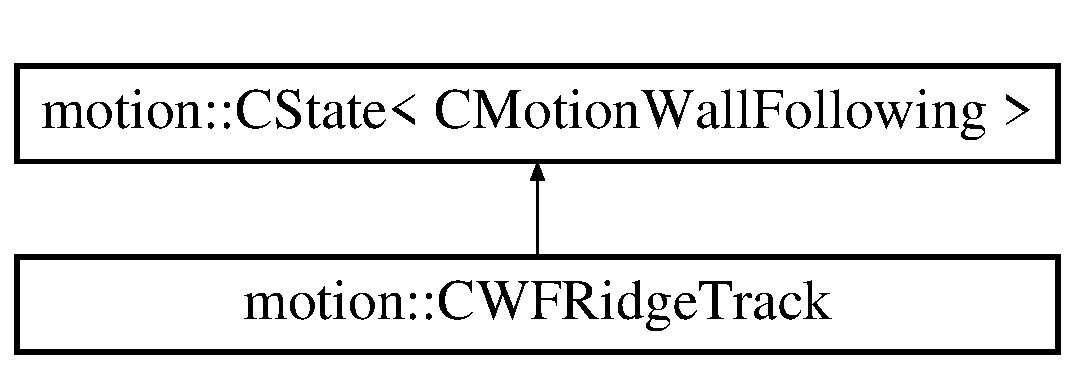
\includegraphics[height=2.000000cm]{classmotion_1_1CWFRidgeTrack}
\end{center}
\end{figure}
\subsection*{Public Member Functions}
\begin{DoxyCompactItemize}
\item 
virtual void \mbox{\hyperlink{classmotion_1_1CWFRidgeTrack_a216b8b7778464a2afd1a4f57da4317de}{enter}} (\mbox{\hyperlink{classmotion_1_1CMotionWallFollowing}{C\+Motion\+Wall\+Following}} $\ast$wf)
\item 
virtual void \mbox{\hyperlink{classmotion_1_1CWFRidgeTrack_a68b351694d461637ad97c5d657f3fbca}{execute}} (\mbox{\hyperlink{classmotion_1_1CMotionWallFollowing}{C\+Motion\+Wall\+Following}} $\ast$wf)
\item 
virtual void \mbox{\hyperlink{classmotion_1_1CWFRidgeTrack_a15ab958b412e2e6a70619822e6697f7f}{exit}} (\mbox{\hyperlink{classmotion_1_1CMotionWallFollowing}{C\+Motion\+Wall\+Following}} $\ast$wf)
\end{DoxyCompactItemize}
\subsection*{Static Public Member Functions}
\begin{DoxyCompactItemize}
\item 
static \mbox{\hyperlink{classmotion_1_1CWFRidgeTrack}{C\+W\+F\+Ridge\+Track}} $\ast$ \mbox{\hyperlink{classmotion_1_1CWFRidgeTrack_ad85de711d4ce2b59f3dca20d233d77ed}{get\+Instance}} (void)
\end{DoxyCompactItemize}


\subsection{Detailed Description}
Ridge Tracking State. When the side distance have big jump, sub-\/motion will change to this state. 

\subsection{Member Function Documentation}
\mbox{\Hypertarget{classmotion_1_1CWFRidgeTrack_a216b8b7778464a2afd1a4f57da4317de}\label{classmotion_1_1CWFRidgeTrack_a216b8b7778464a2afd1a4f57da4317de}} 
\index{motion\+::\+C\+W\+F\+Ridge\+Track@{motion\+::\+C\+W\+F\+Ridge\+Track}!enter@{enter}}
\index{enter@{enter}!motion\+::\+C\+W\+F\+Ridge\+Track@{motion\+::\+C\+W\+F\+Ridge\+Track}}
\subsubsection{\texorpdfstring{enter()}{enter()}}
{\footnotesize\ttfamily void C\+W\+F\+Ridge\+Track\+::enter (\begin{DoxyParamCaption}\item[{\mbox{\hyperlink{classmotion_1_1CMotionWallFollowing}{C\+Motion\+Wall\+Following}} $\ast$}]{ }\end{DoxyParamCaption})\hspace{0.3cm}{\ttfamily [virtual]}}

This will execute when the state is entered. 

Implements \mbox{\hyperlink{classmotion_1_1CState_a53d5fcfec223b58ccdd364a8430fd23c}{motion\+::\+C\+State$<$ C\+Motion\+Wall\+Following $>$}}.

\mbox{\Hypertarget{classmotion_1_1CWFRidgeTrack_a68b351694d461637ad97c5d657f3fbca}\label{classmotion_1_1CWFRidgeTrack_a68b351694d461637ad97c5d657f3fbca}} 
\index{motion\+::\+C\+W\+F\+Ridge\+Track@{motion\+::\+C\+W\+F\+Ridge\+Track}!execute@{execute}}
\index{execute@{execute}!motion\+::\+C\+W\+F\+Ridge\+Track@{motion\+::\+C\+W\+F\+Ridge\+Track}}
\subsubsection{\texorpdfstring{execute()}{execute()}}
{\footnotesize\ttfamily void C\+W\+F\+Ridge\+Track\+::execute (\begin{DoxyParamCaption}\item[{\mbox{\hyperlink{classmotion_1_1CMotionWallFollowing}{C\+Motion\+Wall\+Following}} $\ast$}]{ }\end{DoxyParamCaption})\hspace{0.3cm}{\ttfamily [virtual]}}

This is the states normal update function. todo 

Implements \mbox{\hyperlink{classmotion_1_1CState_a71dc72d345b15bf3b5b5bff596a71f33}{motion\+::\+C\+State$<$ C\+Motion\+Wall\+Following $>$}}.

\mbox{\Hypertarget{classmotion_1_1CWFRidgeTrack_a15ab958b412e2e6a70619822e6697f7f}\label{classmotion_1_1CWFRidgeTrack_a15ab958b412e2e6a70619822e6697f7f}} 
\index{motion\+::\+C\+W\+F\+Ridge\+Track@{motion\+::\+C\+W\+F\+Ridge\+Track}!exit@{exit}}
\index{exit@{exit}!motion\+::\+C\+W\+F\+Ridge\+Track@{motion\+::\+C\+W\+F\+Ridge\+Track}}
\subsubsection{\texorpdfstring{exit()}{exit()}}
{\footnotesize\ttfamily void C\+W\+F\+Ridge\+Track\+::exit (\begin{DoxyParamCaption}\item[{\mbox{\hyperlink{classmotion_1_1CMotionWallFollowing}{C\+Motion\+Wall\+Following}} $\ast$}]{ }\end{DoxyParamCaption})\hspace{0.3cm}{\ttfamily [virtual]}}

This will execute when the state is exited. 

Implements \mbox{\hyperlink{classmotion_1_1CState_a353db064c159d66b82bf257b35e7c016}{motion\+::\+C\+State$<$ C\+Motion\+Wall\+Following $>$}}.

\mbox{\Hypertarget{classmotion_1_1CWFRidgeTrack_ad85de711d4ce2b59f3dca20d233d77ed}\label{classmotion_1_1CWFRidgeTrack_ad85de711d4ce2b59f3dca20d233d77ed}} 
\index{motion\+::\+C\+W\+F\+Ridge\+Track@{motion\+::\+C\+W\+F\+Ridge\+Track}!get\+Instance@{get\+Instance}}
\index{get\+Instance@{get\+Instance}!motion\+::\+C\+W\+F\+Ridge\+Track@{motion\+::\+C\+W\+F\+Ridge\+Track}}
\subsubsection{\texorpdfstring{get\+Instance()}{getInstance()}}
{\footnotesize\ttfamily \mbox{\hyperlink{classmotion_1_1CWFRidgeTrack}{C\+W\+F\+Ridge\+Track}} $\ast$ C\+W\+F\+Ridge\+Track\+::get\+Instance (\begin{DoxyParamCaption}\item[{void}]{ }\end{DoxyParamCaption})\hspace{0.3cm}{\ttfamily [static]}}

Ridge Tracking Methods. 

The documentation for this class was generated from the following files\+:\begin{DoxyCompactItemize}
\item 
motion/\mbox{\hyperlink{CWFOwnedStates_8h}{C\+W\+F\+Owned\+States.\+h}}\item 
motion/\mbox{\hyperlink{CWFOwnedStates_8cpp}{C\+W\+F\+Owned\+States.\+cpp}}\end{DoxyCompactItemize}

\hypertarget{classmotion_1_1CWFWallFol}{}\section{motion\+:\+:C\+W\+F\+Wall\+Fol Class Reference}
\label{classmotion_1_1CWFWallFol}\index{motion\+::\+C\+W\+F\+Wall\+Fol@{motion\+::\+C\+W\+F\+Wall\+Fol}}


{\ttfamily \#include $<$C\+W\+F\+Owned\+States.\+h$>$}

Inheritance diagram for motion\+:\+:C\+W\+F\+Wall\+Fol\+:\begin{figure}[H]
\begin{center}
\leavevmode
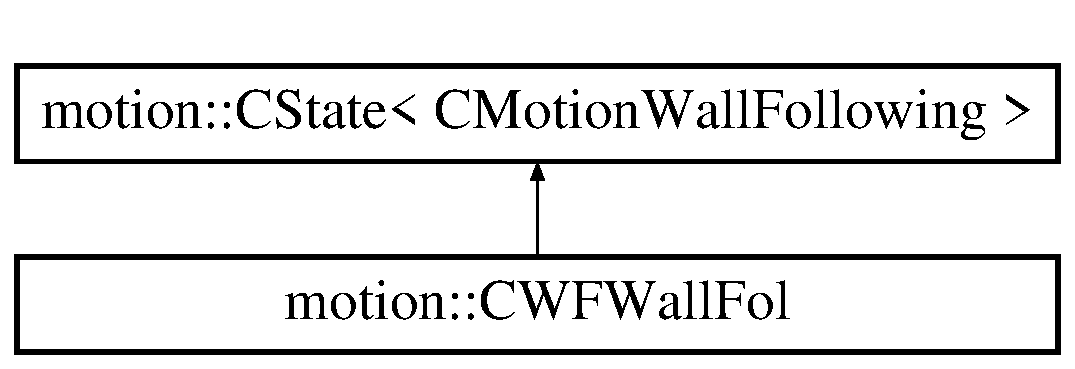
\includegraphics[height=2.000000cm]{classmotion_1_1CWFWallFol}
\end{center}
\end{figure}
\subsection*{Public Member Functions}
\begin{DoxyCompactItemize}
\item 
virtual void \mbox{\hyperlink{classmotion_1_1CWFWallFol_a4d0e6d05a5bc89c690f86559cbc55ecb}{enter}} (\mbox{\hyperlink{classmotion_1_1CMotionWallFollowing}{C\+Motion\+Wall\+Following}} $\ast$wf)
\item 
virtual void \mbox{\hyperlink{classmotion_1_1CWFWallFol_a089095864c2340123e6e5e5e4e08ef23}{execute}} (\mbox{\hyperlink{classmotion_1_1CMotionWallFollowing}{C\+Motion\+Wall\+Following}} $\ast$wf)
\item 
virtual void \mbox{\hyperlink{classmotion_1_1CWFWallFol_af90587d832a04a15d6c166e9b6a6afed}{exit}} (\mbox{\hyperlink{classmotion_1_1CMotionWallFollowing}{C\+Motion\+Wall\+Following}} $\ast$wf)
\end{DoxyCompactItemize}
\subsection*{Static Public Member Functions}
\begin{DoxyCompactItemize}
\item 
static \mbox{\hyperlink{classmotion_1_1CWFWallFol}{C\+W\+F\+Wall\+Fol}} $\ast$ \mbox{\hyperlink{classmotion_1_1CWFWallFol_a56dd0cbd1e50c6e845a9c944e0b9a0a9}{get\+Instance}} (void)
\end{DoxyCompactItemize}


\subsection{Detailed Description}
Wall Following State. 

\subsection{Member Function Documentation}
\mbox{\Hypertarget{classmotion_1_1CWFWallFol_a4d0e6d05a5bc89c690f86559cbc55ecb}\label{classmotion_1_1CWFWallFol_a4d0e6d05a5bc89c690f86559cbc55ecb}} 
\index{motion\+::\+C\+W\+F\+Wall\+Fol@{motion\+::\+C\+W\+F\+Wall\+Fol}!enter@{enter}}
\index{enter@{enter}!motion\+::\+C\+W\+F\+Wall\+Fol@{motion\+::\+C\+W\+F\+Wall\+Fol}}
\subsubsection{\texorpdfstring{enter()}{enter()}}
{\footnotesize\ttfamily void C\+W\+F\+Wall\+Fol\+::enter (\begin{DoxyParamCaption}\item[{\mbox{\hyperlink{classmotion_1_1CMotionWallFollowing}{C\+Motion\+Wall\+Following}} $\ast$}]{ }\end{DoxyParamCaption})\hspace{0.3cm}{\ttfamily [virtual]}}

This will execute when the state is entered. 

Implements \mbox{\hyperlink{classmotion_1_1CState_a53d5fcfec223b58ccdd364a8430fd23c}{motion\+::\+C\+State$<$ C\+Motion\+Wall\+Following $>$}}.

\mbox{\Hypertarget{classmotion_1_1CWFWallFol_a089095864c2340123e6e5e5e4e08ef23}\label{classmotion_1_1CWFWallFol_a089095864c2340123e6e5e5e4e08ef23}} 
\index{motion\+::\+C\+W\+F\+Wall\+Fol@{motion\+::\+C\+W\+F\+Wall\+Fol}!execute@{execute}}
\index{execute@{execute}!motion\+::\+C\+W\+F\+Wall\+Fol@{motion\+::\+C\+W\+F\+Wall\+Fol}}
\subsubsection{\texorpdfstring{execute()}{execute()}}
{\footnotesize\ttfamily void C\+W\+F\+Wall\+Fol\+::execute (\begin{DoxyParamCaption}\item[{\mbox{\hyperlink{classmotion_1_1CMotionWallFollowing}{C\+Motion\+Wall\+Following}} $\ast$}]{ }\end{DoxyParamCaption})\hspace{0.3cm}{\ttfamily [virtual]}}

This is the states normal update function. If ahead distance is small enough, then go obstacle avoidance. ~\newline
~\newline
~\newline
 If side distance have big jump, then go ridge tracking. ~\newline
~\newline
 Wall following. ~\newline
 todo w!=constant 

Implements \mbox{\hyperlink{classmotion_1_1CState_a71dc72d345b15bf3b5b5bff596a71f33}{motion\+::\+C\+State$<$ C\+Motion\+Wall\+Following $>$}}.

\mbox{\Hypertarget{classmotion_1_1CWFWallFol_af90587d832a04a15d6c166e9b6a6afed}\label{classmotion_1_1CWFWallFol_af90587d832a04a15d6c166e9b6a6afed}} 
\index{motion\+::\+C\+W\+F\+Wall\+Fol@{motion\+::\+C\+W\+F\+Wall\+Fol}!exit@{exit}}
\index{exit@{exit}!motion\+::\+C\+W\+F\+Wall\+Fol@{motion\+::\+C\+W\+F\+Wall\+Fol}}
\subsubsection{\texorpdfstring{exit()}{exit()}}
{\footnotesize\ttfamily void C\+W\+F\+Wall\+Fol\+::exit (\begin{DoxyParamCaption}\item[{\mbox{\hyperlink{classmotion_1_1CMotionWallFollowing}{C\+Motion\+Wall\+Following}} $\ast$}]{ }\end{DoxyParamCaption})\hspace{0.3cm}{\ttfamily [virtual]}}

This will execute when the state is exited. 

Implements \mbox{\hyperlink{classmotion_1_1CState_a353db064c159d66b82bf257b35e7c016}{motion\+::\+C\+State$<$ C\+Motion\+Wall\+Following $>$}}.

\mbox{\Hypertarget{classmotion_1_1CWFWallFol_a56dd0cbd1e50c6e845a9c944e0b9a0a9}\label{classmotion_1_1CWFWallFol_a56dd0cbd1e50c6e845a9c944e0b9a0a9}} 
\index{motion\+::\+C\+W\+F\+Wall\+Fol@{motion\+::\+C\+W\+F\+Wall\+Fol}!get\+Instance@{get\+Instance}}
\index{get\+Instance@{get\+Instance}!motion\+::\+C\+W\+F\+Wall\+Fol@{motion\+::\+C\+W\+F\+Wall\+Fol}}
\subsubsection{\texorpdfstring{get\+Instance()}{getInstance()}}
{\footnotesize\ttfamily \mbox{\hyperlink{classmotion_1_1CWFWallFol}{C\+W\+F\+Wall\+Fol}} $\ast$ C\+W\+F\+Wall\+Fol\+::get\+Instance (\begin{DoxyParamCaption}\item[{void}]{ }\end{DoxyParamCaption})\hspace{0.3cm}{\ttfamily [static]}}

Wall Following Methods. 

The documentation for this class was generated from the following files\+:\begin{DoxyCompactItemize}
\item 
motion/\mbox{\hyperlink{CWFOwnedStates_8h}{C\+W\+F\+Owned\+States.\+h}}\item 
motion/\mbox{\hyperlink{CWFOwnedStates_8cpp}{C\+W\+F\+Owned\+States.\+cpp}}\end{DoxyCompactItemize}

\hypertarget{classgridmapSimulApp}{}\section{gridmap\+Simul\+App Class Reference}
\label{classgridmapSimulApp}\index{gridmap\+Simul\+App@{gridmap\+Simul\+App}}
Inheritance diagram for gridmap\+Simul\+App\+:\begin{figure}[H]
\begin{center}
\leavevmode
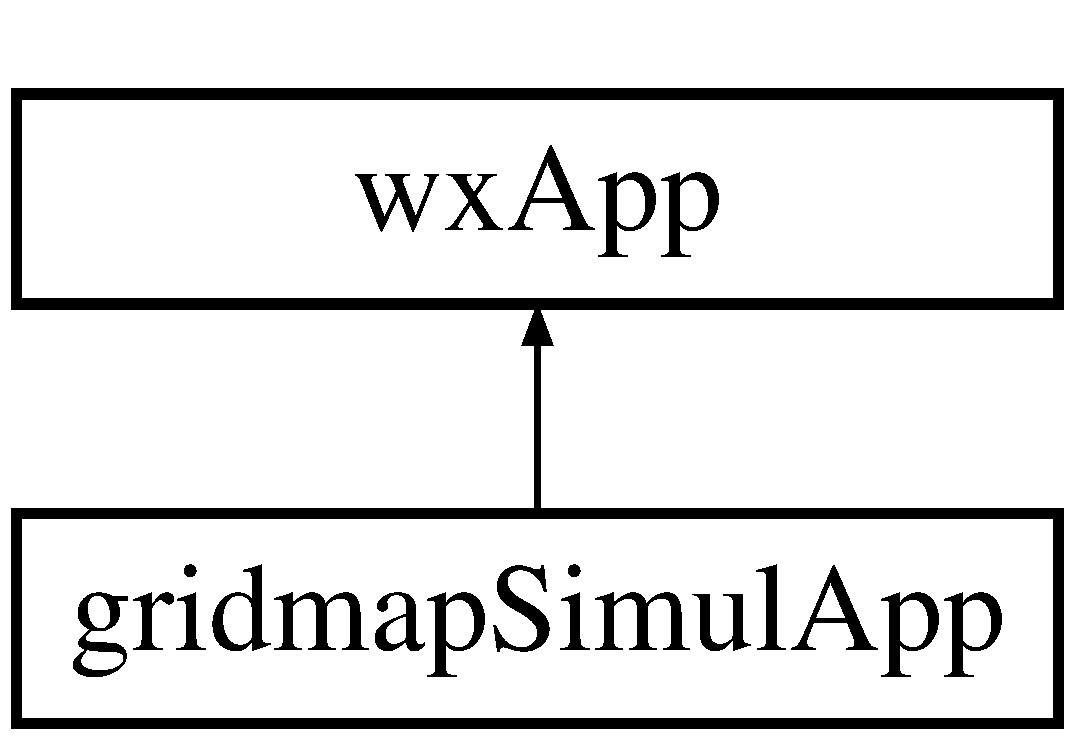
\includegraphics[height=2.000000cm]{classgridmapSimulApp}
\end{center}
\end{figure}
\subsection*{Public Member Functions}
\begin{DoxyCompactItemize}
\item 
\mbox{\Hypertarget{classgridmapSimulApp_abc43c8f695eb785e35a33f72ac180321}\label{classgridmapSimulApp_abc43c8f695eb785e35a33f72ac180321}} 
virtual bool {\bfseries On\+Init} ()
\item 
\mbox{\Hypertarget{classgridmapSimulApp_a4f8e8dc4a836ed655bde844103969e68}\label{classgridmapSimulApp_a4f8e8dc4a836ed655bde844103969e68}} 
virtual int {\bfseries On\+Exit} ()
\end{DoxyCompactItemize}


The documentation for this class was generated from the following files\+:\begin{DoxyCompactItemize}
\item 
gridmap\+Simul\+App.\+h\item 
gridmap\+Simul\+App.\+cpp\end{DoxyCompactItemize}

\hypertarget{classgridmapSimulFrame}{}\section{gridmap\+Simul\+Frame Class Reference}
\label{classgridmapSimulFrame}\index{gridmap\+Simul\+Frame@{gridmap\+Simul\+Frame}}
Inheritance diagram for gridmap\+Simul\+Frame\+:\begin{figure}[H]
\begin{center}
\leavevmode
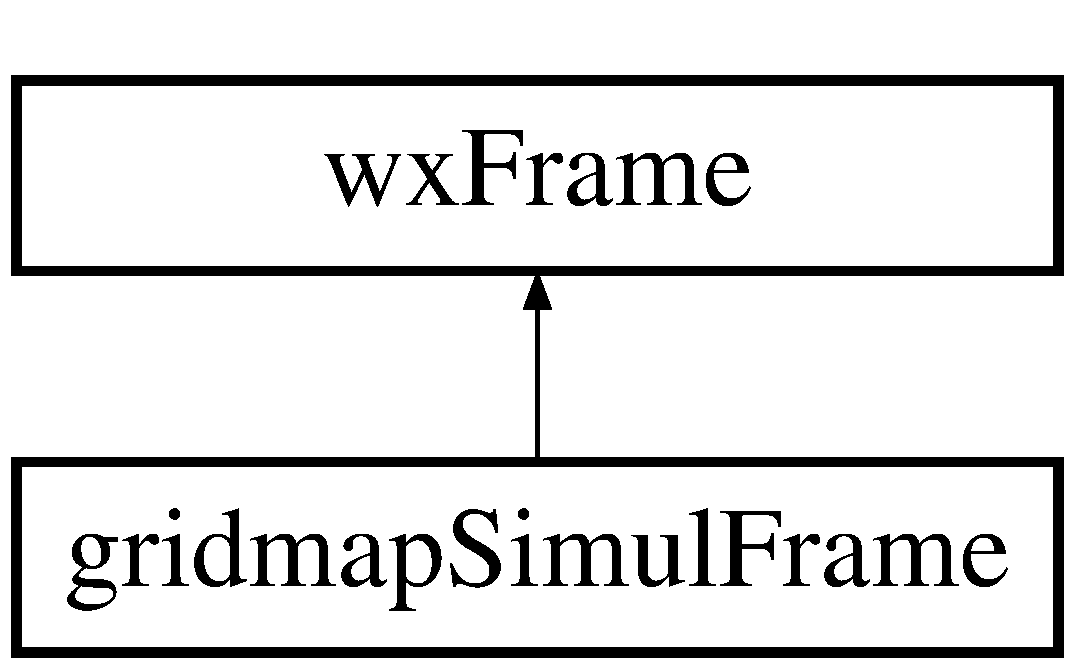
\includegraphics[height=2.000000cm]{classgridmapSimulFrame}
\end{center}
\end{figure}
\subsection*{Public Member Functions}
\begin{DoxyCompactItemize}
\item 
\mbox{\Hypertarget{classgridmapSimulFrame_ac1ac89ea6a9a31594031b1555124e9de}\label{classgridmapSimulFrame_ac1ac89ea6a9a31594031b1555124e9de}} 
{\bfseries gridmap\+Simul\+Frame} (wx\+Window $\ast$parent, wx\+Window\+ID id=-\/1)
\end{DoxyCompactItemize}


The documentation for this class was generated from the following files\+:\begin{DoxyCompactItemize}
\item 
gridmap\+Simul\+Main.\+h\item 
gridmap\+Simul\+Main.\+cpp\end{DoxyCompactItemize}

\hypertarget{classMyArtProvider}{}\section{My\+Art\+Provider Class Reference}
\label{classMyArtProvider}\index{My\+Art\+Provider@{My\+Art\+Provider}}
Inheritance diagram for My\+Art\+Provider\+:\begin{figure}[H]
\begin{center}
\leavevmode
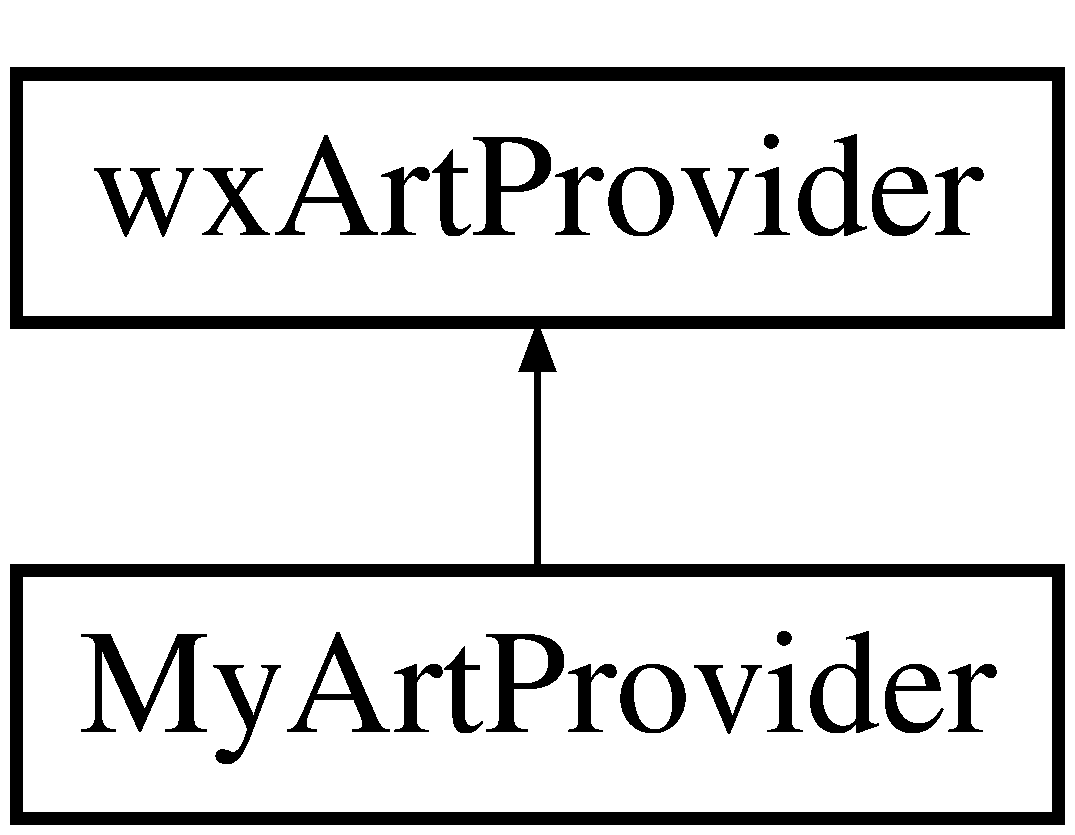
\includegraphics[height=2.000000cm]{classMyArtProvider}
\end{center}
\end{figure}
\subsection*{Protected Member Functions}
\begin{DoxyCompactItemize}
\item 
\mbox{\Hypertarget{classMyArtProvider_a4f06bcde38b57c560d5d9ec79ebd35dc}\label{classMyArtProvider_a4f06bcde38b57c560d5d9ec79ebd35dc}} 
virtual wx\+Bitmap {\bfseries Create\+Bitmap} (const wx\+Art\+ID \&id, const wx\+Art\+Client \&client, const wx\+Size \&size)
\end{DoxyCompactItemize}


\subsection{Detailed Description}
\#include \char`\"{}virtual\+\_\+map1.\+xpm\char`\"{} include \char`\"{}map2.\+xpm\char`\"{} include \char`\"{}map3.\+xpm\char`\"{} include \char`\"{}map3pro.\+xpm\char`\"{} \#include \char`\"{}map3pro\+\_\+mini\+\_\+xpm\char`\"{} include \char`\"{}map3pro\+\_\+mini2.\+xpm\char`\"{} 

The documentation for this class was generated from the following file\+:\begin{DoxyCompactItemize}
\item 
gridmap\+Simul\+Main.\+cpp\end{DoxyCompactItemize}

\hypertarget{structmotion_1_1TMotion}{}\section{motion\+:\+:T\+Motion Struct Reference}
\label{structmotion_1_1TMotion}\index{motion\+::\+T\+Motion@{motion\+::\+T\+Motion}}


{\ttfamily \#include $<$T\+Motion.\+h$>$}

\subsection*{Public Member Functions}
\begin{DoxyCompactItemize}
\item 
\mbox{\Hypertarget{structmotion_1_1TMotion_a28732b6329e66119a212467bba34cc36}\label{structmotion_1_1TMotion_a28732b6329e66119a212467bba34cc36}} 
void {\bfseries init} (void)
\end{DoxyCompactItemize}
\subsection*{Public Attributes}
\begin{DoxyCompactItemize}
\item 
double \mbox{\hyperlink{structmotion_1_1TMotion_aeda5c209f0c5d82440b41c677d3ea529}{linear\+Velocity}}
\item 
double \mbox{\hyperlink{structmotion_1_1TMotion_afe8d2e8d60f8792e3910f52247d63cdc}{angular\+Velocity}}
\item 
double \mbox{\hyperlink{structmotion_1_1TMotion_a17243eb4c7f2ea4f52532ca537f51fc4}{side\+Dist}}
\item 
double \mbox{\hyperlink{structmotion_1_1TMotion_a367ffdd10f1094a1f263cbb43f341cd8}{ahead\+Dist}}
\item 
double \mbox{\hyperlink{structmotion_1_1TMotion_a927510756a7eb9cacae2fcea8ded4dc5}{time\+Needed}}
\item 
double \mbox{\hyperlink{structmotion_1_1TMotion_a9666f9ac141497a4fe324431c24b2f16}{pre\+Phi}}
\item 
bool \mbox{\hyperlink{structmotion_1_1TMotion_a1e5e34bc2826af1f1655ef0e57d598c7}{positive\+Set}}
\item 
\mbox{\hyperlink{motionEnums_8h_a03a5344cd29a761a4b7dcaf1df3c3c85}{E\+Rotate\+Side}} \mbox{\hyperlink{structmotion_1_1TMotion_ad1c88e25a3f1e71b94e6173a64f6212a}{positive}}
\item 
int \mbox{\hyperlink{structmotion_1_1TMotion_a9080c7c722cd68cab5ecd832e2ceca82}{jump\+Count}}
\item 
\mbox{\hyperlink{motionEnums_8h_a03a5344cd29a761a4b7dcaf1df3c3c85}{E\+Rotate\+Side}} \mbox{\hyperlink{structmotion_1_1TMotion_a2b174cdd1ddccc5fc08d04f074a45686}{jump\+Direction}}
\item 
\mbox{\hyperlink{motionEnums_8h_a183cd5b7c370a05cb3b44fb54e0fee66}{E\+P\+T\+Mode}} \mbox{\hyperlink{structmotion_1_1TMotion_afbcc18b70d7d5b75906addd67e698bbf}{pt\+Mode}}
\item 
bool \mbox{\hyperlink{structmotion_1_1TMotion_a138af2063ec400b8031da3cb019d4723}{pose\+Stored}}
\item 
\mbox{\hyperlink{structmotion_1_1TMotionPose2D}{T\+Motion\+Pose2D}} \mbox{\hyperlink{structmotion_1_1TMotion_a9fbd5c971ef085ed45054abd82b650eb}{start\+Pose}}
\item 
\mbox{\hyperlink{structmotion_1_1TMotionPose2D}{T\+Motion\+Pose2D}} \mbox{\hyperlink{structmotion_1_1TMotion_a19c4b369e9e8c9c290a86a1a4ead53a0}{cur\+Pose}}
\item 
\mbox{\hyperlink{motionEnums_8h_a907f80786f402332d43f4646dc1450bc}{E\+Motion}} \mbox{\hyperlink{structmotion_1_1TMotion_afd2a57c061f52c0e506ab9fba29558e4}{mot}}
\item 
\mbox{\hyperlink{motionEnums_8h_a23be5ef75af9219a8bf688fd9716d72c}{E\+Sub\+Motion}} \mbox{\hyperlink{structmotion_1_1TMotion_a5e9becca4a1f88a70dd4b97c65b737de}{sub\+Mot}}
\item 
\mbox{\hyperlink{motionEnums_8h_a272f94c6143b9acf7ac44f165be53948}{E\+Sub\+Motion\+State}} \mbox{\hyperlink{structmotion_1_1TMotion_a867be2dd284ef064809db4e384a722b2}{sub\+Mot\+State}}
\item 
\mbox{\hyperlink{motionEnums_8h_aa7486027d362655230b958efe6985a7f}{E\+Action}} \mbox{\hyperlink{structmotion_1_1TMotion_ac51f74a01dd87aacda81c14028a80ccf}{act}}
\item 
\mbox{\hyperlink{motionEnums_8h_ac80e838bea11b75469bfc14b1de921a3}{E\+Action\+State}} \mbox{\hyperlink{structmotion_1_1TMotion_a87ff7f273ed899eb720d3ef7ef8fe543}{act\+State}}
\item 
\mbox{\hyperlink{structmotion_1_1TMotionParams}{T\+Motion\+Params}} \mbox{\hyperlink{structmotion_1_1TMotion_a67eb890fbd74ee1c88a5d640a199dea4}{mot\+Params}}
\end{DoxyCompactItemize}


\subsection{Detailed Description}
Motion shared parameters ~\newline


\subsection{Member Data Documentation}
\mbox{\Hypertarget{structmotion_1_1TMotion_ac51f74a01dd87aacda81c14028a80ccf}\label{structmotion_1_1TMotion_ac51f74a01dd87aacda81c14028a80ccf}} 
\index{motion\+::\+T\+Motion@{motion\+::\+T\+Motion}!act@{act}}
\index{act@{act}!motion\+::\+T\+Motion@{motion\+::\+T\+Motion}}
\subsubsection{\texorpdfstring{act}{act}}
{\footnotesize\ttfamily \mbox{\hyperlink{motionEnums_8h_aa7486027d362655230b958efe6985a7f}{E\+Action}} motion\+::\+T\+Motion\+::act}

Current action. \mbox{\Hypertarget{structmotion_1_1TMotion_a87ff7f273ed899eb720d3ef7ef8fe543}\label{structmotion_1_1TMotion_a87ff7f273ed899eb720d3ef7ef8fe543}} 
\index{motion\+::\+T\+Motion@{motion\+::\+T\+Motion}!act\+State@{act\+State}}
\index{act\+State@{act\+State}!motion\+::\+T\+Motion@{motion\+::\+T\+Motion}}
\subsubsection{\texorpdfstring{act\+State}{actState}}
{\footnotesize\ttfamily \mbox{\hyperlink{motionEnums_8h_ac80e838bea11b75469bfc14b1de921a3}{E\+Action\+State}} motion\+::\+T\+Motion\+::act\+State}

Current action state. \mbox{\Hypertarget{structmotion_1_1TMotion_a367ffdd10f1094a1f263cbb43f341cd8}\label{structmotion_1_1TMotion_a367ffdd10f1094a1f263cbb43f341cd8}} 
\index{motion\+::\+T\+Motion@{motion\+::\+T\+Motion}!ahead\+Dist@{ahead\+Dist}}
\index{ahead\+Dist@{ahead\+Dist}!motion\+::\+T\+Motion@{motion\+::\+T\+Motion}}
\subsubsection{\texorpdfstring{ahead\+Dist}{aheadDist}}
{\footnotesize\ttfamily double motion\+::\+T\+Motion\+::ahead\+Dist}

The ahead distance. \mbox{\Hypertarget{structmotion_1_1TMotion_afe8d2e8d60f8792e3910f52247d63cdc}\label{structmotion_1_1TMotion_afe8d2e8d60f8792e3910f52247d63cdc}} 
\index{motion\+::\+T\+Motion@{motion\+::\+T\+Motion}!angular\+Velocity@{angular\+Velocity}}
\index{angular\+Velocity@{angular\+Velocity}!motion\+::\+T\+Motion@{motion\+::\+T\+Motion}}
\subsubsection{\texorpdfstring{angular\+Velocity}{angularVelocity}}
{\footnotesize\ttfamily double motion\+::\+T\+Motion\+::angular\+Velocity}

Angular velocity of the robot. \mbox{\Hypertarget{structmotion_1_1TMotion_a19c4b369e9e8c9c290a86a1a4ead53a0}\label{structmotion_1_1TMotion_a19c4b369e9e8c9c290a86a1a4ead53a0}} 
\index{motion\+::\+T\+Motion@{motion\+::\+T\+Motion}!cur\+Pose@{cur\+Pose}}
\index{cur\+Pose@{cur\+Pose}!motion\+::\+T\+Motion@{motion\+::\+T\+Motion}}
\subsubsection{\texorpdfstring{cur\+Pose}{curPose}}
{\footnotesize\ttfamily \mbox{\hyperlink{structmotion_1_1TMotionPose2D}{T\+Motion\+Pose2D}} motion\+::\+T\+Motion\+::cur\+Pose}

Current pose. \mbox{\Hypertarget{structmotion_1_1TMotion_a9080c7c722cd68cab5ecd832e2ceca82}\label{structmotion_1_1TMotion_a9080c7c722cd68cab5ecd832e2ceca82}} 
\index{motion\+::\+T\+Motion@{motion\+::\+T\+Motion}!jump\+Count@{jump\+Count}}
\index{jump\+Count@{jump\+Count}!motion\+::\+T\+Motion@{motion\+::\+T\+Motion}}
\subsubsection{\texorpdfstring{jump\+Count}{jumpCount}}
{\footnotesize\ttfamily int motion\+::\+T\+Motion\+::jump\+Count}

Jump count. Jump is defined as the robot rotated -\/180-\/$>$180 or 180-\/$>$-\/180. \mbox{\Hypertarget{structmotion_1_1TMotion_a2b174cdd1ddccc5fc08d04f074a45686}\label{structmotion_1_1TMotion_a2b174cdd1ddccc5fc08d04f074a45686}} 
\index{motion\+::\+T\+Motion@{motion\+::\+T\+Motion}!jump\+Direction@{jump\+Direction}}
\index{jump\+Direction@{jump\+Direction}!motion\+::\+T\+Motion@{motion\+::\+T\+Motion}}
\subsubsection{\texorpdfstring{jump\+Direction}{jumpDirection}}
{\footnotesize\ttfamily \mbox{\hyperlink{motionEnums_8h_a03a5344cd29a761a4b7dcaf1df3c3c85}{E\+Rotate\+Side}} motion\+::\+T\+Motion\+::jump\+Direction}

Jump direction. \mbox{\Hypertarget{structmotion_1_1TMotion_aeda5c209f0c5d82440b41c677d3ea529}\label{structmotion_1_1TMotion_aeda5c209f0c5d82440b41c677d3ea529}} 
\index{motion\+::\+T\+Motion@{motion\+::\+T\+Motion}!linear\+Velocity@{linear\+Velocity}}
\index{linear\+Velocity@{linear\+Velocity}!motion\+::\+T\+Motion@{motion\+::\+T\+Motion}}
\subsubsection{\texorpdfstring{linear\+Velocity}{linearVelocity}}
{\footnotesize\ttfamily double motion\+::\+T\+Motion\+::linear\+Velocity}

Linear velocity of the robot. \mbox{\Hypertarget{structmotion_1_1TMotion_afd2a57c061f52c0e506ab9fba29558e4}\label{structmotion_1_1TMotion_afd2a57c061f52c0e506ab9fba29558e4}} 
\index{motion\+::\+T\+Motion@{motion\+::\+T\+Motion}!mot@{mot}}
\index{mot@{mot}!motion\+::\+T\+Motion@{motion\+::\+T\+Motion}}
\subsubsection{\texorpdfstring{mot}{mot}}
{\footnotesize\ttfamily \mbox{\hyperlink{motionEnums_8h_a907f80786f402332d43f4646dc1450bc}{E\+Motion}} motion\+::\+T\+Motion\+::mot}

Current motion \mbox{\Hypertarget{structmotion_1_1TMotion_a67eb890fbd74ee1c88a5d640a199dea4}\label{structmotion_1_1TMotion_a67eb890fbd74ee1c88a5d640a199dea4}} 
\index{motion\+::\+T\+Motion@{motion\+::\+T\+Motion}!mot\+Params@{mot\+Params}}
\index{mot\+Params@{mot\+Params}!motion\+::\+T\+Motion@{motion\+::\+T\+Motion}}
\subsubsection{\texorpdfstring{mot\+Params}{motParams}}
{\footnotesize\ttfamily \mbox{\hyperlink{structmotion_1_1TMotionParams}{T\+Motion\+Params}} motion\+::\+T\+Motion\+::mot\+Params}

Motion related parameters. \mbox{\Hypertarget{structmotion_1_1TMotion_a138af2063ec400b8031da3cb019d4723}\label{structmotion_1_1TMotion_a138af2063ec400b8031da3cb019d4723}} 
\index{motion\+::\+T\+Motion@{motion\+::\+T\+Motion}!pose\+Stored@{pose\+Stored}}
\index{pose\+Stored@{pose\+Stored}!motion\+::\+T\+Motion@{motion\+::\+T\+Motion}}
\subsubsection{\texorpdfstring{pose\+Stored}{poseStored}}
{\footnotesize\ttfamily bool motion\+::\+T\+Motion\+::pose\+Stored}

Pose stored mark. \mbox{\Hypertarget{structmotion_1_1TMotion_ad1c88e25a3f1e71b94e6173a64f6212a}\label{structmotion_1_1TMotion_ad1c88e25a3f1e71b94e6173a64f6212a}} 
\index{motion\+::\+T\+Motion@{motion\+::\+T\+Motion}!positive@{positive}}
\index{positive@{positive}!motion\+::\+T\+Motion@{motion\+::\+T\+Motion}}
\subsubsection{\texorpdfstring{positive}{positive}}
{\footnotesize\ttfamily \mbox{\hyperlink{motionEnums_8h_a03a5344cd29a761a4b7dcaf1df3c3c85}{E\+Rotate\+Side}} motion\+::\+T\+Motion\+::positive}

The positive direction when rotating. \mbox{\Hypertarget{structmotion_1_1TMotion_a1e5e34bc2826af1f1655ef0e57d598c7}\label{structmotion_1_1TMotion_a1e5e34bc2826af1f1655ef0e57d598c7}} 
\index{motion\+::\+T\+Motion@{motion\+::\+T\+Motion}!positive\+Set@{positive\+Set}}
\index{positive\+Set@{positive\+Set}!motion\+::\+T\+Motion@{motion\+::\+T\+Motion}}
\subsubsection{\texorpdfstring{positive\+Set}{positiveSet}}
{\footnotesize\ttfamily bool motion\+::\+T\+Motion\+::positive\+Set}

The positive-\/direction-\/set mark \mbox{\Hypertarget{structmotion_1_1TMotion_a9666f9ac141497a4fe324431c24b2f16}\label{structmotion_1_1TMotion_a9666f9ac141497a4fe324431c24b2f16}} 
\index{motion\+::\+T\+Motion@{motion\+::\+T\+Motion}!pre\+Phi@{pre\+Phi}}
\index{pre\+Phi@{pre\+Phi}!motion\+::\+T\+Motion@{motion\+::\+T\+Motion}}
\subsubsection{\texorpdfstring{pre\+Phi}{prePhi}}
{\footnotesize\ttfamily double motion\+::\+T\+Motion\+::pre\+Phi}

Previous phi. \mbox{\Hypertarget{structmotion_1_1TMotion_afbcc18b70d7d5b75906addd67e698bbf}\label{structmotion_1_1TMotion_afbcc18b70d7d5b75906addd67e698bbf}} 
\index{motion\+::\+T\+Motion@{motion\+::\+T\+Motion}!pt\+Mode@{pt\+Mode}}
\index{pt\+Mode@{pt\+Mode}!motion\+::\+T\+Motion@{motion\+::\+T\+Motion}}
\subsubsection{\texorpdfstring{pt\+Mode}{ptMode}}
{\footnotesize\ttfamily \mbox{\hyperlink{motionEnums_8h_a183cd5b7c370a05cb3b44fb54e0fee66}{E\+P\+T\+Mode}} motion\+::\+T\+Motion\+::pt\+Mode}

The point tracking mode. A\+PT\+: arc point tracking, L\+PT\+: linear point tracking. \mbox{\Hypertarget{structmotion_1_1TMotion_a17243eb4c7f2ea4f52532ca537f51fc4}\label{structmotion_1_1TMotion_a17243eb4c7f2ea4f52532ca537f51fc4}} 
\index{motion\+::\+T\+Motion@{motion\+::\+T\+Motion}!side\+Dist@{side\+Dist}}
\index{side\+Dist@{side\+Dist}!motion\+::\+T\+Motion@{motion\+::\+T\+Motion}}
\subsubsection{\texorpdfstring{side\+Dist}{sideDist}}
{\footnotesize\ttfamily double motion\+::\+T\+Motion\+::side\+Dist}

The side distance. \mbox{\Hypertarget{structmotion_1_1TMotion_a9fbd5c971ef085ed45054abd82b650eb}\label{structmotion_1_1TMotion_a9fbd5c971ef085ed45054abd82b650eb}} 
\index{motion\+::\+T\+Motion@{motion\+::\+T\+Motion}!start\+Pose@{start\+Pose}}
\index{start\+Pose@{start\+Pose}!motion\+::\+T\+Motion@{motion\+::\+T\+Motion}}
\subsubsection{\texorpdfstring{start\+Pose}{startPose}}
{\footnotesize\ttfamily \mbox{\hyperlink{structmotion_1_1TMotionPose2D}{T\+Motion\+Pose2D}} motion\+::\+T\+Motion\+::start\+Pose}

Start pose. \mbox{\Hypertarget{structmotion_1_1TMotion_a5e9becca4a1f88a70dd4b97c65b737de}\label{structmotion_1_1TMotion_a5e9becca4a1f88a70dd4b97c65b737de}} 
\index{motion\+::\+T\+Motion@{motion\+::\+T\+Motion}!sub\+Mot@{sub\+Mot}}
\index{sub\+Mot@{sub\+Mot}!motion\+::\+T\+Motion@{motion\+::\+T\+Motion}}
\subsubsection{\texorpdfstring{sub\+Mot}{subMot}}
{\footnotesize\ttfamily \mbox{\hyperlink{motionEnums_8h_a23be5ef75af9219a8bf688fd9716d72c}{E\+Sub\+Motion}} motion\+::\+T\+Motion\+::sub\+Mot}

Current sub-\/motion. \mbox{\Hypertarget{structmotion_1_1TMotion_a867be2dd284ef064809db4e384a722b2}\label{structmotion_1_1TMotion_a867be2dd284ef064809db4e384a722b2}} 
\index{motion\+::\+T\+Motion@{motion\+::\+T\+Motion}!sub\+Mot\+State@{sub\+Mot\+State}}
\index{sub\+Mot\+State@{sub\+Mot\+State}!motion\+::\+T\+Motion@{motion\+::\+T\+Motion}}
\subsubsection{\texorpdfstring{sub\+Mot\+State}{subMotState}}
{\footnotesize\ttfamily \mbox{\hyperlink{motionEnums_8h_a272f94c6143b9acf7ac44f165be53948}{E\+Sub\+Motion\+State}} motion\+::\+T\+Motion\+::sub\+Mot\+State}

Current Sub-\/motion state. \mbox{\Hypertarget{structmotion_1_1TMotion_a927510756a7eb9cacae2fcea8ded4dc5}\label{structmotion_1_1TMotion_a927510756a7eb9cacae2fcea8ded4dc5}} 
\index{motion\+::\+T\+Motion@{motion\+::\+T\+Motion}!time\+Needed@{time\+Needed}}
\index{time\+Needed@{time\+Needed}!motion\+::\+T\+Motion@{motion\+::\+T\+Motion}}
\subsubsection{\texorpdfstring{time\+Needed}{timeNeeded}}
{\footnotesize\ttfamily double motion\+::\+T\+Motion\+::time\+Needed}

Time needed to finished the task. 

The documentation for this struct was generated from the following file\+:\begin{DoxyCompactItemize}
\item 
motion/misc/\mbox{\hyperlink{TMotion_8h}{T\+Motion.\+h}}\end{DoxyCompactItemize}

\hypertarget{structmotion_1_1TMotionParams}{}\section{motion\+:\+:T\+Motion\+Params Struct Reference}
\label{structmotion_1_1TMotionParams}\index{motion\+::\+T\+Motion\+Params@{motion\+::\+T\+Motion\+Params}}


{\ttfamily \#include $<$T\+Motion\+Params.\+h$>$}

\subsection*{Public Member Functions}
\begin{DoxyCompactItemize}
\item 
\mbox{\Hypertarget{structmotion_1_1TMotionParams_a0161219617053bae842f1ce93b555c12}\label{structmotion_1_1TMotionParams_a0161219617053bae842f1ce93b555c12}} 
{\bfseries T\+Motion\+Params} (double x=0.\+0, double y=0.\+0, \mbox{\hyperlink{motionEnums_8h_a183cd5b7c370a05cb3b44fb54e0fee66}{E\+P\+T\+Mode}} m=L\+PT, \mbox{\hyperlink{motionEnums_8h_a203932f574f7edf20737611293eecaa3}{E\+P\+T\+Bump\+Mode}} bm=F\+R\+A\+G\+I\+LE, double v=wall\+FolV, double dist=wall\+Fol\+Side\+Dist)
\item 
\mbox{\Hypertarget{structmotion_1_1TMotionParams_a9a8b167a486d5850503e1c850311dac4}\label{structmotion_1_1TMotionParams_a9a8b167a486d5850503e1c850311dac4}} 
void {\bfseries reset} (void)
\item 
\mbox{\Hypertarget{structmotion_1_1TMotionParams_a20e1399cfa1c1a494018415a912845be}\label{structmotion_1_1TMotionParams_a20e1399cfa1c1a494018415a912845be}} 
const \mbox{\hyperlink{structmotion_1_1TMotionParams}{T\+Motion\+Params}} \& {\bfseries operator=} (const \mbox{\hyperlink{structmotion_1_1TMotionParams}{T\+Motion\+Params}} \&rhs)
\end{DoxyCompactItemize}
\subsection*{Public Attributes}
\begin{DoxyCompactItemize}
\item 
\mbox{\hyperlink{structmotion_1_1TMotionPose2D}{T\+Motion\+Pose2D}} \mbox{\hyperlink{structmotion_1_1TMotionParams_aa2a166593403a7d673854c2243676e88}{P\+T\+\_\+loc}}
\item 
\mbox{\hyperlink{motionEnums_8h_a183cd5b7c370a05cb3b44fb54e0fee66}{E\+P\+T\+Mode}} \mbox{\hyperlink{structmotion_1_1TMotionParams_a18e01529102e9029f4f5606e0d129847}{P\+T\+\_\+mode}}
\item 
\mbox{\hyperlink{motionEnums_8h_a203932f574f7edf20737611293eecaa3}{E\+P\+T\+Bump\+Mode}} \mbox{\hyperlink{structmotion_1_1TMotionParams_a2bfcdc11525a62ab3b47ced208c5e44e}{P\+T\+\_\+bump\+Mode}}
\item 
double \mbox{\hyperlink{structmotion_1_1TMotionParams_ab9825758467d9ed3b06efeb705ad4572}{W\+F\+\_\+V}}
\item 
double \mbox{\hyperlink{structmotion_1_1TMotionParams_a821918ccf43fc2a6980945a2f9806257}{W\+F\+\_\+dist}}
\end{DoxyCompactItemize}


\subsection{Detailed Description}
Motion settable parameters ~\newline


\subsection{Member Data Documentation}
\mbox{\Hypertarget{structmotion_1_1TMotionParams_a2bfcdc11525a62ab3b47ced208c5e44e}\label{structmotion_1_1TMotionParams_a2bfcdc11525a62ab3b47ced208c5e44e}} 
\index{motion\+::\+T\+Motion\+Params@{motion\+::\+T\+Motion\+Params}!P\+T\+\_\+bump\+Mode@{P\+T\+\_\+bump\+Mode}}
\index{P\+T\+\_\+bump\+Mode@{P\+T\+\_\+bump\+Mode}!motion\+::\+T\+Motion\+Params@{motion\+::\+T\+Motion\+Params}}
\subsubsection{\texorpdfstring{P\+T\+\_\+bump\+Mode}{PT\_bumpMode}}
{\footnotesize\ttfamily \mbox{\hyperlink{motionEnums_8h_a203932f574f7edf20737611293eecaa3}{E\+P\+T\+Bump\+Mode}} motion\+::\+T\+Motion\+Params\+::\+P\+T\+\_\+bump\+Mode}

Bump mode\+: fragile or strong. \mbox{\Hypertarget{structmotion_1_1TMotionParams_aa2a166593403a7d673854c2243676e88}\label{structmotion_1_1TMotionParams_aa2a166593403a7d673854c2243676e88}} 
\index{motion\+::\+T\+Motion\+Params@{motion\+::\+T\+Motion\+Params}!P\+T\+\_\+loc@{P\+T\+\_\+loc}}
\index{P\+T\+\_\+loc@{P\+T\+\_\+loc}!motion\+::\+T\+Motion\+Params@{motion\+::\+T\+Motion\+Params}}
\subsubsection{\texorpdfstring{P\+T\+\_\+loc}{PT\_loc}}
{\footnotesize\ttfamily \mbox{\hyperlink{structmotion_1_1TMotionPose2D}{T\+Motion\+Pose2D}} motion\+::\+T\+Motion\+Params\+::\+P\+T\+\_\+loc}

Target location. \mbox{\Hypertarget{structmotion_1_1TMotionParams_a18e01529102e9029f4f5606e0d129847}\label{structmotion_1_1TMotionParams_a18e01529102e9029f4f5606e0d129847}} 
\index{motion\+::\+T\+Motion\+Params@{motion\+::\+T\+Motion\+Params}!P\+T\+\_\+mode@{P\+T\+\_\+mode}}
\index{P\+T\+\_\+mode@{P\+T\+\_\+mode}!motion\+::\+T\+Motion\+Params@{motion\+::\+T\+Motion\+Params}}
\subsubsection{\texorpdfstring{P\+T\+\_\+mode}{PT\_mode}}
{\footnotesize\ttfamily \mbox{\hyperlink{motionEnums_8h_a183cd5b7c370a05cb3b44fb54e0fee66}{E\+P\+T\+Mode}} motion\+::\+T\+Motion\+Params\+::\+P\+T\+\_\+mode}

Point tracking mode\+: L\+P\+T(linear) or A\+P\+T(arc). \mbox{\Hypertarget{structmotion_1_1TMotionParams_a821918ccf43fc2a6980945a2f9806257}\label{structmotion_1_1TMotionParams_a821918ccf43fc2a6980945a2f9806257}} 
\index{motion\+::\+T\+Motion\+Params@{motion\+::\+T\+Motion\+Params}!W\+F\+\_\+dist@{W\+F\+\_\+dist}}
\index{W\+F\+\_\+dist@{W\+F\+\_\+dist}!motion\+::\+T\+Motion\+Params@{motion\+::\+T\+Motion\+Params}}
\subsubsection{\texorpdfstring{W\+F\+\_\+dist}{WF\_dist}}
{\footnotesize\ttfamily double motion\+::\+T\+Motion\+Params\+::\+W\+F\+\_\+dist}

Wall following side distance. \mbox{\Hypertarget{structmotion_1_1TMotionParams_ab9825758467d9ed3b06efeb705ad4572}\label{structmotion_1_1TMotionParams_ab9825758467d9ed3b06efeb705ad4572}} 
\index{motion\+::\+T\+Motion\+Params@{motion\+::\+T\+Motion\+Params}!W\+F\+\_\+V@{W\+F\+\_\+V}}
\index{W\+F\+\_\+V@{W\+F\+\_\+V}!motion\+::\+T\+Motion\+Params@{motion\+::\+T\+Motion\+Params}}
\subsubsection{\texorpdfstring{W\+F\+\_\+V}{WF\_V}}
{\footnotesize\ttfamily double motion\+::\+T\+Motion\+Params\+::\+W\+F\+\_\+V}

Wall following linear velocity. 

The documentation for this struct was generated from the following file\+:\begin{DoxyCompactItemize}
\item 
motion/misc/\mbox{\hyperlink{TMotionParams_8h}{T\+Motion\+Params.\+h}}\end{DoxyCompactItemize}

\hypertarget{structTMotionPIDCon}{}\section{T\+Motion\+P\+I\+D\+Con Struct Reference}
\label{structTMotionPIDCon}\index{T\+Motion\+P\+I\+D\+Con@{T\+Motion\+P\+I\+D\+Con}}
\subsection*{Public Member Functions}
\begin{DoxyCompactItemize}
\item 
\mbox{\hyperlink{structTMotionPIDCon_a89a9b1ec1b91eb7ea5b3dd9f3dd38d92}{T\+Motion\+P\+I\+D\+Con}} (double kp, double ki, double kd=0)
\item 
double \mbox{\hyperlink{structTMotionPIDCon_a138ff107e0fece2fd74a1fed606261ae}{pid}} (double err)
\end{DoxyCompactItemize}
\subsection*{Public Attributes}
\begin{DoxyCompactItemize}
\item 
double \mbox{\hyperlink{structTMotionPIDCon_ac8a816dbcf1f644c140dbd2f7b8df58d}{m\+\_\+kP}}
\item 
double \mbox{\hyperlink{structTMotionPIDCon_ac8192a3af9ef9f350128f34c276ce493}{m\+\_\+kI}}
\item 
double \mbox{\hyperlink{structTMotionPIDCon_a07e1da9c56d8153c6c576bb8b533a80d}{m\+\_\+kD}}
\item 
double \mbox{\hyperlink{structTMotionPIDCon_ac048b1ed8486f28e941648bc0518695a}{m\+\_\+il}}
\item 
double \mbox{\hyperlink{structTMotionPIDCon_a51de95c7d07b1bf075d5e5834671506a}{m\+\_\+output}}
\item 
double \mbox{\hyperlink{structTMotionPIDCon_ad7b4b7d9804f5130511442b8f1543d09}{m\+\_\+inte\+Err}}
\item 
double \mbox{\hyperlink{structTMotionPIDCon_a70da1dcf5bae866184f047980ef4eae2}{m\+\_\+delta\+Err}}
\item 
double \mbox{\hyperlink{structTMotionPIDCon_a319c2f863bb3965d8caaa008e2e1bd87}{m\+\_\+pre\+Err}}
\end{DoxyCompactItemize}


\subsection{Constructor \& Destructor Documentation}
\mbox{\Hypertarget{structTMotionPIDCon_a89a9b1ec1b91eb7ea5b3dd9f3dd38d92}\label{structTMotionPIDCon_a89a9b1ec1b91eb7ea5b3dd9f3dd38d92}} 
\index{T\+Motion\+P\+I\+D\+Con@{T\+Motion\+P\+I\+D\+Con}!T\+Motion\+P\+I\+D\+Con@{T\+Motion\+P\+I\+D\+Con}}
\index{T\+Motion\+P\+I\+D\+Con@{T\+Motion\+P\+I\+D\+Con}!T\+Motion\+P\+I\+D\+Con@{T\+Motion\+P\+I\+D\+Con}}
\subsubsection{\texorpdfstring{T\+Motion\+P\+I\+D\+Con()}{TMotionPIDCon()}}
{\footnotesize\ttfamily T\+Motion\+P\+I\+D\+Con\+::\+T\+Motion\+P\+I\+D\+Con (\begin{DoxyParamCaption}\item[{double}]{kp,  }\item[{double}]{ki,  }\item[{double}]{kd = {\ttfamily 0} }\end{DoxyParamCaption})\hspace{0.3cm}{\ttfamily [inline]}}

Constructor 

\subsection{Member Function Documentation}
\mbox{\Hypertarget{structTMotionPIDCon_a138ff107e0fece2fd74a1fed606261ae}\label{structTMotionPIDCon_a138ff107e0fece2fd74a1fed606261ae}} 
\index{T\+Motion\+P\+I\+D\+Con@{T\+Motion\+P\+I\+D\+Con}!pid@{pid}}
\index{pid@{pid}!T\+Motion\+P\+I\+D\+Con@{T\+Motion\+P\+I\+D\+Con}}
\subsubsection{\texorpdfstring{pid()}{pid()}}
{\footnotesize\ttfamily double T\+Motion\+P\+I\+D\+Con\+::pid (\begin{DoxyParamCaption}\item[{double}]{err }\end{DoxyParamCaption})\hspace{0.3cm}{\ttfamily [inline]}}

Controller if(m\+\_\+inte\+Err $>$= m\+\_\+il) \{ m\+\_\+inte\+Err = m\+\_\+il; \} 

\subsection{Member Data Documentation}
\mbox{\Hypertarget{structTMotionPIDCon_a70da1dcf5bae866184f047980ef4eae2}\label{structTMotionPIDCon_a70da1dcf5bae866184f047980ef4eae2}} 
\index{T\+Motion\+P\+I\+D\+Con@{T\+Motion\+P\+I\+D\+Con}!m\+\_\+delta\+Err@{m\+\_\+delta\+Err}}
\index{m\+\_\+delta\+Err@{m\+\_\+delta\+Err}!T\+Motion\+P\+I\+D\+Con@{T\+Motion\+P\+I\+D\+Con}}
\subsubsection{\texorpdfstring{m\+\_\+delta\+Err}{m\_deltaErr}}
{\footnotesize\ttfamily double T\+Motion\+P\+I\+D\+Con\+::m\+\_\+delta\+Err}

Delta error. \mbox{\Hypertarget{structTMotionPIDCon_ac048b1ed8486f28e941648bc0518695a}\label{structTMotionPIDCon_ac048b1ed8486f28e941648bc0518695a}} 
\index{T\+Motion\+P\+I\+D\+Con@{T\+Motion\+P\+I\+D\+Con}!m\+\_\+il@{m\+\_\+il}}
\index{m\+\_\+il@{m\+\_\+il}!T\+Motion\+P\+I\+D\+Con@{T\+Motion\+P\+I\+D\+Con}}
\subsubsection{\texorpdfstring{m\+\_\+il}{m\_il}}
{\footnotesize\ttfamily double T\+Motion\+P\+I\+D\+Con\+::m\+\_\+il}

Integral limit. \mbox{\Hypertarget{structTMotionPIDCon_ad7b4b7d9804f5130511442b8f1543d09}\label{structTMotionPIDCon_ad7b4b7d9804f5130511442b8f1543d09}} 
\index{T\+Motion\+P\+I\+D\+Con@{T\+Motion\+P\+I\+D\+Con}!m\+\_\+inte\+Err@{m\+\_\+inte\+Err}}
\index{m\+\_\+inte\+Err@{m\+\_\+inte\+Err}!T\+Motion\+P\+I\+D\+Con@{T\+Motion\+P\+I\+D\+Con}}
\subsubsection{\texorpdfstring{m\+\_\+inte\+Err}{m\_inteErr}}
{\footnotesize\ttfamily double T\+Motion\+P\+I\+D\+Con\+::m\+\_\+inte\+Err}

Integral error. \mbox{\Hypertarget{structTMotionPIDCon_a07e1da9c56d8153c6c576bb8b533a80d}\label{structTMotionPIDCon_a07e1da9c56d8153c6c576bb8b533a80d}} 
\index{T\+Motion\+P\+I\+D\+Con@{T\+Motion\+P\+I\+D\+Con}!m\+\_\+kD@{m\+\_\+kD}}
\index{m\+\_\+kD@{m\+\_\+kD}!T\+Motion\+P\+I\+D\+Con@{T\+Motion\+P\+I\+D\+Con}}
\subsubsection{\texorpdfstring{m\+\_\+kD}{m\_kD}}
{\footnotesize\ttfamily double T\+Motion\+P\+I\+D\+Con\+::m\+\_\+kD}

Derivative constant. \mbox{\Hypertarget{structTMotionPIDCon_ac8192a3af9ef9f350128f34c276ce493}\label{structTMotionPIDCon_ac8192a3af9ef9f350128f34c276ce493}} 
\index{T\+Motion\+P\+I\+D\+Con@{T\+Motion\+P\+I\+D\+Con}!m\+\_\+kI@{m\+\_\+kI}}
\index{m\+\_\+kI@{m\+\_\+kI}!T\+Motion\+P\+I\+D\+Con@{T\+Motion\+P\+I\+D\+Con}}
\subsubsection{\texorpdfstring{m\+\_\+kI}{m\_kI}}
{\footnotesize\ttfamily double T\+Motion\+P\+I\+D\+Con\+::m\+\_\+kI}

Integral constant. \mbox{\Hypertarget{structTMotionPIDCon_ac8a816dbcf1f644c140dbd2f7b8df58d}\label{structTMotionPIDCon_ac8a816dbcf1f644c140dbd2f7b8df58d}} 
\index{T\+Motion\+P\+I\+D\+Con@{T\+Motion\+P\+I\+D\+Con}!m\+\_\+kP@{m\+\_\+kP}}
\index{m\+\_\+kP@{m\+\_\+kP}!T\+Motion\+P\+I\+D\+Con@{T\+Motion\+P\+I\+D\+Con}}
\subsubsection{\texorpdfstring{m\+\_\+kP}{m\_kP}}
{\footnotesize\ttfamily double T\+Motion\+P\+I\+D\+Con\+::m\+\_\+kP}

Proportional constant. \mbox{\Hypertarget{structTMotionPIDCon_a51de95c7d07b1bf075d5e5834671506a}\label{structTMotionPIDCon_a51de95c7d07b1bf075d5e5834671506a}} 
\index{T\+Motion\+P\+I\+D\+Con@{T\+Motion\+P\+I\+D\+Con}!m\+\_\+output@{m\+\_\+output}}
\index{m\+\_\+output@{m\+\_\+output}!T\+Motion\+P\+I\+D\+Con@{T\+Motion\+P\+I\+D\+Con}}
\subsubsection{\texorpdfstring{m\+\_\+output}{m\_output}}
{\footnotesize\ttfamily double T\+Motion\+P\+I\+D\+Con\+::m\+\_\+output}

Control output. \mbox{\Hypertarget{structTMotionPIDCon_a319c2f863bb3965d8caaa008e2e1bd87}\label{structTMotionPIDCon_a319c2f863bb3965d8caaa008e2e1bd87}} 
\index{T\+Motion\+P\+I\+D\+Con@{T\+Motion\+P\+I\+D\+Con}!m\+\_\+pre\+Err@{m\+\_\+pre\+Err}}
\index{m\+\_\+pre\+Err@{m\+\_\+pre\+Err}!T\+Motion\+P\+I\+D\+Con@{T\+Motion\+P\+I\+D\+Con}}
\subsubsection{\texorpdfstring{m\+\_\+pre\+Err}{m\_preErr}}
{\footnotesize\ttfamily double T\+Motion\+P\+I\+D\+Con\+::m\+\_\+pre\+Err}

Previous error used to calculate \begin{DoxySeeAlso}{See also}
\mbox{\hyperlink{structTMotionPIDCon_a70da1dcf5bae866184f047980ef4eae2}{m\+\_\+delta\+Err}}. 
\end{DoxySeeAlso}


The documentation for this struct was generated from the following file\+:\begin{DoxyCompactItemize}
\item 
motion/misc/\mbox{\hyperlink{TMotionPIDCon_8h}{T\+Motion\+P\+I\+D\+Con.\+h}}\end{DoxyCompactItemize}

\hypertarget{structmotion_1_1TMotionPoint}{}\section{motion\+:\+:T\+Motion\+Point Struct Reference}
\label{structmotion_1_1TMotionPoint}\index{motion\+::\+T\+Motion\+Point@{motion\+::\+T\+Motion\+Point}}


{\ttfamily \#include $<$T\+Motion\+Point.\+h$>$}

\subsection*{Public Member Functions}
\begin{DoxyCompactItemize}
\item 
\mbox{\Hypertarget{structmotion_1_1TMotionPoint_ac671c6949689e9d7e11ba436f8c0ebe5}\label{structmotion_1_1TMotionPoint_ac671c6949689e9d7e11ba436f8c0ebe5}} 
{\bfseries T\+Motion\+Point} (int x, int y)
\item 
\mbox{\Hypertarget{structmotion_1_1TMotionPoint_af8f88551df3a60101405c0ce6051c07c}\label{structmotion_1_1TMotionPoint_af8f88551df3a60101405c0ce6051c07c}} 
void {\bfseries calcF} (void)
\end{DoxyCompactItemize}
\subsection*{Public Attributes}
\begin{DoxyCompactItemize}
\item 
\mbox{\Hypertarget{structmotion_1_1TMotionPoint_a3d6645455449697e1986fadd8400e958}\label{structmotion_1_1TMotionPoint_a3d6645455449697e1986fadd8400e958}} 
int {\bfseries X}
\item 
\mbox{\Hypertarget{structmotion_1_1TMotionPoint_a84a88c00dd603ee2069e08959af54ba2}\label{structmotion_1_1TMotionPoint_a84a88c00dd603ee2069e08959af54ba2}} 
int {\bfseries Y}
\item 
\mbox{\Hypertarget{structmotion_1_1TMotionPoint_aae598f90740ecff86049be150f0abcf6}\label{structmotion_1_1TMotionPoint_aae598f90740ecff86049be150f0abcf6}} 
int {\bfseries F}
\item 
\mbox{\Hypertarget{structmotion_1_1TMotionPoint_a9f522ed5aa94537bed714f588d0e439b}\label{structmotion_1_1TMotionPoint_a9f522ed5aa94537bed714f588d0e439b}} 
int {\bfseries G}
\item 
\mbox{\Hypertarget{structmotion_1_1TMotionPoint_a5c8839c1d116ac4cf129ba705bb38c76}\label{structmotion_1_1TMotionPoint_a5c8839c1d116ac4cf129ba705bb38c76}} 
int {\bfseries H}
\item 
\mbox{\Hypertarget{structmotion_1_1TMotionPoint_a76f2ee595ccaf8662045ed739cfe12b8}\label{structmotion_1_1TMotionPoint_a76f2ee595ccaf8662045ed739cfe12b8}} 
\mbox{\hyperlink{structmotion_1_1TMotionPoint}{T\+Motion\+Point}} $\ast$ {\bfseries parent\+Point}
\end{DoxyCompactItemize}


\subsection{Detailed Description}
Point struct. Member variable x, y, f, g, h and a pointer points parent 

The documentation for this struct was generated from the following file\+:\begin{DoxyCompactItemize}
\item 
motion/\+A\+Star\+Nav/\mbox{\hyperlink{TMotionPoint_8h}{T\+Motion\+Point.\+h}}\end{DoxyCompactItemize}

\hypertarget{structmotion_1_1TMotionPose2D}{}\section{motion\+:\+:T\+Motion\+Pose2D Struct Reference}
\label{structmotion_1_1TMotionPose2D}\index{motion\+::\+T\+Motion\+Pose2D@{motion\+::\+T\+Motion\+Pose2D}}
\subsection*{Public Member Functions}
\begin{DoxyCompactItemize}
\item 
\mbox{\Hypertarget{structmotion_1_1TMotionPose2D_a95c04345793f02fbc32792a9739d754d}\label{structmotion_1_1TMotionPose2D_a95c04345793f02fbc32792a9739d754d}} 
{\bfseries T\+Motion\+Pose2D} (double xx, double yy, double pphi)
\item 
\mbox{\Hypertarget{structmotion_1_1TMotionPose2D_ae2879a58d5ba238d4137a049170cda83}\label{structmotion_1_1TMotionPose2D_ae2879a58d5ba238d4137a049170cda83}} 
const \mbox{\hyperlink{structmotion_1_1TMotionPose2D}{T\+Motion\+Pose2D}} \& {\bfseries operator=} (const \mbox{\hyperlink{structmotion_1_1TMotionPose2D}{T\+Motion\+Pose2D}} \&rhs)
\item 
\mbox{\Hypertarget{structmotion_1_1TMotionPose2D_ac678e92a153d2f21f2967846ce2a128e}\label{structmotion_1_1TMotionPose2D_ac678e92a153d2f21f2967846ce2a128e}} 
\mbox{\hyperlink{structmotion_1_1TMotionPose2D}{T\+Motion\+Pose2D}} {\bfseries operator+} (const \mbox{\hyperlink{structmotion_1_1TMotionPose2D}{T\+Motion\+Pose2D}} \&rhs)
\item 
\mbox{\Hypertarget{structmotion_1_1TMotionPose2D_ada5c57be32bc815786bbd377e4db8b1d}\label{structmotion_1_1TMotionPose2D_ada5c57be32bc815786bbd377e4db8b1d}} 
\mbox{\hyperlink{structmotion_1_1TMotionPose2D}{T\+Motion\+Pose2D}} {\bfseries operator-\/} (const \mbox{\hyperlink{structmotion_1_1TMotionPose2D}{T\+Motion\+Pose2D}} \&rhs)
\item 
\mbox{\Hypertarget{structmotion_1_1TMotionPose2D_a528b2418d8a4ebcbc5c8e3e0d160b66a}\label{structmotion_1_1TMotionPose2D_a528b2418d8a4ebcbc5c8e3e0d160b66a}} 
void {\bfseries reset} (void)
\end{DoxyCompactItemize}
\subsection*{Public Attributes}
\begin{DoxyCompactItemize}
\item 
\mbox{\Hypertarget{structmotion_1_1TMotionPose2D_a13a051574ba46d53cf3cf75d1fd12ea6}\label{structmotion_1_1TMotionPose2D_a13a051574ba46d53cf3cf75d1fd12ea6}} 
double {\bfseries x}
\item 
\mbox{\Hypertarget{structmotion_1_1TMotionPose2D_aa00ac7540cebe1e39f7a27961719ad72}\label{structmotion_1_1TMotionPose2D_aa00ac7540cebe1e39f7a27961719ad72}} 
double {\bfseries y}
\item 
\mbox{\Hypertarget{structmotion_1_1TMotionPose2D_a4bf517b21f755bcb7fe0f938eaaad3ee}\label{structmotion_1_1TMotionPose2D_a4bf517b21f755bcb7fe0f938eaaad3ee}} 
double {\bfseries phi}
\end{DoxyCompactItemize}


The documentation for this struct was generated from the following file\+:\begin{DoxyCompactItemize}
\item 
motion/misc/T\+Motion\+Pose2\+D.\+h\end{DoxyCompactItemize}

\hypertarget{structmotion_1_1TMotionVector2D}{}\section{motion\+:\+:T\+Motion\+Vector2D Struct Reference}
\label{structmotion_1_1TMotionVector2D}\index{motion\+::\+T\+Motion\+Vector2D@{motion\+::\+T\+Motion\+Vector2D}}


{\ttfamily \#include $<$T\+Motion\+Vector2\+D.\+h$>$}

\subsection*{Public Member Functions}
\begin{DoxyCompactItemize}
\item 
\mbox{\Hypertarget{structmotion_1_1TMotionVector2D_a1ffd55ebfaa46e7d200e5d3411be615d}\label{structmotion_1_1TMotionVector2D_a1ffd55ebfaa46e7d200e5d3411be615d}} 
{\bfseries T\+Motion\+Vector2D} (double xx, double yy)
\item 
\mbox{\Hypertarget{structmotion_1_1TMotionVector2D_ad3d208eeb33e61a4e647bbfe64c336b5}\label{structmotion_1_1TMotionVector2D_ad3d208eeb33e61a4e647bbfe64c336b5}} 
const \mbox{\hyperlink{structmotion_1_1TMotionVector2D}{T\+Motion\+Vector2D}} \& {\bfseries operator=} (const \mbox{\hyperlink{structmotion_1_1TMotionVector2D}{T\+Motion\+Vector2D}} \&rhs)
\item 
\mbox{\Hypertarget{structmotion_1_1TMotionVector2D_aa819132aada11b951c9671025da42d0e}\label{structmotion_1_1TMotionVector2D_aa819132aada11b951c9671025da42d0e}} 
\mbox{\hyperlink{structmotion_1_1TMotionVector2D}{T\+Motion\+Vector2D}} {\bfseries operator+} (const \mbox{\hyperlink{structmotion_1_1TMotionVector2D}{T\+Motion\+Vector2D}} \&rhs)
\item 
\mbox{\Hypertarget{structmotion_1_1TMotionVector2D_a0e6bf24e26c67dee74b716e2e6b99dcd}\label{structmotion_1_1TMotionVector2D_a0e6bf24e26c67dee74b716e2e6b99dcd}} 
\mbox{\hyperlink{structmotion_1_1TMotionVector2D}{T\+Motion\+Vector2D}} {\bfseries operator-\/} (const \mbox{\hyperlink{structmotion_1_1TMotionVector2D}{T\+Motion\+Vector2D}} \&rhs)
\item 
\mbox{\Hypertarget{structmotion_1_1TMotionVector2D_acb0fef67ede09f7ce41e53baefc9f024}\label{structmotion_1_1TMotionVector2D_acb0fef67ede09f7ce41e53baefc9f024}} 
void {\bfseries reset} (void)
\item 
\mbox{\Hypertarget{structmotion_1_1TMotionVector2D_ad9cabba4167876711f68a513d2239526}\label{structmotion_1_1TMotionVector2D_ad9cabba4167876711f68a513d2239526}} 
void {\bfseries norm\+Vec} (void)
\item 
double \mbox{\hyperlink{structmotion_1_1TMotionVector2D_a132bcb4fea81db58a825d28bb1ed5320}{dot\+Product}} (\mbox{\hyperlink{structmotion_1_1TMotionVector2D}{T\+Motion\+Vector2D}} vecX)
\item 
double \mbox{\hyperlink{structmotion_1_1TMotionVector2D_adba9d2291b5dfe245c9b1009bb4c0e64}{cross\+Product}} (\mbox{\hyperlink{structmotion_1_1TMotionVector2D}{T\+Motion\+Vector2D}} vecX)
\end{DoxyCompactItemize}
\subsection*{Public Attributes}
\begin{DoxyCompactItemize}
\item 
\mbox{\Hypertarget{structmotion_1_1TMotionVector2D_a07d1c2d9fe6d0ec6c2b64db64f6c9e48}\label{structmotion_1_1TMotionVector2D_a07d1c2d9fe6d0ec6c2b64db64f6c9e48}} 
double {\bfseries x}
\item 
\mbox{\Hypertarget{structmotion_1_1TMotionVector2D_aeb04b131498d4c331819bfff3a60f80d}\label{structmotion_1_1TMotionVector2D_aeb04b131498d4c331819bfff3a60f80d}} 
double {\bfseries y}
\end{DoxyCompactItemize}


\subsection{Detailed Description}
Motion vector ~\newline


\subsection{Member Function Documentation}
\mbox{\Hypertarget{structmotion_1_1TMotionVector2D_adba9d2291b5dfe245c9b1009bb4c0e64}\label{structmotion_1_1TMotionVector2D_adba9d2291b5dfe245c9b1009bb4c0e64}} 
\index{motion\+::\+T\+Motion\+Vector2D@{motion\+::\+T\+Motion\+Vector2D}!cross\+Product@{cross\+Product}}
\index{cross\+Product@{cross\+Product}!motion\+::\+T\+Motion\+Vector2D@{motion\+::\+T\+Motion\+Vector2D}}
\subsubsection{\texorpdfstring{cross\+Product()}{crossProduct()}}
{\footnotesize\ttfamily double motion\+::\+T\+Motion\+Vector2\+D\+::cross\+Product (\begin{DoxyParamCaption}\item[{\mbox{\hyperlink{structmotion_1_1TMotionVector2D}{T\+Motion\+Vector2D}}}]{vecX }\end{DoxyParamCaption})\hspace{0.3cm}{\ttfamily [inline]}}

Calculate the cross product. 
\begin{DoxyParams}{Parameters}
{\em vecX} & A vector. \\
\hline
\end{DoxyParams}
\begin{DoxyReturn}{Returns}
cross product 
\end{DoxyReturn}
\mbox{\Hypertarget{structmotion_1_1TMotionVector2D_a132bcb4fea81db58a825d28bb1ed5320}\label{structmotion_1_1TMotionVector2D_a132bcb4fea81db58a825d28bb1ed5320}} 
\index{motion\+::\+T\+Motion\+Vector2D@{motion\+::\+T\+Motion\+Vector2D}!dot\+Product@{dot\+Product}}
\index{dot\+Product@{dot\+Product}!motion\+::\+T\+Motion\+Vector2D@{motion\+::\+T\+Motion\+Vector2D}}
\subsubsection{\texorpdfstring{dot\+Product()}{dotProduct()}}
{\footnotesize\ttfamily double motion\+::\+T\+Motion\+Vector2\+D\+::dot\+Product (\begin{DoxyParamCaption}\item[{\mbox{\hyperlink{structmotion_1_1TMotionVector2D}{T\+Motion\+Vector2D}}}]{vecX }\end{DoxyParamCaption})\hspace{0.3cm}{\ttfamily [inline]}}

Calculate the dot product. 
\begin{DoxyParams}{Parameters}
{\em vecX} & A vector. \\
\hline
\end{DoxyParams}
\begin{DoxyReturn}{Returns}
dot product 
\end{DoxyReturn}
double tmp = vec\+X.\+x$\ast$vecX.x + vec\+X.\+y$\ast$vecX.y; if( tmp != 1) printf(\char`\"{}\mbox{[}ljh\mbox{]} Normalise error occurred. \%.\+3f\textbackslash{}n\char`\"{}, tmp); ~\newline
 printf(\char`\"{}dp\+: \%f\textbackslash{}n\char`\"{}, res); 

The documentation for this struct was generated from the following file\+:\begin{DoxyCompactItemize}
\item 
motion/misc/\mbox{\hyperlink{TMotionVector2D_8h}{T\+Motion\+Vector2\+D.\+h}}\end{DoxyCompactItemize}

\hypertarget{structVector2D}{}\section{Vector2D Struct Reference}
\label{structVector2D}\index{Vector2D@{Vector2D}}
\subsection*{Public Member Functions}
\begin{DoxyCompactItemize}
\item 
\mbox{\Hypertarget{structVector2D_a5a6dfe0c8c79626b485c7a17e964c692}\label{structVector2D_a5a6dfe0c8c79626b485c7a17e964c692}} 
{\bfseries Vector2D} (double a, double b)
\item 
\mbox{\Hypertarget{structVector2D_a0f80d7fc49a21f3f0e414300ec033ce6}\label{structVector2D_a0f80d7fc49a21f3f0e414300ec033ce6}} 
void {\bfseries Zero} ()
\item 
\mbox{\Hypertarget{structVector2D_af368803cca03d8daa572f3f23e68453a}\label{structVector2D_af368803cca03d8daa572f3f23e68453a}} 
bool {\bfseries is\+Zero} () const
\item 
\mbox{\Hypertarget{structVector2D_adf941f3e417b6dfe737bc800800149af}\label{structVector2D_adf941f3e417b6dfe737bc800800149af}} 
double {\bfseries Length} () const
\item 
\mbox{\Hypertarget{structVector2D_a1c8aefc20c23520837a1d0268b028884}\label{structVector2D_a1c8aefc20c23520837a1d0268b028884}} 
double {\bfseries Length\+Sq} () const
\item 
\mbox{\Hypertarget{structVector2D_ac68f4dafca1639747c67c1b01e3a9f28}\label{structVector2D_ac68f4dafca1639747c67c1b01e3a9f28}} 
void {\bfseries Normalize} ()
\item 
\mbox{\Hypertarget{structVector2D_ad2f2dc12faf5165413b379e48bd83e06}\label{structVector2D_ad2f2dc12faf5165413b379e48bd83e06}} 
double {\bfseries Dot} (const \mbox{\hyperlink{structVector2D}{Vector2D}} \&v2) const
\item 
\mbox{\Hypertarget{structVector2D_a89b83b3346369eb59d1cce0966621f2d}\label{structVector2D_a89b83b3346369eb59d1cce0966621f2d}} 
int {\bfseries Sign} (const \mbox{\hyperlink{structVector2D}{Vector2D}} \&v2) const
\item 
\mbox{\Hypertarget{structVector2D_a5a96e4095069b9a0ccad27d918031e5b}\label{structVector2D_a5a96e4095069b9a0ccad27d918031e5b}} 
\mbox{\hyperlink{structVector2D}{Vector2D}} {\bfseries Perp} () const
\item 
\mbox{\Hypertarget{structVector2D_a005fda83f3daaf3458d68ec177caedfd}\label{structVector2D_a005fda83f3daaf3458d68ec177caedfd}} 
void {\bfseries Truncate} (double max)
\item 
\mbox{\Hypertarget{structVector2D_a7e637c70522b98cabe95f88276238e46}\label{structVector2D_a7e637c70522b98cabe95f88276238e46}} 
double {\bfseries Distance} (const \mbox{\hyperlink{structVector2D}{Vector2D}} \&v2) const
\item 
\mbox{\Hypertarget{structVector2D_a24f4bf1e423224a2d23840eecbdf34cd}\label{structVector2D_a24f4bf1e423224a2d23840eecbdf34cd}} 
double {\bfseries Distance\+Sq} (const \mbox{\hyperlink{structVector2D}{Vector2D}} \&v2) const
\item 
\mbox{\Hypertarget{structVector2D_a7cef865849390244f0e6f3dde552d27d}\label{structVector2D_a7cef865849390244f0e6f3dde552d27d}} 
void {\bfseries Reflect} (const \mbox{\hyperlink{structVector2D}{Vector2D}} \&norm)
\item 
\mbox{\Hypertarget{structVector2D_a26e417c30dcd5b7df9d0d909fdae97e4}\label{structVector2D_a26e417c30dcd5b7df9d0d909fdae97e4}} 
\mbox{\hyperlink{structVector2D}{Vector2D}} {\bfseries Get\+Reverse} () const
\item 
\mbox{\Hypertarget{structVector2D_aad76999952386d0e849237724e1c3781}\label{structVector2D_aad76999952386d0e849237724e1c3781}} 
const \mbox{\hyperlink{structVector2D}{Vector2D}} \& {\bfseries operator+=} (const \mbox{\hyperlink{structVector2D}{Vector2D}} \&rhs)
\item 
\mbox{\Hypertarget{structVector2D_a9ca1113d9f97c9f98fa08253ed164196}\label{structVector2D_a9ca1113d9f97c9f98fa08253ed164196}} 
const \mbox{\hyperlink{structVector2D}{Vector2D}} \& {\bfseries operator-\/=} (const \mbox{\hyperlink{structVector2D}{Vector2D}} \&rhs)
\item 
\mbox{\Hypertarget{structVector2D_a8c932cad899a6a37ddc3ca2791048805}\label{structVector2D_a8c932cad899a6a37ddc3ca2791048805}} 
const \mbox{\hyperlink{structVector2D}{Vector2D}} \& {\bfseries operator$\ast$=} (const double \&rhs)
\item 
\mbox{\Hypertarget{structVector2D_ab092ca70a0c357a48a0f0640317ae192}\label{structVector2D_ab092ca70a0c357a48a0f0640317ae192}} 
const \mbox{\hyperlink{structVector2D}{Vector2D}} \& {\bfseries operator/=} (const double \&rhs)
\item 
\mbox{\Hypertarget{structVector2D_a41f425fcd08fb82c7e72e132fb51136f}\label{structVector2D_a41f425fcd08fb82c7e72e132fb51136f}} 
bool {\bfseries operator==} (const \mbox{\hyperlink{structVector2D}{Vector2D}} \&rhs) const
\item 
\mbox{\Hypertarget{structVector2D_a636dc6a83bf15792bd079c0c2958503f}\label{structVector2D_a636dc6a83bf15792bd079c0c2958503f}} 
bool {\bfseries operator!=} (const \mbox{\hyperlink{structVector2D}{Vector2D}} \&rhs) const
\end{DoxyCompactItemize}
\subsection*{Public Attributes}
\begin{DoxyCompactItemize}
\item 
\mbox{\Hypertarget{structVector2D_ac5c4e553815737aa24bec8281270178f}\label{structVector2D_ac5c4e553815737aa24bec8281270178f}} 
double {\bfseries x}
\item 
\mbox{\Hypertarget{structVector2D_ac38d0179cfe74c30fee290a703ab209a}\label{structVector2D_ac38d0179cfe74c30fee290a703ab209a}} 
double {\bfseries y}
\end{DoxyCompactItemize}


The documentation for this struct was generated from the following file\+:\begin{DoxyCompactItemize}
\item 
Vector2\+D.\+h\end{DoxyCompactItemize}

\chapter{File Documentation}
\hypertarget{CActionArc_8cpp}{}\section{motion/action/\+C\+Action\+Arc.cpp File Reference}
\label{CActionArc_8cpp}\index{motion/action/\+C\+Action\+Arc.\+cpp@{motion/action/\+C\+Action\+Arc.\+cpp}}


Arc action.  


{\ttfamily \#include \char`\"{}C\+Action\+Arc.\+h\char`\"{}}\newline


\subsection{Detailed Description}
Arc action. 

Copyright (C), 1996-\/2017, T\+O\+P\+B\+A\+ND. Co., Ltd. ~\newline
All right reserved.

\begin{DoxyAuthor}{Author}
Junhuan Li ~\newline

\end{DoxyAuthor}
\begin{DoxyVersion}{Version}
v1.\+0 ~\newline

\end{DoxyVersion}
\begin{DoxyDate}{Date}
18/01/17 
\end{DoxyDate}
\begin{DoxyNote}{Note}

\begin{DoxyEnumerate}
\item --- ~\newline
History\+: Create this file ~\newline
$<$author$>$ $<$time$>$ $<$version$>$ $<$desc$>$ ~\newline
Junhuan Li 18/01/17 1.\+0 create file 
\end{DoxyEnumerate}
\end{DoxyNote}

\hypertarget{CActionArc_8h}{}\section{motion/action/\+C\+Action\+Arc.h File Reference}
\label{CActionArc_8h}\index{motion/action/\+C\+Action\+Arc.\+h@{motion/action/\+C\+Action\+Arc.\+h}}


Arc action.  


{\ttfamily \#include $<$mrpt/utils/\+C\+Tic\+Tac.\+h$>$}\newline
{\ttfamily \#include \char`\"{}T\+Motion\+Pose2\+D.\+h\char`\"{}}\newline
{\ttfamily \#include \char`\"{}T\+Motion\+P\+I\+D\+Con.\+h\char`\"{}}\newline
{\ttfamily \#include \char`\"{}motion\+Enums.\+h\char`\"{}}\newline
{\ttfamily \#include \char`\"{}motion\+Utils.\+h\char`\"{}}\newline
{\ttfamily \#include \char`\"{}C\+Action\+Base.\+h\char`\"{}}\newline
\subsection*{Classes}
\begin{DoxyCompactItemize}
\item 
class \mbox{\hyperlink{classmotion_1_1CActionArc}{motion\+::\+C\+Action\+Arc}}
\end{DoxyCompactItemize}
\subsection*{Macros}
\begin{DoxyCompactItemize}
\item 
\mbox{\Hypertarget{CActionArc_8h_a09405c4c3c3b89a98cce36b365e78671}\label{CActionArc_8h_a09405c4c3c3b89a98cce36b365e78671}} 
\#define {\bfseries mkturns}~motion\+::\+C\+Action\+Arc\+::get\+Instance()
\end{DoxyCompactItemize}


\subsection{Detailed Description}
Arc action. 

Copyright (C), 1996-\/2017, T\+O\+P\+B\+A\+ND. Co., Ltd. ~\newline
All right reserved.

\begin{DoxyAuthor}{Author}
Junhuan Li ~\newline

\end{DoxyAuthor}
\begin{DoxyVersion}{Version}
v1.\+0 ~\newline

\end{DoxyVersion}
\begin{DoxyDate}{Date}
18/01/17 
\end{DoxyDate}
\begin{DoxyNote}{Note}

\begin{DoxyEnumerate}
\item --- ~\newline
History\+: Create this file ~\newline
$<$author$>$ $<$time$>$ $<$version$>$ $<$desc$>$ ~\newline
Junhuan Li 18/01/17 1.\+0 create file 
\end{DoxyEnumerate}
\end{DoxyNote}

\hypertarget{CActionBackward_8cpp}{}\section{motion/action/\+C\+Action\+Backward.cpp File Reference}
\label{CActionBackward_8cpp}\index{motion/action/\+C\+Action\+Backward.\+cpp@{motion/action/\+C\+Action\+Backward.\+cpp}}


Backward action.  


{\ttfamily \#include \char`\"{}C\+Action\+Backward.\+h\char`\"{}}\newline


\subsection{Detailed Description}
Backward action. 

Copyright (C), 1996-\/2017, T\+O\+P\+B\+A\+ND. Co., Ltd. ~\newline
All right reserved.

\begin{DoxyAuthor}{Author}
Junhuan Li ~\newline

\end{DoxyAuthor}
\begin{DoxyVersion}{Version}
v1.\+0 ~\newline

\end{DoxyVersion}
\begin{DoxyDate}{Date}
18/01/17 
\end{DoxyDate}
\begin{DoxyNote}{Note}

\begin{DoxyEnumerate}
\item --- ~\newline
History\+: Create this file ~\newline
$<$author$>$ $<$time$>$ $<$version$>$ $<$desc$>$ ~\newline
Junhuan Li 18/01/17 1.\+0 create file 
\end{DoxyEnumerate}
\end{DoxyNote}

\hypertarget{CActionBackward_8h}{}\section{motion/action/\+C\+Action\+Backward.h File Reference}
\label{CActionBackward_8h}\index{motion/action/\+C\+Action\+Backward.\+h@{motion/action/\+C\+Action\+Backward.\+h}}


Backward action.  


{\ttfamily \#include $<$mrpt/utils/\+C\+Tic\+Tac.\+h$>$}\newline
{\ttfamily \#include \char`\"{}T\+Motion\+Pose2\+D.\+h\char`\"{}}\newline
{\ttfamily \#include \char`\"{}motion\+Enums.\+h\char`\"{}}\newline
{\ttfamily \#include \char`\"{}C\+Action\+Base.\+h\char`\"{}}\newline
{\ttfamily \#include \char`\"{}motion\+Utils.\+h\char`\"{}}\newline
\subsection*{Classes}
\begin{DoxyCompactItemize}
\item 
class \mbox{\hyperlink{classmotion_1_1CActionBackward}{motion\+::\+C\+Action\+Backward}}
\end{DoxyCompactItemize}
\subsection*{Macros}
\begin{DoxyCompactItemize}
\item 
\mbox{\Hypertarget{CActionBackward_8h_ad5aa8677c8fee98f71bb552182d0ed61}\label{CActionBackward_8h_ad5aa8677c8fee98f71bb552182d0ed61}} 
\#define {\bfseries bkw}~motion\+::\+C\+Action\+Backward\+::get\+Instance()
\end{DoxyCompactItemize}


\subsection{Detailed Description}
Backward action. 

Copyright (C), 1996-\/2017, T\+O\+P\+B\+A\+ND. Co., Ltd. ~\newline
All right reserved.

\begin{DoxyAuthor}{Author}
Junhuan Li ~\newline

\end{DoxyAuthor}
\begin{DoxyVersion}{Version}
v1.\+0 ~\newline

\end{DoxyVersion}
\begin{DoxyDate}{Date}
18/01/17 
\end{DoxyDate}
\begin{DoxyNote}{Note}

\begin{DoxyEnumerate}
\item --- ~\newline
History\+: Create this file ~\newline
$<$author$>$ $<$time$>$ $<$version$>$ $<$desc$>$ ~\newline
Junhuan Li 18/01/17 1.\+0 create file 
\end{DoxyEnumerate}
\end{DoxyNote}

\hypertarget{CActionBase_8cpp}{}\section{motion/action/\+C\+Action\+Base.cpp File Reference}
\label{CActionBase_8cpp}\index{motion/action/\+C\+Action\+Base.\+cpp@{motion/action/\+C\+Action\+Base.\+cpp}}


Action base class.  


{\ttfamily \#include \char`\"{}C\+Action\+Base.\+h\char`\"{}}\newline
{\ttfamily \#include \char`\"{}../\+C\+Motion.\+h\char`\"{}}\newline
{\ttfamily \#include \char`\"{}../\+C\+Motion\+Owned\+States.\+h\char`\"{}}\newline
{\ttfamily \#include \char`\"{}../\+C\+P\+T\+Owned\+States.\+h\char`\"{}}\newline


\subsection{Detailed Description}
Action base class. 

Copyright (C), 1996-\/2017, T\+O\+P\+B\+A\+ND. Co., Ltd. ~\newline
All right reserved.

\begin{DoxyAuthor}{Author}
Junhuan Li ~\newline

\end{DoxyAuthor}
\begin{DoxyVersion}{Version}
v1.\+0 ~\newline

\end{DoxyVersion}
\begin{DoxyDate}{Date}
18/01/17 
\end{DoxyDate}
\begin{DoxyNote}{Note}

\begin{DoxyEnumerate}
\item --- ~\newline
History\+: Create this file ~\newline
$<$author$>$ $<$time$>$ $<$version$>$ $<$desc$>$ ~\newline
Junhuan Li 18/01/17 1.\+0 create file 
\end{DoxyEnumerate}
\end{DoxyNote}

\hypertarget{CActionBase_8h}{}\section{motion/action/\+C\+Action\+Base.h File Reference}
\label{CActionBase_8h}\index{motion/action/\+C\+Action\+Base.\+h@{motion/action/\+C\+Action\+Base.\+h}}


Action base class.  


{\ttfamily \#include $<$mrpt/obs/\+C\+Observation2\+D\+Range\+Scan.\+h$>$}\newline
{\ttfamily \#include $<$mrpt/kinematics/\+C\+Vehicle\+Simul\+\_\+\+Diff\+Driven.\+h$>$}\newline
{\ttfamily \#include \char`\"{}T\+Motion\+Pose2\+D.\+h\char`\"{}}\newline
{\ttfamily \#include \char`\"{}motion\+Utils.\+h\char`\"{}}\newline
{\ttfamily \#include \char`\"{}motion\+Enums.\+h\char`\"{}}\newline
{\ttfamily \#include \char`\"{}T\+Motion.\+h\char`\"{}}\newline
{\ttfamily \#include \char`\"{}T\+Motion\+Params.\+h\char`\"{}}\newline
\subsection*{Classes}
\begin{DoxyCompactItemize}
\item 
class \mbox{\hyperlink{classmotion_1_1CActionBase}{motion\+::\+C\+Action\+Base}}
\end{DoxyCompactItemize}


\subsection{Detailed Description}
Action base class. 

Copyright (C), 1996-\/2017, T\+O\+P\+B\+A\+ND. Co., Ltd. ~\newline
All right reserved.

\begin{DoxyAuthor}{Author}
Junhuan Li ~\newline

\end{DoxyAuthor}
\begin{DoxyVersion}{Version}
v1.\+0 ~\newline

\end{DoxyVersion}
\begin{DoxyDate}{Date}
18/01/17 
\end{DoxyDate}
\begin{DoxyNote}{Note}

\begin{DoxyEnumerate}
\item --- ~\newline
History\+: Create this file ~\newline
$<$author$>$ $<$time$>$ $<$version$>$ $<$desc$>$ ~\newline
Junhuan Li 18/01/17 1.\+0 create file 
\end{DoxyEnumerate}
\end{DoxyNote}

\hypertarget{CActionForward_8cpp}{}\section{motion/action/\+C\+Action\+Forward.cpp File Reference}
\label{CActionForward_8cpp}\index{motion/action/\+C\+Action\+Forward.\+cpp@{motion/action/\+C\+Action\+Forward.\+cpp}}


Forward action.  


{\ttfamily \#include \char`\"{}C\+Action\+Forward.\+h\char`\"{}}\newline


\subsection{Detailed Description}
Forward action. 

Copyright (C), 1996-\/2017, T\+O\+P\+B\+A\+ND. Co., Ltd. ~\newline
All right reserved.

\begin{DoxyAuthor}{Author}
Junhuan Li ~\newline

\end{DoxyAuthor}
\begin{DoxyVersion}{Version}
v1.\+0 ~\newline

\end{DoxyVersion}
\begin{DoxyDate}{Date}
18/01/17 
\end{DoxyDate}
\begin{DoxyNote}{Note}

\begin{DoxyEnumerate}
\item --- ~\newline
History\+: Create this file ~\newline
$<$author$>$ $<$time$>$ $<$version$>$ $<$desc$>$ ~\newline
Junhuan Li 18/01/17 1.\+0 create file 
\end{DoxyEnumerate}
\end{DoxyNote}

\hypertarget{CActionForward_8h}{}\section{motion/action/\+C\+Action\+Forward.h File Reference}
\label{CActionForward_8h}\index{motion/action/\+C\+Action\+Forward.\+h@{motion/action/\+C\+Action\+Forward.\+h}}


Forward action.  


{\ttfamily \#include $<$mrpt/utils/\+C\+Tic\+Tac.\+h$>$}\newline
{\ttfamily \#include \char`\"{}T\+Motion\+Pose2\+D.\+h\char`\"{}}\newline
{\ttfamily \#include \char`\"{}motion\+Enums.\+h\char`\"{}}\newline
{\ttfamily \#include \char`\"{}C\+Action\+Base.\+h\char`\"{}}\newline
{\ttfamily \#include \char`\"{}motion\+Utils.\+h\char`\"{}}\newline
\subsection*{Classes}
\begin{DoxyCompactItemize}
\item 
class \mbox{\hyperlink{classmotion_1_1CActionForward}{motion\+::\+C\+Action\+Forward}}
\end{DoxyCompactItemize}
\subsection*{Macros}
\begin{DoxyCompactItemize}
\item 
\mbox{\Hypertarget{CActionForward_8h_a31d784af0445df9d0581e3267a35c206}\label{CActionForward_8h_a31d784af0445df9d0581e3267a35c206}} 
\#define {\bfseries fwd}~motion\+::\+C\+Action\+Forward\+::get\+Instance()
\end{DoxyCompactItemize}


\subsection{Detailed Description}
Forward action. 

Copyright (C), 1996-\/2017, T\+O\+P\+B\+A\+ND. Co., Ltd. ~\newline
All right reserved.

\begin{DoxyAuthor}{Author}
Junhuan Li ~\newline

\end{DoxyAuthor}
\begin{DoxyVersion}{Version}
v1.\+0 ~\newline

\end{DoxyVersion}
\begin{DoxyDate}{Date}
18/01/17 
\end{DoxyDate}
\begin{DoxyNote}{Note}

\begin{DoxyEnumerate}
\item --- ~\newline
History\+: Create this file ~\newline
$<$author$>$ $<$time$>$ $<$version$>$ $<$desc$>$ ~\newline
Junhuan Li 18/01/17 1.\+0 create file 
\end{DoxyEnumerate}
\end{DoxyNote}

\hypertarget{CPathGenerator_8cpp}{}\section{motion/\+A\+Star\+Nav/\+C\+Path\+Generator.cpp File Reference}
\label{CPathGenerator_8cpp}\index{motion/\+A\+Star\+Nav/\+C\+Path\+Generator.\+cpp@{motion/\+A\+Star\+Nav/\+C\+Path\+Generator.\+cpp}}


Path generator.  


{\ttfamily \#include \char`\"{}C\+Path\+Generator.\+h\char`\"{}}\newline
{\ttfamily \#include \char`\"{}C\+Motion\+Node.\+h\char`\"{}}\newline
{\ttfamily \#include $<$vector$>$}\newline
{\ttfamily \#include \char`\"{}map.\+h\char`\"{}}\newline
{\ttfamily \#include $<$cmath$>$}\newline
{\ttfamily \#include $<$iostream$>$}\newline
\subsection*{Macros}
\begin{DoxyCompactItemize}
\item 
\mbox{\Hypertarget{CPathGenerator_8cpp_aebe74bd637c9194e29038da8d4499bbf}\label{CPathGenerator_8cpp_aebe74bd637c9194e29038da8d4499bbf}} 
\#define {\bfseries O\+B\+L\+I\+Q\+UE}~14
\item 
\mbox{\Hypertarget{CPathGenerator_8cpp_a70be2dc5c8bdc85b027ea6118753cca1}\label{CPathGenerator_8cpp_a70be2dc5c8bdc85b027ea6118753cca1}} 
\#define {\bfseries S\+T\+EP}~10
\end{DoxyCompactItemize}


\subsection{Detailed Description}
Path generator. 

Copyright (C), 1996-\/2017, T\+O\+P\+B\+A\+ND. Co., Ltd. ~\newline
All right reserved.

\begin{DoxyAuthor}{Author}
Junhuan Li ~\newline

\end{DoxyAuthor}
\begin{DoxyVersion}{Version}
v1.\+0 ~\newline

\end{DoxyVersion}
\begin{DoxyDate}{Date}
18/01/17 
\end{DoxyDate}
\begin{DoxyNote}{Note}

\begin{DoxyEnumerate}
\item --- ~\newline
History\+: Create this file ~\newline
$<$author$>$ $<$time$>$ $<$version$>$ $<$desc$>$ ~\newline
Junhuan Li 18/01/17 1.\+0 create file 
\end{DoxyEnumerate}
\end{DoxyNote}

\hypertarget{CPathGenerator_8h}{}\section{motion/\+A\+Star\+Nav/\+C\+Path\+Generator.h File Reference}
\label{CPathGenerator_8h}\index{motion/\+A\+Star\+Nav/\+C\+Path\+Generator.\+h@{motion/\+A\+Star\+Nav/\+C\+Path\+Generator.\+h}}


Path generator.  


{\ttfamily \#include \char`\"{}T\+Motion\+Point.\+h\char`\"{}}\newline
{\ttfamily \#include $<$stdio.\+h$>$}\newline
{\ttfamily \#include $<$vector$>$}\newline
{\ttfamily \#include $<$list$>$}\newline
\subsection*{Classes}
\begin{DoxyCompactItemize}
\item 
class \mbox{\hyperlink{classmotion_1_1CPathGenerator}{motion\+::\+C\+Path\+Generator}}
\end{DoxyCompactItemize}


\subsection{Detailed Description}
Path generator. 

Copyright (C), 1996-\/2017, T\+O\+P\+B\+A\+ND. Co., Ltd. ~\newline
All right reserved.

\begin{DoxyAuthor}{Author}
Junhuan Li ~\newline

\end{DoxyAuthor}
\begin{DoxyVersion}{Version}
v1.\+0 ~\newline

\end{DoxyVersion}
\begin{DoxyDate}{Date}
18/01/17 
\end{DoxyDate}
\begin{DoxyNote}{Note}

\begin{DoxyEnumerate}
\item --- ~\newline
History\+: Create this file ~\newline
$<$author$>$ $<$time$>$ $<$version$>$ $<$desc$>$ ~\newline
Junhuan Li 18/01/17 1.\+0 create file 
\end{DoxyEnumerate}
\end{DoxyNote}

\hypertarget{main_8cpp}{}\section{motion/\+A\+Star\+Nav/main.cpp File Reference}
\label{main_8cpp}\index{motion/\+A\+Star\+Nav/main.\+cpp@{motion/\+A\+Star\+Nav/main.\+cpp}}


Path generator demo.  


{\ttfamily \#include \char`\"{}C\+Path\+Generator.\+h\char`\"{}}\newline
{\ttfamily \#include \char`\"{}C\+Motion\+List.\+h\char`\"{}}\newline
{\ttfamily \#include \char`\"{}T\+Motion\+Point.\+h\char`\"{}}\newline
{\ttfamily \#include $<$iostream$>$}\newline
\subsection*{Functions}
\begin{DoxyCompactItemize}
\item 
\mbox{\Hypertarget{main_8cpp_a6288eba0f8e8ad3ab1544ad731eb7667}\label{main_8cpp_a6288eba0f8e8ad3ab1544ad731eb7667}} 
void {\bfseries main} (void)
\end{DoxyCompactItemize}


\subsection{Detailed Description}
Path generator demo. 

Copyright (C), 1996-\/2017, T\+O\+P\+B\+A\+ND. Co., Ltd. ~\newline
All right reserved.

\begin{DoxyAuthor}{Author}
Junhuan Li ~\newline

\end{DoxyAuthor}
\begin{DoxyVersion}{Version}
v1.\+0 ~\newline

\end{DoxyVersion}
\begin{DoxyDate}{Date}
18/01/17 
\end{DoxyDate}
\begin{DoxyNote}{Note}

\begin{DoxyEnumerate}
\item --- ~\newline
History\+: Create this file ~\newline
$<$author$>$ $<$time$>$ $<$version$>$ $<$desc$>$ ~\newline
Junhuan Li 18/01/17 1.\+0 create file 
\end{DoxyEnumerate}
\end{DoxyNote}

\hypertarget{map_8h}{}\section{motion/\+A\+Star\+Nav/map.h File Reference}
\label{map_8h}\index{motion/\+A\+Star\+Nav/map.\+h@{motion/\+A\+Star\+Nav/map.\+h}}


Temporary defined map(used to test algorithm)  


\subsection*{Macros}
\begin{DoxyCompactItemize}
\item 
\mbox{\Hypertarget{map_8h_af205394e8cf1225dd1746ef3fe0c08cb}\label{map_8h_af205394e8cf1225dd1746ef3fe0c08cb}} 
\#define {\bfseries M\+A\+P\+\_\+\+C\+OL}~10
\item 
\mbox{\Hypertarget{map_8h_a10604f7360d0cbdedf200b32365215a7}\label{map_8h_a10604f7360d0cbdedf200b32365215a7}} 
\#define {\bfseries M\+A\+P\+\_\+\+R\+OW}~10
\end{DoxyCompactItemize}
\subsection*{Variables}
\begin{DoxyCompactItemize}
\item 
int {\bfseries map} \mbox{[}M\+A\+P\+\_\+\+R\+OW\mbox{]}\mbox{[}M\+A\+P\+\_\+\+C\+OL\mbox{]}
\end{DoxyCompactItemize}


\subsection{Detailed Description}
Temporary defined map(used to test algorithm) 

Copyright (C), 1996-\/2017, T\+O\+P\+B\+A\+ND. Co., Ltd. ~\newline
All right reserved.

\begin{DoxyAuthor}{Author}
Junhuan Li ~\newline

\end{DoxyAuthor}
\begin{DoxyVersion}{Version}
v1.\+0 ~\newline

\end{DoxyVersion}
\begin{DoxyDate}{Date}
18/01/17 
\end{DoxyDate}
\begin{DoxyNote}{Note}

\begin{DoxyEnumerate}
\item --- ~\newline
History\+: Create this file ~\newline
$<$author$>$ $<$time$>$ $<$version$>$ $<$desc$>$ ~\newline
Junhuan Li 18/01/17 1.\+0 create file 
\end{DoxyEnumerate}
\end{DoxyNote}


\subsection{Variable Documentation}
\mbox{\Hypertarget{map_8h_ac6661fe4449f0c4891991d21e86c4b43}\label{map_8h_ac6661fe4449f0c4891991d21e86c4b43}} 
\index{map.\+h@{map.\+h}!map@{map}}
\index{map@{map}!map.\+h@{map.\+h}}
\subsubsection{\texorpdfstring{map}{map}}
{\footnotesize\ttfamily int map\mbox{[}M\+A\+P\+\_\+\+R\+OW\mbox{]}\mbox{[}M\+A\+P\+\_\+\+C\+OL\mbox{]}}

{\bfseries Initial value\+:}
\begin{DoxyCode}
= \{\{1, 1, 1, 1, 1, 1, 1, 1, 1, 1\},
                                         \{1, 0, 0, 0, 0, 0, 0, 0, 0, 1\},
                                         \{1, 0, 0, 0, 1, 0, 1, 0, 0, 1\},
                                         \{1, 0, 0, 1, 1, 1, 1, 1, 0, 1\},
                                         \{1, 0, 0, 1, 1, 1, 1, 1, 0, 1\},
                                         \{1, 0, 0, 1, 1, 0, 0, 1, 0, 1\},
                                         \{1, 1, 0, 1, 0, 0, 0, 0, 0, 1\},
                                         \{1, 0, 1, 0, 0, 0, 0, 0, 0, 1\},
                                         \{1, 0, 0, 0, 0, 0, 0, 0, 0, 1\},
                                         \{1, 1, 1, 1, 1, 1, 1, 1, 1, 1\}\}
\end{DoxyCode}

\hypertarget{TMotionPoint_8h}{}\section{motion/\+A\+Star\+Nav/\+T\+Motion\+Point.h File Reference}
\label{TMotionPoint_8h}\index{motion/\+A\+Star\+Nav/\+T\+Motion\+Point.\+h@{motion/\+A\+Star\+Nav/\+T\+Motion\+Point.\+h}}


Point struct(only used in path generating)  


{\ttfamily \#include $<$climits$>$}\newline
{\ttfamily \#include $<$stdio.\+h$>$}\newline
\subsection*{Classes}
\begin{DoxyCompactItemize}
\item 
struct \mbox{\hyperlink{structmotion_1_1TMotionPoint}{motion\+::\+T\+Motion\+Point}}
\end{DoxyCompactItemize}


\subsection{Detailed Description}
Point struct(only used in path generating) 

Copyright (C), 1996-\/2017, T\+O\+P\+B\+A\+ND. Co., Ltd. ~\newline
All right reserved.

\begin{DoxyAuthor}{Author}
Junhuan Li ~\newline

\end{DoxyAuthor}
\begin{DoxyVersion}{Version}
v1.\+0 ~\newline

\end{DoxyVersion}
\begin{DoxyDate}{Date}
18/01/17 
\end{DoxyDate}
\begin{DoxyNote}{Note}

\begin{DoxyEnumerate}
\item --- ~\newline
History\+: Create this file ~\newline
$<$author$>$ $<$time$>$ $<$version$>$ $<$desc$>$ ~\newline
Junhuan Li 18/01/17 1.\+0 create file 
\end{DoxyEnumerate}
\end{DoxyNote}

\hypertarget{CIdOwnedStates_8cpp}{}\section{motion/\+C\+Id\+Owned\+States.cpp File Reference}
\label{CIdOwnedStates_8cpp}\index{motion/\+C\+Id\+Owned\+States.\+cpp@{motion/\+C\+Id\+Owned\+States.\+cpp}}


Motion idle owned state(s)  


{\ttfamily \#include \char`\"{}C\+Id\+Owned\+States.\+h\char`\"{}}\newline


\subsection{Detailed Description}
Motion idle owned state(s) 

Copyright (C), 1996-\/2017, T\+O\+P\+B\+A\+ND. Co., Ltd. ~\newline
All right reserved.

\begin{DoxyAuthor}{Author}
Junhuan Li ~\newline

\end{DoxyAuthor}
\begin{DoxyVersion}{Version}
v1.\+0 ~\newline

\end{DoxyVersion}
\begin{DoxyDate}{Date}
18/01/17 
\end{DoxyDate}
\begin{DoxyNote}{Note}

\begin{DoxyEnumerate}
\item --- ~\newline
History\+: Create this file ~\newline
$<$author$>$ $<$time$>$ $<$version$>$ $<$desc$>$ ~\newline
Junhuan Li 18/01/17 1.\+0 create file 
\end{DoxyEnumerate}
\end{DoxyNote}

\hypertarget{CIdOwnedStates_8h}{}\section{motion/\+C\+Id\+Owned\+States.h File Reference}
\label{CIdOwnedStates_8h}\index{motion/\+C\+Id\+Owned\+States.\+h@{motion/\+C\+Id\+Owned\+States.\+h}}


Motion idle owned state(s)  


{\ttfamily \#include \char`\"{}C\+State.\+h\char`\"{}}\newline
{\ttfamily \#include \char`\"{}C\+Action\+Base.\+h\char`\"{}}\newline
{\ttfamily \#include \char`\"{}motion\+Utils.\+h\char`\"{}}\newline
{\ttfamily \#include \char`\"{}C\+Motion\+Idle.\+h\char`\"{}}\newline
{\ttfamily \#include \char`\"{}C\+Action\+Arc.\+h\char`\"{}}\newline
\subsection*{Classes}
\begin{DoxyCompactItemize}
\item 
class \mbox{\hyperlink{classmotion_1_1CIdIdle}{motion\+::\+C\+Id\+Idle}}
\end{DoxyCompactItemize}


\subsection{Detailed Description}
Motion idle owned state(s) 

Copyright (C), 1996-\/2017, T\+O\+P\+B\+A\+ND. Co., Ltd. ~\newline
All right reserved.

\begin{DoxyAuthor}{Author}
Junhuan Li ~\newline

\end{DoxyAuthor}
\begin{DoxyVersion}{Version}
v1.\+0 ~\newline

\end{DoxyVersion}
\begin{DoxyDate}{Date}
18/01/17 
\end{DoxyDate}
\begin{DoxyNote}{Note}

\begin{DoxyEnumerate}
\item --- ~\newline
History\+: Create this file ~\newline
$<$author$>$ $<$time$>$ $<$version$>$ $<$desc$>$ ~\newline
Junhuan Li 18/01/17 1.\+0 create file 
\end{DoxyEnumerate}
\end{DoxyNote}

\hypertarget{CMotion_8cpp}{}\section{motion/\+C\+Motion.cpp File Reference}
\label{CMotion_8cpp}\index{motion/\+C\+Motion.\+cpp@{motion/\+C\+Motion.\+cpp}}


Motion (owner of any motion)  


{\ttfamily \#include \char`\"{}C\+Motion.\+h\char`\"{}}\newline


\subsection{Detailed Description}
Motion (owner of any motion) 

Copyright (C), 1996-\/2017, T\+O\+P\+B\+A\+ND. Co., Ltd. ~\newline
All right reserved.

\begin{DoxyAuthor}{Author}
Junhuan Li ~\newline

\end{DoxyAuthor}
\begin{DoxyVersion}{Version}
v1.\+0 ~\newline

\end{DoxyVersion}
\begin{DoxyDate}{Date}
18/01/17 
\end{DoxyDate}
\begin{DoxyNote}{Note}

\begin{DoxyEnumerate}
\item --- ~\newline
History\+: Create this file ~\newline
$<$author$>$ $<$time$>$ $<$version$>$ $<$desc$>$ ~\newline
Junhuan Li 18/01/17 1.\+0 create file 
\end{DoxyEnumerate}
\end{DoxyNote}

\hypertarget{CMotion_8h}{}\section{motion/\+C\+Motion.h File Reference}
\label{CMotion_8h}\index{motion/\+C\+Motion.\+h@{motion/\+C\+Motion.\+h}}


Motion (owner of any motion)  


{\ttfamily \#include \char`\"{}motion\+Enums.\+h\char`\"{}}\newline
{\ttfamily \#include \char`\"{}C\+Action\+Base.\+h\char`\"{}}\newline
{\ttfamily \#include \char`\"{}C\+State\+Machine.\+h\char`\"{}}\newline
{\ttfamily \#include \char`\"{}C\+Motion\+Owned\+States.\+h\char`\"{}}\newline
\subsection*{Classes}
\begin{DoxyCompactItemize}
\item 
class \mbox{\hyperlink{classmotion_1_1CMotion}{motion\+::\+C\+Motion}}
\end{DoxyCompactItemize}
\subsection*{Macros}
\begin{DoxyCompactItemize}
\item 
\mbox{\Hypertarget{CMotion_8h_af95c86221a3c4b08e2a658de91863d48}\label{CMotion_8h_af95c86221a3c4b08e2a658de91863d48}} 
\#define {\bfseries mtn}~motion\+::\+C\+Motion\+::get\+Instance()
\end{DoxyCompactItemize}


\subsection{Detailed Description}
Motion (owner of any motion) 

Copyright (C), 1996-\/2017, T\+O\+P\+B\+A\+ND. Co., Ltd. ~\newline
All right reserved.

\begin{DoxyAuthor}{Author}
Junhuan Li ~\newline

\end{DoxyAuthor}
\begin{DoxyVersion}{Version}
v1.\+0 ~\newline

\end{DoxyVersion}
\begin{DoxyDate}{Date}
18/01/17 
\end{DoxyDate}
\begin{DoxyNote}{Note}

\begin{DoxyEnumerate}
\item --- ~\newline
History\+: Create this file ~\newline
$<$author$>$ $<$time$>$ $<$version$>$ $<$desc$>$ ~\newline
Junhuan Li 18/01/17 1.\+0 create file 
\end{DoxyEnumerate}
\end{DoxyNote}

\hypertarget{CMotionIdle_8cpp}{}\section{motion/\+C\+Motion\+Idle.cpp File Reference}
\label{CMotionIdle_8cpp}\index{motion/\+C\+Motion\+Idle.\+cpp@{motion/\+C\+Motion\+Idle.\+cpp}}


Motion idle.  


{\ttfamily \#include \char`\"{}C\+Motion\+Idle.\+h\char`\"{}}\newline


\subsection{Detailed Description}
Motion idle. 

Copyright (C), 1996-\/2017, T\+O\+P\+B\+A\+ND. Co., Ltd. ~\newline
All right reserved.

\begin{DoxyAuthor}{Author}
Junhuan Li ~\newline

\end{DoxyAuthor}
\begin{DoxyVersion}{Version}
v1.\+0 ~\newline

\end{DoxyVersion}
\begin{DoxyDate}{Date}
18/01/17 
\end{DoxyDate}
\begin{DoxyNote}{Note}

\begin{DoxyEnumerate}
\item --- ~\newline
History\+: Create this file ~\newline
$<$author$>$ $<$time$>$ $<$version$>$ $<$desc$>$ ~\newline
Junhuan Li 18/01/17 1.\+0 create file 
\end{DoxyEnumerate}
\end{DoxyNote}

\hypertarget{CMotionIdle_8h}{}\section{motion/\+C\+Motion\+Idle.h File Reference}
\label{CMotionIdle_8h}\index{motion/\+C\+Motion\+Idle.\+h@{motion/\+C\+Motion\+Idle.\+h}}


Motion idle.  


{\ttfamily \#include \char`\"{}C\+Action\+Base.\+h\char`\"{}}\newline
{\ttfamily \#include \char`\"{}C\+Id\+Owned\+States.\+h\char`\"{}}\newline
{\ttfamily \#include \char`\"{}C\+State.\+h\char`\"{}}\newline
{\ttfamily \#include \char`\"{}C\+State\+Machine.\+h\char`\"{}}\newline
\subsection*{Classes}
\begin{DoxyCompactItemize}
\item 
class \mbox{\hyperlink{classmotion_1_1CMotionIdle}{motion\+::\+C\+Motion\+Idle}}
\end{DoxyCompactItemize}
\subsection*{Macros}
\begin{DoxyCompactItemize}
\item 
\mbox{\Hypertarget{CMotionIdle_8h_a63f272e110e9da2278882f865848ae01}\label{CMotionIdle_8h_a63f272e110e9da2278882f865848ae01}} 
\#define {\bfseries mot\+Idle}~motion\+::\+C\+Motion\+Idle\+::get\+Instance()
\end{DoxyCompactItemize}


\subsection{Detailed Description}
Motion idle. 

Copyright (C), 1996-\/2017, T\+O\+P\+B\+A\+ND. Co., Ltd. ~\newline
All right reserved.

\begin{DoxyAuthor}{Author}
Junhuan Li ~\newline

\end{DoxyAuthor}
\begin{DoxyVersion}{Version}
v1.\+0 ~\newline

\end{DoxyVersion}
\begin{DoxyDate}{Date}
18/01/17 
\end{DoxyDate}
\begin{DoxyNote}{Note}

\begin{DoxyEnumerate}
\item --- ~\newline
History\+: Create this file ~\newline
$<$author$>$ $<$time$>$ $<$version$>$ $<$desc$>$ ~\newline
Junhuan Li 18/01/17 1.\+0 create file 
\end{DoxyEnumerate}
\end{DoxyNote}

\hypertarget{CMotionOwnedStates_8h}{}\section{motion/\+C\+Motion\+Owned\+States.h File Reference}
\label{CMotionOwnedStates_8h}\index{motion/\+C\+Motion\+Owned\+States.\+h@{motion/\+C\+Motion\+Owned\+States.\+h}}


Motion owned state(s)  


{\ttfamily \#include \char`\"{}C\+Motion\+Idle.\+h\char`\"{}}\newline
{\ttfamily \#include \char`\"{}C\+Motion\+Point\+Tracker.\+h\char`\"{}}\newline
{\ttfamily \#include \char`\"{}C\+Motion\+Wall\+Following.\+h\char`\"{}}\newline


\subsection{Detailed Description}
Motion owned state(s) 

Copyright (C), 1996-\/2017, T\+O\+P\+B\+A\+ND. Co., Ltd. ~\newline
All right reserved.

\begin{DoxyAuthor}{Author}
Junhuan Li ~\newline

\end{DoxyAuthor}
\begin{DoxyVersion}{Version}
v1.\+0 ~\newline

\end{DoxyVersion}
\begin{DoxyDate}{Date}
18/01/17 
\end{DoxyDate}
\begin{DoxyNote}{Note}

\begin{DoxyEnumerate}
\item --- ~\newline
History\+: Create this file ~\newline
$<$author$>$ $<$time$>$ $<$version$>$ $<$desc$>$ ~\newline
Junhuan Li 18/01/17 1.\+0 create file 
\end{DoxyEnumerate}
\end{DoxyNote}

\hypertarget{CMotionPointTracker_8cpp}{}\section{motion/\+C\+Motion\+Point\+Tracker.cpp File Reference}
\label{CMotionPointTracker_8cpp}\index{motion/\+C\+Motion\+Point\+Tracker.\+cpp@{motion/\+C\+Motion\+Point\+Tracker.\+cpp}}


Motion point tracker.  


{\ttfamily \#include \char`\"{}C\+Motion\+Point\+Tracker.\+h\char`\"{}}\newline
{\ttfamily \#include \char`\"{}motion\+Utils.\+h\char`\"{}}\newline
{\ttfamily \#include \char`\"{}C\+Action\+Arc.\+h\char`\"{}}\newline
{\ttfamily \#include \char`\"{}C\+Action\+Forward.\+h\char`\"{}}\newline
{\ttfamily \#include \char`\"{}C\+Motion.\+h\char`\"{}}\newline


\subsection{Detailed Description}
Motion point tracker. 

Copyright (C), 1996-\/2017, T\+O\+P\+B\+A\+ND. Co., Ltd. ~\newline
All right reserved.

\begin{DoxyAuthor}{Author}
Junhuan Li ~\newline

\end{DoxyAuthor}
\begin{DoxyVersion}{Version}
v1.\+0 ~\newline

\end{DoxyVersion}
\begin{DoxyDate}{Date}
18/01/17 
\end{DoxyDate}
\begin{DoxyNote}{Note}

\begin{DoxyEnumerate}
\item --- ~\newline
History\+: Create this file ~\newline
$<$author$>$ $<$time$>$ $<$version$>$ $<$desc$>$ ~\newline
Junhuan Li 18/01/17 1.\+0 create file 
\end{DoxyEnumerate}
\end{DoxyNote}

\hypertarget{CMotionPointTracker_8h}{}\section{motion/\+C\+Motion\+Point\+Tracker.h File Reference}
\label{CMotionPointTracker_8h}\index{motion/\+C\+Motion\+Point\+Tracker.\+h@{motion/\+C\+Motion\+Point\+Tracker.\+h}}


Motion point tracker.  


{\ttfamily \#include \char`\"{}C\+Action\+Base.\+h\char`\"{}}\newline
{\ttfamily \#include \char`\"{}T\+Motion\+Pose2\+D.\+h\char`\"{}}\newline
{\ttfamily \#include \char`\"{}C\+State\+Machine.\+h\char`\"{}}\newline
{\ttfamily \#include \char`\"{}C\+State.\+h\char`\"{}}\newline
{\ttfamily \#include \char`\"{}motion\+Enums.\+h\char`\"{}}\newline
{\ttfamily \#include \char`\"{}C\+P\+T\+Owned\+States.\+h\char`\"{}}\newline
\subsection*{Classes}
\begin{DoxyCompactItemize}
\item 
class \mbox{\hyperlink{classmotion_1_1CMotionPointTracker}{motion\+::\+C\+Motion\+Point\+Tracker}}
\end{DoxyCompactItemize}
\subsection*{Macros}
\begin{DoxyCompactItemize}
\item 
\mbox{\Hypertarget{CMotionPointTracker_8h_aff0152877d923111478de85e1324ba74}\label{CMotionPointTracker_8h_aff0152877d923111478de85e1324ba74}} 
\#define {\bfseries mpt}~motion\+::\+C\+Motion\+Point\+Tracker\+::get\+Instance()
\end{DoxyCompactItemize}


\subsection{Detailed Description}
Motion point tracker. 

Copyright (C), 1996-\/2017, T\+O\+P\+B\+A\+ND. Co., Ltd. ~\newline
All right reserved.

\begin{DoxyAuthor}{Author}
Junhuan Li ~\newline

\end{DoxyAuthor}
\begin{DoxyVersion}{Version}
v1.\+0 ~\newline

\end{DoxyVersion}
\begin{DoxyDate}{Date}
18/01/17 
\end{DoxyDate}
\begin{DoxyNote}{Note}

\begin{DoxyEnumerate}
\item --- ~\newline
History\+: Create this file ~\newline
$<$author$>$ $<$time$>$ $<$version$>$ $<$desc$>$ ~\newline
Junhuan Li 18/01/17 1.\+0 create file 
\end{DoxyEnumerate}
\end{DoxyNote}

\hypertarget{CMotionWallFollowing_8cpp}{}\section{motion/\+C\+Motion\+Wall\+Following.cpp File Reference}
\label{CMotionWallFollowing_8cpp}\index{motion/\+C\+Motion\+Wall\+Following.\+cpp@{motion/\+C\+Motion\+Wall\+Following.\+cpp}}


Motion wall following.  


{\ttfamily \#include \char`\"{}C\+Motion\+Wall\+Following.\+h\char`\"{}}\newline


\subsection{Detailed Description}
Motion wall following. 

Copyright (C), 1996-\/2017, T\+O\+P\+B\+A\+ND. Co., Ltd. ~\newline
All right reserved.

\begin{DoxyAuthor}{Author}
Junhuan Li ~\newline

\end{DoxyAuthor}
\begin{DoxyVersion}{Version}
v1.\+0 ~\newline

\end{DoxyVersion}
\begin{DoxyDate}{Date}
18/01/17 
\end{DoxyDate}
\begin{DoxyNote}{Note}

\begin{DoxyEnumerate}
\item --- ~\newline
History\+: Create this file ~\newline
$<$author$>$ $<$time$>$ $<$version$>$ $<$desc$>$ ~\newline
Junhuan Li 18/01/17 1.\+0 create file 
\end{DoxyEnumerate}
\end{DoxyNote}

\hypertarget{CMotionWallFollowing_8h}{}\section{motion/\+C\+Motion\+Wall\+Following.h File Reference}
\label{CMotionWallFollowing_8h}\index{motion/\+C\+Motion\+Wall\+Following.\+h@{motion/\+C\+Motion\+Wall\+Following.\+h}}


Motion wall following.  


{\ttfamily \#include \char`\"{}motion\+Enums.\+h\char`\"{}}\newline
{\ttfamily \#include \char`\"{}C\+Action\+Base.\+h\char`\"{}}\newline
{\ttfamily \#include \char`\"{}C\+State.\+h\char`\"{}}\newline
{\ttfamily \#include \char`\"{}C\+W\+F\+Owned\+States.\+h\char`\"{}}\newline
{\ttfamily \#include \char`\"{}C\+State\+Machine.\+h\char`\"{}}\newline
\subsection*{Classes}
\begin{DoxyCompactItemize}
\item 
class \mbox{\hyperlink{classmotion_1_1CMotionWallFollowing}{motion\+::\+C\+Motion\+Wall\+Following}}
\end{DoxyCompactItemize}
\subsection*{Macros}
\begin{DoxyCompactItemize}
\item 
\mbox{\Hypertarget{CMotionWallFollowing_8h_a73445b5aeeaa647fecce34d76b2120d5}\label{CMotionWallFollowing_8h_a73445b5aeeaa647fecce34d76b2120d5}} 
\#define {\bfseries wall\+Fol}~motion\+::\+C\+Motion\+Wall\+Following\+::get\+Instance()
\end{DoxyCompactItemize}


\subsection{Detailed Description}
Motion wall following. 

Copyright (C), 1996-\/2017, T\+O\+P\+B\+A\+ND. Co., Ltd. ~\newline
All right reserved.

\begin{DoxyAuthor}{Author}
Junhuan Li ~\newline

\end{DoxyAuthor}
\begin{DoxyVersion}{Version}
v1.\+0 ~\newline

\end{DoxyVersion}
\begin{DoxyDate}{Date}
18/01/17 
\end{DoxyDate}
\begin{DoxyNote}{Note}

\begin{DoxyEnumerate}
\item --- ~\newline
History\+: Create this file ~\newline
$<$author$>$ $<$time$>$ $<$version$>$ $<$desc$>$ ~\newline
Junhuan Li 18/01/17 1.\+0 create file 
\end{DoxyEnumerate}
\end{DoxyNote}

\hypertarget{CPTOwnedStates_8cpp}{}\section{motion/\+C\+P\+T\+Owned\+States.cpp File Reference}
\label{CPTOwnedStates_8cpp}\index{motion/\+C\+P\+T\+Owned\+States.\+cpp@{motion/\+C\+P\+T\+Owned\+States.\+cpp}}


Motion point tracker owned state(s)  


{\ttfamily \#include \char`\"{}C\+P\+T\+Owned\+States.\+h\char`\"{}}\newline


\subsection{Detailed Description}
Motion point tracker owned state(s) 

Copyright (C), 1996-\/2017, T\+O\+P\+B\+A\+ND. Co., Ltd. ~\newline
All right reserved.

\begin{DoxyAuthor}{Author}
Junhuan Li ~\newline

\end{DoxyAuthor}
\begin{DoxyVersion}{Version}
v1.\+0 ~\newline

\end{DoxyVersion}
\begin{DoxyDate}{Date}
18/01/17 
\end{DoxyDate}
\begin{DoxyNote}{Note}

\begin{DoxyEnumerate}
\item --- ~\newline
History\+: Create this file ~\newline
$<$author$>$ $<$time$>$ $<$version$>$ $<$desc$>$ ~\newline
Junhuan Li 18/01/17 1.\+0 create file 
\end{DoxyEnumerate}
\end{DoxyNote}

\hypertarget{CPTOwnedStates_8h}{}\section{motion/\+C\+P\+T\+Owned\+States.h File Reference}
\label{CPTOwnedStates_8h}\index{motion/\+C\+P\+T\+Owned\+States.\+h@{motion/\+C\+P\+T\+Owned\+States.\+h}}


Motion point tracker owned state(s)  


{\ttfamily \#include \char`\"{}C\+State.\+h\char`\"{}}\newline
{\ttfamily \#include \char`\"{}C\+Action\+Base.\+h\char`\"{}}\newline
{\ttfamily \#include \char`\"{}motion\+Utils.\+h\char`\"{}}\newline
{\ttfamily \#include \char`\"{}C\+Motion.\+h\char`\"{}}\newline
{\ttfamily \#include \char`\"{}C\+Motion\+Point\+Tracker.\+h\char`\"{}}\newline
{\ttfamily \#include \char`\"{}C\+Action\+Arc.\+h\char`\"{}}\newline
\subsection*{Classes}
\begin{DoxyCompactItemize}
\item 
class \mbox{\hyperlink{classmotion_1_1CPTIdle}{motion\+::\+C\+P\+T\+Idle}}
\item 
class \mbox{\hyperlink{classmotion_1_1CPTTracking}{motion\+::\+C\+P\+T\+Tracking}}
\end{DoxyCompactItemize}


\subsection{Detailed Description}
Motion point tracker owned state(s) 

Copyright (C), 1996-\/2017, T\+O\+P\+B\+A\+ND. Co., Ltd. ~\newline
All right reserved.

\begin{DoxyAuthor}{Author}
Junhuan Li ~\newline

\end{DoxyAuthor}
\begin{DoxyVersion}{Version}
v1.\+0 ~\newline

\end{DoxyVersion}
\begin{DoxyDate}{Date}
18/01/17 
\end{DoxyDate}
\begin{DoxyNote}{Note}

\begin{DoxyEnumerate}
\item --- ~\newline
History\+: Create this file ~\newline
$<$author$>$ $<$time$>$ $<$version$>$ $<$desc$>$ ~\newline
Junhuan Li 18/01/17 1.\+0 create file 
\end{DoxyEnumerate}
\end{DoxyNote}

\hypertarget{CState_8h}{}\section{motion/\+C\+State.h File Reference}
\label{CState_8h}\index{motion/\+C\+State.\+h@{motion/\+C\+State.\+h}}


State interface.  


\subsection*{Classes}
\begin{DoxyCompactItemize}
\item 
class \mbox{\hyperlink{classmotion_1_1CState}{motion\+::\+C\+State$<$ state\+\_\+type $>$}}
\end{DoxyCompactItemize}


\subsection{Detailed Description}
State interface. 

Copyright (C), 1996-\/2017, T\+O\+P\+B\+A\+ND. Co., Ltd. ~\newline
All right reserved.

\begin{DoxyAuthor}{Author}
Junhuan Li ~\newline

\end{DoxyAuthor}
\begin{DoxyVersion}{Version}
v1.\+0 ~\newline

\end{DoxyVersion}
\begin{DoxyDate}{Date}
18/01/17 
\end{DoxyDate}
\begin{DoxyNote}{Note}

\begin{DoxyEnumerate}
\item --- ~\newline
History\+: Create this file ~\newline
$<$author$>$ $<$time$>$ $<$version$>$ $<$desc$>$ ~\newline
Junhuan Li 18/01/17 1.\+0 create file 
\end{DoxyEnumerate}
\end{DoxyNote}

\hypertarget{CStateMachine_8h}{}\section{motion/\+C\+State\+Machine.h File Reference}
\label{CStateMachine_8h}\index{motion/\+C\+State\+Machine.\+h@{motion/\+C\+State\+Machine.\+h}}


Finite state machine.  


{\ttfamily \#include $<$cassert$>$}\newline
{\ttfamily \#include $<$string$>$}\newline
{\ttfamily \#include \char`\"{}C\+State.\+h\char`\"{}}\newline
\subsection*{Classes}
\begin{DoxyCompactItemize}
\item 
class \mbox{\hyperlink{classmotion_1_1CStateMachine}{motion\+::\+C\+State\+Machine$<$ state\+\_\+type $>$}}
\end{DoxyCompactItemize}


\subsection{Detailed Description}
Finite state machine. 

Copyright (C), 1996-\/2017, T\+O\+P\+B\+A\+ND. Co., Ltd. ~\newline
All right reserved.

\begin{DoxyAuthor}{Author}
Junhuan Li ~\newline

\end{DoxyAuthor}
\begin{DoxyVersion}{Version}
v1.\+0 ~\newline

\end{DoxyVersion}
\begin{DoxyDate}{Date}
18/01/17 
\end{DoxyDate}
\begin{DoxyNote}{Note}

\begin{DoxyEnumerate}
\item --- ~\newline
History\+: Create this file ~\newline
$<$author$>$ $<$time$>$ $<$version$>$ $<$desc$>$ ~\newline
Junhuan Li 18/01/17 1.\+0 create file 
\end{DoxyEnumerate}
\end{DoxyNote}

\hypertarget{CWFOwnedStates_8cpp}{}\section{motion/\+C\+W\+F\+Owned\+States.cpp File Reference}
\label{CWFOwnedStates_8cpp}\index{motion/\+C\+W\+F\+Owned\+States.\+cpp@{motion/\+C\+W\+F\+Owned\+States.\+cpp}}


Motion wall following owned state(s)  


{\ttfamily \#include $<$apps/\+Gridmap\+Nav\+Simul/motion/action/\+C\+Action\+Forward.\+h$>$}\newline
{\ttfamily \#include \char`\"{}C\+W\+F\+Owned\+States.\+h\char`\"{}}\newline
{\ttfamily \#include \char`\"{}C\+Action\+Arc.\+h\char`\"{}}\newline


\subsection{Detailed Description}
Motion wall following owned state(s) 

Copyright (C), 1996-\/2017, T\+O\+P\+B\+A\+ND. Co., Ltd. ~\newline
All right reserved.

\begin{DoxyAuthor}{Author}
Junhuan Li ~\newline

\end{DoxyAuthor}
\begin{DoxyVersion}{Version}
v1.\+0 ~\newline

\end{DoxyVersion}
\begin{DoxyDate}{Date}
18/01/17 
\end{DoxyDate}
\begin{DoxyNote}{Note}

\begin{DoxyEnumerate}
\item --- ~\newline
History\+: Create this file ~\newline
$<$author$>$ $<$time$>$ $<$version$>$ $<$desc$>$ ~\newline
Junhuan Li 18/01/17 1.\+0 create file 
\end{DoxyEnumerate}
\end{DoxyNote}

\hypertarget{CWFOwnedStates_8h}{}\section{motion/\+C\+W\+F\+Owned\+States.h File Reference}
\label{CWFOwnedStates_8h}\index{motion/\+C\+W\+F\+Owned\+States.\+h@{motion/\+C\+W\+F\+Owned\+States.\+h}}


Motion wall following owned state(s)  


{\ttfamily \#include \char`\"{}C\+State.\+h\char`\"{}}\newline
{\ttfamily \#include \char`\"{}C\+Action\+Base.\+h\char`\"{}}\newline
{\ttfamily \#include \char`\"{}motion\+Utils.\+h\char`\"{}}\newline
{\ttfamily \#include \char`\"{}C\+Motion\+Wall\+Following.\+h\char`\"{}}\newline
\subsection*{Classes}
\begin{DoxyCompactItemize}
\item 
class \mbox{\hyperlink{classmotion_1_1CWFWallFol}{motion\+::\+C\+W\+F\+Wall\+Fol}}
\item 
class \mbox{\hyperlink{classmotion_1_1CWFObsAvoid}{motion\+::\+C\+W\+F\+Obs\+Avoid}}
\item 
class \mbox{\hyperlink{classmotion_1_1CWFRidgeTrack}{motion\+::\+C\+W\+F\+Ridge\+Track}}
\end{DoxyCompactItemize}


\subsection{Detailed Description}
Motion wall following owned state(s) 

Copyright (C), 1996-\/2017, T\+O\+P\+B\+A\+ND. Co., Ltd. ~\newline
All right reserved.

\begin{DoxyAuthor}{Author}
Junhuan Li ~\newline

\end{DoxyAuthor}
\begin{DoxyVersion}{Version}
v1.\+0 ~\newline

\end{DoxyVersion}
\begin{DoxyDate}{Date}
18/01/17 
\end{DoxyDate}
\begin{DoxyNote}{Note}

\begin{DoxyEnumerate}
\item --- ~\newline
History\+: Create this file ~\newline
$<$author$>$ $<$time$>$ $<$version$>$ $<$desc$>$ ~\newline
Junhuan Li 18/01/17 1.\+0 create file 
\end{DoxyEnumerate}
\end{DoxyNote}

\hypertarget{motionEnums_8h}{}\section{motion/misc/motion\+Enums.h File Reference}
\label{motionEnums_8h}\index{motion/misc/motion\+Enums.\+h@{motion/misc/motion\+Enums.\+h}}


Enums defination.  


{\ttfamily \#include \char`\"{}T\+Motion\+Pose2\+D.\+h\char`\"{}}\newline
\subsection*{Enumerations}
\begin{DoxyCompactItemize}
\item 
enum \mbox{\hyperlink{motionEnums_8h_a907f80786f402332d43f4646dc1450bc}{motion\+::\+E\+Motion}} \{ \mbox{\hyperlink{motionEnums_8h_a907f80786f402332d43f4646dc1450bca4ea3ada3486269d0c2efc3d26b4649e4}{motion\+::\+M\+O\+T\+I\+O\+N\+\_\+\+I\+D\+LE}} = 0, 
\mbox{\hyperlink{motionEnums_8h_a907f80786f402332d43f4646dc1450bca0b74436ed3ccf9662974bdf0ae8b2404}{motion\+::\+W\+A\+L\+L\+\_\+\+F\+O\+L\+L\+O\+W\+I\+NG}}, 
\mbox{\hyperlink{motionEnums_8h_a907f80786f402332d43f4646dc1450bca316b8bfb5222798b73b11d7350651c4c}{motion\+::\+P\+O\+I\+N\+T\+\_\+\+T\+R\+A\+C\+K\+I\+NG}}
 \}
\item 
enum \mbox{\hyperlink{motionEnums_8h_a23be5ef75af9219a8bf688fd9716d72c}{motion\+::\+E\+Sub\+Motion}} \{ \newline
\mbox{\hyperlink{motionEnums_8h_a23be5ef75af9219a8bf688fd9716d72cadeaf53104df06d9b8d2def9bfd71e871}{motion\+::\+S\+U\+B\+M\+O\+T\+I\+O\+N\+\_\+\+I\+D\+LE}} = 0, 
\mbox{\hyperlink{motionEnums_8h_a23be5ef75af9219a8bf688fd9716d72ca80921d9aa837af578dc6832d5455d552}{motion\+::\+W\+F\+\_\+\+O\+BS}}, 
\mbox{\hyperlink{motionEnums_8h_a23be5ef75af9219a8bf688fd9716d72ca7198f72d13540ce4402d075f143e134f}{motion\+::\+W\+F\+\_\+\+R\+I\+D\+GE}}, 
\mbox{\hyperlink{motionEnums_8h_a23be5ef75af9219a8bf688fd9716d72ca812c401ff78e0ec3c7ede462c990872e}{motion\+::\+W\+F\+\_\+\+F\+O\+L\+L\+O\+W\+I\+NG}}, 
\newline
\mbox{\hyperlink{motionEnums_8h_a23be5ef75af9219a8bf688fd9716d72ca619c32f6171d71294d8ae71c985d25b6}{motion\+::\+P\+T\+\_\+\+I\+D\+LE}}, 
\mbox{\hyperlink{motionEnums_8h_a23be5ef75af9219a8bf688fd9716d72cad13ad0a6ce01996af26dde4063439760}{motion\+::\+P\+T\+\_\+\+L\+PT}}, 
\mbox{\hyperlink{motionEnums_8h_a23be5ef75af9219a8bf688fd9716d72cafe2096fb7a88e876e131bd4a68428c7a}{motion\+::\+P\+T\+\_\+\+A\+PT}}
 \}
\item 
enum \mbox{\hyperlink{motionEnums_8h_a272f94c6143b9acf7ac44f165be53948}{motion\+::\+E\+Sub\+Motion\+State}} \{ \mbox{\hyperlink{motionEnums_8h_a272f94c6143b9acf7ac44f165be53948a22ec6cfd71bbef8ea7f96e01abecd911}{motion\+::\+S\+U\+B\+M\+O\+T\+I\+O\+N\+\_\+\+S\+T\+A\+T\+E\+\_\+\+N\+O\+NE}} = 0, 
\mbox{\hyperlink{motionEnums_8h_a272f94c6143b9acf7ac44f165be53948abad86fdbfdd321f9283bc9f1b0a5800d}{motion\+::\+P\+T\+\_\+\+F\+A\+I\+L\+ED}}, 
\mbox{\hyperlink{motionEnums_8h_a272f94c6143b9acf7ac44f165be53948ab858ed6d854dc75e3be114528e7b367b}{motion\+::\+P\+T\+\_\+\+F\+I\+N\+I\+S\+H\+ED}}, 
\mbox{\hyperlink{motionEnums_8h_a272f94c6143b9acf7ac44f165be53948ab5e8f8bb7decfdf9101061c1cdf08acd}{motion\+::\+P\+T\+\_\+\+E\+X\+E\+C\+U\+T\+I\+NG}}
 \}
\item 
enum \mbox{\hyperlink{motionEnums_8h_aa7486027d362655230b958efe6985a7f}{motion\+::\+E\+Action}} \{ \mbox{\hyperlink{motionEnums_8h_aa7486027d362655230b958efe6985a7fabcb3f37d2795ff0f0e20bf1bc15dbb66}{motion\+::\+S\+T\+OP}} = 0, 
\mbox{\hyperlink{motionEnums_8h_aa7486027d362655230b958efe6985a7facd192bcdae021f1922f7e2d4cc8e06b3}{motion\+::\+F\+O\+R\+W\+A\+RD}}, 
\mbox{\hyperlink{motionEnums_8h_aa7486027d362655230b958efe6985a7fa8a68ed6636a06962dd1c246caa68bbfe}{motion\+::\+B\+A\+C\+K\+W\+A\+RD}}, 
\mbox{\hyperlink{motionEnums_8h_aa7486027d362655230b958efe6985a7fac27725935249a5e15f3fb9a6261b9d04}{motion\+::\+A\+RC}}
 \}
\item 
enum \mbox{\hyperlink{motionEnums_8h_ac80e838bea11b75469bfc14b1de921a3}{motion\+::\+E\+Action\+State}} \{ \newline
\mbox{\hyperlink{motionEnums_8h_ac80e838bea11b75469bfc14b1de921a3ad6152c976e5bf6090ae7b8d1f4d03091}{motion\+::\+A\+C\+T\+I\+O\+N\+\_\+\+N\+O\+NE}} = 0, 
\mbox{\hyperlink{motionEnums_8h_ac80e838bea11b75469bfc14b1de921a3a534669d5bbdbad264daf57daa51dae4a}{motion\+::\+F\+O\+R\+W\+A\+R\+D\+\_\+\+E\+X\+E\+C\+U\+T\+I\+NG}}, 
\mbox{\hyperlink{motionEnums_8h_ac80e838bea11b75469bfc14b1de921a3a1365eb72bd451edb5066a2a273dcc9c9}{motion\+::\+F\+O\+R\+W\+A\+R\+D\+\_\+\+F\+I\+N\+I\+S\+H\+ED}}, 
\mbox{\hyperlink{motionEnums_8h_ac80e838bea11b75469bfc14b1de921a3aca74476eba495301e73b350892e6dbff}{motion\+::\+F\+O\+R\+W\+A\+R\+D\+\_\+\+F\+A\+I\+L\+ED}}, 
\newline
\mbox{\hyperlink{motionEnums_8h_ac80e838bea11b75469bfc14b1de921a3a0588b4e72bc98ffff43904c7bec0092b}{motion\+::\+B\+A\+C\+K\+W\+A\+R\+D\+\_\+\+E\+X\+E\+C\+U\+T\+I\+NG}}, 
\mbox{\hyperlink{motionEnums_8h_ac80e838bea11b75469bfc14b1de921a3a11ffc28f21afc9405107880fe718f93b}{motion\+::\+B\+A\+C\+K\+W\+A\+R\+D\+\_\+\+F\+I\+N\+I\+S\+H\+ED}}, 
\mbox{\hyperlink{motionEnums_8h_ac80e838bea11b75469bfc14b1de921a3a81c7df2c6e2a444ee8b69ee9911ea511}{motion\+::\+B\+A\+C\+K\+W\+A\+R\+D\+\_\+\+F\+A\+I\+L\+ED}}, 
\mbox{\hyperlink{motionEnums_8h_ac80e838bea11b75469bfc14b1de921a3aa586e07c618703740796f47f188cce4a}{motion\+::\+A\+R\+C\+\_\+\+E\+X\+E\+C\+U\+T\+I\+NG}}, 
\newline
\mbox{\hyperlink{motionEnums_8h_ac80e838bea11b75469bfc14b1de921a3adcd47bbe3c38c266725f8b5b8765c06d}{motion\+::\+A\+R\+C\+\_\+\+F\+I\+N\+I\+S\+H\+ED}}, 
\mbox{\hyperlink{motionEnums_8h_ac80e838bea11b75469bfc14b1de921a3a769f4d9824330ac534e399767ec51d4a}{motion\+::\+A\+R\+C\+\_\+\+F\+A\+I\+L\+ED}}
 \}
\item 
enum \mbox{\hyperlink{motionEnums_8h_a183cd5b7c370a05cb3b44fb54e0fee66}{motion\+::\+E\+P\+T\+Mode}} \{ \mbox{\hyperlink{motionEnums_8h_a183cd5b7c370a05cb3b44fb54e0fee66a540d679b6cbbdcd60aac2ef7be8c8ea3}{motion\+::\+L\+PT}} = 0, 
\mbox{\hyperlink{motionEnums_8h_a183cd5b7c370a05cb3b44fb54e0fee66a25bf016088fb08df5dbb1d7c6ad10548}{motion\+::\+A\+PT}}
 \}
\item 
enum \mbox{\hyperlink{motionEnums_8h_a203932f574f7edf20737611293eecaa3}{motion\+::\+E\+P\+T\+Bump\+Mode}} \{ \mbox{\hyperlink{motionEnums_8h_a203932f574f7edf20737611293eecaa3abbe8c3a4d1650de4220745868fe8460f}{motion\+::\+F\+R\+A\+G\+I\+LE}} = 0, 
\mbox{\hyperlink{motionEnums_8h_a203932f574f7edf20737611293eecaa3a1306f5c3ab4c982aa0acba4bdc235af3}{motion\+::\+S\+T\+R\+O\+NG}}
 \}
\item 
enum \mbox{\hyperlink{motionEnums_8h_a03a5344cd29a761a4b7dcaf1df3c3c85}{motion\+::\+E\+Rotate\+Side}} \{ \mbox{\hyperlink{motionEnums_8h_a03a5344cd29a761a4b7dcaf1df3c3c85a508a125d1165d30302be41e0bf4a2734}{motion\+::\+R\+O\+T\+A\+T\+E\+C\+CW}} = 1, 
\mbox{\hyperlink{motionEnums_8h_a03a5344cd29a761a4b7dcaf1df3c3c85a65176eacbb4f162f36e3628ad1b07b37}{motion\+::\+R\+O\+T\+A\+T\+E\+CW}} = -\/1
 \}
\item 
enum \mbox{\hyperlink{motionEnums_8h_aadc188e8b8c8541334ab436eef44a440}{motion\+::\+E\+Ang\+N\+Dist\+Reached\+State}} \{ \mbox{\hyperlink{motionEnums_8h_aadc188e8b8c8541334ab436eef44a440a7058aa13f7ac1c530c58cb7558b67c76}{motion\+::\+N\+O\+T\+\_\+\+S\+A\+T\+I\+S\+F\+I\+ED}} = 0, 
\mbox{\hyperlink{motionEnums_8h_aadc188e8b8c8541334ab436eef44a440ab1f7a367b73216e4eea969d001ca6ec1}{motion\+::\+A\+N\+G\+L\+E\+\_\+\+S\+A\+T\+I\+S\+F\+I\+ED}}, 
\mbox{\hyperlink{motionEnums_8h_aadc188e8b8c8541334ab436eef44a440aaab053283949429b58a4b1291d3a3caa}{motion\+::\+D\+I\+S\+T\+\_\+\+S\+A\+T\+I\+S\+F\+I\+ED}}
 \}
\item 
enum \mbox{\hyperlink{motionEnums_8h_a5a442990f649a5e91cbd8205f16dabfc}{motion\+::\+E\+Linear\+P\+T\+State}} \{ \mbox{\hyperlink{motionEnums_8h_a5a442990f649a5e91cbd8205f16dabfca0fcf0bf38b02caa1b72508724c34cc56}{motion\+::\+N\+O\+T\+\_\+\+T\+R\+A\+C\+K\+I\+NG}} = 0, 
\mbox{\hyperlink{motionEnums_8h_a5a442990f649a5e91cbd8205f16dabfcad124611539c46e6b4f7d2dd4f8215bba}{motion\+::\+R\+O\+T\+A\+T\+I\+O\+N\+\_\+\+F\+I\+N\+I\+S\+H\+ED}}, 
\mbox{\hyperlink{motionEnums_8h_a5a442990f649a5e91cbd8205f16dabfcaf58d4abb37cdf247236de247cde45ea3}{motion\+::\+T\+R\+A\+C\+K\+I\+N\+G\+\_\+\+F\+I\+N\+I\+S\+H\+ED}}
 \}
\end{DoxyCompactItemize}


\subsection{Detailed Description}
Enums defination. 

Copyright (C), 1996-\/2017, T\+O\+P\+B\+A\+ND. Co., Ltd. ~\newline
All right reserved.

\begin{DoxyAuthor}{Author}
Junhuan Li ~\newline

\end{DoxyAuthor}
\begin{DoxyVersion}{Version}
v1.\+0 ~\newline

\end{DoxyVersion}
\begin{DoxyDate}{Date}
18/01/17 
\end{DoxyDate}
\begin{DoxyNote}{Note}

\begin{DoxyEnumerate}
\item --- ~\newline
History\+: Create this file ~\newline
$<$author$>$ $<$time$>$ $<$version$>$ $<$desc$>$ ~\newline
Junhuan Li 18/01/17 1.\+0 create file 
\end{DoxyEnumerate}
\end{DoxyNote}


\subsection{Enumeration Type Documentation}
\mbox{\Hypertarget{motionEnums_8h_file_aa7486027d362655230b958efe6985a7f}\label{motionEnums_8h_file_aa7486027d362655230b958efe6985a7f}} 
\index{motion\+Enums.\+h@{motion\+Enums.\+h}!E\+Action@{E\+Action}}
\index{E\+Action@{E\+Action}!motion\+Enums.\+h@{motion\+Enums.\+h}}
\subsubsection{\texorpdfstring{E\+Action}{EAction}}
{\footnotesize\ttfamily enum \mbox{\hyperlink{motionEnums_8h_aa7486027d362655230b958efe6985a7f}{motion\+::\+E\+Action}}}

Action name collection ~\newline
\begin{DoxyEnumFields}{Enumerator}
\raisebox{\heightof{T}}[0pt][0pt]{\index{S\+T\+OP@{S\+T\+OP}!motion\+Enums.\+h@{motion\+Enums.\+h}}\index{motion\+Enums.\+h@{motion\+Enums.\+h}!S\+T\+OP@{S\+T\+OP}}}\mbox{\Hypertarget{motionEnums_8h_aa7486027d362655230b958efe6985a7fabcb3f37d2795ff0f0e20bf1bc15dbb66}\label{motionEnums_8h_aa7486027d362655230b958efe6985a7fabcb3f37d2795ff0f0e20bf1bc15dbb66}} 
S\+T\+OP&Stop. \\
\hline

\raisebox{\heightof{T}}[0pt][0pt]{\index{F\+O\+R\+W\+A\+RD@{F\+O\+R\+W\+A\+RD}!motion\+Enums.\+h@{motion\+Enums.\+h}}\index{motion\+Enums.\+h@{motion\+Enums.\+h}!F\+O\+R\+W\+A\+RD@{F\+O\+R\+W\+A\+RD}}}\mbox{\Hypertarget{motionEnums_8h_aa7486027d362655230b958efe6985a7facd192bcdae021f1922f7e2d4cc8e06b3}\label{motionEnums_8h_aa7486027d362655230b958efe6985a7facd192bcdae021f1922f7e2d4cc8e06b3}} 
F\+O\+R\+W\+A\+RD&Forward. \\
\hline

\raisebox{\heightof{T}}[0pt][0pt]{\index{B\+A\+C\+K\+W\+A\+RD@{B\+A\+C\+K\+W\+A\+RD}!motion\+Enums.\+h@{motion\+Enums.\+h}}\index{motion\+Enums.\+h@{motion\+Enums.\+h}!B\+A\+C\+K\+W\+A\+RD@{B\+A\+C\+K\+W\+A\+RD}}}\mbox{\Hypertarget{motionEnums_8h_aa7486027d362655230b958efe6985a7fa8a68ed6636a06962dd1c246caa68bbfe}\label{motionEnums_8h_aa7486027d362655230b958efe6985a7fa8a68ed6636a06962dd1c246caa68bbfe}} 
B\+A\+C\+K\+W\+A\+RD&Backward. \\
\hline

\raisebox{\heightof{T}}[0pt][0pt]{\index{A\+RC@{A\+RC}!motion\+Enums.\+h@{motion\+Enums.\+h}}\index{motion\+Enums.\+h@{motion\+Enums.\+h}!A\+RC@{A\+RC}}}\mbox{\Hypertarget{motionEnums_8h_aa7486027d362655230b958efe6985a7fac27725935249a5e15f3fb9a6261b9d04}\label{motionEnums_8h_aa7486027d362655230b958efe6985a7fac27725935249a5e15f3fb9a6261b9d04}} 
A\+RC&Arc. \\
\hline

\end{DoxyEnumFields}
\mbox{\Hypertarget{motionEnums_8h_file_ac80e838bea11b75469bfc14b1de921a3}\label{motionEnums_8h_file_ac80e838bea11b75469bfc14b1de921a3}} 
\index{motion\+Enums.\+h@{motion\+Enums.\+h}!E\+Action\+State@{E\+Action\+State}}
\index{E\+Action\+State@{E\+Action\+State}!motion\+Enums.\+h@{motion\+Enums.\+h}}
\subsubsection{\texorpdfstring{E\+Action\+State}{EActionState}}
{\footnotesize\ttfamily enum \mbox{\hyperlink{motionEnums_8h_ac80e838bea11b75469bfc14b1de921a3}{motion\+::\+E\+Action\+State}}}

Action state collection ~\newline
\begin{DoxyEnumFields}{Enumerator}
\raisebox{\heightof{T}}[0pt][0pt]{\index{A\+C\+T\+I\+O\+N\+\_\+\+N\+O\+NE@{A\+C\+T\+I\+O\+N\+\_\+\+N\+O\+NE}!motion\+Enums.\+h@{motion\+Enums.\+h}}\index{motion\+Enums.\+h@{motion\+Enums.\+h}!A\+C\+T\+I\+O\+N\+\_\+\+N\+O\+NE@{A\+C\+T\+I\+O\+N\+\_\+\+N\+O\+NE}}}\mbox{\Hypertarget{motionEnums_8h_ac80e838bea11b75469bfc14b1de921a3ad6152c976e5bf6090ae7b8d1f4d03091}\label{motionEnums_8h_ac80e838bea11b75469bfc14b1de921a3ad6152c976e5bf6090ae7b8d1f4d03091}} 
A\+C\+T\+I\+O\+N\+\_\+\+N\+O\+NE&Initial state. \\
\hline

\raisebox{\heightof{T}}[0pt][0pt]{\index{F\+O\+R\+W\+A\+R\+D\+\_\+\+E\+X\+E\+C\+U\+T\+I\+NG@{F\+O\+R\+W\+A\+R\+D\+\_\+\+E\+X\+E\+C\+U\+T\+I\+NG}!motion\+Enums.\+h@{motion\+Enums.\+h}}\index{motion\+Enums.\+h@{motion\+Enums.\+h}!F\+O\+R\+W\+A\+R\+D\+\_\+\+E\+X\+E\+C\+U\+T\+I\+NG@{F\+O\+R\+W\+A\+R\+D\+\_\+\+E\+X\+E\+C\+U\+T\+I\+NG}}}\mbox{\Hypertarget{motionEnums_8h_ac80e838bea11b75469bfc14b1de921a3a534669d5bbdbad264daf57daa51dae4a}\label{motionEnums_8h_ac80e838bea11b75469bfc14b1de921a3a534669d5bbdbad264daf57daa51dae4a}} 
F\+O\+R\+W\+A\+R\+D\+\_\+\+E\+X\+E\+C\+U\+T\+I\+NG&The current forward order is executing. \\
\hline

\raisebox{\heightof{T}}[0pt][0pt]{\index{F\+O\+R\+W\+A\+R\+D\+\_\+\+F\+I\+N\+I\+S\+H\+ED@{F\+O\+R\+W\+A\+R\+D\+\_\+\+F\+I\+N\+I\+S\+H\+ED}!motion\+Enums.\+h@{motion\+Enums.\+h}}\index{motion\+Enums.\+h@{motion\+Enums.\+h}!F\+O\+R\+W\+A\+R\+D\+\_\+\+F\+I\+N\+I\+S\+H\+ED@{F\+O\+R\+W\+A\+R\+D\+\_\+\+F\+I\+N\+I\+S\+H\+ED}}}\mbox{\Hypertarget{motionEnums_8h_ac80e838bea11b75469bfc14b1de921a3a1365eb72bd451edb5066a2a273dcc9c9}\label{motionEnums_8h_ac80e838bea11b75469bfc14b1de921a3a1365eb72bd451edb5066a2a273dcc9c9}} 
F\+O\+R\+W\+A\+R\+D\+\_\+\+F\+I\+N\+I\+S\+H\+ED&The forward order is successed. \\
\hline

\raisebox{\heightof{T}}[0pt][0pt]{\index{F\+O\+R\+W\+A\+R\+D\+\_\+\+F\+A\+I\+L\+ED@{F\+O\+R\+W\+A\+R\+D\+\_\+\+F\+A\+I\+L\+ED}!motion\+Enums.\+h@{motion\+Enums.\+h}}\index{motion\+Enums.\+h@{motion\+Enums.\+h}!F\+O\+R\+W\+A\+R\+D\+\_\+\+F\+A\+I\+L\+ED@{F\+O\+R\+W\+A\+R\+D\+\_\+\+F\+A\+I\+L\+ED}}}\mbox{\Hypertarget{motionEnums_8h_ac80e838bea11b75469bfc14b1de921a3aca74476eba495301e73b350892e6dbff}\label{motionEnums_8h_ac80e838bea11b75469bfc14b1de921a3aca74476eba495301e73b350892e6dbff}} 
F\+O\+R\+W\+A\+R\+D\+\_\+\+F\+A\+I\+L\+ED&The forward order is failed. \\
\hline

\raisebox{\heightof{T}}[0pt][0pt]{\index{B\+A\+C\+K\+W\+A\+R\+D\+\_\+\+E\+X\+E\+C\+U\+T\+I\+NG@{B\+A\+C\+K\+W\+A\+R\+D\+\_\+\+E\+X\+E\+C\+U\+T\+I\+NG}!motion\+Enums.\+h@{motion\+Enums.\+h}}\index{motion\+Enums.\+h@{motion\+Enums.\+h}!B\+A\+C\+K\+W\+A\+R\+D\+\_\+\+E\+X\+E\+C\+U\+T\+I\+NG@{B\+A\+C\+K\+W\+A\+R\+D\+\_\+\+E\+X\+E\+C\+U\+T\+I\+NG}}}\mbox{\Hypertarget{motionEnums_8h_ac80e838bea11b75469bfc14b1de921a3a0588b4e72bc98ffff43904c7bec0092b}\label{motionEnums_8h_ac80e838bea11b75469bfc14b1de921a3a0588b4e72bc98ffff43904c7bec0092b}} 
B\+A\+C\+K\+W\+A\+R\+D\+\_\+\+E\+X\+E\+C\+U\+T\+I\+NG&The current backward order is executing. \\
\hline

\raisebox{\heightof{T}}[0pt][0pt]{\index{B\+A\+C\+K\+W\+A\+R\+D\+\_\+\+F\+I\+N\+I\+S\+H\+ED@{B\+A\+C\+K\+W\+A\+R\+D\+\_\+\+F\+I\+N\+I\+S\+H\+ED}!motion\+Enums.\+h@{motion\+Enums.\+h}}\index{motion\+Enums.\+h@{motion\+Enums.\+h}!B\+A\+C\+K\+W\+A\+R\+D\+\_\+\+F\+I\+N\+I\+S\+H\+ED@{B\+A\+C\+K\+W\+A\+R\+D\+\_\+\+F\+I\+N\+I\+S\+H\+ED}}}\mbox{\Hypertarget{motionEnums_8h_ac80e838bea11b75469bfc14b1de921a3a11ffc28f21afc9405107880fe718f93b}\label{motionEnums_8h_ac80e838bea11b75469bfc14b1de921a3a11ffc28f21afc9405107880fe718f93b}} 
B\+A\+C\+K\+W\+A\+R\+D\+\_\+\+F\+I\+N\+I\+S\+H\+ED&The backward order is successed. \\
\hline

\raisebox{\heightof{T}}[0pt][0pt]{\index{B\+A\+C\+K\+W\+A\+R\+D\+\_\+\+F\+A\+I\+L\+ED@{B\+A\+C\+K\+W\+A\+R\+D\+\_\+\+F\+A\+I\+L\+ED}!motion\+Enums.\+h@{motion\+Enums.\+h}}\index{motion\+Enums.\+h@{motion\+Enums.\+h}!B\+A\+C\+K\+W\+A\+R\+D\+\_\+\+F\+A\+I\+L\+ED@{B\+A\+C\+K\+W\+A\+R\+D\+\_\+\+F\+A\+I\+L\+ED}}}\mbox{\Hypertarget{motionEnums_8h_ac80e838bea11b75469bfc14b1de921a3a81c7df2c6e2a444ee8b69ee9911ea511}\label{motionEnums_8h_ac80e838bea11b75469bfc14b1de921a3a81c7df2c6e2a444ee8b69ee9911ea511}} 
B\+A\+C\+K\+W\+A\+R\+D\+\_\+\+F\+A\+I\+L\+ED&The backward order is failed. \\
\hline

\raisebox{\heightof{T}}[0pt][0pt]{\index{A\+R\+C\+\_\+\+E\+X\+E\+C\+U\+T\+I\+NG@{A\+R\+C\+\_\+\+E\+X\+E\+C\+U\+T\+I\+NG}!motion\+Enums.\+h@{motion\+Enums.\+h}}\index{motion\+Enums.\+h@{motion\+Enums.\+h}!A\+R\+C\+\_\+\+E\+X\+E\+C\+U\+T\+I\+NG@{A\+R\+C\+\_\+\+E\+X\+E\+C\+U\+T\+I\+NG}}}\mbox{\Hypertarget{motionEnums_8h_ac80e838bea11b75469bfc14b1de921a3aa586e07c618703740796f47f188cce4a}\label{motionEnums_8h_ac80e838bea11b75469bfc14b1de921a3aa586e07c618703740796f47f188cce4a}} 
A\+R\+C\+\_\+\+E\+X\+E\+C\+U\+T\+I\+NG&The current arc order is executing. \\
\hline

\raisebox{\heightof{T}}[0pt][0pt]{\index{A\+R\+C\+\_\+\+F\+I\+N\+I\+S\+H\+ED@{A\+R\+C\+\_\+\+F\+I\+N\+I\+S\+H\+ED}!motion\+Enums.\+h@{motion\+Enums.\+h}}\index{motion\+Enums.\+h@{motion\+Enums.\+h}!A\+R\+C\+\_\+\+F\+I\+N\+I\+S\+H\+ED@{A\+R\+C\+\_\+\+F\+I\+N\+I\+S\+H\+ED}}}\mbox{\Hypertarget{motionEnums_8h_ac80e838bea11b75469bfc14b1de921a3adcd47bbe3c38c266725f8b5b8765c06d}\label{motionEnums_8h_ac80e838bea11b75469bfc14b1de921a3adcd47bbe3c38c266725f8b5b8765c06d}} 
A\+R\+C\+\_\+\+F\+I\+N\+I\+S\+H\+ED&The arc order is successed. \\
\hline

\raisebox{\heightof{T}}[0pt][0pt]{\index{A\+R\+C\+\_\+\+F\+A\+I\+L\+ED@{A\+R\+C\+\_\+\+F\+A\+I\+L\+ED}!motion\+Enums.\+h@{motion\+Enums.\+h}}\index{motion\+Enums.\+h@{motion\+Enums.\+h}!A\+R\+C\+\_\+\+F\+A\+I\+L\+ED@{A\+R\+C\+\_\+\+F\+A\+I\+L\+ED}}}\mbox{\Hypertarget{motionEnums_8h_ac80e838bea11b75469bfc14b1de921a3a769f4d9824330ac534e399767ec51d4a}\label{motionEnums_8h_ac80e838bea11b75469bfc14b1de921a3a769f4d9824330ac534e399767ec51d4a}} 
A\+R\+C\+\_\+\+F\+A\+I\+L\+ED&The arc order is failed. \\
\hline

\end{DoxyEnumFields}
\mbox{\Hypertarget{motionEnums_8h_file_aadc188e8b8c8541334ab436eef44a440}\label{motionEnums_8h_file_aadc188e8b8c8541334ab436eef44a440}} 
\index{motion\+Enums.\+h@{motion\+Enums.\+h}!E\+Ang\+N\+Dist\+Reached\+State@{E\+Ang\+N\+Dist\+Reached\+State}}
\index{E\+Ang\+N\+Dist\+Reached\+State@{E\+Ang\+N\+Dist\+Reached\+State}!motion\+Enums.\+h@{motion\+Enums.\+h}}
\subsubsection{\texorpdfstring{E\+Ang\+N\+Dist\+Reached\+State}{EAngNDistReachedState}}
{\footnotesize\ttfamily enum \mbox{\hyperlink{motionEnums_8h_aadc188e8b8c8541334ab436eef44a440}{motion\+::\+E\+Ang\+N\+Dist\+Reached\+State}}}

Angle and distance reached state collection ~\newline
\begin{DoxyEnumFields}{Enumerator}
\raisebox{\heightof{T}}[0pt][0pt]{\index{N\+O\+T\+\_\+\+S\+A\+T\+I\+S\+F\+I\+ED@{N\+O\+T\+\_\+\+S\+A\+T\+I\+S\+F\+I\+ED}!motion\+Enums.\+h@{motion\+Enums.\+h}}\index{motion\+Enums.\+h@{motion\+Enums.\+h}!N\+O\+T\+\_\+\+S\+A\+T\+I\+S\+F\+I\+ED@{N\+O\+T\+\_\+\+S\+A\+T\+I\+S\+F\+I\+ED}}}\mbox{\Hypertarget{motionEnums_8h_aadc188e8b8c8541334ab436eef44a440a7058aa13f7ac1c530c58cb7558b67c76}\label{motionEnums_8h_aadc188e8b8c8541334ab436eef44a440a7058aa13f7ac1c530c58cb7558b67c76}} 
N\+O\+T\+\_\+\+S\+A\+T\+I\+S\+F\+I\+ED&Initial state. \\
\hline

\raisebox{\heightof{T}}[0pt][0pt]{\index{A\+N\+G\+L\+E\+\_\+\+S\+A\+T\+I\+S\+F\+I\+ED@{A\+N\+G\+L\+E\+\_\+\+S\+A\+T\+I\+S\+F\+I\+ED}!motion\+Enums.\+h@{motion\+Enums.\+h}}\index{motion\+Enums.\+h@{motion\+Enums.\+h}!A\+N\+G\+L\+E\+\_\+\+S\+A\+T\+I\+S\+F\+I\+ED@{A\+N\+G\+L\+E\+\_\+\+S\+A\+T\+I\+S\+F\+I\+ED}}}\mbox{\Hypertarget{motionEnums_8h_aadc188e8b8c8541334ab436eef44a440ab1f7a367b73216e4eea969d001ca6ec1}\label{motionEnums_8h_aadc188e8b8c8541334ab436eef44a440ab1f7a367b73216e4eea969d001ca6ec1}} 
A\+N\+G\+L\+E\+\_\+\+S\+A\+T\+I\+S\+F\+I\+ED&Angle condition satisfied. \\
\hline

\raisebox{\heightof{T}}[0pt][0pt]{\index{D\+I\+S\+T\+\_\+\+S\+A\+T\+I\+S\+F\+I\+ED@{D\+I\+S\+T\+\_\+\+S\+A\+T\+I\+S\+F\+I\+ED}!motion\+Enums.\+h@{motion\+Enums.\+h}}\index{motion\+Enums.\+h@{motion\+Enums.\+h}!D\+I\+S\+T\+\_\+\+S\+A\+T\+I\+S\+F\+I\+ED@{D\+I\+S\+T\+\_\+\+S\+A\+T\+I\+S\+F\+I\+ED}}}\mbox{\Hypertarget{motionEnums_8h_aadc188e8b8c8541334ab436eef44a440aaab053283949429b58a4b1291d3a3caa}\label{motionEnums_8h_aadc188e8b8c8541334ab436eef44a440aaab053283949429b58a4b1291d3a3caa}} 
D\+I\+S\+T\+\_\+\+S\+A\+T\+I\+S\+F\+I\+ED&Distance condition satisfied. \\
\hline

\end{DoxyEnumFields}
\mbox{\Hypertarget{motionEnums_8h_file_a5a442990f649a5e91cbd8205f16dabfc}\label{motionEnums_8h_file_a5a442990f649a5e91cbd8205f16dabfc}} 
\index{motion\+Enums.\+h@{motion\+Enums.\+h}!E\+Linear\+P\+T\+State@{E\+Linear\+P\+T\+State}}
\index{E\+Linear\+P\+T\+State@{E\+Linear\+P\+T\+State}!motion\+Enums.\+h@{motion\+Enums.\+h}}
\subsubsection{\texorpdfstring{E\+Linear\+P\+T\+State}{ELinearPTState}}
{\footnotesize\ttfamily enum \mbox{\hyperlink{motionEnums_8h_a5a442990f649a5e91cbd8205f16dabfc}{motion\+::\+E\+Linear\+P\+T\+State}}}

Linear point tracking state collection ~\newline
\begin{DoxyEnumFields}{Enumerator}
\raisebox{\heightof{T}}[0pt][0pt]{\index{N\+O\+T\+\_\+\+T\+R\+A\+C\+K\+I\+NG@{N\+O\+T\+\_\+\+T\+R\+A\+C\+K\+I\+NG}!motion\+Enums.\+h@{motion\+Enums.\+h}}\index{motion\+Enums.\+h@{motion\+Enums.\+h}!N\+O\+T\+\_\+\+T\+R\+A\+C\+K\+I\+NG@{N\+O\+T\+\_\+\+T\+R\+A\+C\+K\+I\+NG}}}\mbox{\Hypertarget{motionEnums_8h_a5a442990f649a5e91cbd8205f16dabfca0fcf0bf38b02caa1b72508724c34cc56}\label{motionEnums_8h_a5a442990f649a5e91cbd8205f16dabfca0fcf0bf38b02caa1b72508724c34cc56}} 
N\+O\+T\+\_\+\+T\+R\+A\+C\+K\+I\+NG&Initial state. \\
\hline

\raisebox{\heightof{T}}[0pt][0pt]{\index{R\+O\+T\+A\+T\+I\+O\+N\+\_\+\+F\+I\+N\+I\+S\+H\+ED@{R\+O\+T\+A\+T\+I\+O\+N\+\_\+\+F\+I\+N\+I\+S\+H\+ED}!motion\+Enums.\+h@{motion\+Enums.\+h}}\index{motion\+Enums.\+h@{motion\+Enums.\+h}!R\+O\+T\+A\+T\+I\+O\+N\+\_\+\+F\+I\+N\+I\+S\+H\+ED@{R\+O\+T\+A\+T\+I\+O\+N\+\_\+\+F\+I\+N\+I\+S\+H\+ED}}}\mbox{\Hypertarget{motionEnums_8h_a5a442990f649a5e91cbd8205f16dabfcad124611539c46e6b4f7d2dd4f8215bba}\label{motionEnums_8h_a5a442990f649a5e91cbd8205f16dabfcad124611539c46e6b4f7d2dd4f8215bba}} 
R\+O\+T\+A\+T\+I\+O\+N\+\_\+\+F\+I\+N\+I\+S\+H\+ED&First stage\+: rotation finished. \\
\hline

\raisebox{\heightof{T}}[0pt][0pt]{\index{T\+R\+A\+C\+K\+I\+N\+G\+\_\+\+F\+I\+N\+I\+S\+H\+ED@{T\+R\+A\+C\+K\+I\+N\+G\+\_\+\+F\+I\+N\+I\+S\+H\+ED}!motion\+Enums.\+h@{motion\+Enums.\+h}}\index{motion\+Enums.\+h@{motion\+Enums.\+h}!T\+R\+A\+C\+K\+I\+N\+G\+\_\+\+F\+I\+N\+I\+S\+H\+ED@{T\+R\+A\+C\+K\+I\+N\+G\+\_\+\+F\+I\+N\+I\+S\+H\+ED}}}\mbox{\Hypertarget{motionEnums_8h_a5a442990f649a5e91cbd8205f16dabfcaf58d4abb37cdf247236de247cde45ea3}\label{motionEnums_8h_a5a442990f649a5e91cbd8205f16dabfcaf58d4abb37cdf247236de247cde45ea3}} 
T\+R\+A\+C\+K\+I\+N\+G\+\_\+\+F\+I\+N\+I\+S\+H\+ED&Second stage\+: Tracking finished. \\
\hline

\end{DoxyEnumFields}
\mbox{\Hypertarget{motionEnums_8h_file_a907f80786f402332d43f4646dc1450bc}\label{motionEnums_8h_file_a907f80786f402332d43f4646dc1450bc}} 
\index{motion\+Enums.\+h@{motion\+Enums.\+h}!E\+Motion@{E\+Motion}}
\index{E\+Motion@{E\+Motion}!motion\+Enums.\+h@{motion\+Enums.\+h}}
\subsubsection{\texorpdfstring{E\+Motion}{EMotion}}
{\footnotesize\ttfamily enum \mbox{\hyperlink{motionEnums_8h_a907f80786f402332d43f4646dc1450bc}{motion\+::\+E\+Motion}}}

Motion name collection ~\newline
\begin{DoxyEnumFields}{Enumerator}
\raisebox{\heightof{T}}[0pt][0pt]{\index{M\+O\+T\+I\+O\+N\+\_\+\+I\+D\+LE@{M\+O\+T\+I\+O\+N\+\_\+\+I\+D\+LE}!motion\+Enums.\+h@{motion\+Enums.\+h}}\index{motion\+Enums.\+h@{motion\+Enums.\+h}!M\+O\+T\+I\+O\+N\+\_\+\+I\+D\+LE@{M\+O\+T\+I\+O\+N\+\_\+\+I\+D\+LE}}}\mbox{\Hypertarget{motionEnums_8h_a907f80786f402332d43f4646dc1450bca4ea3ada3486269d0c2efc3d26b4649e4}\label{motionEnums_8h_a907f80786f402332d43f4646dc1450bca4ea3ada3486269d0c2efc3d26b4649e4}} 
M\+O\+T\+I\+O\+N\+\_\+\+I\+D\+LE&Inital motion. \\
\hline

\raisebox{\heightof{T}}[0pt][0pt]{\index{W\+A\+L\+L\+\_\+\+F\+O\+L\+L\+O\+W\+I\+NG@{W\+A\+L\+L\+\_\+\+F\+O\+L\+L\+O\+W\+I\+NG}!motion\+Enums.\+h@{motion\+Enums.\+h}}\index{motion\+Enums.\+h@{motion\+Enums.\+h}!W\+A\+L\+L\+\_\+\+F\+O\+L\+L\+O\+W\+I\+NG@{W\+A\+L\+L\+\_\+\+F\+O\+L\+L\+O\+W\+I\+NG}}}\mbox{\Hypertarget{motionEnums_8h_a907f80786f402332d43f4646dc1450bca0b74436ed3ccf9662974bdf0ae8b2404}\label{motionEnums_8h_a907f80786f402332d43f4646dc1450bca0b74436ed3ccf9662974bdf0ae8b2404}} 
W\+A\+L\+L\+\_\+\+F\+O\+L\+L\+O\+W\+I\+NG&Wall following. \\
\hline

\raisebox{\heightof{T}}[0pt][0pt]{\index{P\+O\+I\+N\+T\+\_\+\+T\+R\+A\+C\+K\+I\+NG@{P\+O\+I\+N\+T\+\_\+\+T\+R\+A\+C\+K\+I\+NG}!motion\+Enums.\+h@{motion\+Enums.\+h}}\index{motion\+Enums.\+h@{motion\+Enums.\+h}!P\+O\+I\+N\+T\+\_\+\+T\+R\+A\+C\+K\+I\+NG@{P\+O\+I\+N\+T\+\_\+\+T\+R\+A\+C\+K\+I\+NG}}}\mbox{\Hypertarget{motionEnums_8h_a907f80786f402332d43f4646dc1450bca316b8bfb5222798b73b11d7350651c4c}\label{motionEnums_8h_a907f80786f402332d43f4646dc1450bca316b8bfb5222798b73b11d7350651c4c}} 
P\+O\+I\+N\+T\+\_\+\+T\+R\+A\+C\+K\+I\+NG&Point tracking. \\
\hline

\end{DoxyEnumFields}
\mbox{\Hypertarget{motionEnums_8h_file_a203932f574f7edf20737611293eecaa3}\label{motionEnums_8h_file_a203932f574f7edf20737611293eecaa3}} 
\index{motion\+Enums.\+h@{motion\+Enums.\+h}!E\+P\+T\+Bump\+Mode@{E\+P\+T\+Bump\+Mode}}
\index{E\+P\+T\+Bump\+Mode@{E\+P\+T\+Bump\+Mode}!motion\+Enums.\+h@{motion\+Enums.\+h}}
\subsubsection{\texorpdfstring{E\+P\+T\+Bump\+Mode}{EPTBumpMode}}
{\footnotesize\ttfamily enum \mbox{\hyperlink{motionEnums_8h_a203932f574f7edf20737611293eecaa3}{motion\+::\+E\+P\+T\+Bump\+Mode}}}

Point tracking bump mode ~\newline
\begin{DoxyEnumFields}{Enumerator}
\raisebox{\heightof{T}}[0pt][0pt]{\index{F\+R\+A\+G\+I\+LE@{F\+R\+A\+G\+I\+LE}!motion\+Enums.\+h@{motion\+Enums.\+h}}\index{motion\+Enums.\+h@{motion\+Enums.\+h}!F\+R\+A\+G\+I\+LE@{F\+R\+A\+G\+I\+LE}}}\mbox{\Hypertarget{motionEnums_8h_a203932f574f7edf20737611293eecaa3abbe8c3a4d1650de4220745868fe8460f}\label{motionEnums_8h_a203932f574f7edf20737611293eecaa3abbe8c3a4d1650de4220745868fe8460f}} 
F\+R\+A\+G\+I\+LE&Assert PT failed if O\+NE bump occurred. \\
\hline

\raisebox{\heightof{T}}[0pt][0pt]{\index{S\+T\+R\+O\+NG@{S\+T\+R\+O\+NG}!motion\+Enums.\+h@{motion\+Enums.\+h}}\index{motion\+Enums.\+h@{motion\+Enums.\+h}!S\+T\+R\+O\+NG@{S\+T\+R\+O\+NG}}}\mbox{\Hypertarget{motionEnums_8h_a203932f574f7edf20737611293eecaa3a1306f5c3ab4c982aa0acba4bdc235af3}\label{motionEnums_8h_a203932f574f7edf20737611293eecaa3a1306f5c3ab4c982aa0acba4bdc235af3}} 
S\+T\+R\+O\+NG&Assert PT failed if S\+E\+V\+E\+R\+AL bumps occurred. \\
\hline

\end{DoxyEnumFields}
\mbox{\Hypertarget{motionEnums_8h_file_a183cd5b7c370a05cb3b44fb54e0fee66}\label{motionEnums_8h_file_a183cd5b7c370a05cb3b44fb54e0fee66}} 
\index{motion\+Enums.\+h@{motion\+Enums.\+h}!E\+P\+T\+Mode@{E\+P\+T\+Mode}}
\index{E\+P\+T\+Mode@{E\+P\+T\+Mode}!motion\+Enums.\+h@{motion\+Enums.\+h}}
\subsubsection{\texorpdfstring{E\+P\+T\+Mode}{EPTMode}}
{\footnotesize\ttfamily enum \mbox{\hyperlink{motionEnums_8h_a183cd5b7c370a05cb3b44fb54e0fee66}{motion\+::\+E\+P\+T\+Mode}}}

Point tracking mode ~\newline
\begin{DoxyEnumFields}{Enumerator}
\raisebox{\heightof{T}}[0pt][0pt]{\index{L\+PT@{L\+PT}!motion\+Enums.\+h@{motion\+Enums.\+h}}\index{motion\+Enums.\+h@{motion\+Enums.\+h}!L\+PT@{L\+PT}}}\mbox{\Hypertarget{motionEnums_8h_a183cd5b7c370a05cb3b44fb54e0fee66a540d679b6cbbdcd60aac2ef7be8c8ea3}\label{motionEnums_8h_a183cd5b7c370a05cb3b44fb54e0fee66a540d679b6cbbdcd60aac2ef7be8c8ea3}} 
L\+PT&Linear point tracking. \\
\hline

\raisebox{\heightof{T}}[0pt][0pt]{\index{A\+PT@{A\+PT}!motion\+Enums.\+h@{motion\+Enums.\+h}}\index{motion\+Enums.\+h@{motion\+Enums.\+h}!A\+PT@{A\+PT}}}\mbox{\Hypertarget{motionEnums_8h_a183cd5b7c370a05cb3b44fb54e0fee66a25bf016088fb08df5dbb1d7c6ad10548}\label{motionEnums_8h_a183cd5b7c370a05cb3b44fb54e0fee66a25bf016088fb08df5dbb1d7c6ad10548}} 
A\+PT&Arc point tracking. \\
\hline

\end{DoxyEnumFields}
\mbox{\Hypertarget{motionEnums_8h_file_a03a5344cd29a761a4b7dcaf1df3c3c85}\label{motionEnums_8h_file_a03a5344cd29a761a4b7dcaf1df3c3c85}} 
\index{motion\+Enums.\+h@{motion\+Enums.\+h}!E\+Rotate\+Side@{E\+Rotate\+Side}}
\index{E\+Rotate\+Side@{E\+Rotate\+Side}!motion\+Enums.\+h@{motion\+Enums.\+h}}
\subsubsection{\texorpdfstring{E\+Rotate\+Side}{ERotateSide}}
{\footnotesize\ttfamily enum \mbox{\hyperlink{motionEnums_8h_a03a5344cd29a761a4b7dcaf1df3c3c85}{motion\+::\+E\+Rotate\+Side}}}

Rotate side ~\newline
\begin{DoxyEnumFields}{Enumerator}
\raisebox{\heightof{T}}[0pt][0pt]{\index{R\+O\+T\+A\+T\+E\+C\+CW@{R\+O\+T\+A\+T\+E\+C\+CW}!motion\+Enums.\+h@{motion\+Enums.\+h}}\index{motion\+Enums.\+h@{motion\+Enums.\+h}!R\+O\+T\+A\+T\+E\+C\+CW@{R\+O\+T\+A\+T\+E\+C\+CW}}}\mbox{\Hypertarget{motionEnums_8h_a03a5344cd29a761a4b7dcaf1df3c3c85a508a125d1165d30302be41e0bf4a2734}\label{motionEnums_8h_a03a5344cd29a761a4b7dcaf1df3c3c85a508a125d1165d30302be41e0bf4a2734}} 
R\+O\+T\+A\+T\+E\+C\+CW&Rotate counterclockwise. \\
\hline

\raisebox{\heightof{T}}[0pt][0pt]{\index{R\+O\+T\+A\+T\+E\+CW@{R\+O\+T\+A\+T\+E\+CW}!motion\+Enums.\+h@{motion\+Enums.\+h}}\index{motion\+Enums.\+h@{motion\+Enums.\+h}!R\+O\+T\+A\+T\+E\+CW@{R\+O\+T\+A\+T\+E\+CW}}}\mbox{\Hypertarget{motionEnums_8h_a03a5344cd29a761a4b7dcaf1df3c3c85a65176eacbb4f162f36e3628ad1b07b37}\label{motionEnums_8h_a03a5344cd29a761a4b7dcaf1df3c3c85a65176eacbb4f162f36e3628ad1b07b37}} 
R\+O\+T\+A\+T\+E\+CW&Rotate clockwise. \\
\hline

\end{DoxyEnumFields}
\mbox{\Hypertarget{motionEnums_8h_file_a23be5ef75af9219a8bf688fd9716d72c}\label{motionEnums_8h_file_a23be5ef75af9219a8bf688fd9716d72c}} 
\index{motion\+Enums.\+h@{motion\+Enums.\+h}!E\+Sub\+Motion@{E\+Sub\+Motion}}
\index{E\+Sub\+Motion@{E\+Sub\+Motion}!motion\+Enums.\+h@{motion\+Enums.\+h}}
\subsubsection{\texorpdfstring{E\+Sub\+Motion}{ESubMotion}}
{\footnotesize\ttfamily enum \mbox{\hyperlink{motionEnums_8h_a23be5ef75af9219a8bf688fd9716d72c}{motion\+::\+E\+Sub\+Motion}}}

Sub-\/motion name collection ~\newline
\begin{DoxyEnumFields}{Enumerator}
\raisebox{\heightof{T}}[0pt][0pt]{\index{S\+U\+B\+M\+O\+T\+I\+O\+N\+\_\+\+I\+D\+LE@{S\+U\+B\+M\+O\+T\+I\+O\+N\+\_\+\+I\+D\+LE}!motion\+Enums.\+h@{motion\+Enums.\+h}}\index{motion\+Enums.\+h@{motion\+Enums.\+h}!S\+U\+B\+M\+O\+T\+I\+O\+N\+\_\+\+I\+D\+LE@{S\+U\+B\+M\+O\+T\+I\+O\+N\+\_\+\+I\+D\+LE}}}\mbox{\Hypertarget{motionEnums_8h_a23be5ef75af9219a8bf688fd9716d72cadeaf53104df06d9b8d2def9bfd71e871}\label{motionEnums_8h_a23be5ef75af9219a8bf688fd9716d72cadeaf53104df06d9b8d2def9bfd71e871}} 
S\+U\+B\+M\+O\+T\+I\+O\+N\+\_\+\+I\+D\+LE&Initial submotion. \\
\hline

\raisebox{\heightof{T}}[0pt][0pt]{\index{W\+F\+\_\+\+O\+BS@{W\+F\+\_\+\+O\+BS}!motion\+Enums.\+h@{motion\+Enums.\+h}}\index{motion\+Enums.\+h@{motion\+Enums.\+h}!W\+F\+\_\+\+O\+BS@{W\+F\+\_\+\+O\+BS}}}\mbox{\Hypertarget{motionEnums_8h_a23be5ef75af9219a8bf688fd9716d72ca80921d9aa837af578dc6832d5455d552}\label{motionEnums_8h_a23be5ef75af9219a8bf688fd9716d72ca80921d9aa837af578dc6832d5455d552}} 
W\+F\+\_\+\+O\+BS&Obstacle avoidance in wall following motion. \\
\hline

\raisebox{\heightof{T}}[0pt][0pt]{\index{W\+F\+\_\+\+R\+I\+D\+GE@{W\+F\+\_\+\+R\+I\+D\+GE}!motion\+Enums.\+h@{motion\+Enums.\+h}}\index{motion\+Enums.\+h@{motion\+Enums.\+h}!W\+F\+\_\+\+R\+I\+D\+GE@{W\+F\+\_\+\+R\+I\+D\+GE}}}\mbox{\Hypertarget{motionEnums_8h_a23be5ef75af9219a8bf688fd9716d72ca7198f72d13540ce4402d075f143e134f}\label{motionEnums_8h_a23be5ef75af9219a8bf688fd9716d72ca7198f72d13540ce4402d075f143e134f}} 
W\+F\+\_\+\+R\+I\+D\+GE&Ridge tracking in wall following motion. \\
\hline

\raisebox{\heightof{T}}[0pt][0pt]{\index{W\+F\+\_\+\+F\+O\+L\+L\+O\+W\+I\+NG@{W\+F\+\_\+\+F\+O\+L\+L\+O\+W\+I\+NG}!motion\+Enums.\+h@{motion\+Enums.\+h}}\index{motion\+Enums.\+h@{motion\+Enums.\+h}!W\+F\+\_\+\+F\+O\+L\+L\+O\+W\+I\+NG@{W\+F\+\_\+\+F\+O\+L\+L\+O\+W\+I\+NG}}}\mbox{\Hypertarget{motionEnums_8h_a23be5ef75af9219a8bf688fd9716d72ca812c401ff78e0ec3c7ede462c990872e}\label{motionEnums_8h_a23be5ef75af9219a8bf688fd9716d72ca812c401ff78e0ec3c7ede462c990872e}} 
W\+F\+\_\+\+F\+O\+L\+L\+O\+W\+I\+NG&wall following in wall following motion. \\
\hline

\raisebox{\heightof{T}}[0pt][0pt]{\index{P\+T\+\_\+\+I\+D\+LE@{P\+T\+\_\+\+I\+D\+LE}!motion\+Enums.\+h@{motion\+Enums.\+h}}\index{motion\+Enums.\+h@{motion\+Enums.\+h}!P\+T\+\_\+\+I\+D\+LE@{P\+T\+\_\+\+I\+D\+LE}}}\mbox{\Hypertarget{motionEnums_8h_a23be5ef75af9219a8bf688fd9716d72ca619c32f6171d71294d8ae71c985d25b6}\label{motionEnums_8h_a23be5ef75af9219a8bf688fd9716d72ca619c32f6171d71294d8ae71c985d25b6}} 
P\+T\+\_\+\+I\+D\+LE&Change to P\+T\+\_\+\+I\+D\+LE automatically if point tracking finished. \\
\hline

\raisebox{\heightof{T}}[0pt][0pt]{\index{P\+T\+\_\+\+L\+PT@{P\+T\+\_\+\+L\+PT}!motion\+Enums.\+h@{motion\+Enums.\+h}}\index{motion\+Enums.\+h@{motion\+Enums.\+h}!P\+T\+\_\+\+L\+PT@{P\+T\+\_\+\+L\+PT}}}\mbox{\Hypertarget{motionEnums_8h_a23be5ef75af9219a8bf688fd9716d72cad13ad0a6ce01996af26dde4063439760}\label{motionEnums_8h_a23be5ef75af9219a8bf688fd9716d72cad13ad0a6ce01996af26dde4063439760}} 
P\+T\+\_\+\+L\+PT&Linear point tracking. \\
\hline

\raisebox{\heightof{T}}[0pt][0pt]{\index{P\+T\+\_\+\+A\+PT@{P\+T\+\_\+\+A\+PT}!motion\+Enums.\+h@{motion\+Enums.\+h}}\index{motion\+Enums.\+h@{motion\+Enums.\+h}!P\+T\+\_\+\+A\+PT@{P\+T\+\_\+\+A\+PT}}}\mbox{\Hypertarget{motionEnums_8h_a23be5ef75af9219a8bf688fd9716d72cafe2096fb7a88e876e131bd4a68428c7a}\label{motionEnums_8h_a23be5ef75af9219a8bf688fd9716d72cafe2096fb7a88e876e131bd4a68428c7a}} 
P\+T\+\_\+\+A\+PT&Arc point tracking. \\
\hline

\end{DoxyEnumFields}
\mbox{\Hypertarget{motionEnums_8h_file_a272f94c6143b9acf7ac44f165be53948}\label{motionEnums_8h_file_a272f94c6143b9acf7ac44f165be53948}} 
\index{motion\+Enums.\+h@{motion\+Enums.\+h}!E\+Sub\+Motion\+State@{E\+Sub\+Motion\+State}}
\index{E\+Sub\+Motion\+State@{E\+Sub\+Motion\+State}!motion\+Enums.\+h@{motion\+Enums.\+h}}
\subsubsection{\texorpdfstring{E\+Sub\+Motion\+State}{ESubMotionState}}
{\footnotesize\ttfamily enum \mbox{\hyperlink{motionEnums_8h_a272f94c6143b9acf7ac44f165be53948}{motion\+::\+E\+Sub\+Motion\+State}}}

Sub-\/motion state collection ~\newline
\begin{DoxyEnumFields}{Enumerator}
\raisebox{\heightof{T}}[0pt][0pt]{\index{S\+U\+B\+M\+O\+T\+I\+O\+N\+\_\+\+S\+T\+A\+T\+E\+\_\+\+N\+O\+NE@{S\+U\+B\+M\+O\+T\+I\+O\+N\+\_\+\+S\+T\+A\+T\+E\+\_\+\+N\+O\+NE}!motion\+Enums.\+h@{motion\+Enums.\+h}}\index{motion\+Enums.\+h@{motion\+Enums.\+h}!S\+U\+B\+M\+O\+T\+I\+O\+N\+\_\+\+S\+T\+A\+T\+E\+\_\+\+N\+O\+NE@{S\+U\+B\+M\+O\+T\+I\+O\+N\+\_\+\+S\+T\+A\+T\+E\+\_\+\+N\+O\+NE}}}\mbox{\Hypertarget{motionEnums_8h_a272f94c6143b9acf7ac44f165be53948a22ec6cfd71bbef8ea7f96e01abecd911}\label{motionEnums_8h_a272f94c6143b9acf7ac44f165be53948a22ec6cfd71bbef8ea7f96e01abecd911}} 
S\+U\+B\+M\+O\+T\+I\+O\+N\+\_\+\+S\+T\+A\+T\+E\+\_\+\+N\+O\+NE&Initial state. \\
\hline

\raisebox{\heightof{T}}[0pt][0pt]{\index{P\+T\+\_\+\+F\+A\+I\+L\+ED@{P\+T\+\_\+\+F\+A\+I\+L\+ED}!motion\+Enums.\+h@{motion\+Enums.\+h}}\index{motion\+Enums.\+h@{motion\+Enums.\+h}!P\+T\+\_\+\+F\+A\+I\+L\+ED@{P\+T\+\_\+\+F\+A\+I\+L\+ED}}}\mbox{\Hypertarget{motionEnums_8h_a272f94c6143b9acf7ac44f165be53948abad86fdbfdd321f9283bc9f1b0a5800d}\label{motionEnums_8h_a272f94c6143b9acf7ac44f165be53948abad86fdbfdd321f9283bc9f1b0a5800d}} 
P\+T\+\_\+\+F\+A\+I\+L\+ED&Point tracking failed. \\
\hline

\raisebox{\heightof{T}}[0pt][0pt]{\index{P\+T\+\_\+\+F\+I\+N\+I\+S\+H\+ED@{P\+T\+\_\+\+F\+I\+N\+I\+S\+H\+ED}!motion\+Enums.\+h@{motion\+Enums.\+h}}\index{motion\+Enums.\+h@{motion\+Enums.\+h}!P\+T\+\_\+\+F\+I\+N\+I\+S\+H\+ED@{P\+T\+\_\+\+F\+I\+N\+I\+S\+H\+ED}}}\mbox{\Hypertarget{motionEnums_8h_a272f94c6143b9acf7ac44f165be53948ab858ed6d854dc75e3be114528e7b367b}\label{motionEnums_8h_a272f94c6143b9acf7ac44f165be53948ab858ed6d854dc75e3be114528e7b367b}} 
P\+T\+\_\+\+F\+I\+N\+I\+S\+H\+ED&Point tracking finished. \\
\hline

\raisebox{\heightof{T}}[0pt][0pt]{\index{P\+T\+\_\+\+E\+X\+E\+C\+U\+T\+I\+NG@{P\+T\+\_\+\+E\+X\+E\+C\+U\+T\+I\+NG}!motion\+Enums.\+h@{motion\+Enums.\+h}}\index{motion\+Enums.\+h@{motion\+Enums.\+h}!P\+T\+\_\+\+E\+X\+E\+C\+U\+T\+I\+NG@{P\+T\+\_\+\+E\+X\+E\+C\+U\+T\+I\+NG}}}\mbox{\Hypertarget{motionEnums_8h_a272f94c6143b9acf7ac44f165be53948ab5e8f8bb7decfdf9101061c1cdf08acd}\label{motionEnums_8h_a272f94c6143b9acf7ac44f165be53948ab5e8f8bb7decfdf9101061c1cdf08acd}} 
P\+T\+\_\+\+E\+X\+E\+C\+U\+T\+I\+NG&Point tracking executing. \\
\hline

\end{DoxyEnumFields}

\hypertarget{motionUtils_8h}{}\section{motion/misc/motion\+Utils.h File Reference}
\label{motionUtils_8h}\index{motion/misc/motion\+Utils.\+h@{motion/misc/motion\+Utils.\+h}}


Shared methods.  


{\ttfamily \#include \char`\"{}motion\+Enums.\+h\char`\"{}}\newline
{\ttfamily \#include \char`\"{}T\+Motion\+Pose2\+D.\+h\char`\"{}}\newline
{\ttfamily \#include \char`\"{}T\+Motion\+Vector2\+D.\+h\char`\"{}}\newline
{\ttfamily \#include $<$cstdio$>$}\newline
\subsection*{Functions}
\begin{DoxyCompactItemize}
\item 
double \mbox{\hyperlink{motionUtils_8h_a261e91fd2f2bfc4cbfd4e7fedffe1175}{motion\+::normalize\+Theta}} (double theta, double range=180)
\item 
double \mbox{\hyperlink{motionUtils_8h_a3c5c86fe84b4bfc790a71c67d2f8f4c1}{motion\+::deg2\+Rad}} (double ang\+Deg)
\item 
double \mbox{\hyperlink{motionUtils_8h_a861da2082167f1c1e3b50cf9a4c537e5}{motion\+::rad2\+Deg}} (double ang\+Rad)
\item 
double \mbox{\hyperlink{motionUtils_8h_a381cbbb66cca35594859425079103743}{motion\+::motion\+Absd}} (double val)
\item 
E\+Rotate\+Side \mbox{\hyperlink{motionUtils_8h_acff621aaba9b8d6866d88dd1c143e6f7}{motion\+::get\+Rot\+Side}} (double ang\+Deg)
\item 
T\+Motion\+Vector2D \mbox{\hyperlink{motionUtils_8h_a9ad264939824ef35f8ee4cb3100a8a18}{motion\+::phi2\+Vec}} (double ang\+Rad)
\end{DoxyCompactItemize}
\subsection*{Variables}
\begin{DoxyCompactItemize}
\item 
const double \mbox{\hyperlink{motionUtils_8h_acf78e8bc1ae99da359f26d454c598362}{motion\+::\+Pi}} = 3.\+14159
\item 
\mbox{\Hypertarget{motionUtils_8h_aea92c749c3d8f2b0cfdd31dc24749301}\label{motionUtils_8h_aea92c749c3d8f2b0cfdd31dc24749301}} 
const double {\bfseries motion\+::half\+Pi} = Pi / 2
\item 
\mbox{\Hypertarget{motionUtils_8h_ab546589d4002710ed0ea9f28933187a8}\label{motionUtils_8h_ab546589d4002710ed0ea9f28933187a8}} 
const double {\bfseries motion\+::two\+Pi} = 2 $\ast$ Pi
\item 
\mbox{\Hypertarget{motionUtils_8h_a19b5fc2efd2abe1e490bbd49a6db322e}\label{motionUtils_8h_a19b5fc2efd2abe1e490bbd49a6db322e}} 
const double {\bfseries motion\+::deg2\+Rad\+Ratio} = Pi / 180
\item 
\mbox{\Hypertarget{motionUtils_8h_ad7391c8e496297c1830c1ac8e34df09e}\label{motionUtils_8h_ad7391c8e496297c1830c1ac8e34df09e}} 
const double {\bfseries motion\+::rad2\+Deg\+Ratio} = 180 / Pi
\item 
const double \mbox{\hyperlink{motionUtils_8h_ac22c90e544f526586d098e2222358264}{motion\+::ang\+Accuracy}} = 0.\+01
\item 
const double \mbox{\hyperlink{motionUtils_8h_a2ae78c26075193f51621685102ae1290}{motion\+::start\+Up\+Ang\+Deg}} = 3
\item 
const double \mbox{\hyperlink{motionUtils_8h_a61a0412267411cf7927f59087884dac4}{motion\+::slight\+Tune\+Ang\+Deg}} = 1
\item 
const double \mbox{\hyperlink{motionUtils_8h_aa6bad4783392d87d2858c00802de933e}{motion\+::loc\+Accuracy}} = 0.\+1
\item 
const double \mbox{\hyperlink{motionUtils_8h_a1c3581a4d605132f0ff74aef1791d221}{motion\+::jump\+Threshold}} = 350
\item 
const double \mbox{\hyperlink{motionUtils_8h_a74cef680dc2a52dc7d6513576ccd105a}{motion\+::infrared\+Ray\+Angle}} = 0
\item 
const double \mbox{\hyperlink{motionUtils_8h_a4a9beac5e616249489757b8690b666ae}{motion\+::win\+Len}} = 5
\item 
const double \mbox{\hyperlink{motionUtils_8h_a95ee18fdf0dc0ece924ca7514bae505c}{motion\+::wall\+FolV}} = 0.\+3
\item 
const double \mbox{\hyperlink{motionUtils_8h_a61d4cabd714999b9b7846dcb53713db7}{motion\+::wall\+FolW}} = deg2\+Rad(60)
\item 
const double \mbox{\hyperlink{motionUtils_8h_a0fcf4a0894e0f5774d432234a122c5c0}{motion\+::wall\+Fol\+Side\+Dist}} = 0.\+2
\item 
const double \mbox{\hyperlink{motionUtils_8h_ac006ee7fd455dde7bc8c14efff3387a4}{motion\+::obs\+Stop\+Dist}} = wall\+Fol\+Side\+Dist
\item 
const double \mbox{\hyperlink{motionUtils_8h_a319b3e57015a3ee5fd8069081ac5f17c}{motion\+::wall\+Fol\+Resume\+Dist}} = 1
\item 
const double \mbox{\hyperlink{motionUtils_8h_a7101a00af35afb10e7a72790c3702446}{motion\+::wall\+Fol\+Resume\+A\+N\+D\+Angle}} = 90
\item 
const double \mbox{\hyperlink{motionUtils_8h_a76b695d54f72ae93c7800e32a6435020}{motion\+::wall\+Fol\+ObsW}} = deg2\+Rad(60)
\item 
const double \mbox{\hyperlink{motionUtils_8h_ac094c99785d593375e044bc81e209382}{motion\+::wall\+Fol\+ObsR}} = 0.\+0
\item 
const double \mbox{\hyperlink{motionUtils_8h_ae803c659c50525cc29754fa7104d16ec}{motion\+::wall\+Fol\+RidgeW}} = deg2\+Rad(30)
\item 
const double \mbox{\hyperlink{motionUtils_8h_a29bf17cdf11acdc151e62f3f46528fb3}{motion\+::wall\+Fol\+RidgeR}} = 0.\+01
\item 
const double \mbox{\hyperlink{motionUtils_8h_a9e4bfa088437b8844cffc7f7daa6bbc3}{motion\+::decel\+Ratio}} = 0.\+5
\item 
const double \mbox{\hyperlink{motionUtils_8h_a6c11addbd9af3af0103f5f2d73d48384}{motion\+::obs\+Dece\+Dist}} = obs\+Stop\+Dist $\ast$ 1.\+5
\item 
const double \mbox{\hyperlink{motionUtils_8h_ab440ddfd3c37179ff37e56a4c4db1177}{motion\+::dist\+Err\+Tolerance}} = wall\+Fol\+Side\+Dist $\ast$ 0.\+1
\item 
const double \mbox{\hyperlink{motionUtils_8h_a6395c90bfe3decc034d3eacfb08f6dba}{motion\+::max\+Allowed\+Side\+Dist}} = wall\+Fol\+Side\+Dist $\ast$ 2
\item 
const double \mbox{\hyperlink{motionUtils_8h_acd6712069a22c11d82c4a5bec1e08fe8}{motion\+::point\+TracW}} = deg2\+Rad(40)
\item 
const double \mbox{\hyperlink{motionUtils_8h_aa9f04f1697638b62d7c14805daefa89b}{motion\+::point\+TracV}} = 1
\item 
const double \mbox{\hyperlink{motionUtils_8h_afddf3de7a8336b123e35301ce73b0d31}{motion\+::point\+Trac\+ArcW}} = deg2\+Rad(20)
\end{DoxyCompactItemize}


\subsection{Detailed Description}
Shared methods. 

Copyright (C), 1996-\/2017, T\+O\+P\+B\+A\+ND. Co., Ltd. ~\newline
All right reserved.

\begin{DoxyAuthor}{Author}
Junhuan Li ~\newline

\end{DoxyAuthor}
\begin{DoxyVersion}{Version}
v1.\+0 ~\newline

\end{DoxyVersion}
\begin{DoxyDate}{Date}
18/01/17 
\end{DoxyDate}
\begin{DoxyNote}{Note}

\begin{DoxyEnumerate}
\item --- ~\newline
History\+: Create this file ~\newline
$<$author$>$ $<$time$>$ $<$version$>$ $<$desc$>$ ~\newline
Junhuan Li 18/01/17 1.\+0 create file 
\end{DoxyEnumerate}
\end{DoxyNote}


\subsection{Function Documentation}
\mbox{\Hypertarget{motionUtils_8h_file_a3c5c86fe84b4bfc790a71c67d2f8f4c1}\label{motionUtils_8h_file_a3c5c86fe84b4bfc790a71c67d2f8f4c1}} 
\index{motion\+Utils.\+h@{motion\+Utils.\+h}!deg2\+Rad@{deg2\+Rad}}
\index{deg2\+Rad@{deg2\+Rad}!motion\+Utils.\+h@{motion\+Utils.\+h}}
\subsubsection{\texorpdfstring{deg2\+Rad()}{deg2Rad()}}
{\footnotesize\ttfamily double motion\+::deg2\+Rad (\begin{DoxyParamCaption}\item[{double}]{ang\+Deg }\end{DoxyParamCaption})\hspace{0.3cm}{\ttfamily [inline]}}

Translate angle in degree to angle in rad. 
\begin{DoxyParams}{Parameters}
{\em ang\+Deg} & Angle in degree \\
\hline
\end{DoxyParams}
\begin{DoxyReturn}{Returns}
ang\+Deg in rad 
\end{DoxyReturn}
\mbox{\Hypertarget{motionUtils_8h_file_acff621aaba9b8d6866d88dd1c143e6f7}\label{motionUtils_8h_file_acff621aaba9b8d6866d88dd1c143e6f7}} 
\index{motion\+Utils.\+h@{motion\+Utils.\+h}!get\+Rot\+Side@{get\+Rot\+Side}}
\index{get\+Rot\+Side@{get\+Rot\+Side}!motion\+Utils.\+h@{motion\+Utils.\+h}}
\subsubsection{\texorpdfstring{get\+Rot\+Side()}{getRotSide()}}
{\footnotesize\ttfamily E\+Rotate\+Side motion\+::get\+Rot\+Side (\begin{DoxyParamCaption}\item[{double}]{ang\+Deg }\end{DoxyParamCaption})\hspace{0.3cm}{\ttfamily [inline]}}

Get rotation side. 
\begin{DoxyParams}{Parameters}
{\em ang\+Deg} & Angle in degree \\
\hline
\end{DoxyParams}
\begin{DoxyReturn}{Returns}
M\+O\+T\+I\+O\+N\+C\+CW if ang\+Deg is positive 
\end{DoxyReturn}
\mbox{\Hypertarget{motionUtils_8h_file_a381cbbb66cca35594859425079103743}\label{motionUtils_8h_file_a381cbbb66cca35594859425079103743}} 
\index{motion\+Utils.\+h@{motion\+Utils.\+h}!motion\+Absd@{motion\+Absd}}
\index{motion\+Absd@{motion\+Absd}!motion\+Utils.\+h@{motion\+Utils.\+h}}
\subsubsection{\texorpdfstring{motion\+Absd()}{motionAbsd()}}
{\footnotesize\ttfamily double motion\+::motion\+Absd (\begin{DoxyParamCaption}\item[{double}]{val }\end{DoxyParamCaption})\hspace{0.3cm}{\ttfamily [inline]}}

Get the absolute value of a variable. 
\begin{DoxyParams}{Parameters}
{\em val} & A variable \\
\hline
\end{DoxyParams}
\begin{DoxyReturn}{Returns}
The absolute value of this variable 
\end{DoxyReturn}
\mbox{\Hypertarget{motionUtils_8h_file_a261e91fd2f2bfc4cbfd4e7fedffe1175}\label{motionUtils_8h_file_a261e91fd2f2bfc4cbfd4e7fedffe1175}} 
\index{motion\+Utils.\+h@{motion\+Utils.\+h}!normalize\+Theta@{normalize\+Theta}}
\index{normalize\+Theta@{normalize\+Theta}!motion\+Utils.\+h@{motion\+Utils.\+h}}
\subsubsection{\texorpdfstring{normalize\+Theta()}{normalizeTheta()}}
{\footnotesize\ttfamily double motion\+::normalize\+Theta (\begin{DoxyParamCaption}\item[{double}]{theta,  }\item[{double}]{range = {\ttfamily 180} }\end{DoxyParamCaption})\hspace{0.3cm}{\ttfamily [inline]}}

Normalize the give theta to the given range. Generally the range is 180 degree or Pi, then this function will correspondingly normal the theta value into -\/180$\sim$180 or -\/\+Pi$\sim$\+Pi. 
\begin{DoxyParams}{Parameters}
{\em theta} & Angle need normalize. \\
\hline
{\em range} & Target range with default value 180 degree. \\
\hline
\end{DoxyParams}
\begin{DoxyReturn}{Returns}
Normalized angle.
\end{DoxyReturn}
Functions \mbox{\Hypertarget{motionUtils_8h_file_a9ad264939824ef35f8ee4cb3100a8a18}\label{motionUtils_8h_file_a9ad264939824ef35f8ee4cb3100a8a18}} 
\index{motion\+Utils.\+h@{motion\+Utils.\+h}!phi2\+Vec@{phi2\+Vec}}
\index{phi2\+Vec@{phi2\+Vec}!motion\+Utils.\+h@{motion\+Utils.\+h}}
\subsubsection{\texorpdfstring{phi2\+Vec()}{phi2Vec()}}
{\footnotesize\ttfamily T\+Motion\+Vector2D motion\+::phi2\+Vec (\begin{DoxyParamCaption}\item[{double}]{ang\+Rad }\end{DoxyParamCaption})\hspace{0.3cm}{\ttfamily [inline]}}

Transfer a angle to a vector. 
\begin{DoxyParams}{Parameters}
{\em ang\+Rad} & Angle in rad \\
\hline
\end{DoxyParams}
\begin{DoxyReturn}{Returns}
A vector 
\end{DoxyReturn}
\mbox{\Hypertarget{motionUtils_8h_file_a861da2082167f1c1e3b50cf9a4c537e5}\label{motionUtils_8h_file_a861da2082167f1c1e3b50cf9a4c537e5}} 
\index{motion\+Utils.\+h@{motion\+Utils.\+h}!rad2\+Deg@{rad2\+Deg}}
\index{rad2\+Deg@{rad2\+Deg}!motion\+Utils.\+h@{motion\+Utils.\+h}}
\subsubsection{\texorpdfstring{rad2\+Deg()}{rad2Deg()}}
{\footnotesize\ttfamily double motion\+::rad2\+Deg (\begin{DoxyParamCaption}\item[{double}]{ang\+Rad }\end{DoxyParamCaption})\hspace{0.3cm}{\ttfamily [inline]}}

Translate angle in rad to angle in degree. 
\begin{DoxyParams}{Parameters}
{\em ang\+Rad} & Angle in rad \\
\hline
\end{DoxyParams}
\begin{DoxyReturn}{Returns}
ang\+Rad in degree 
\end{DoxyReturn}


\subsection{Variable Documentation}
\mbox{\Hypertarget{motionUtils_8h_file_ac22c90e544f526586d098e2222358264}\label{motionUtils_8h_file_ac22c90e544f526586d098e2222358264}} 
\index{motion\+Utils.\+h@{motion\+Utils.\+h}!ang\+Accuracy@{ang\+Accuracy}}
\index{ang\+Accuracy@{ang\+Accuracy}!motion\+Utils.\+h@{motion\+Utils.\+h}}
\subsubsection{\texorpdfstring{ang\+Accuracy}{angAccuracy}}
{\footnotesize\ttfamily const double motion\+::ang\+Accuracy = 0.\+01}

Angle accuracy in degree. \mbox{\Hypertarget{motionUtils_8h_file_a9e4bfa088437b8844cffc7f7daa6bbc3}\label{motionUtils_8h_file_a9e4bfa088437b8844cffc7f7daa6bbc3}} 
\index{motion\+Utils.\+h@{motion\+Utils.\+h}!decel\+Ratio@{decel\+Ratio}}
\index{decel\+Ratio@{decel\+Ratio}!motion\+Utils.\+h@{motion\+Utils.\+h}}
\subsubsection{\texorpdfstring{decel\+Ratio}{decelRatio}}
{\footnotesize\ttfamily const double motion\+::decel\+Ratio = 0.\+5}

Deceleration ratio(0$\sim$1). \mbox{\Hypertarget{motionUtils_8h_file_ab440ddfd3c37179ff37e56a4c4db1177}\label{motionUtils_8h_file_ab440ddfd3c37179ff37e56a4c4db1177}} 
\index{motion\+Utils.\+h@{motion\+Utils.\+h}!dist\+Err\+Tolerance@{dist\+Err\+Tolerance}}
\index{dist\+Err\+Tolerance@{dist\+Err\+Tolerance}!motion\+Utils.\+h@{motion\+Utils.\+h}}
\subsubsection{\texorpdfstring{dist\+Err\+Tolerance}{distErrTolerance}}
{\footnotesize\ttfamily const double motion\+::dist\+Err\+Tolerance = wall\+Fol\+Side\+Dist $\ast$ 0.\+1}

Wall following error tolerance. \mbox{\Hypertarget{motionUtils_8h_file_a74cef680dc2a52dc7d6513576ccd105a}\label{motionUtils_8h_file_a74cef680dc2a52dc7d6513576ccd105a}} 
\index{motion\+Utils.\+h@{motion\+Utils.\+h}!infrared\+Ray\+Angle@{infrared\+Ray\+Angle}}
\index{infrared\+Ray\+Angle@{infrared\+Ray\+Angle}!motion\+Utils.\+h@{motion\+Utils.\+h}}
\subsubsection{\texorpdfstring{infrared\+Ray\+Angle}{infraredRayAngle}}
{\footnotesize\ttfamily const double motion\+::infrared\+Ray\+Angle = 0}

Wall Following parameters. Angle between infrared ray and the direction which prependicular to the robot heading direction. It\textquotesingle{}s a positive number between 0$\sim$90 degree \mbox{\Hypertarget{motionUtils_8h_file_a1c3581a4d605132f0ff74aef1791d221}\label{motionUtils_8h_file_a1c3581a4d605132f0ff74aef1791d221}} 
\index{motion\+Utils.\+h@{motion\+Utils.\+h}!jump\+Threshold@{jump\+Threshold}}
\index{jump\+Threshold@{jump\+Threshold}!motion\+Utils.\+h@{motion\+Utils.\+h}}
\subsubsection{\texorpdfstring{jump\+Threshold}{jumpThreshold}}
{\footnotesize\ttfamily const double motion\+::jump\+Threshold = 350}

Used to assert whether there is a jump between -\/180$\sim$180. \mbox{\Hypertarget{motionUtils_8h_file_aa6bad4783392d87d2858c00802de933e}\label{motionUtils_8h_file_aa6bad4783392d87d2858c00802de933e}} 
\index{motion\+Utils.\+h@{motion\+Utils.\+h}!loc\+Accuracy@{loc\+Accuracy}}
\index{loc\+Accuracy@{loc\+Accuracy}!motion\+Utils.\+h@{motion\+Utils.\+h}}
\subsubsection{\texorpdfstring{loc\+Accuracy}{locAccuracy}}
{\footnotesize\ttfamily const double motion\+::loc\+Accuracy = 0.\+1}

Location accuracy in meter. \mbox{\Hypertarget{motionUtils_8h_file_a6395c90bfe3decc034d3eacfb08f6dba}\label{motionUtils_8h_file_a6395c90bfe3decc034d3eacfb08f6dba}} 
\index{motion\+Utils.\+h@{motion\+Utils.\+h}!max\+Allowed\+Side\+Dist@{max\+Allowed\+Side\+Dist}}
\index{max\+Allowed\+Side\+Dist@{max\+Allowed\+Side\+Dist}!motion\+Utils.\+h@{motion\+Utils.\+h}}
\subsubsection{\texorpdfstring{max\+Allowed\+Side\+Dist}{maxAllowedSideDist}}
{\footnotesize\ttfamily const double motion\+::max\+Allowed\+Side\+Dist = wall\+Fol\+Side\+Dist $\ast$ 2}

Maximum allowed side distance. If larger than this value, it means edge reached. \mbox{\Hypertarget{motionUtils_8h_file_a6c11addbd9af3af0103f5f2d73d48384}\label{motionUtils_8h_file_a6c11addbd9af3af0103f5f2d73d48384}} 
\index{motion\+Utils.\+h@{motion\+Utils.\+h}!obs\+Dece\+Dist@{obs\+Dece\+Dist}}
\index{obs\+Dece\+Dist@{obs\+Dece\+Dist}!motion\+Utils.\+h@{motion\+Utils.\+h}}
\subsubsection{\texorpdfstring{obs\+Dece\+Dist}{obsDeceDist}}
{\footnotesize\ttfamily const double motion\+::obs\+Dece\+Dist = obs\+Stop\+Dist $\ast$ 1.\+5}

The distance that robot need to start decelerate. \mbox{\Hypertarget{motionUtils_8h_file_ac006ee7fd455dde7bc8c14efff3387a4}\label{motionUtils_8h_file_ac006ee7fd455dde7bc8c14efff3387a4}} 
\index{motion\+Utils.\+h@{motion\+Utils.\+h}!obs\+Stop\+Dist@{obs\+Stop\+Dist}}
\index{obs\+Stop\+Dist@{obs\+Stop\+Dist}!motion\+Utils.\+h@{motion\+Utils.\+h}}
\subsubsection{\texorpdfstring{obs\+Stop\+Dist}{obsStopDist}}
{\footnotesize\ttfamily const double motion\+::obs\+Stop\+Dist = wall\+Fol\+Side\+Dist}

The distance that robot need to stop. \mbox{\Hypertarget{motionUtils_8h_file_acf78e8bc1ae99da359f26d454c598362}\label{motionUtils_8h_file_acf78e8bc1ae99da359f26d454c598362}} 
\index{motion\+Utils.\+h@{motion\+Utils.\+h}!Pi@{Pi}}
\index{Pi@{Pi}!motion\+Utils.\+h@{motion\+Utils.\+h}}
\subsubsection{\texorpdfstring{Pi}{Pi}}
{\footnotesize\ttfamily const double motion\+::\+Pi = 3.\+14159}

Micros Constants \mbox{\Hypertarget{motionUtils_8h_file_afddf3de7a8336b123e35301ce73b0d31}\label{motionUtils_8h_file_afddf3de7a8336b123e35301ce73b0d31}} 
\index{motion\+Utils.\+h@{motion\+Utils.\+h}!point\+Trac\+ArcW@{point\+Trac\+ArcW}}
\index{point\+Trac\+ArcW@{point\+Trac\+ArcW}!motion\+Utils.\+h@{motion\+Utils.\+h}}
\subsubsection{\texorpdfstring{point\+Trac\+ArcW}{pointTracArcW}}
{\footnotesize\ttfamily const double motion\+::point\+Trac\+ArcW = deg2\+Rad(20)}

Point Tracking arc angular velocity. \mbox{\Hypertarget{motionUtils_8h_file_aa9f04f1697638b62d7c14805daefa89b}\label{motionUtils_8h_file_aa9f04f1697638b62d7c14805daefa89b}} 
\index{motion\+Utils.\+h@{motion\+Utils.\+h}!point\+TracV@{point\+TracV}}
\index{point\+TracV@{point\+TracV}!motion\+Utils.\+h@{motion\+Utils.\+h}}
\subsubsection{\texorpdfstring{point\+TracV}{pointTracV}}
{\footnotesize\ttfamily const double motion\+::point\+TracV = 1}

Point Tracking linear velocity. \mbox{\Hypertarget{motionUtils_8h_file_acd6712069a22c11d82c4a5bec1e08fe8}\label{motionUtils_8h_file_acd6712069a22c11d82c4a5bec1e08fe8}} 
\index{motion\+Utils.\+h@{motion\+Utils.\+h}!point\+TracW@{point\+TracW}}
\index{point\+TracW@{point\+TracW}!motion\+Utils.\+h@{motion\+Utils.\+h}}
\subsubsection{\texorpdfstring{point\+TracW}{pointTracW}}
{\footnotesize\ttfamily const double motion\+::point\+TracW = deg2\+Rad(40)}

Point Tracker parameters. Point Tracking rotation velocity. \mbox{\Hypertarget{motionUtils_8h_file_a61a0412267411cf7927f59087884dac4}\label{motionUtils_8h_file_a61a0412267411cf7927f59087884dac4}} 
\index{motion\+Utils.\+h@{motion\+Utils.\+h}!slight\+Tune\+Ang\+Deg@{slight\+Tune\+Ang\+Deg}}
\index{slight\+Tune\+Ang\+Deg@{slight\+Tune\+Ang\+Deg}!motion\+Utils.\+h@{motion\+Utils.\+h}}
\subsubsection{\texorpdfstring{slight\+Tune\+Ang\+Deg}{slightTuneAngDeg}}
{\footnotesize\ttfamily const double motion\+::slight\+Tune\+Ang\+Deg = 1}

Slight tune angle range. \mbox{\Hypertarget{motionUtils_8h_file_a2ae78c26075193f51621685102ae1290}\label{motionUtils_8h_file_a2ae78c26075193f51621685102ae1290}} 
\index{motion\+Utils.\+h@{motion\+Utils.\+h}!start\+Up\+Ang\+Deg@{start\+Up\+Ang\+Deg}}
\index{start\+Up\+Ang\+Deg@{start\+Up\+Ang\+Deg}!motion\+Utils.\+h@{motion\+Utils.\+h}}
\subsubsection{\texorpdfstring{start\+Up\+Ang\+Deg}{startUpAngDeg}}
{\footnotesize\ttfamily const double motion\+::start\+Up\+Ang\+Deg = 3}

Start up angle range. \mbox{\Hypertarget{motionUtils_8h_file_ac094c99785d593375e044bc81e209382}\label{motionUtils_8h_file_ac094c99785d593375e044bc81e209382}} 
\index{motion\+Utils.\+h@{motion\+Utils.\+h}!wall\+Fol\+ObsR@{wall\+Fol\+ObsR}}
\index{wall\+Fol\+ObsR@{wall\+Fol\+ObsR}!motion\+Utils.\+h@{motion\+Utils.\+h}}
\subsubsection{\texorpdfstring{wall\+Fol\+ObsR}{wallFolObsR}}
{\footnotesize\ttfamily const double motion\+::wall\+Fol\+ObsR = 0.\+0}

Rotation radius when obstacles detected. \mbox{\Hypertarget{motionUtils_8h_file_a76b695d54f72ae93c7800e32a6435020}\label{motionUtils_8h_file_a76b695d54f72ae93c7800e32a6435020}} 
\index{motion\+Utils.\+h@{motion\+Utils.\+h}!wall\+Fol\+ObsW@{wall\+Fol\+ObsW}}
\index{wall\+Fol\+ObsW@{wall\+Fol\+ObsW}!motion\+Utils.\+h@{motion\+Utils.\+h}}
\subsubsection{\texorpdfstring{wall\+Fol\+ObsW}{wallFolObsW}}
{\footnotesize\ttfamily const double motion\+::wall\+Fol\+ObsW = deg2\+Rad(60)}

Angular velocity when obstacles detected. \mbox{\Hypertarget{motionUtils_8h_file_a7101a00af35afb10e7a72790c3702446}\label{motionUtils_8h_file_a7101a00af35afb10e7a72790c3702446}} 
\index{motion\+Utils.\+h@{motion\+Utils.\+h}!wall\+Fol\+Resume\+A\+N\+D\+Angle@{wall\+Fol\+Resume\+A\+N\+D\+Angle}}
\index{wall\+Fol\+Resume\+A\+N\+D\+Angle@{wall\+Fol\+Resume\+A\+N\+D\+Angle}!motion\+Utils.\+h@{motion\+Utils.\+h}}
\subsubsection{\texorpdfstring{wall\+Fol\+Resume\+A\+N\+D\+Angle}{wallFolResumeANDAngle}}
{\footnotesize\ttfamily const double motion\+::wall\+Fol\+Resume\+A\+N\+D\+Angle = 90}

Resume-\/wall-\/following-\/mode angle(degree). \mbox{\Hypertarget{motionUtils_8h_file_a319b3e57015a3ee5fd8069081ac5f17c}\label{motionUtils_8h_file_a319b3e57015a3ee5fd8069081ac5f17c}} 
\index{motion\+Utils.\+h@{motion\+Utils.\+h}!wall\+Fol\+Resume\+Dist@{wall\+Fol\+Resume\+Dist}}
\index{wall\+Fol\+Resume\+Dist@{wall\+Fol\+Resume\+Dist}!motion\+Utils.\+h@{motion\+Utils.\+h}}
\subsubsection{\texorpdfstring{wall\+Fol\+Resume\+Dist}{wallFolResumeDist}}
{\footnotesize\ttfamily const double motion\+::wall\+Fol\+Resume\+Dist = 1}

Resume-\/wall-\/following-\/mode distance. \mbox{\Hypertarget{motionUtils_8h_file_a29bf17cdf11acdc151e62f3f46528fb3}\label{motionUtils_8h_file_a29bf17cdf11acdc151e62f3f46528fb3}} 
\index{motion\+Utils.\+h@{motion\+Utils.\+h}!wall\+Fol\+RidgeR@{wall\+Fol\+RidgeR}}
\index{wall\+Fol\+RidgeR@{wall\+Fol\+RidgeR}!motion\+Utils.\+h@{motion\+Utils.\+h}}
\subsubsection{\texorpdfstring{wall\+Fol\+RidgeR}{wallFolRidgeR}}
{\footnotesize\ttfamily const double motion\+::wall\+Fol\+RidgeR = 0.\+01}

Rotation radius when edges detected. \mbox{\Hypertarget{motionUtils_8h_file_ae803c659c50525cc29754fa7104d16ec}\label{motionUtils_8h_file_ae803c659c50525cc29754fa7104d16ec}} 
\index{motion\+Utils.\+h@{motion\+Utils.\+h}!wall\+Fol\+RidgeW@{wall\+Fol\+RidgeW}}
\index{wall\+Fol\+RidgeW@{wall\+Fol\+RidgeW}!motion\+Utils.\+h@{motion\+Utils.\+h}}
\subsubsection{\texorpdfstring{wall\+Fol\+RidgeW}{wallFolRidgeW}}
{\footnotesize\ttfamily const double motion\+::wall\+Fol\+RidgeW = deg2\+Rad(30)}

Angular velocity when edges detected. \mbox{\Hypertarget{motionUtils_8h_file_a0fcf4a0894e0f5774d432234a122c5c0}\label{motionUtils_8h_file_a0fcf4a0894e0f5774d432234a122c5c0}} 
\index{motion\+Utils.\+h@{motion\+Utils.\+h}!wall\+Fol\+Side\+Dist@{wall\+Fol\+Side\+Dist}}
\index{wall\+Fol\+Side\+Dist@{wall\+Fol\+Side\+Dist}!motion\+Utils.\+h@{motion\+Utils.\+h}}
\subsubsection{\texorpdfstring{wall\+Fol\+Side\+Dist}{wallFolSideDist}}
{\footnotesize\ttfamily const double motion\+::wall\+Fol\+Side\+Dist = 0.\+2}

The side distance that robot need to keep. \mbox{\Hypertarget{motionUtils_8h_file_a95ee18fdf0dc0ece924ca7514bae505c}\label{motionUtils_8h_file_a95ee18fdf0dc0ece924ca7514bae505c}} 
\index{motion\+Utils.\+h@{motion\+Utils.\+h}!wall\+FolV@{wall\+FolV}}
\index{wall\+FolV@{wall\+FolV}!motion\+Utils.\+h@{motion\+Utils.\+h}}
\subsubsection{\texorpdfstring{wall\+FolV}{wallFolV}}
{\footnotesize\ttfamily const double motion\+::wall\+FolV = 0.\+3}

Linear velocity(m/s) in following wall. \mbox{\Hypertarget{motionUtils_8h_file_a61d4cabd714999b9b7846dcb53713db7}\label{motionUtils_8h_file_a61d4cabd714999b9b7846dcb53713db7}} 
\index{motion\+Utils.\+h@{motion\+Utils.\+h}!wall\+FolW@{wall\+FolW}}
\index{wall\+FolW@{wall\+FolW}!motion\+Utils.\+h@{motion\+Utils.\+h}}
\subsubsection{\texorpdfstring{wall\+FolW}{wallFolW}}
{\footnotesize\ttfamily const double motion\+::wall\+FolW = deg2\+Rad(60)}

Angular velocity(rad/s) when deviated in following wall. \mbox{\Hypertarget{motionUtils_8h_file_a4a9beac5e616249489757b8690b666ae}\label{motionUtils_8h_file_a4a9beac5e616249489757b8690b666ae}} 
\index{motion\+Utils.\+h@{motion\+Utils.\+h}!win\+Len@{win\+Len}}
\index{win\+Len@{win\+Len}!motion\+Utils.\+h@{motion\+Utils.\+h}}
\subsubsection{\texorpdfstring{win\+Len}{winLen}}
{\footnotesize\ttfamily const double motion\+::win\+Len = 5}

The length of window that pick part of laser data. 
\hypertarget{TMotion_8h}{}\section{motion/misc/\+T\+Motion.h File Reference}
\label{TMotion_8h}\index{motion/misc/\+T\+Motion.\+h@{motion/misc/\+T\+Motion.\+h}}


motion struct  


{\ttfamily \#include \char`\"{}T\+Motion\+Pose2\+D.\+h\char`\"{}}\newline
{\ttfamily \#include \char`\"{}T\+Motion\+Params.\+h\char`\"{}}\newline
{\ttfamily \#include \char`\"{}motion\+Enums.\+h\char`\"{}}\newline
\subsection*{Classes}
\begin{DoxyCompactItemize}
\item 
struct \mbox{\hyperlink{structmotion_1_1TMotion}{motion\+::\+T\+Motion}}
\end{DoxyCompactItemize}


\subsection{Detailed Description}
motion struct 

Copyright (C), 1996-\/2017, T\+O\+P\+B\+A\+ND. Co., Ltd. ~\newline
All right reserved.

\begin{DoxyAuthor}{Author}
Junhuan Li ~\newline

\end{DoxyAuthor}
\begin{DoxyVersion}{Version}
v1.\+0 ~\newline

\end{DoxyVersion}
\begin{DoxyDate}{Date}
18/01/17 
\end{DoxyDate}
\begin{DoxyNote}{Note}

\begin{DoxyEnumerate}
\item --- ~\newline
History\+: Create this file ~\newline
$<$author$>$ $<$time$>$ $<$version$>$ $<$desc$>$ ~\newline
Junhuan Li 18/01/17 1.\+0 create file 
\end{DoxyEnumerate}
\end{DoxyNote}

\hypertarget{TMotionParams_8h}{}\section{motion/misc/\+T\+Motion\+Params.h File Reference}
\label{TMotionParams_8h}\index{motion/misc/\+T\+Motion\+Params.\+h@{motion/misc/\+T\+Motion\+Params.\+h}}


Settable motion parameter struct.  


{\ttfamily \#include \char`\"{}motion\+Utils.\+h\char`\"{}}\newline
{\ttfamily \#include \char`\"{}T\+Motion\+Pose2\+D.\+h\char`\"{}}\newline
{\ttfamily \#include \char`\"{}motion\+Enums.\+h\char`\"{}}\newline
\subsection*{Classes}
\begin{DoxyCompactItemize}
\item 
struct \mbox{\hyperlink{structmotion_1_1TMotionParams}{motion\+::\+T\+Motion\+Params}}
\end{DoxyCompactItemize}


\subsection{Detailed Description}
Settable motion parameter struct. 

Copyright (C), 1996-\/2017, T\+O\+P\+B\+A\+ND. Co., Ltd. ~\newline
All right reserved.

\begin{DoxyAuthor}{Author}
Junhuan Li ~\newline

\end{DoxyAuthor}
\begin{DoxyVersion}{Version}
v1.\+0 ~\newline

\end{DoxyVersion}
\begin{DoxyDate}{Date}
18/01/17 
\end{DoxyDate}
\begin{DoxyNote}{Note}

\begin{DoxyEnumerate}
\item --- ~\newline
History\+: Create this file ~\newline
$<$author$>$ $<$time$>$ $<$version$>$ $<$desc$>$ ~\newline
Junhuan Li 18/01/17 1.\+0 create file 
\end{DoxyEnumerate}
\end{DoxyNote}

\hypertarget{TMotionPIDCon_8h}{}\section{motion/misc/\+T\+Motion\+P\+I\+D\+Con.h File Reference}
\label{TMotionPIDCon_8h}\index{motion/misc/\+T\+Motion\+P\+I\+D\+Con.\+h@{motion/misc/\+T\+Motion\+P\+I\+D\+Con.\+h}}


P\+ID controller.  


\subsection*{Classes}
\begin{DoxyCompactItemize}
\item 
struct \mbox{\hyperlink{structTMotionPIDCon}{T\+Motion\+P\+I\+D\+Con}}
\end{DoxyCompactItemize}


\subsection{Detailed Description}
P\+ID controller. 

Copyright (C), 1996-\/2017, T\+O\+P\+B\+A\+ND. Co., Ltd. ~\newline
All right reserved.

\begin{DoxyAuthor}{Author}
Junhuan Li ~\newline

\end{DoxyAuthor}
\begin{DoxyVersion}{Version}
v1.\+0 ~\newline

\end{DoxyVersion}
\begin{DoxyDate}{Date}
18/01/17 
\end{DoxyDate}
\begin{DoxyNote}{Note}

\begin{DoxyEnumerate}
\item --- ~\newline
History\+: Create this file ~\newline
$<$author$>$ $<$time$>$ $<$version$>$ $<$desc$>$ ~\newline
Junhuan Li 18/01/17 1.\+0 create file 
\end{DoxyEnumerate}
\end{DoxyNote}

\hypertarget{TMotionPose2D_8h}{}\section{motion/misc/\+T\+Motion\+Pose2D.h File Reference}
\label{TMotionPose2D_8h}\index{motion/misc/\+T\+Motion\+Pose2\+D.\+h@{motion/misc/\+T\+Motion\+Pose2\+D.\+h}}


Pose struct.  


\subsection*{Classes}
\begin{DoxyCompactItemize}
\item 
struct \mbox{\hyperlink{structmotion_1_1TMotionPose2D}{motion\+::\+T\+Motion\+Pose2D}}
\end{DoxyCompactItemize}


\subsection{Detailed Description}
Pose struct. 

Copyright (C), 1996-\/2017, T\+O\+P\+B\+A\+ND. Co., Ltd. ~\newline
All right reserved.

\begin{DoxyAuthor}{Author}
Junhuan Li ~\newline

\end{DoxyAuthor}
\begin{DoxyVersion}{Version}
v1.\+0 ~\newline

\end{DoxyVersion}
\begin{DoxyDate}{Date}
18/01/17 
\end{DoxyDate}
\begin{DoxyNote}{Note}

\begin{DoxyEnumerate}
\item --- ~\newline
History\+: Create this file ~\newline
$<$author$>$ $<$time$>$ $<$version$>$ $<$desc$>$ ~\newline
Junhuan Li 18/01/17 1.\+0 create file 
\end{DoxyEnumerate}
\end{DoxyNote}

\hypertarget{TMotionVector2D_8h}{}\section{motion/misc/\+T\+Motion\+Vector2D.h File Reference}
\label{TMotionVector2D_8h}\index{motion/misc/\+T\+Motion\+Vector2\+D.\+h@{motion/misc/\+T\+Motion\+Vector2\+D.\+h}}


Vector struct.  


{\ttfamily \#include $<$cmath$>$}\newline
{\ttfamily \#include $<$cstdio$>$}\newline
\subsection*{Classes}
\begin{DoxyCompactItemize}
\item 
struct \mbox{\hyperlink{structmotion_1_1TMotionVector2D}{motion\+::\+T\+Motion\+Vector2D}}
\end{DoxyCompactItemize}


\subsection{Detailed Description}
Vector struct. 

Copyright (C), 1996-\/2017, T\+O\+P\+B\+A\+ND. Co., Ltd. ~\newline
All right reserved.

\begin{DoxyAuthor}{Author}
Junhuan Li ~\newline

\end{DoxyAuthor}
\begin{DoxyVersion}{Version}
v1.\+0 ~\newline

\end{DoxyVersion}
\begin{DoxyDate}{Date}
18/01/17 
\end{DoxyDate}
\begin{DoxyNote}{Note}

\begin{DoxyEnumerate}
\item --- ~\newline
History\+: Create this file ~\newline
$<$author$>$ $<$time$>$ $<$version$>$ $<$desc$>$ ~\newline
Junhuan Li 18/01/17 1.\+0 create file 
\end{DoxyEnumerate}
\end{DoxyNote}

%--- End generated contents ---

% Index
\backmatter
\newpage
\phantomsection
\clearemptydoublepage
\addcontentsline{toc}{chapter}{Index}
\printindex

\end{document}
